% !TeX encoding = UTF-8
% !TeX program = pdflatex
% !TeX spellcheck = en_US

\documentclass[PhD,binding=0.6cm]{../sapthesis}

\usepackage{microtype}
% if you write in italian:
%\usepackage[italian]{babel}
\usepackage[utf8]{inputenx}

\usepackage{hyperref}
\hypersetup{pdftitle={High mass Higgs boson particle seraching },pdfauthor={Lorenzo Russo}}

% Remove in a normal thesis
\usepackage{lipsum}
\usepackage{curve2e}
\definecolor{gray}{gray}{0.4}

\usepackage{subfigure}
\usepackage{xspace}
\usepackage{new_command}

\usepackage{multirow}

% Commands for the titlepage

\title{"Search for new resonances in p-p collisions using fully leptonic W+W- decays with the CMS detector" }

\begin{document}

\newcommand{\aMC}{\textsc{MadGraph}\xspace}
\newcommand{\qqbar}{$q \bar{q}$}
\newcommand{\POWHEG} {{\textsc{powheg}}\xspace}

\frontmatter

\maketitle

\dedication{  dedica a...}
%\dedication{ \textsc{Memento Avdere Semper \\}   \vspace*{2mm} -G. D'Annunzio}

%\begin{acknowledgments}[Ringraziamenti]
%\lipsum[1-2]
%\end{acknowledgments}


\begin{abstract}
This thesis presents a search for a possible heavy Higgs boson, $X$, decaying into a pair of $W$
bosons, in the mass range from 200 GeV to 3 TeV. The analysis is based on proton-proton 
collisions recorded by the CMS experiment at the CERN LHC in 2016, corresponding to an integrated luminosity of 
35.9 fb$^{-1}$  at $\sqrt{s}=$13 TeV. The W boson pair decays are reconstructed in the $2\ell 2\nu$  and $\ell\nu q \bar{q}$ final states. 
Both gluon fusion and electroweak production of the scalar resonance are considered. 
Dedicated event categorizations, based on the kinematic properties of the final states, are employed for an
optimal signal-to-background separation. 
Combined upper limits at the 95\% confidence level on the product of the cross section and branching fraction excludes a heavy Higgs boson  with Standard Model-like couplings and decays in the range of mass investigated. 
\end{abstract}


\tableofcontents

% Do not use the starred version of the chapter command!
\chapter{Introduction}
The discovery of the Higgs boson by the LHC experiments ATLAS and CMS in 2012 has been a major breakthrough in modern experimental particle physics.
The discovered particle is compatible with the Standard Model (SM) Higgs mechanism predictions: the only unknown parameter, the boson's mass, has been
measured to be  close to 125 GeV. Nevertheless, in order to determine whether the SM Higgs sector is complete, precise measurements of the Higgs boson coupling strengths, $CP$ structure and transverse momentum are required. 
A complementary and important strategy is the search for additional heavy
scalars, that would prove the presence of  beyond-the-SM (BSM) physics in
the form of a non-minimal Higgs sector. The existence of such a sibling Higgs boson,
denoted $X$, is motivated in many BSM scenarios, so the search for additional scalar resonances in the full
mass range accessible at the LHC remains one of the main objectives of the experimental community.
The search for a high mass Higgs boson has been performed using Run-I and
early Run-II data in many different decay channels and upper limits on its cross section have been determined as a function of the $X$ mass. 
With the full 2016 data collected by CMS experiment at $\sqrt{s}=$13 TeV, approximately  36 fb$^{-1}$, 
it is now possible to set very tight upper limits on high mass Higgs boson cross section. 
One of the most sensitive decay channels, for masses above 200 GeV, is to a pair of W bosons. 
The fully leptonic, 2$\ell$2$\nu$,  and the semi leptonic, $\ell \nu q \bar{q}$ final state (with $\ell =$ e or $\mu$), are considered in this analysis.
The fully leptonic channel has a clear signature due to the presence of the two isolated leptons and moderate missing-transverse-energy (MET) that provides indirect evidence of the neutrinos presence.
For the semi leptonic channel the leptonically decaying boson is reconstructed as a single isolated lepton and MET.
If the hadronic decay products are resolved then the boson decay products may be reconstructed using two quark-jets
The search is performed in a wide range of masses from 200 GeV up to 3 TeV.
The  events are classified in  different categories, optimised for the gluon-gluon fusion and for the vector-boson fusion (VBF) production mechanisms.
The signal is interpreted in terms of the electroweak (EW) singlet model, including a detailed simulation of the interference between $X$ signal, SM Higgs boson  and $WW$ backgrounds.
In addition, since  Two-Higgs-doublet models (2HDM)  are a well motivated extension of the SM, a final interpretation of the results in term of 2HDM models is also performed.\\
\newline
The general picture of the SM,  the relative open question and the Higgs boson sector  are described in the first chapter, Cap.~\ref{cap1}. 
The  Electroweak  Singlet model and Two Higgs Doublet Models, used in this analysis, are also introduced in the same chapter. 
%A particular attention is given to the high mass particle, $X$,  in  $WW \to 2\ell 2 \nu$ (fully-leptonic) final state.
In Cap.~\ref{cap2}, the Compact Muon Solenoid (CMS) experiment at the CERN Large Hadron Collider (LHC) is described, focusing the attention on its
components, useful to reconstruct the hunted final objects (leptons and hadrons).
Due to the complexity of  hadron-hadron collision at LHC, Monte Carlo generators are used to simulate the realistic result of such  collisions. 
The various simulations steps and the review of the main Monte Carlo generators are presented in Cap.~\ref{cap3}.
The reconstructed objects and the identification algorithms used to obtain the high level objects, targeting in the analysis, are illustrated in Cap.~\ref{cap4}.
In the Cap.~\ref{cap5}, starting from the reconstructed objects, the analysis strategy for fully leptonic final state  is described, focusing the attention on the signal  modellization and signal identification.
Following the semi leptonic final state  analysis is descried, Cap.~\ref{cap6}.
The results for the the fully leptonic and same leptonic analysis including their combination are shown in Cap.~\ref{cap7}.
The analysis is under review of the CMS collaboration and it is targeting to journal publication in the first months of 2019.\\
\newline
This work is partially funded by MIUR Italy, under contract 2012Z23ERZ of PRIN 2012, ``H-TEAM: Trigger, Elettronica Avanzata e Metodi innovativi per misure di precisione nel settore dell’ Higgs ad LHC''.

\mainmatter


{\chapter{The Standard Model, the Higgs Boson and New Scalar Particles}

\section{Phenomenology of the Standard Model}


The Standard Model (SM) of particle physics~\cite{Halzen:1984mc} is a description of the nature which best explain  the fundamental structure of matter and the fundamental forces which govern all known phenomena. The SM gives a quantitative description of three of the four interactions in nature: electromagnetism, weak interactions and  strong nuclear force.
Developed in the early 1970s by Glashow~\cite{GLASHOW1961579}, Weinberg~\cite{PhysRevLett.19.1264} and Salam~\cite{Salam:1968rm}, it has successfully explained almost
all experimental results and precisely predicted a wide variety of phenomena.
It is a renormalizable quantum field theory, compatible with special relativity.

\subsection*{General Picture}
The main constituents of the SM are shown in Fig.~\ref{SM}. These  are the particle  composing the ordinary matter and responsible of the forces.
\begin{figure}
\centering
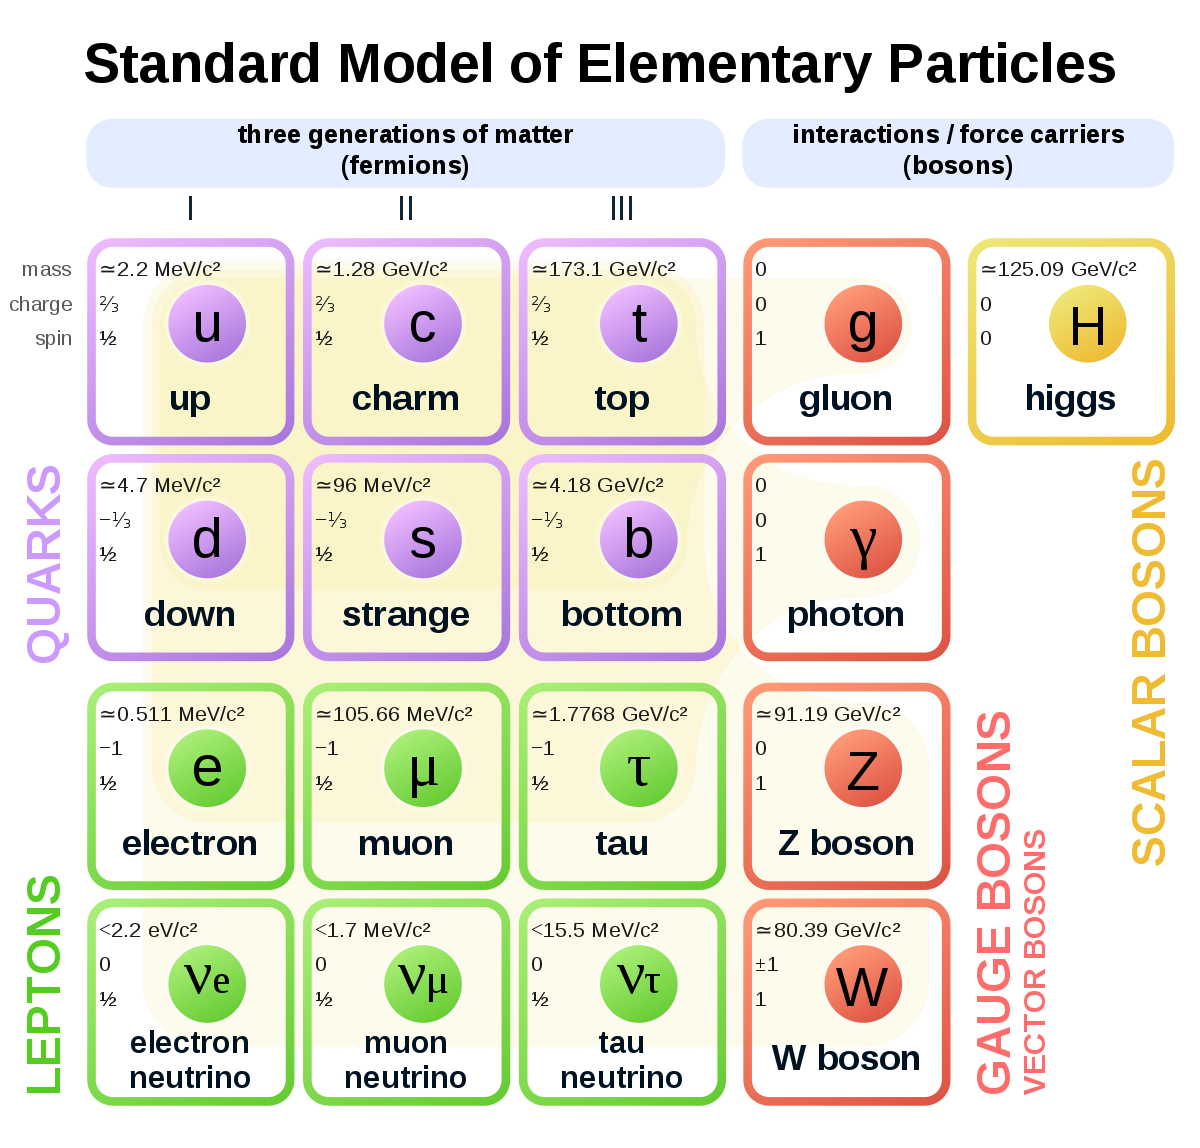
\includegraphics[scale= 0.25]{../Cap1/SM}
\caption{Main constituents of the Standard Model.}
\label{SM}
\end{figure}
The particles involved are characterized by the spin, the mass, and the quantum numbers determining their interactions.
The quarks are subject to all the three forces and, in particular, are the only fermions to
possess a ``colour'' charge, which is responsible of the strong nuclear force, as described by Quantum Chromo Dynamics (QCD). Because of the QCD colour confinement properties, quarks do not exist as free states
but can be experimentally observed only as bound states. The proton and neutron, are composed by three quarks (called baryons). The particle composed by a quark-antiquark are called ``meson''. Quark flavour is conserved in electromagnetic and strong interactions but not in weak ones, as quark mass eigenstates do not correspond to the weak interaction eigenstates.
Their mixing is described by the Cabibbo–Kobayashi–Maskawa (CKM) matrix.
The leptons have no colour charge and are subject only to the electromagnetic and weak
forces. The charged leptons of the three families are respectively denoted as the electron
(e), muon ($\mu$) and tau lepton ($\tau$). The only stable lepton is the electron. To each lepton corresponds a neutrino. The mass of neutrino is unknown but their flavour oscillations prove a non-zero mass~\cite{Balantekin:2013tqa}. 
The gluons, the W$^{\pm}$ bosons, the Z boson and the photon ($\gamma$) are boson that compose the SM gauge sector.
The gluons are the mediators of the strong interactions. They are massless, electrically neutral and carry color quantum number and they can interact with themselves.
The  W$^{\pm}$ and Z bosons are the mediator of the weak interactions. Their mass is $\sim$81 GeV and $\sim$90 GeV respectively. These particles are unstable and decay in other particles. Finally the photon is massless, chargeless, non self-interacting and mediates the electromagnetic
interactions.\\
To summarize, the SM Lagrangian may be written as the sum of three parts:
\begin{equation}
 \mathcal{L}_{SM} = \mathcal{L}_{QCD}+\mathcal{L}_{EWK}+\mathcal{L}_{H}  \:,  \end{equation}
where $\mathcal{L}_{QCD}$ is the quantum chromodynamics Lagrangian that describes the interactions of quarks and gluons, the $\mathcal{L}_{EWK}$ is the the electroweak Lagrangian that describes the interactions of the fermions with the $Z$ and  W$^{\pm}$ bosons. The $\mathcal{L}_{H}$ is the Higgs part of the Lagrangian.
%the Lagrangian symmetries seems to forbid the introduction of mass terms without spoiling its gauge invariance. Higgs’ proposal solves this problem by spontaneously breaking the Lagrangian symmetry (Sec.~\ref{H}).

\subsection*{Quantum Chromodynamics}
The Quantum Chromodynamics (QCD) describes  the interactions of quarks and gluons, mediated by
the strong force through the colour charge.  
The QCD Lagrangian has the local gauge invariance under the  $SU(3)_C$ group and it is given by~\cite{Beringer:1900zz},
\newline
\begin{equation}
\begin{split}
 \mathcal{L}_{QCD}&= \sum_q [\bar{\psi}_{q,a} ( i \gamma^{\mu} \partial_{\mu} \delta_{ab} -g_s \gamma^{\mu} t_{ab}^C A_{\mu}^C -m_q \delta_{ab})\psi_{q,b} \\
&-\frac{1}{4} F_{\mu \nu}^{A}  F^{A \; \mu \nu}] \: , \end{split}  \end{equation}
\newline
where repeated indices are summed over. The $\gamma^{\mu}$ are the Dirac $\gamma$-matrices.
The $\psi_{q,a}$ are quark-field spinors for a quark of flavor $q$ and mass $m_q$, with a color-index $a$
that runs from $a= 1$ to $N_c=R$ 3, i.e. quarks come in three ``colors''. 
Quarks are said to be in the fundamental representation of the $SU(3)$ color group. 
The $A_{\mu}^C$ correspond to the gluon fields, with $C$ running through the eight kinds of gluon.
The $t_{ab}^C$ correspond to eight $3\times 3$ matrices and are the generators of the $SU(3)_C$ group
The quantity $g_S$ is the QCD coupling constant. Finally,
the field tensor $ F_{\mu \nu}^{A}$ is given by,
\newline
\begin{equation}
 F_{\mu \nu}^{A}=  \partial_{\mu} A_{\nu}^A  - \partial_{\nu} A_{\mu}^A -g_{\Large S} f_{ABC}A_{\mu}^B A_{\nu}^C  \: ,   \end{equation}
\begin{equation}
 [t^A, t^B]=i f_{ABC}t^C  \: ,   \end{equation}
\newline
where the $f_{ABC}$ are the structure constants of the $SU(3)_C$ group.
Neither quarks nor gluons are observed as free particles. Hadrons are color-singlet (i.e. color-neutral) combinations of quarks, anti-quarks, and gluons.
The fundamental parameters of QCD are the coupling $g_S$ (or $\alpha_S= \frac{g_S^2}{4\pi}$) and the quark masses $m_q$.
If the quark masses are fixed, there is only one free parameter in the QCD Lagrangian, that is $\alpha_S$. This constant is not a physical observable but
rather  a quantity defined in the context of perturbation theory, which enters in the prediction for experimental observables.


\subsection*{Electroweak Interaction}
The electroweak interactions are based on the gauge group  $SU(2)_L \otimes U(1)_Y$. 
The $SU(2)_L$ group refers to the weak isospin charge ($I$), and $U(1)_Y$ to the weak hyper-charge ($Y$). 
Left-handed ($L$) fermions are paired in $I = 1/2$ isospin doublets, whereas
right-handed ($R$) fermions are $I = 0$ singlets. The presence of these local gauge symmetries
introduces four vector bosons: three for the $SU(2)$ group, the $W_i$ fields ($i = 1, 2, 3$), and
one for $U (1)$, the B field.
This gives rise to a quantum field theory, invariant under local gauge symmetries, whose
Lagrangian is expressed as:
\newline
\begin{equation}
 \mathcal{L}_{EW}= \sum_f \bar{\psi} i \gamma^{\mu }\mathcal{D}_{\mu} \psi -\frac{1}{4} F_{\mu \nu} F^{\mu \nu}  -\frac{1}{4} \vec{E}_{\mu \nu} \cdot \vec{E}^{\mu \nu} \; ,
\end{equation}
where the sum is extended over all the fermions $f$ and where covariant derivatives which
preserve the local  gauge invariance have the following form:
\begin{equation}
\begin{split}
&\mathcal{D}_{\mu} = \partial_{\mu} +ig \vec{W}_{\mu} \cdot \frac{\vec{\tau}}{2} + i\frac{g'}{2} Y B_{\mu}   \; , \\
& F_{\mu \nu}= \partial_{\mu} B_{\nu} -\partial_{\nu} B_{\mu}  \; ,\\
& E_{\mu \nu}^{\alpha}=  \partial_{\mu} W_{\nu}^{\alpha}  \partial_{\nu} W_{\mu}^{\alpha} -g\epsilon^{\alpha \beta \gamma}  W_{\mu}^{\beta} W_{\nu}^{\gamma} \; ,
\end{split}
\end{equation}
\newline
where $\vec{\tau}$ indicates the three Pauli matrices, $g$ and $g'$ are the coupling constants which correspond respectively
to  $SU(2)_L$ and $U(1)_Y$. 
The physical fields are obtained as linear combinations of these fields:
\newline
\begin{equation}
\begin{split}
&A_{\mu}= \sin \theta_W W_{\mu}^3 + \cos \theta_W B_{\mu} \: ,\\
&Z_{\mu}= \cos \theta_W W_{\mu}^3 - \sin \theta_W B_{\mu}  \: ,\\
&W_{\mu}^{\pm}=\frac{W_{\mu}^1 \mp W_{\mu}^2 }{ \sqrt{2}} \: .
\end{split}
\end{equation}
The above equations represent two neutral particles (the photon, described by the $A_{\mu}$
field, and the $Z$ boson) and two charged particles (the $W^+$ and $W^-$ bosons). We have
further introduced the angle $\theta_W$  which is known as the weak mixing angle or Weinberg
angle. Up to here, the theory is necessarily incomplete: all particles it describes are
massless, contradicting experimental evidence. The Lagrangian symmetries, on the other
hand, seem to forbid the introduction of mass terms without spoiling its gauge invariance.
Higgs’ proposal solves this problem by spontaneously breaking the Lagrangian symmetry, Sec.~\ref{H}.

\subsection*{Experimental evidence}
The experimental study  of the Standard Model  has made a quantum leap in the last 30 years. First of all the theory predicted the existence of W$^{\pm}$ and Z bosons in the mass range from 60 to 93 GeV~\cite{doi:10.1142/9789814644150_0006}. 
In 1976 Rubbia, Cline and McIntyre proposed the transformation of an existing high-energy proton accelerator into a proton–antiproton collider as a quick and relatively cheap way to achieve collisions above threshold for W and Z production.  This proposal  was adopted at CERN Super Proton Synchrotron (SPS) collider  and the first  proton–antiproton  collisions were collected in 1981. In the following years the W and Z bosons have been observed by UA1 and UA2 experiments with a mass of 80 GeV and 91 GeV respectively, Fig.~\ref{rubbia_f}. 
\begin{figure}
\centering%
\subfigure[]%
{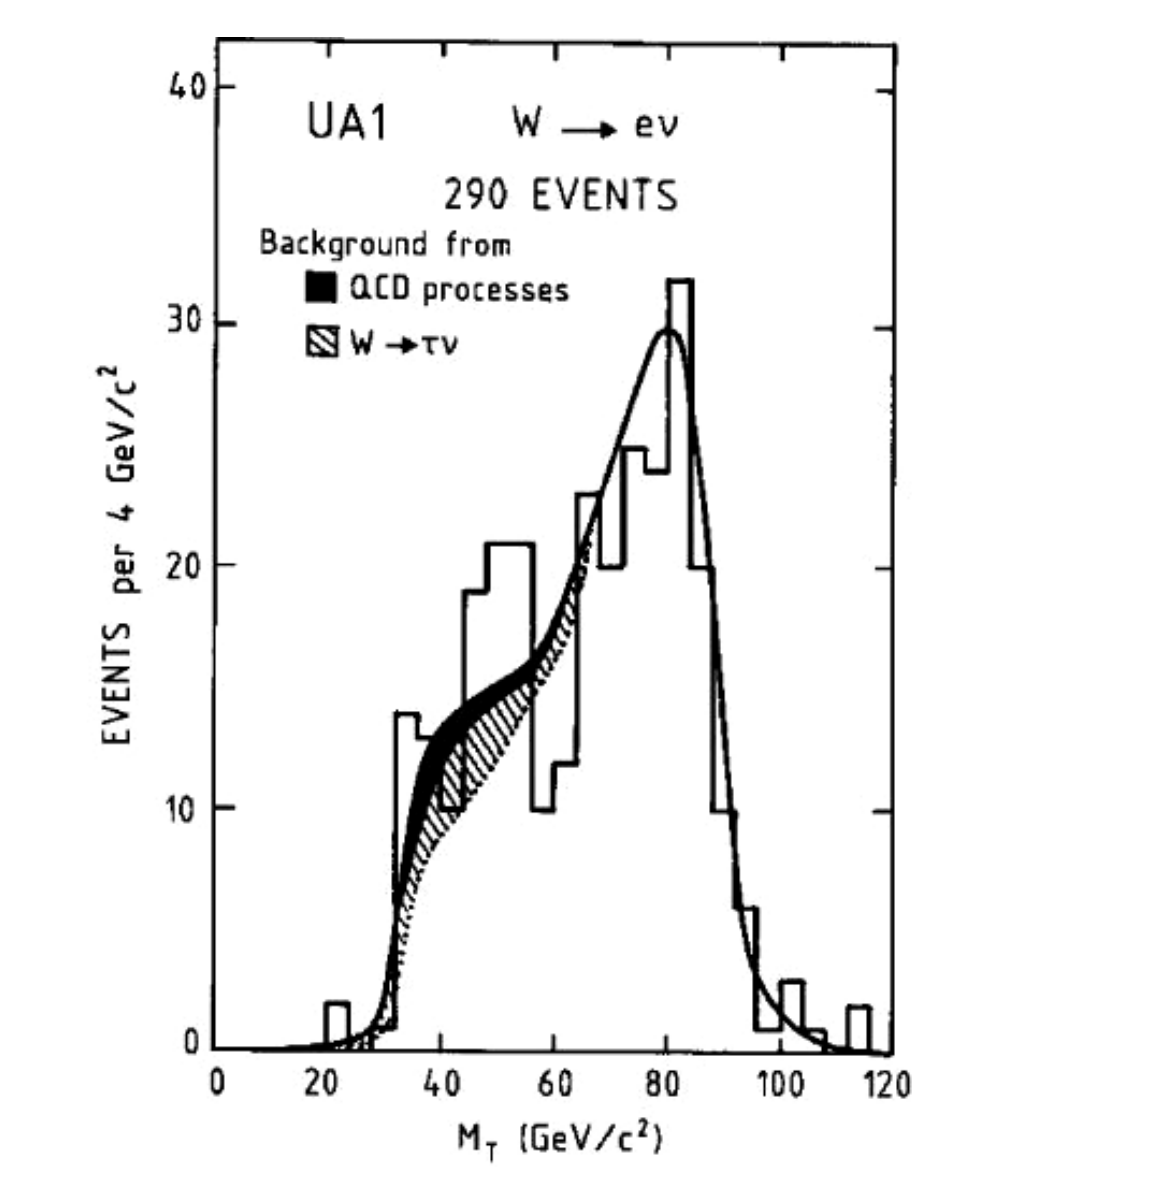
\includegraphics[scale= 0.66]{../Cap1/rubbia_W}}
\subfigure[]%
{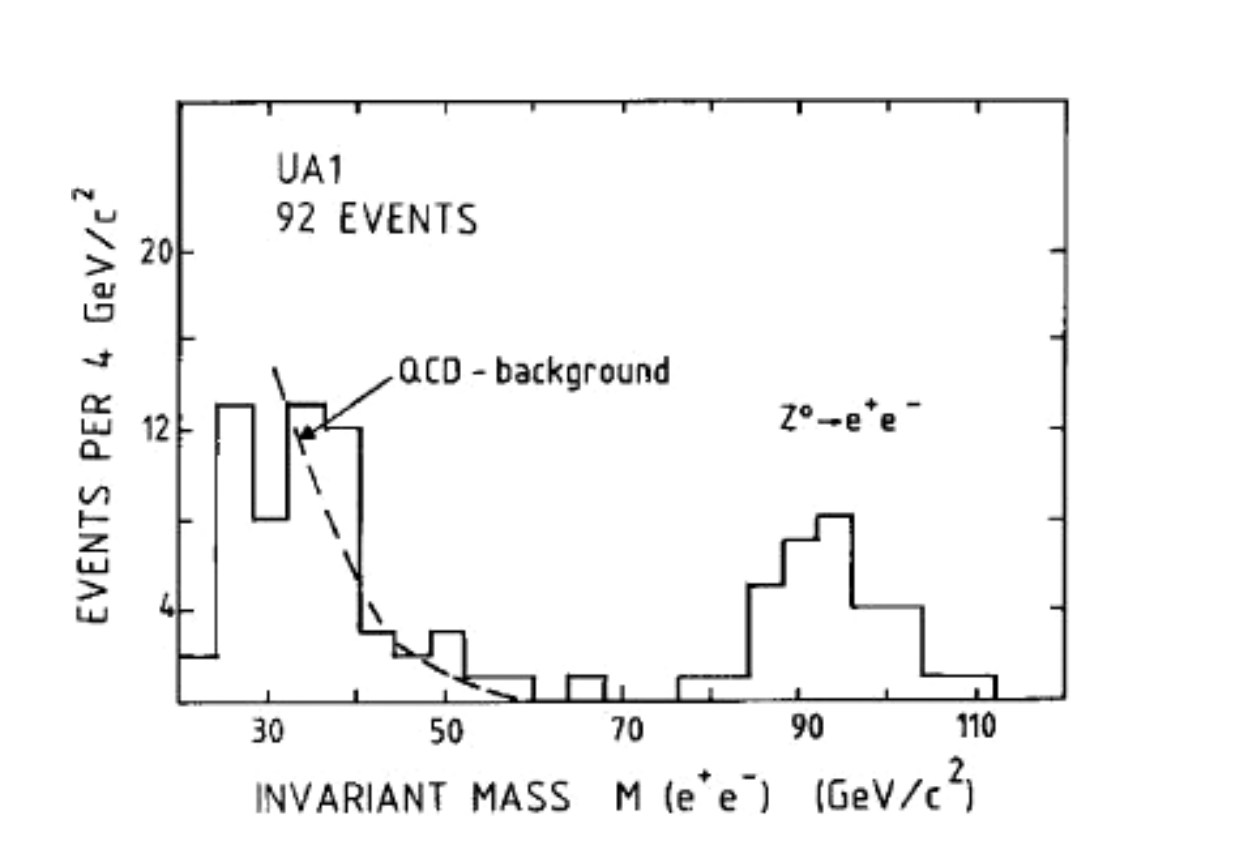
\includegraphics[scale= 0.66]{../Cap1/rubbia_Z}}
\caption{(a) Transverse mass distribution for all W$\to e \nu$ events recorded by UA1 between 1982 and 1985. (b) Invariant mass distribution of all $e^+e^-$
pairs recorded by UA1 between 1982 and 1985}
\label{rubbia_f}
\end{figure}
With the electron-positron colliders at a center-of-mass energy equal to $Z$ mass, precise measurements of the fundamental parameters of electroweak theory could be made.  In 1989, two  $e^+e^-$ colliders operation started:
the Stanford Linear Collider (SLC) at SLAC,  and the circular Large Electron
Positron collider (LEP) at CERN. Precision electroweak tests covering the measurements at the Z pole  have been conducted by SLC and LEP experiments.
W boson properties were also measured at the LEP collider, which reach 209 GeV center-of-mass energy, well above the threshold for $W^+W^-$ pair production,  Fig.~\ref{alt}. The results of measurements confirmed the SM prediction. 
\begin{figure}
\centering
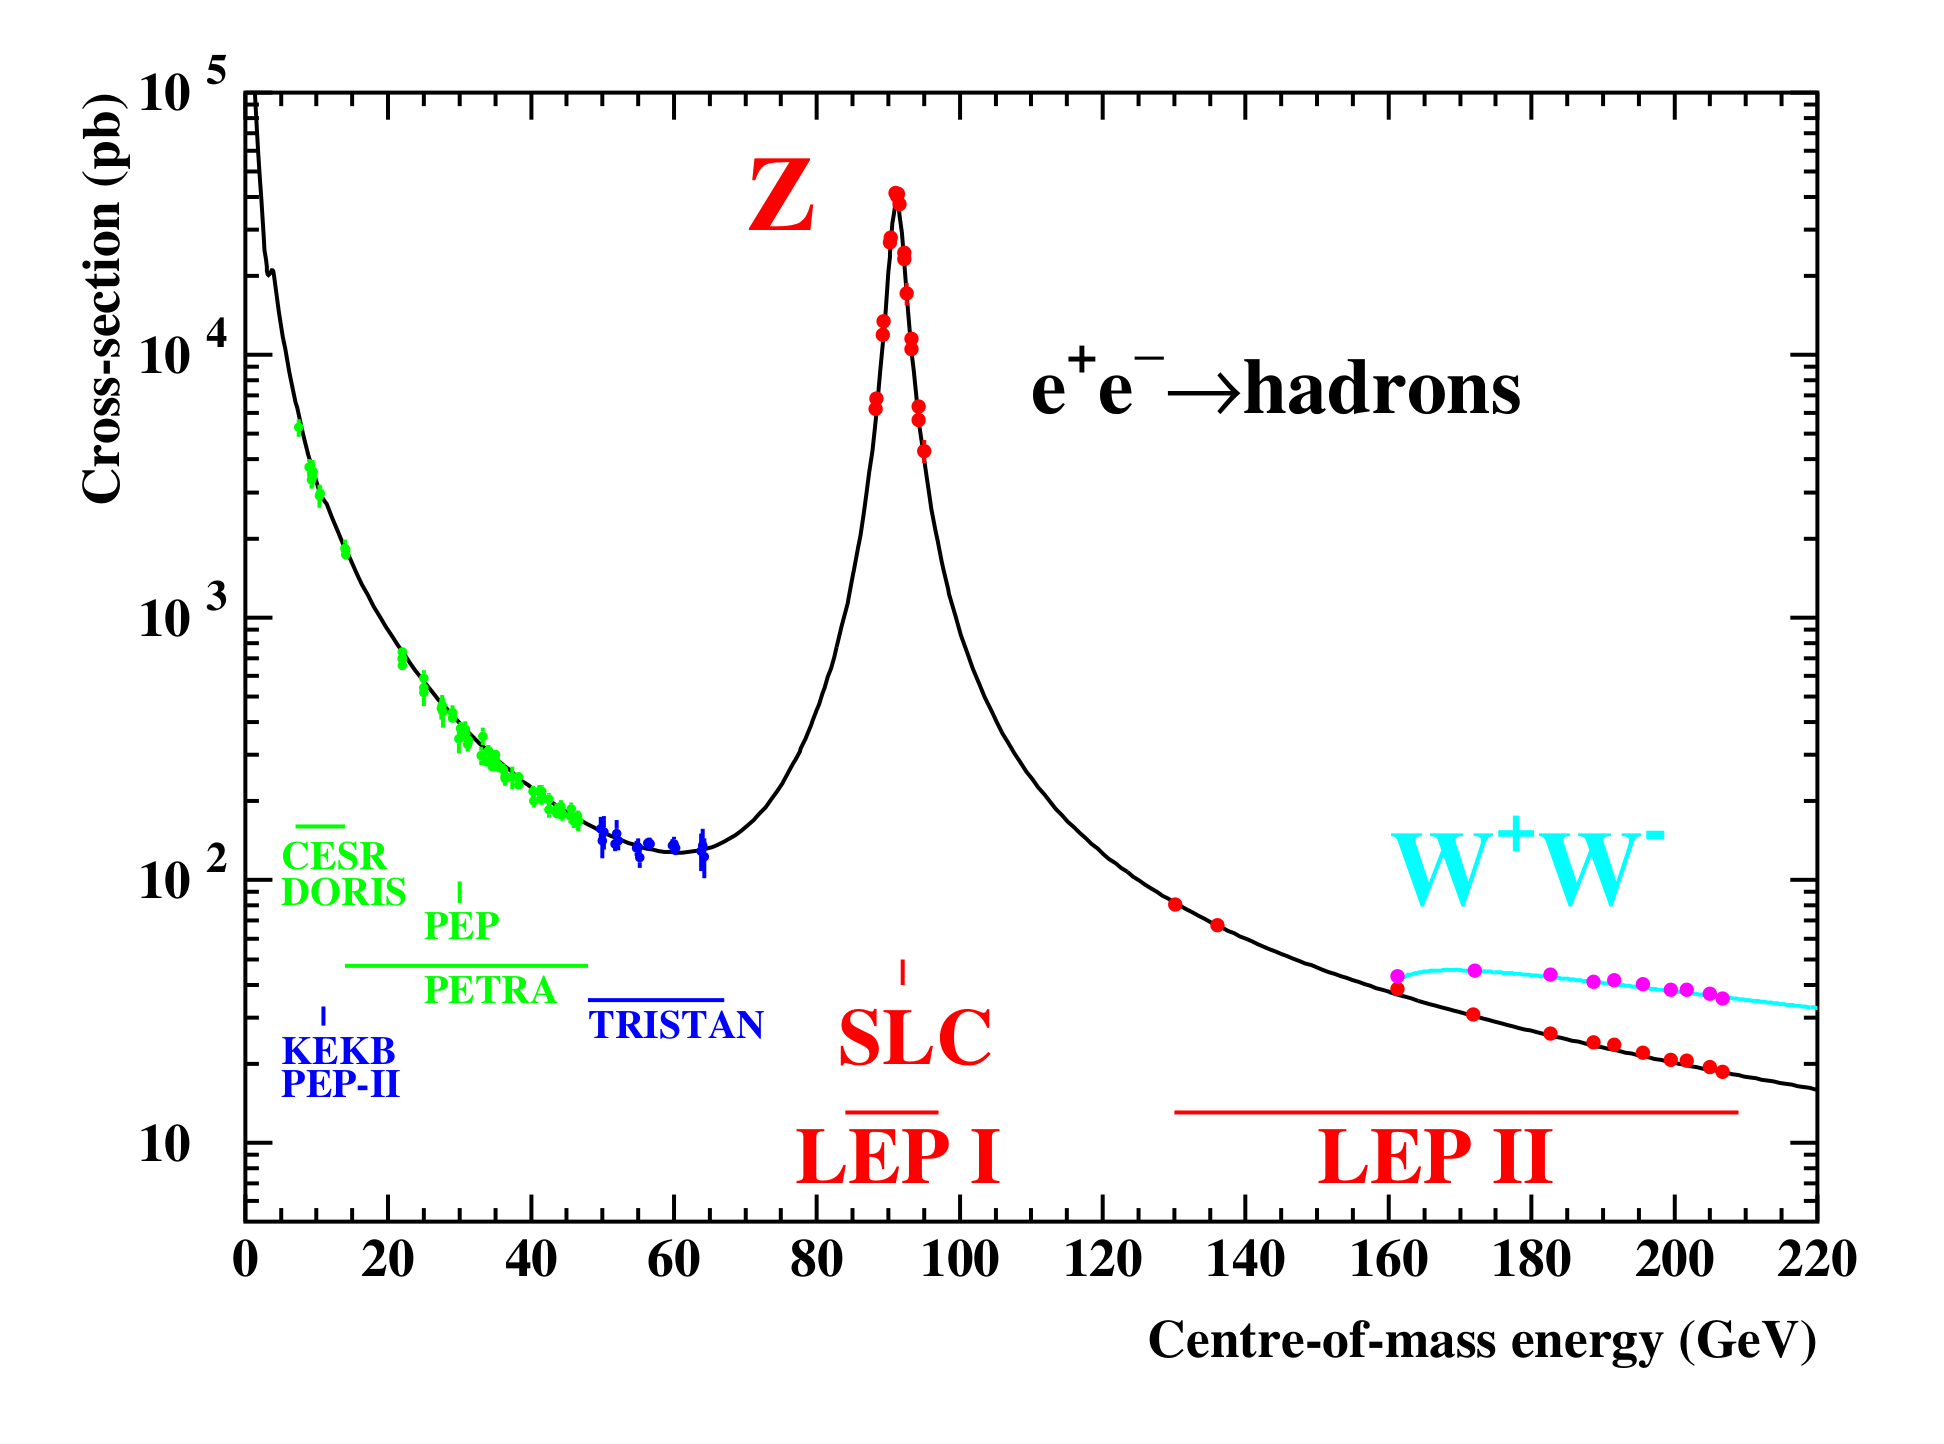
\includegraphics[scale= 0.5]{../Cap1/alt_Z}
\caption{The cross-section for the production of hadrons in $e^+e^-$ annihilations. The measurements are shown as dots with error bars. The solid line shows the prediction of the SM}
\end{figure}
\begin{figure}
\centering
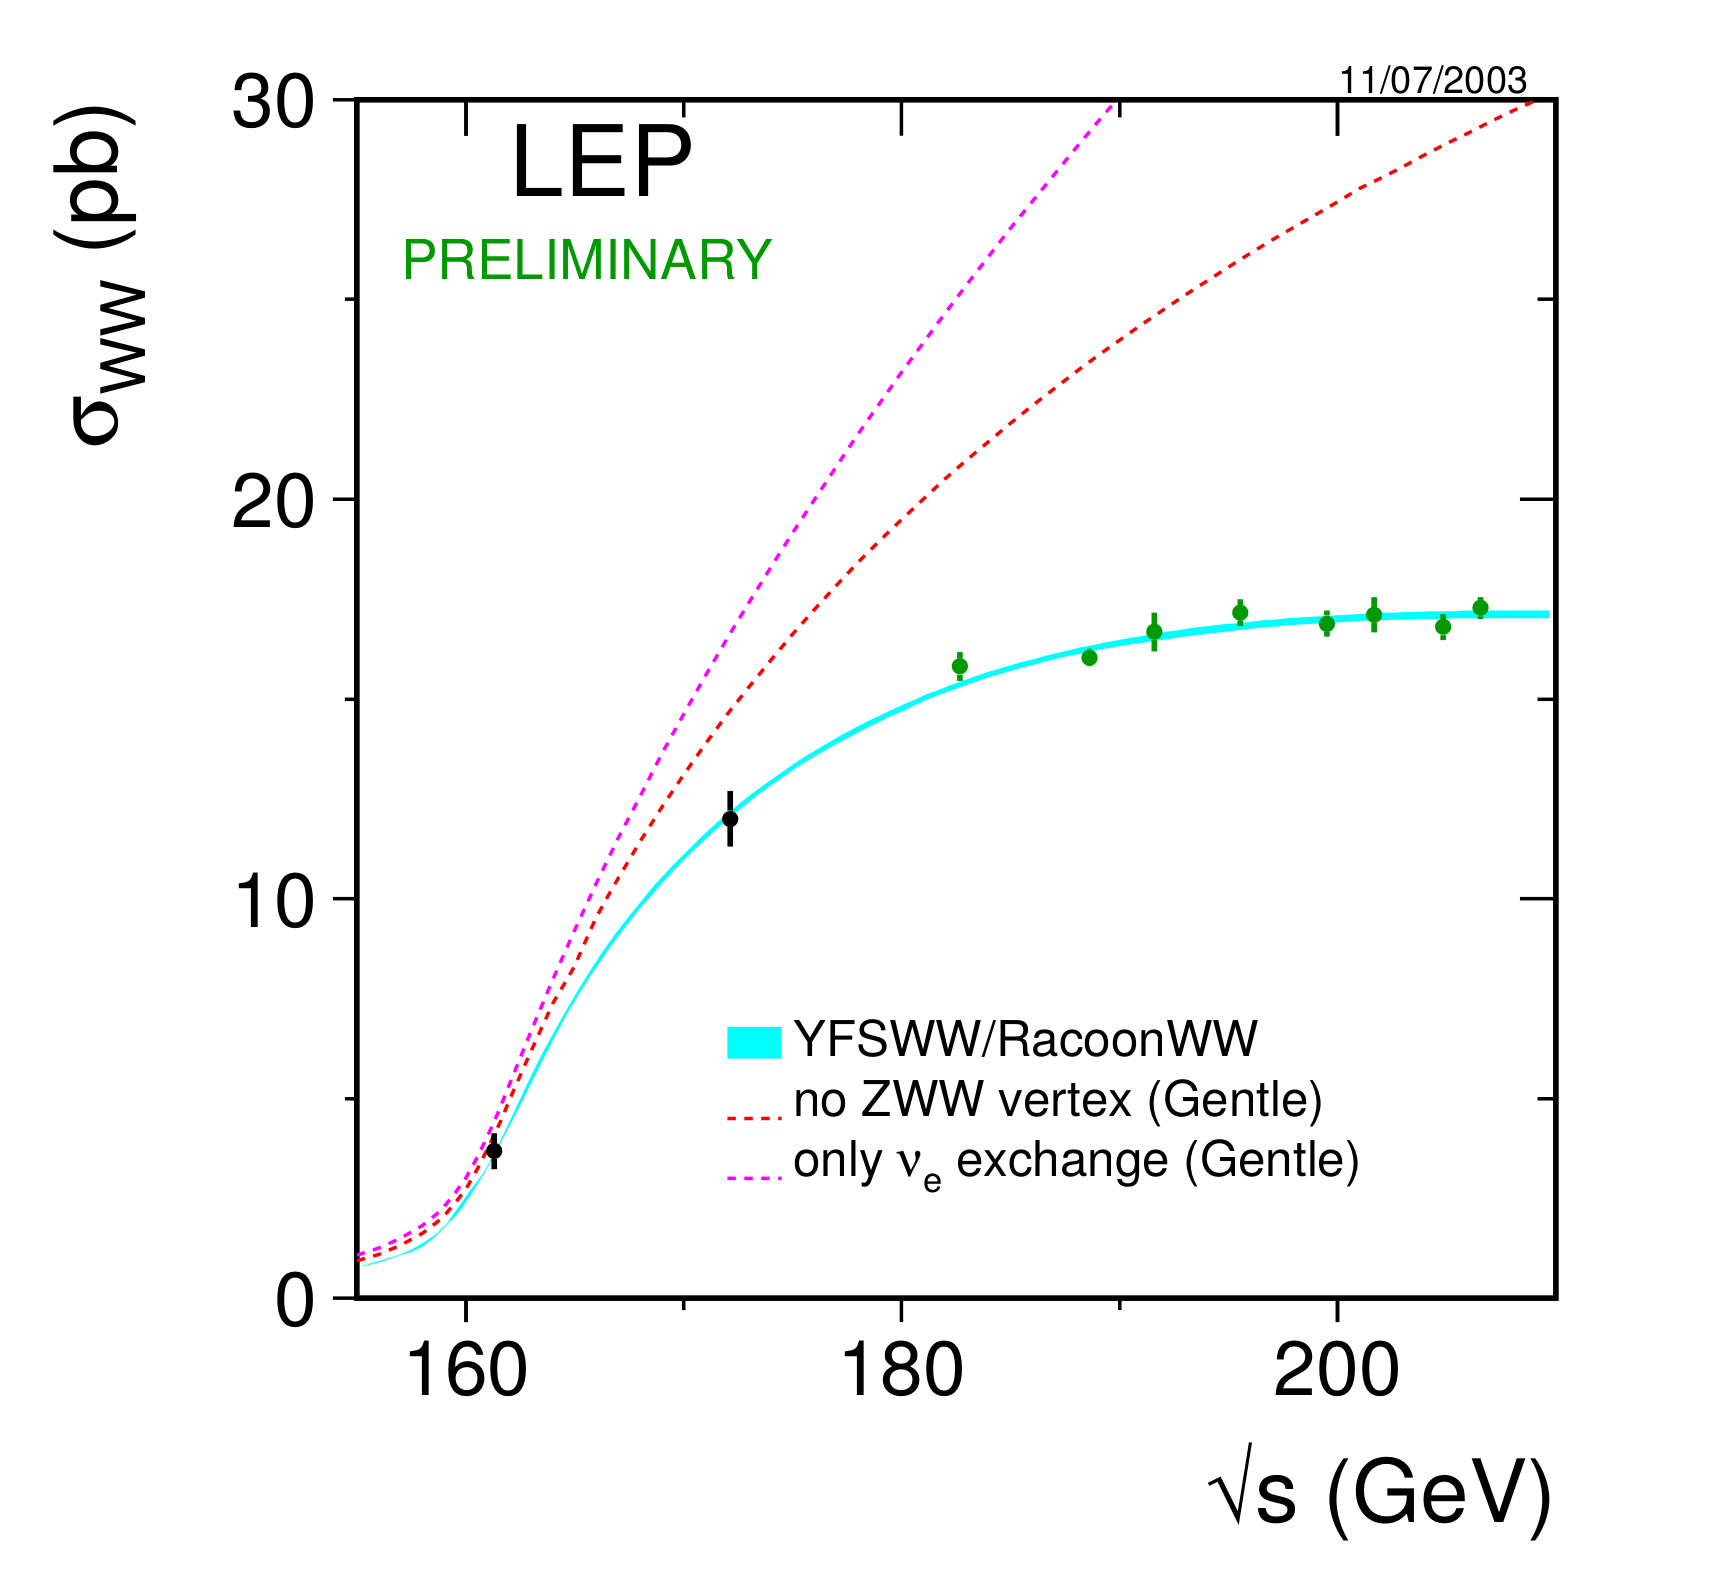
\includegraphics[scale= 0.3]{../Cap1/alt_W}
\caption{ The measured W-pair production cross section compared to the SM and alternative
theories not including trilinear gauge couplings.}
\label{alt}
\end{figure}
The next missing SM piece was top quark. It was a necessary component of the SM of electroweak interactions, but there was no consistent theoretical guidance as to what its mass should be. The only way to observe a top quark with such a high mass was at the collider with the highest-energy, the Tevatron antiproton-proton collider at Fermilab. The existence of the top quark was firmly established in 1995 with simultaneous announcements by both the CDF~\cite{PhysRevLett.73.225} and the DO~\cite{D0:1995jca} experiments with results that demonstrated a mass of around 174 GeV, Fig.\ref{Wells2004_Article_ExperimentalTestsOfTheStandard}.
After the top quark discovery, the only missing part to the SM was the Higgs boson particle  that has been observed at ATLAS and CMS experiment at LHC proton-proton collider at CERN in 2012 (see Sec.\ref{H}).  
\begin{figure}
\centering
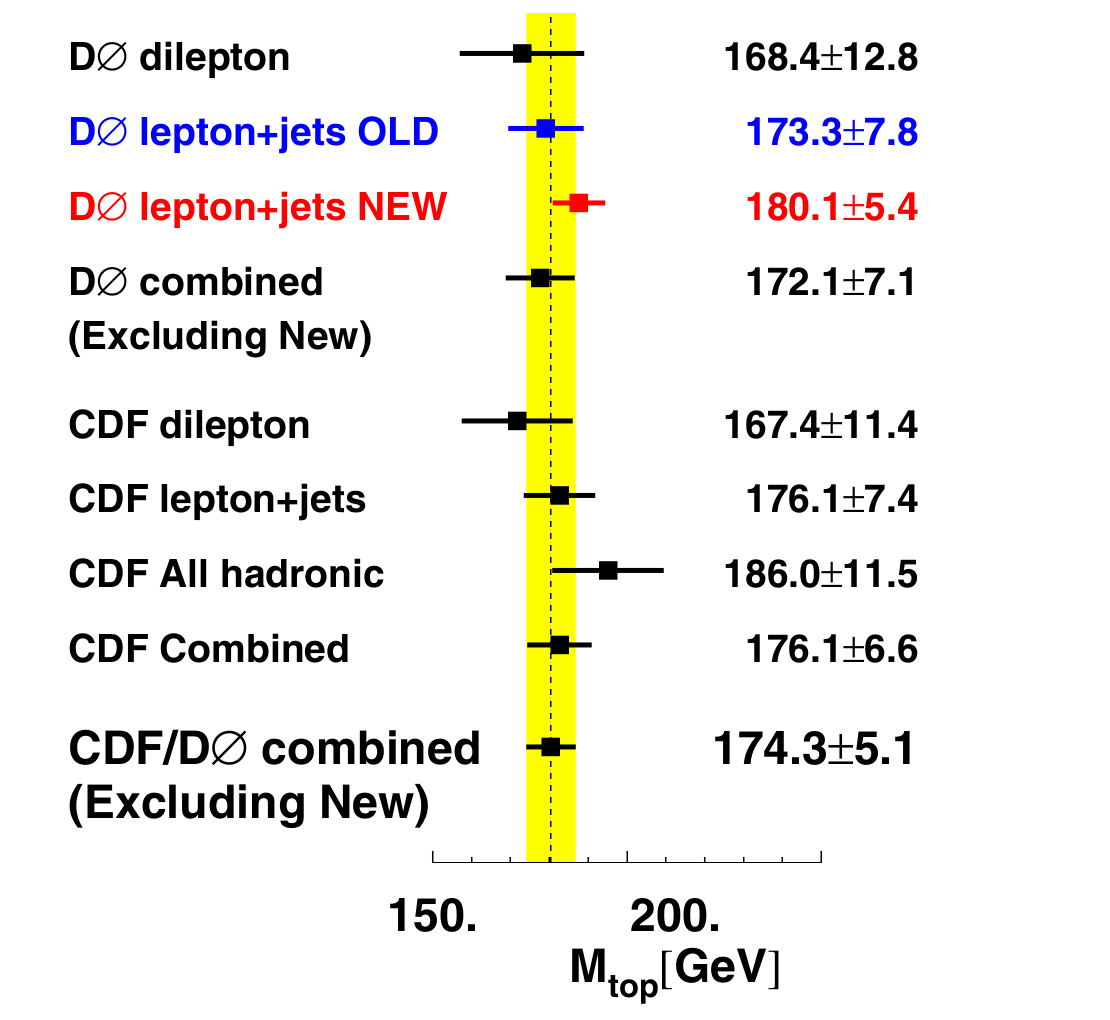
\includegraphics[scale= 1]{../Cap1/Wells2004_Article_ExperimentalTestsOfTheStandard}
\caption{Top quark mass measurements.}
\label{Wells2004_Article_ExperimentalTestsOfTheStandard}
\end{figure}




\section{The Higgs Boson}
\label{H}
A  Lagrangian is said to have a symmetry when it is invariant under a group of transformations. 
However the fact that the weak gauge bosons have a mass different from zero indicates that
the gauge symmetry is broken. Also the fermion masses can
not be included without violating gauge symmetry in the $\mathcal{L}_{QCD}$.
The mass terms can be introduced with the Spontaneous Symmetry Breaking Mechanism, adding  $\mathcal{L}_{H}$, that gives mass to the weak bosons and fermions and leaves the photon massless. This mechanism has been proposed in 1964 independently by Higgs~\cite{HIGGS1964132} and Brout and Englert~\cite{PhysRevLett.13.321}. With the spontaneous symmetry breaking mechanism, a  new particle which couples  to the massive fermions and to the boson emerges. This particle is called Higgs boson and its mass is a free parameter of the theory. In 2012, 48 years after this hypothesis was formulated, the Higgs boson has been observed by ATLAS~\cite{Aad:2012tfa} and CMS~\cite{Chatrchyan:2012xdj} experiments at LHC.


\subsection*{The Brout–Englert–Higgs mechanism}
The symmetry of SM Lagrangian, $\mathcal{L}_{SM}$, is $SU(2)_L \otimes U(1)_Y \otimes SU(3)_C$, where $L$, $Y$ and $C$ refers to isospin, hypercharge and color quantum numbers, respectively. To break the symmetry,  a  scalar field $\Phi$ (Higgs field) is introduced. 
The field is an  isospin doublet ($SU(2)_L$):
\newline
$$
\Phi=
\left(
\begin{array}{c}
\Phi^+   \\
\Phi^0 \\
\end{array}
\right)
=\frac{1}{\sqrt{2}}
\left(
\begin{array}{c}
\Phi_1 + i\Phi_2   \\
\Phi_3 + i\Phi_4  \\
\end{array}
\right)
$$
\newline
where $\Phi_j$ with $j=1,2,3,4$ are real fields used to manifest the complexity of $\Phi^+$ and  $\Phi^0$. The simplest Lagrangian of a self-interacting scalar field is,
\begin{equation}
 \mathcal{L}_{H}= (D^{\mu} \Phi^{\dag})(D_{\mu} \Phi) -\mu^2 \Phi^{\dag}\Phi - \lambda(\Phi^{\dag}\Phi)^2 \; , \end{equation}
where $\lambda$ needs to be positive for the potential to be bounded from below and $\mu^2$
 is a mass term for the $\Phi$ field.
The ground state (vacuum) of the theory is defined as the state where the energy density is at a minimum.
If the $\mu$ parameter is chosen so that $\mu^2<0$, the symmetry of the potential may be broken,
and  the minimum value is,
\newline
\begin{equation}
v\equiv
\sqrt{\frac{-\mu^2}{\lambda}}=\Phi^{\dag}\Phi \; .
\label{min}
\end{equation}
The choice for the sign of the
parameters $\mu^2$ and $\lambda$ gives to the potential $V(\Phi)= \mu^2 \Phi^{\dag}\Phi + \lambda(\Phi^{\dag}\Phi)^2$ the ``mexican hat'' shape, as illustrated in Fig.~\ref{higgspotential}.
\begin{figure}
\centering
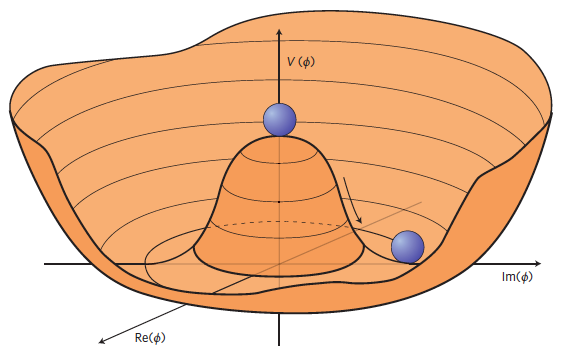
\includegraphics[scale= 0.4]{../Cap1/higgspotential}
\caption{Higgs fields potential with two degree of freedom.}
\label{higgspotential}
\end{figure}
In the perturbation theory, the $\Phi$ fields is expanded around the minimum, that is chosen among the set of states which satisfy Eq.~\ref{min}. All this states break the rotational symmetry of the Lagrangian.
The $\Phi$ field is expressed as, 
\begin{equation}
\Phi= \frac{1}{\sqrt{2}} 
\left(
\begin{array}{c}
0   \\
v +h(x) \\
\end{array}
\right) .
\end{equation}
The $h(x)$ field gives a particle with mass equal to,
\begin{equation}
m_H=\sqrt{2}\mu=v\sqrt{2 \lambda} \; ,
\label{mass_H}
\end{equation}
that is a free parameter of the theory. However some theoretical constrains could be imposed. The value of $v$ parameter in Eq.~\ref{mass_H} could be determinate by the Fermi constant, $G_F$, as,
\begin{equation}
v=\frac{2m_W}{g}=(\sqrt{2} G_F)^{-1/2} \; ,
\end{equation}
with the actual $G_F$ measurements obtained with the muon lifetime~\cite{vanRitbergen:1999fi}, a value  of~$\sim$~250 GeV is obtained for  $v$. However the  model is not predictive on the value of the $\lambda$ parameter. Nevertheless, additional theoretical arguments place approximate upper and
lower bounds on $m_H$~\cite{Beringer:1900zz}. The lower bound on the Higgs mass is given by  the vacuum state stability, that leads to requiring $\lambda$ to be
positive at all energies. The upper edge is imposed by the Planck scale. So a Higgs boson in a range of 130 $<m_H<$ 180 GeV is consistent with the theory.
 
\subsection*{The Higgs boson at LHC}
The Higgs boson  has been searched in several experiments (Fig.~\ref{650px-CMS_Higgs-event}) located  at different  colliders (LEP, SLC, Tevatron) without a clear evidence of such particle.
Therefore,  the Large Hadron Collider, a  proton-proton collider located at CERN,  has been designed with the primary goal of discovering or excluding the Higgs 
boson. 
In a proton-proton collision the Higgs boson can be produced in different ways: via gluon-gluon fusion, the vector boson fusion (VBF), the vector-boson associated production and the top-quark associated production. Below are the details of the different mechanisms:
\begin{itemize}
\item \textit{Gluon-gluon fusion} ($gg \rightarrow H$): this is the main Higgs boson production mode. Here a couple of gluons interact via a heavy quark loop and give rise to a Higgs boson.
\begin{figure}[h]
\centering
\vspace{0.5cm}
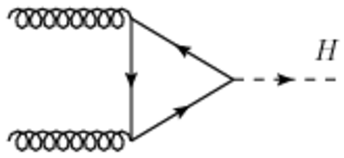
\includegraphics[scale= 0.7]{../Cap1/gg}
\end{figure}
\item \textit{Vector Boson Fusion} (VBF) ($qq \rightarrow qqH$): each incoming quarks emits a virtual W or Z boson that interact generating a Higgs boson.
The quarks after emitting the vector bosons proceed in the forward direction and represent the peculiar signature of this production mode.
\begin{figure}[h]
\centering
\vspace{1cm}
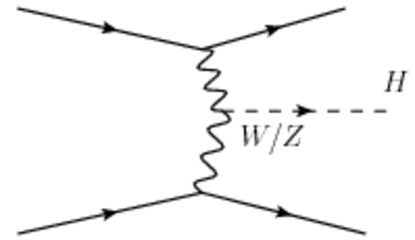
\includegraphics[scale= 0.6]{../Cap1/vbf}
\end{figure}
\item \textit{Vector boson associated production} (or \textit{Higgsstrahlung}):  the Higgs boson is emitted from a W$^{\pm}$ or a Z boson which has
been produced by a pair  quark-antiquark.
\begin{figure}[h]
\centering
\vspace{0.5cm}
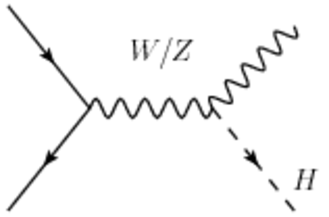
\includegraphics[scale= 0.6]{../Cap1/hlung}
\end{figure}
\item \textit{Top-quark associated production}: a pair of top quarks, originated from
the splitting of two incoming gluons, interacts to yields to a Higgs boson. 
 \begin{figure}[!htbp]
\centering
\vspace{0.5cm}
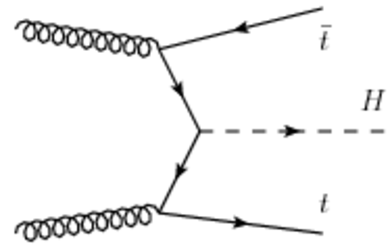
\includegraphics[scale= 0.6]{../Cap1/tt}
\end{figure}  
\end{itemize}
The Higgs boson cross section of the different production modes, depend on the center of mass energy of the collider and by the supposed mass of the particle.
The cross section increases with the energy of the colliding particles $(\sqrt{s})$ and decreases with the mass of the boson, $m_H$. The second behaviour is shown in
Fig.~\ref{prod}. The Higgs boson is an unstable particle and decays in a variety of different finale states, Fig~\ref{br}. For a Higgs boson of mass $m_H \sim$ 125 GeV (that is the mass measured by ATLAS and CMS) the channel with the largest branching ratio is in $\bar{b}b$ quark, followed by the $W^+W^-$, $\tau^+ \tau^-$ and $ZZ$ channels.
\begin{figure}
\centering
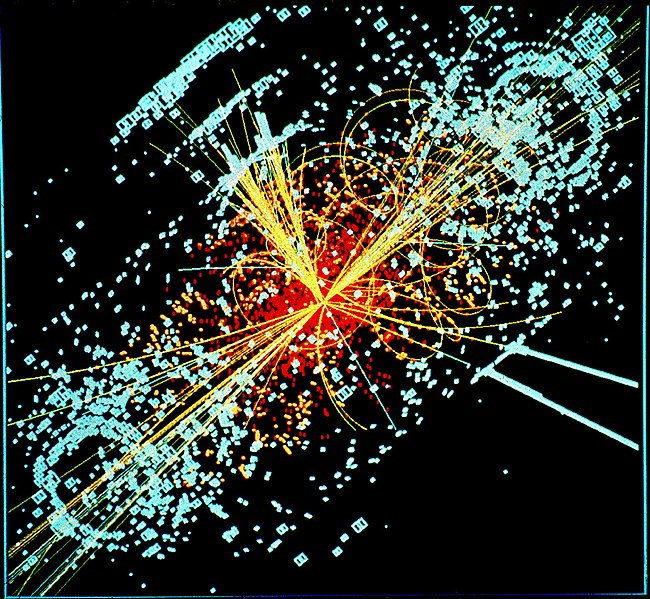
\includegraphics[scale= 0.4]{../Cap1/650px-CMS_Higgs-event}
\caption{An example of simulated data modeled for the CMS particle detector on the Large Hadron Collider (LHC) at CERN.}
\label{650px-CMS_Higgs-event}
\end{figure}  

\subsection*{Experimental Results}
The discovery or exclusion of the SM Higgs boson was one of the primary scientific goals of LHC. On the 4th of July 2012, as the observation of a new boson by the ATLAS~\cite{Aad:2012tfa} and the CMS~\cite{Chatrchyan:2012xdj} collaborations has been announced, as an excess of events near 125 GeV was reported by both experiments, Fig.~\ref{disc_hig}. 
%In 2012 the proton-proton centre of mass energy was increased to 8 TeV and by the end of June an additional integrated luminosity
%of more than 5 fb$^{-1}$ had been recorded by each of these experiments, thereby enhancing significantly the sensitivity of the search for the Higgs boson.
Latest results from both the experiments confirm that  the properties of the discovered particle are consistent with the hypothesis of
being the Higgs boson predicted by the Standard Model.
\begin{figure}
\centering%
\subfigure[]%
{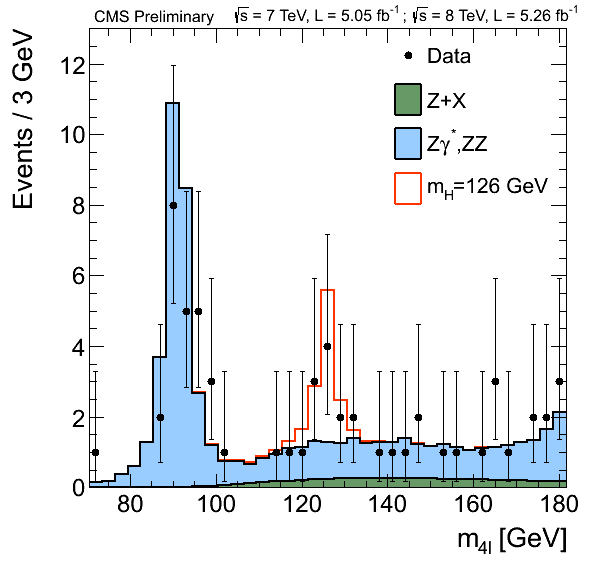
\includegraphics[scale= 0.55]{../Cap1/004}}
\subfigure[]%
{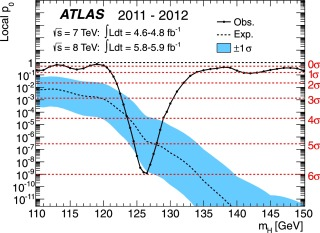
\includegraphics[scale= 0.3]{../Cap1/009}}
\caption{(a) Distribution of the four-lepton invariant mass for the ZZ$\to 4 \ell$ analysis of CMS.  (b) The observed (solid) $p_0$ local as a function of $m_H$ in the low mass range in ATLAS detector. }
\label{disc_hig}
\end{figure}
The measurements of Higgs boson couplings via exclusive production modes and decay channels, of its spin-parity, and
of its differential production cross section, need to be thoroughly investigated to verify
that they correspond precisely to the SM predictions. It is being done using the new data, collected from 2015 at LHC with  increased center-mass-energy of 13 TeV.
Precision measurements of the Higgs boson’s properties can help understanding   why the Higgs
boson mass is near the electroweak scale. In particular, it is important to measure the  Higgs boson  couplings. In the $k$-framework~\cite{Heinemeyer:2013tqa}  coupling modifiers are introduced in order to test for deviations in the couplings of the Higgs boson to other particles.  
Indeed, the couplings to up and down type fermions can be nonuniversal.  Additionally, in these models,
it is possible that the Higgs boson will couple differently to fermions ($k_F$) and vector bosons ($k_V$), Fig.~\ref{Figure_016}. This results so far shows a good agreement among the experimental  data and the theory.
\begin{figure}
\centering
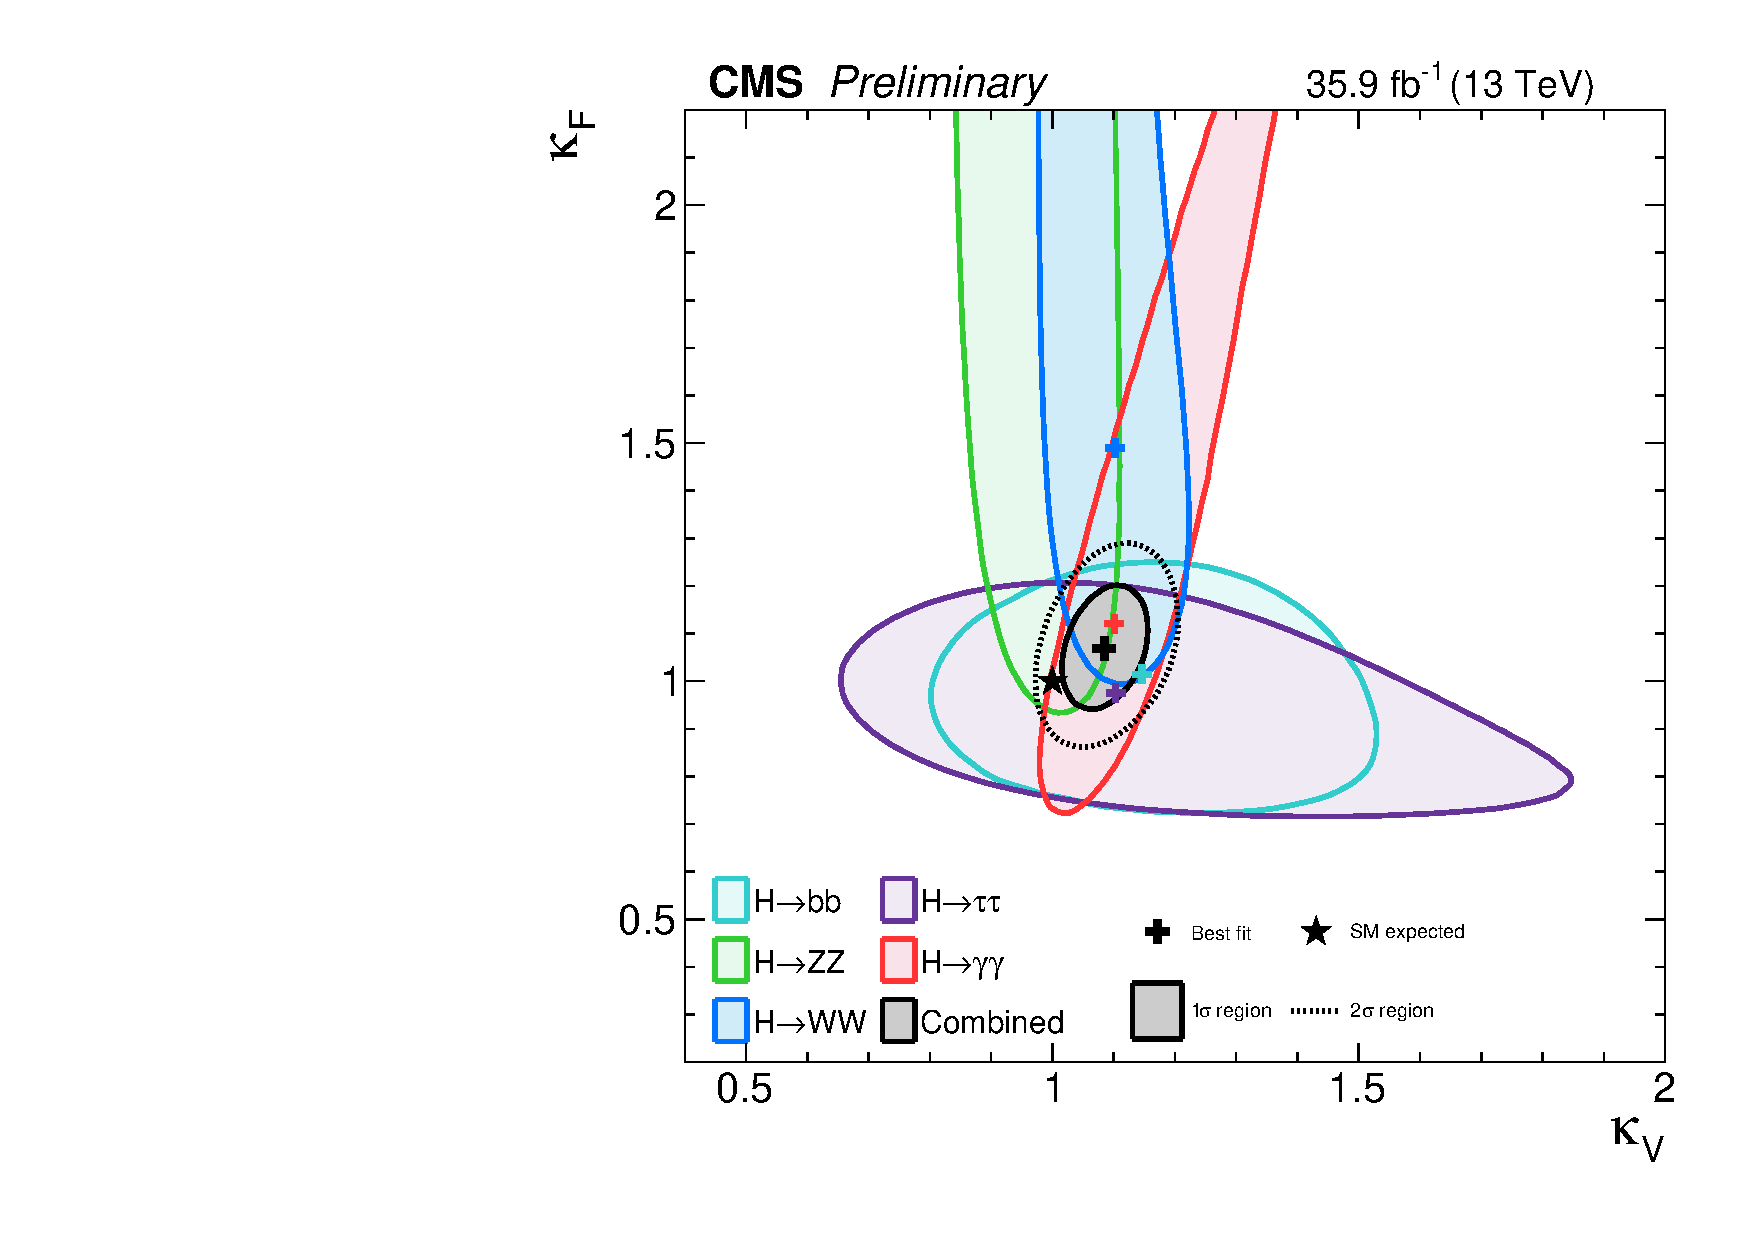
\includegraphics[scale= 0.5]{../Cap1/Figure_016}
\caption{The  CL regions in the $k_F$ vs $k_V$ parameter space for the model assuming a common scaling of all the vector boson and fermion couplings.}
\label{Figure_016}
\end{figure}  



%\subsection*{Higgs boson to WW channel}

\section{New Scalar Particles}
\label{NSP}


\subsection*{Open Questions} The Standard Model is presently the best description of the subatomic nature, but this theory does not provide a complete picture of the world. Sure enough there are still open questions: the gravity is not described in the model, the explanation of the dark matter is not clear and the  neutrino mixing and mass are not well understood.
The gravity is one of the four fundamental interactions but it is not described in the  SM. It is so different from the three other
forces. The purpose to establish a common theory that describe all forces is so difficult. The gravity is described in the  Einstein’s General Relativity (GR) theory. To combine the  SM with the GR it is necessary a quantum theory with a new field associated to gravity  as mediator: a spin 2 particle called graviton. Right now there are no experimental evidence of the existence of this kind of particle. 
An other deficit of the SM regards the dark matter. In fact, from astronomical observations, only the 5\% of the  matter and energy content of our universe is formed by the ordinary matter (hadrons and leptons), the other 95\% is composed by dark matter ($\sim$ 25\%) and dark energy ($\sim$ 70\%). The SM does not offer good candidates or explanations for the dark matter and dark energy problems.
Concerning the neutrinos, in the SM they were assumed massless. However flavour oscillation implies that they must have non zero mass differences.
It is not clear if the small neutrino masses  can arise from the same electroweak symmetry breaking mechanism that
is in act for the other SM particles.\\
\newline
These open questions represent  deficiencies of the Standard Model. 
The presence of a hidden sector, defined here to mean extra states that
have no SM gauge charge but are charged under some other exotic gauge symmetry, does not necessarily solve any of the problems above. However, in order to identify whether the SM Higgs sector is complete,  the searches of additional heavy scalars are performed.  They would prove the presence of beyond-the-SM (BSM) physics in the form of a non-minimal Higgs sector~\cite{Robens:2015gla}. The existence of sibling Higgs boson, denoted $X$, is motivated in many BSM scenarios, so the research in the full mass range accessible at colliders  remains one of the main objectives of the experimental community. This  program  needs  to  be continued within the full mass range that is accessible to current and future experiments.
\newline
\subsection*{Higgs Singlet Extension}
The simplest extension of the SM Higgs sector consist in adding to the complex $SU(2)_L$ doublet $\Phi$ a real scalar  $S$ which is a singlet under all SM gauge groups.  The most general gauge-invariant and renormalisable scalar Lagrangian is,
\newline
\begin{equation}
 \mathcal{L}_s = (D_{\mu} \Phi )^{\dagger}  \: D_{\mu} \Phi  +  \partial^{\mu}S   \partial_{\mu}S -V(\Phi, S)   \: ,  \end{equation}
\newline
where $V(\Phi, S) $ is the scalar potential,  
\newline
\begin{equation}
 V(\Phi, S)= -m^2   \Phi ^{\dagger}\Phi -\mu^2 S^2 +\lambda_1 (\Phi ^{\dagger}\Phi)^2 +\lambda_2 S^4 + \lambda_3 \Phi ^{\dagger}\Phi S^2 \: . \end{equation}
\newline
Here, $Z_2$ ($S \rightarrow -S$) symmetry is imposed which forbids additional terms in the potential.
To determine the condition for $V(\Phi, S)$ to be bounded from below, it is necessary to study its behaviour for large field values.
The two vacuum expectation values (VEVs) are defined as,
\begin{equation}
\langle \Phi \rangle \equiv \left(
\begin{array}{c}
0  \\
\frac{v }{\sqrt{2}}  \\
\end{array}
\right)
, \qquad 
\langle S \rangle \equiv \frac{x }{\sqrt{2}}  \:,  \end{equation}
with v and x real and non-negative.
With this definition of the VEVs, the extrema of V are determined using the following set of equations: 
\newline
\begin{equation}
\frac{\partial V}{\partial v}(v,x)= v \cdot (-m^2+ \lambda_1 v^2+ \frac{\lambda_3}{2}x^2 )=0 , \end{equation}
\begin{equation}
\frac{\partial V}{\partial v}(v,x)= x \cdot (-\mu^2+ \lambda_2 x^2+ \frac{\lambda_3}{2}v^2 )=0 \: . \end{equation}
\newline
The physically interesting solutions have $v,x>0$:
\newline
\begin{equation}
v^2=\frac{\lambda_2 m^2-\frac{\lambda_3}{2} \mu^2}{\lambda_1 \lambda_2- \frac{\lambda_3^2}{4}} \; , \end{equation}
\begin{equation}
x^2=\frac{\lambda_1 \mu^2-\frac{\lambda_3}{2} m^2}{\lambda_1 \lambda_2- \frac{\lambda_3^2}{4}} \; . \end{equation}
\newline
For the determination of the extrema we evaluate the Hessian matrix:
\begin{equation}
\mathcal{H}(v,x) \equiv \left(
\begin{array}{cc}
\frac{ \partial ^2 V}{\partial v^2} &  \frac{\partial ^2 V}{\partial v \partial x}  \\
\\
\frac{\partial ^2 V}{\partial v \partial x}   & \frac{\partial ^2 V}{\partial x^2} \\
\end{array}
\right) =     \left(
\begin{array}{lr}
  2 \lambda_1 v^2 &  \lambda_3 vx \\
\lambda_3 vx & 2 \lambda_2 x^2 \\ 
\end{array} \right) \; .\end{equation}
\newline
So, the scalar potential $V(\Phi, S)$ is bounded from below if the following conditions are fulfilled,
\begin{equation}
 4 \lambda_1  \lambda_2 - \lambda_3^2 >0   \: , \end{equation}
\begin{equation}
 \lambda_1 , \lambda_2  >0    \: , \end{equation}
where if the first condition is fulfilled, the extremum is a local minimum. The
second condition , guarantees that the potential is bounded from below for large field values.
The Higgs fields, $\Phi$ and $S$, have non-zero vacuum expectation, denoted by $v$ and $x$, respectively.
Following the unitary-gauge prescription, the Higgs fields is given by,
\newline
\begin{equation}
{\mathcal H} \equiv \left(
\begin{array}{c}
0  \\
\frac{\tilde{h}+v }{\sqrt{2}}  \\
\end{array}
\right)
, \qquad 
S \equiv \frac{h'+x }{\sqrt{2}}  \: . \end{equation}
\newline
Expansion around the minimum leads to the squared mass matrix
\newline
\begin{equation}
{\mathcal M}^2 = \left(
\begin{array}{cc}
2 \lambda_1^2 v^2 & \lambda_3 vx  \\
\lambda_3 vx & 2 \lambda_1^2 x^2 \\
\end{array}
\right)
\: , \end{equation}
\newline
with the mass eigenvalues
\begin{equation}
 m_h^2=  \lambda_1 v^2 + \lambda_2 x^2 -\sqrt{(\lambda_1 v^2 - \lambda_2 x^2)^2 +\lambda_3 (xv)^2 } \qquad,  \end{equation}

\begin{equation}
 m_H^2=  \lambda_1 v^2 + \lambda_2 x^2 +\sqrt{(\lambda_1 v^2 - \lambda_2 x^2)^2 +\lambda_3 (xv)^2 } \qquad,  \end{equation}
\newline
where $h$ and $H$ are the scalar fields of definite masses $m_h$ and $m_H$ respectively, with $m_h^2 < m_H^2$ .
The gauge and mass eigenstates are related via the mixing matrix
\newline
\begin{equation}
\left(
\begin{array}{c}
h   \\
H \\
\end{array}
\right)
=
\left(
\begin{array}{cc}
\cos \alpha & -\sin \alpha   \\
\sin \alpha & \cos \alpha \\
\end{array}
\right)
\;
\left(
\begin{array}{c}
\tilde{h}   \\
h' \\
\end{array}
\right)
\; , \end{equation}
\newline
where the mixing angle $ - \frac{\pi}{2} \leq \alpha \leq  \frac{\pi}{2} $ is given by,
\newline
\newline
\begin{equation}
\sin 2 \alpha= \frac{\lambda_3 xv}{\sqrt{(\lambda_1 v^2 - \lambda_2 x^2)^2 +\lambda_3 (xv)^2 } } \; , \end{equation}

\begin{equation}
\cos 2 \alpha= \frac{\lambda_2 x^2 - \lambda_1 v^2}{\sqrt{(\lambda_1 v^2 - \lambda_2 x^2)^2 +\lambda_3 (xv)^2 } } \; .  \end{equation}
\newline
\newline
By the  mixing matrix it is clear that the light (heavy) Higgs couplings to SM particles are now
suppressed by $\cos \alpha $ ( $\sin \alpha $).
The heavy Higgs is a new version of the SM Higgs with rescaled couplings
to the matter contents and to the gauge fields of the SM. In fact, the only novel channel
with respect to the light Higgs case is $H \rightarrow hh$. The corresponding  partial decay width, $\Gamma$, is given by \cite{Schabinger:2005ei},
\newline
\newline
 \begin{equation}
\Gamma_{ H \rightarrow hh} =  \frac{|\mu'|^2}{8 \pi m_H } \, \sqrt{1- \frac{4m_h^2}{m_H^2}}  \; , \end{equation}
\newline
where the coupling strength $\mu'$ is,
\newline
\begin{equation}
 \mu' =  - \frac{\sin 2 \alpha}{2vx} \, (\sin \alpha v + \cos \alpha x) \, (m_h^2 + \frac{m_H^2}{2})  \; . \end{equation}
\newline
In collider phenomenology, is important:
\begin{itemize}
\item the suppression of the production cross section of the two Higgs states induced by the mixing
\item the suppression of the Higgs decay modes to SM particles,
\end{itemize}
For the high mass  scenario, i.e. the case where the heavy Higgs boson is identified with the discovered Higgs state at $\sim$125 GeV, $|\sin \alpha| $= 1 corresponds to the complete decoupling of the second Higgs boson and therefore the SM-like scenario.


\subsection*{Minimal Supersymmetric Standard Model} 
With the a Higgs boson discovery, possible extensions of the Standard Model has been considered. 
One of the simplest ways to extend the scalar sector of the SM is to add one more complex doublet to the model.
The resulting two Higgs doublet models (2HDMs)~\cite{Barroso:2013zxa} can provide additional CP-violation coming from the scalar 
sector and can easily originate dark matter candidates.  
Also more,  models with additional field content can have a 2HDM scalar sector, like the  the Minimal Supersymmetric Standard Model.  
The 2HDMs have a richer Higgs particle spectrum with one
charged and three neutral scalars.  All neutral scalars could in principle be the scalar discovered at the LHC.\\
Two versions of the 2HDM,  one CP-conserving and the other explicitly  CP-violating, exist.   
From the Yukawa Lagrangian arise scalar  scalar  exchange  flavour changing neutral currents (FCNCs) that are constrained by experiments results.
A simple way to take in account the FCNCs constrains is to impose a discrete $Z_2$ symmetry\footnote{A $Z_n$ group describes a symmetry of a plane figure invariant after a rotation of $2\pi/n$ degrees. }~\cite{PhysRevD.15.1958} on the scalar doublets ($\Phi_{1} \to \Phi_{1}$ and  $\Phi_{2} \to -\Phi_{2}$)  and a corresponding symmetry to the quark field.\\
These arguments  lead four Yukawa models: types-I, types-II, types-Y (flipped) and types-X (Lepton Specific)~\cite{PhysRevD.41.3421, PhysRevD.80.015017}. 
For example, the Higgs sector of the minimal super-symmetric standard model (MSSM) is the 2HDM with a supersymmetric relation  among
the parameters of the Higgs sector, whose Yukawa interaction is of type-II, in which only
a Higgs doublet couples to up-type quarks and the other couples to down-type quarks and charged leptons.
On the other hand, a  model that tries to explain neutrino masses and dark matter corresponds to a type-X  Yukawa interaction.
In this model,  the Higgs sector is the two Higgs doublets with extra scalar singlets,  in which only a Higgs doublet couples to quarks, and the other couples to leptons. Therefore it is important to experimentally determine the type of the Yukawa interaction in order to select the true model from the different 2HDMs.\\
The most general Yukawa interaction under the $Z_2$ symmetry can be written as,
\newline
\begin{equation}
\mathcal{L}_{Yukava}^{2HDM} = - \bar{Q}_L Y_u \tilde{\Phi_u}u_R  - \bar{Q}_L Y_d \Phi_d d_r  -\bar{L_L} Y_l \Phi_l l_R +h.c  \; , \end{equation}
\newline
where $\Phi_f$, with $f=u,d,l$,  is either   $\Phi_1$ or $\Phi_2$. There are four independent $Z_2$ charge assignments on quarks and charged leptons, Fig~\ref{2hdm}.
\begin{figure}
\centering
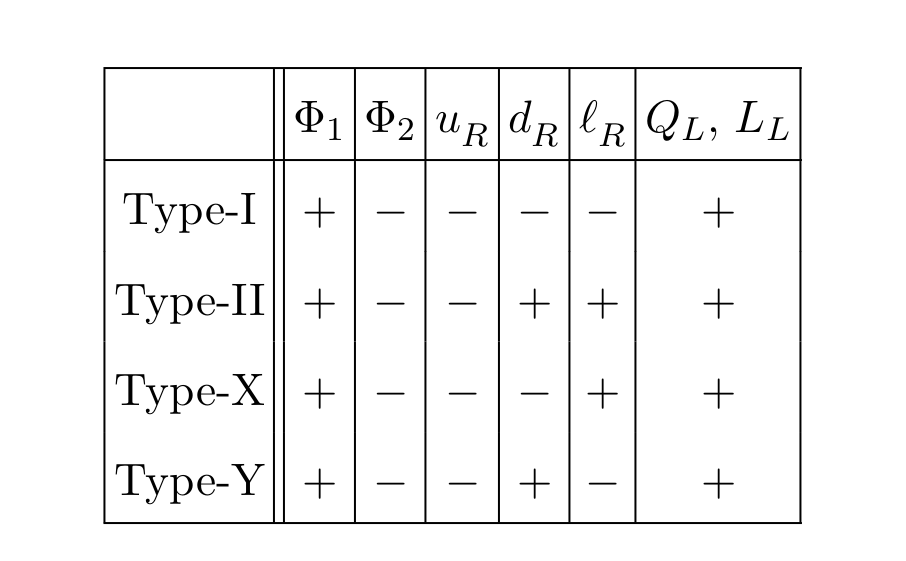
\includegraphics[scale= 0.8]{../Cap1/2hdm}
\caption{Variation in charge assignments of the $Z_2$ symmetry.}
\label{2hdm}
\end{figure}
 In the type-I, all quarks and charged leptons obtain their masses from the VEV of $\Phi_2$.  
In the type-II, masses of up-type quarks are generated by the VEV of  $\Phi_2$, while those of down-type quarks and charged leptons are acquired by that of  $\Phi_1$.The Higgs sector of the MSSM is a special 2HDM whose Yukawa interaction is of type-II. The type-X Yukawa interaction (all quarks couple to  $\Phi_2$ while charged leptons couple to  $\Phi_1$) is used in the model described in~\cite{PhysRevD.80.015017}. The remaining one is referred to as the type-Y.
The most general Higgs potential under the  broken $Z_2$ symmetry is given by,
\newline
\begin{equation}
\begin{split}
V^{2HDM}=& m_1^2 \Phi_1^{\dag}\Phi_1 +m_2^2 \Phi_2^{\dag}\Phi_2 -m_3^2(\Phi_1^{\dag}\Phi_1 +  \Phi_2^{\dag}\Phi_2) +\frac{\lambda_1}{2}(\Phi_1^{\dag}\Phi_1)^2  \\
&+\frac{\lambda_2}{2}(\Phi_2^{\dag}\Phi_2)^2  +\lambda_3 (\Phi_1^{\dag}\Phi_1 +  \Phi_2^{\dag}\Phi_2) +\lambda_4 (\Phi_1^{\dag}\Phi_2 +  \Phi_2^{\dag}\Phi_1)  \\
&+\lambda_5 [(\Phi_1^{\dag}\Phi_2)^2 + (\Phi_2^{\dag}\Phi_1)^2] \; , \end{split} \end{equation}
\newline
where the parameters $m_3^2$ and $\lambda_5$ are complex, in general but in the following , assuming CP invariance, they are real.
The Higgs doublet fields can be parametrized as,
\newline
\begin{equation}
\Phi_i=
\left(
\begin{array}{c}
\omega_i^+   \\
\frac{1}{\sqrt{2}}(v_i +h_i+ iz_i) \\
\end{array}
\right)
\;, \end{equation}
and the mass eigenstates are defined by,
\newline
\begin{equation}
\begin{split}
\left(
\begin{array}{c}
h_1   \\
h_2 \\
\end{array} 
\right) &= R(\alpha)
\left(
\begin{array}{c}
H   \\
h \\
\end{array}
\right)\:, \qquad \\
\\
\left(
\begin{array}{c}
z_1   \\
z_2 \\
\end{array} 
\right) &= R(\beta)
\left(
\begin{array}{c}
z   \\
A \\
\end{array}
\right)\:, \qquad \\
\\
 \left(
\begin{array}{c}
\omega_1^+   \\
\omega_2^+ \\
\end{array}
\right) &= R(\beta)
\left(
\begin{array}{c}
\omega^+   \\
H^+ \\
\end{array}
\right)\:,  \end{split}
\end{equation}
\newline
where the rotation matrix is given by,
\begin{equation}
R(\theta)=
\left(
\begin{array}{lr}
\cos \theta & -\sin \theta   \\
\sin \theta & \cos \theta  \\
\end{array}
\right)
\;. \end{equation}
There are five physical Higgs bosons,  i.e., two CP-even states $h$ and $H$, one CP-odd state $A$
, and a pair of charged states $H^{\pm}$, while $z$ and $\omega^{\pm}$ are Nambu-Goldstone bosons that are eaten as the longitudinal components of the massive 
gauge bosons. The eight parameters, $m_i^2$ ($i=1,3$) and $\lambda_j$ ($j=1,5$) in the Higgs sector are replaced by eight physical parameters:
\begin{itemize}
\item the VEV $v=\sqrt{v_1^2+ v_2^2}$,
\item the mixing angles $\alpha$ and $\beta$ ($\tan \beta= v_1/V_2 $) with $\sin( \beta -\alpha)=1 $,
\item the boson masses $m_h, m_H,m_A,m_H^{\pm} \:$,
\item the soft breaking mass parameter, $M=m_3/\sqrt{\sin \beta \cos \beta}$.
\end{itemize}
For the successful electroweak symmetry breaking, a combination of quartic coupling constants should satisfy the condition of vacuum stability.
In addition one has also to take into account
bounds from perturbative unitarity to restrict parameters in the Higgs potential.
The top and bottom Yukawa coupling constants cannot be taken to
 large. The requirement $|Y_{t,b}< \pi|$  at the tree level can provide a milder constraint $0.4 <\tan \beta <91$.\\
The  wide  range  of  possibilities  for  Higgs  boson  mass  spectrum  hierarchies  and  branching
ratios  in  2HDMs  yields  a  diversity  of  production  and  decay  channels  that  are  relevant  for
multi-lepton  signatures  at  the  LHC.  Multi-lepton  final  states  become  especially  important
when the decay of one Higgs scalar to a pair of Higgs scalars or a Higgs scalar and a vector
boson is possible. 



\subsection*{The WW decay channel for high mass Higgs-like particles}
Let’s now concentrate on the $X \to WW$ channel, that is the  final state using in the following  for the high mass searches.
The two dominant production mechanisms of high mass SM-like Higgs boson are the
gluon-gluon fusion and Vector Boson Fusion,  Fig. \ref{prod}. 
The first one is the main mechanism for mass values below 1 TeV, above the VBF production mechanism become more and more important as $m_X$ increases.
\begin{figure}
\centering
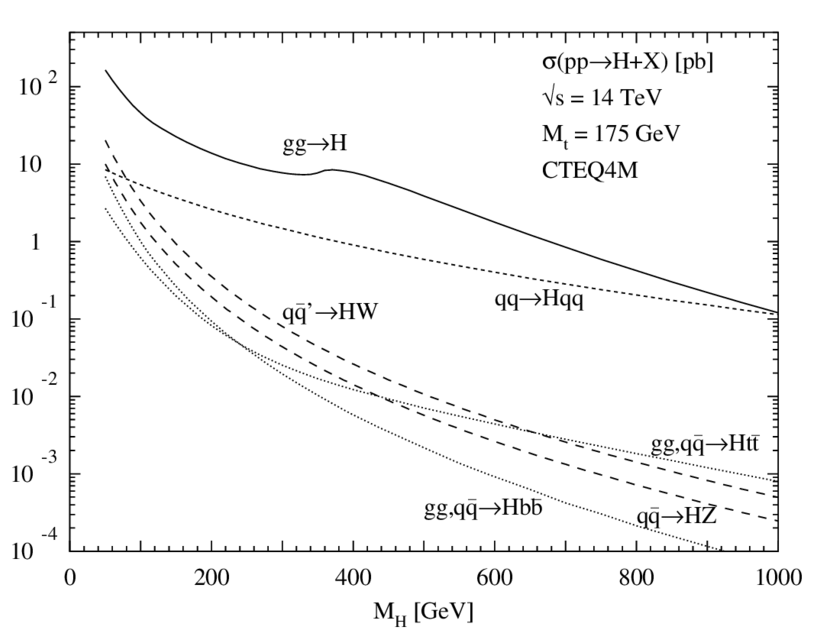
\includegraphics[scale= 0.4]{../Cap1/Higgs-production-cross-sections-at-the-LHC-for-various-production-mechanisms-as-a}
\caption{Higgs-production cross sections at the LHC for various production mechanisms as a function of the Higgs mass. QCD corrections are included except for Higgs bremsstrahlung~\cite{Djouadi2004}.}
\label{prod}
\end{figure}
In the search for high mass Higgs boson, in many models, the WW final state, along with ZZ, is the dominant decay channel of $X$ for masses above $2m_Z$ threshold. This fact is evident in Fig.~\ref{br}~(a), where the $WW$ branching ratio (in green) dominates in the high mass region. More detailed results on the decays $H \to WW$ and $H \to ZZ $ with the subsequent decay chain are presented in Fig.~\ref{br}~(b).
However even if the yield for the decay channels started by the $X \to WW$ decay is higher,  the
presence of neutrinos in the final state does not allow to have a complete reconstruction of the decay.
 This fact makes this channel very challenging. 
As we have already noticed, gluon-gluon fusion cross section  is between one
and two orders of magnitude larger than that of VBF for a wide range of Higgs masses.
Nevertheless, the VBF becomes competitive when the mass approaches to 1 TeV. 
Furthermore, in case of gluon-gluon production mechanism, in addition to the two lepton and two neutrinos, there are rarely one or more jets coming from initial state radiation, Sec.~\ref{ps}. 
The VBF production, providing two more jets (the VBF jets coming from the hadronization quarks from production) to the final
state, benefits from a highly reduced background with respect to the gluon-gluon production mode,
such that even if the VBF production mechanism has a branching ratio smaller than the
gluon-gluon fusion, a higher signal-to-noise ratio is expected.
\begin{figure}
\centering%
\subfigure[]%
{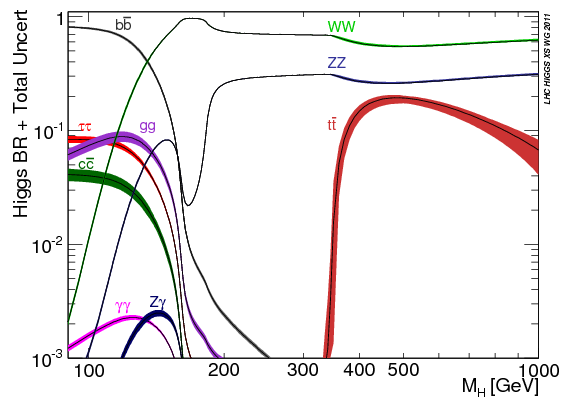
\includegraphics[scale= 0.6]{../Cap1/plots_decay}}
\subfigure[]%
{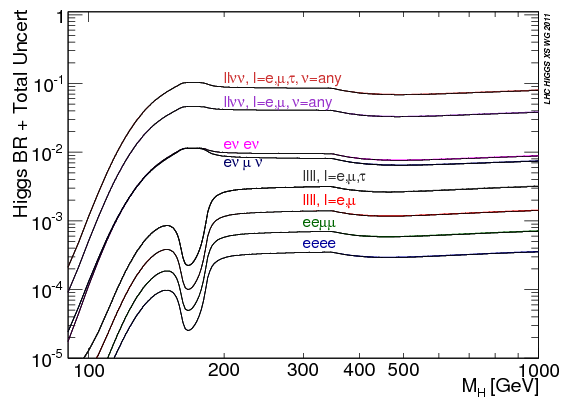
\includegraphics[scale= 0.6]{../Cap1/BRTotalUncertBands4f}}
\caption{(a) Higgs branching ratios and their uncertainties for the full mass range~\cite{Denner:2011mq}. (b) Higgs branching ratios for the different $H \to 4 \ell$ and $H \to 2\ell 2\nu $ final states and their uncertainties for the full mass range~\cite{Denner:2011mq}.}
\label{br}
\end{figure}



\subsection*{$X \to WW$ searches at colliders}
The search of high mass particle with  $WW$ final state  has been widely performed at experiments at hadron
colliders to search for new particles beyond the SM. 
The resonant $WW$ production has been studied at both the Fermilab Tevatron Collider, and the CERN Large
Hadron Collider, with the progressively increasing collision energy and integrated
luminosity. Each machine in its time has therefore probed the highest masses of
 resonances accessible. A review of the different searches
performed by D0, CDF, ATLAS and CMS, their techniques, data, results, and
limits on new particles decaying to $WW$ are described. 
%\paragraph{Searches at Tevatron} Before the Higgs boson discovery, the mass  searches for the high masses SM-like Higgs boson has been performed at the CDF
%and D0 detector, being the Higgs boson mass a free parameter. 
%These searches result in exclusions of the high mass range  156.5 $<m_H<$173.7 GeV for CDF and 161$<m_H<$170 GeV for D0~\cite{Petridis:2012jd}. 
%The high mass searches at CDF and D0 require at least one electron or a muon in the final state in order to suppress the QCD background. Given this requirement all possible decay  modes  are  considered  to  maximise  the  signal  acceptance. The di-lepton plus missing transvere energy channel requires two electrons or muons (plus neutrinos) of opposite charge in the final state. This represents a small WW decay branching ratio, but a clean signature offering the highest sensitivity  of  all  the  high  mass  channels. 
%CDF and D0 set limits by combining all of the SM high mass channels with up to 8.2 fb$^{-1}$of integrated luminosity.
%\begin{figure}
%\centering
%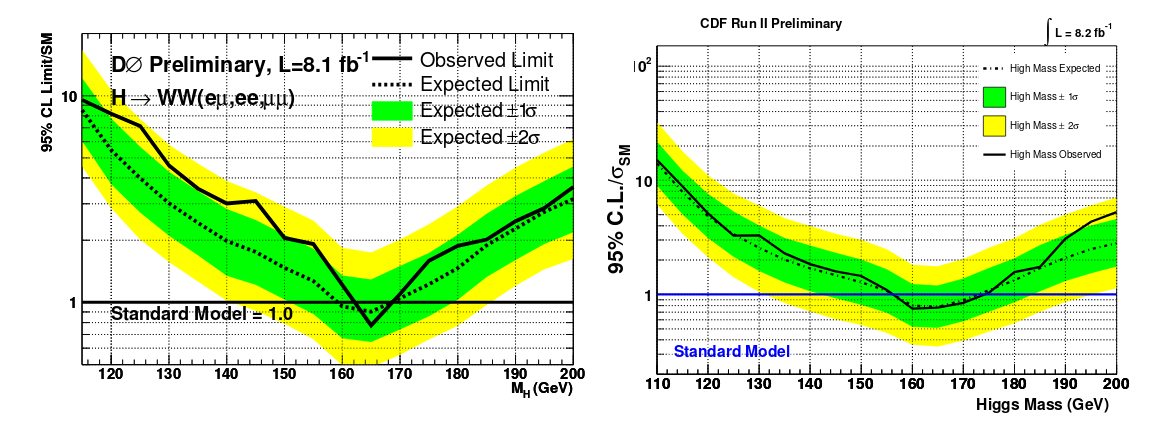
\includegraphics[scale= 0.33]{../Cap1/tevatron}
%\caption{Combined limits using the di-lepton channels for D0 (left) and CDF (right).}
%\label{tevatron}
%\end{figure}
%\paragraph{Searches at LHC} 
After the discovery of the Higgs boson at LHC, the two experiments, ATLAS and CMS, have been focused on high mass searches using the data collected at $\sqrt{s}=$7, 8 (Run-I) and 13 TeV (Run-II). A search for a heavy Higgs boson in the $H \to WW$ and $H \to ZZ$ decay channels has been performed by the
CMS experiment based on  proton-proton collision data samples corresponding to an integrated luminosity of up to 5.1 $fb^{-1}$ at $\sqrt{s}=7$ TeV and up to 19.7  $fb^{-1}$ at $\sqrt{s}=8$~\cite{Khachatryan:2015cwa}. This analysis is performed in a mass range 145 < $m_H$ < 1000 GeV and searches for a heavy Higgs boson in the EW singlet extension of the SM. The peculiarity of this analysis is that the full Run-I statistics is considered and the mass range reach 1 TeV for the first time in CMS.
In the case of a high Higgs boson decaying into a pair of W bosons, the fully leptonic ($X \to WW \to 2\ell 2\nu$) and semileptonic ($X \to WW \to \ell \nu qq$) final
states are considered in this  analysis. 
Decays containing four charged leptons  ($X \to WW \to 2\ell 2\ell'$), two charged leptons and two quarks ($X \to ZZ \to \ell \nu qq$) and two charged leptons and two neutrinos ($X \to ZZ \to 2\ell 2\nu$) are considered. No significant excess over the expected
SM background has been observed and exclusion limits have been set. The combined results obtained for a heavy Higgs boson with SM-like couplings for all
the different contributing final states are displayed in Fig.~\ref{plots_combination_combinedSM_def}. On the left, the observed
95\% CL limit is shown for each final state. On the right, the expected and observed limits are
displayed for each of the individual channels as well as the combined result.
\begin{figure}
\centering
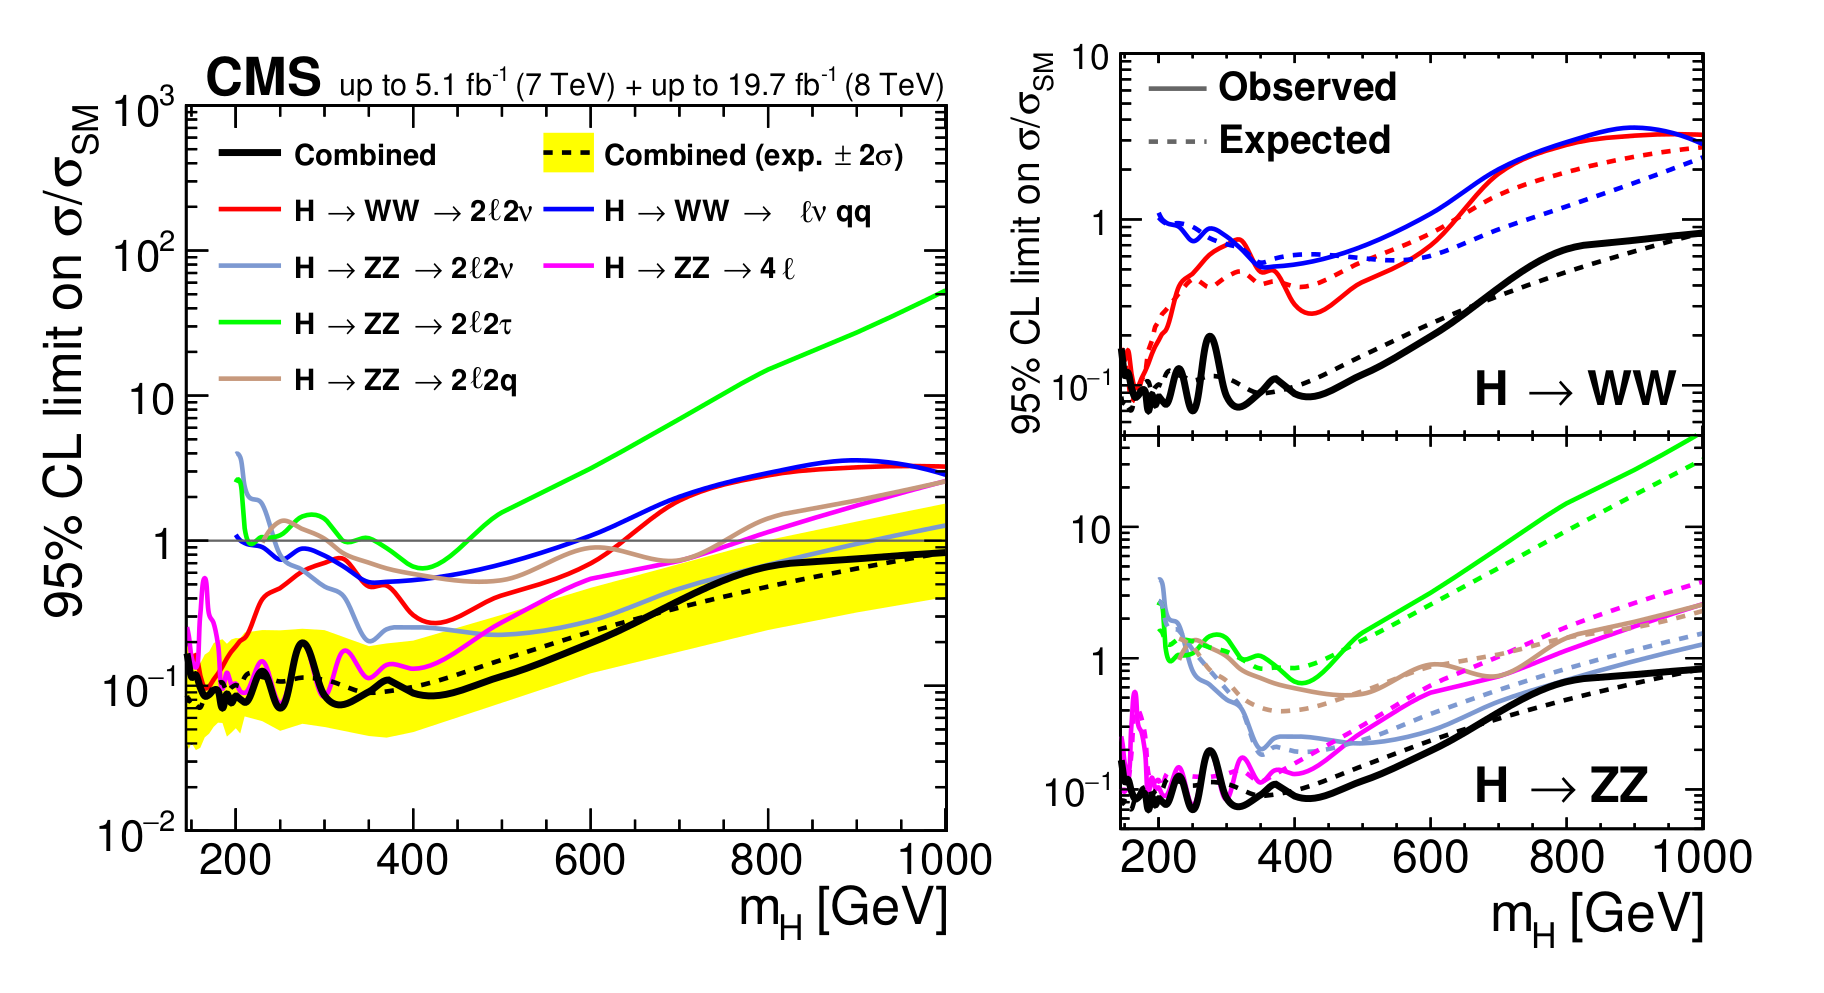
\includegraphics[scale= 0.9]{../Cap1/plots_combination_combinedSM_def}
\caption{Upper limits at the 95\% CL for each of the contributing final states and their combination.  ~\cite{Khachatryan:2015cwa}. }
\label{plots_combination_combinedSM_def}
\end{figure}
Using the 13 TeV proton-proton collision data produced at the LHC in 2015, corresponding to an integrated luminosity
of 2.3 fb$^{-1}$, CMS has  performed the search for a final state with different flavour leptons ($X \to WW \to 2\ell 2\nu$) in the mass range  200$< m_H< 1000$ GeV~\cite{CMS-PAS-HIG-16-023}. The search has been carried out in the 0-jets, 1-jet and VBF categories in order to increase the signal sensitivity to different production mechanisms and maximize the exclusion limits. 
No significant excess with respect to the SM background expectation has been observed, and
the exclusion limits on the cross section times branching ratio to  $ WW \to 2\ell 2\nu$ ave been reported, Fig.~\ref{lim_2015}
\begin{figure}
\centering
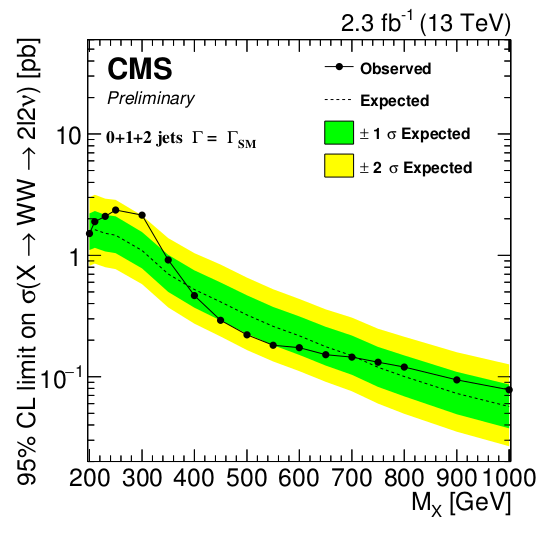
\includegraphics[scale= 0.4]{../Cap1/lim_2015}
\caption{Expected and observed exclusion limits at 95\% CL on the sum of ggH and VBF cross
sections times branching fraction for the combination of the three jet categories as a function
of the resonance mass. The black dotted line corresponds to the central value while the yellow
and green bands represent the $\pm 1\sigma$ and $\pm 2\sigma$  uncertainties respectively. }
\label{lim_2015}
\end{figure}
The ATLAS collaboration published the results of a search for a heavy neutral scalar decaying to two $W$ bosons using the datasets collected in 2015 and early
2016 at a centre-of-mass energy $\sqrt{s}=$13 TeV corresponding to an integrated luminosity of 13.2 fb$^{-1}$ in the mass range between
300 GeV and 3 TeV~\cite{ATLAS-CONF-2016-074}. In this analysis, categories with one- and at least two-jets
are optimised for a vector boson fusion-like signal and the remaining category is quasi-inclusive
for a gluon-gluon fusion-like signal. The search sensitivity depends on the assumed Higgs boson width. Two different hypotheses are tested:
a narrow width approximation, where the width of the heavy Higgs boson is smaller than the
experimental resolution, and a large width assumption, where widths of 5\%, 10\%, and 15\% of
the heavy Higgs boson mass are considered.
Upper limits are set on  the production cross section times the $H \to WW$ branching ratio in two scenarios:
a high-mass Higgs boson with a narrow width, and  with intermediate widths (of 5, 10, 15\% of the
heavy Higgs boson mass), Fig.~\ref{ATLAS-CONF-2016-074_fig}. Values above 4.3 pb (1.4 pb) at $m_H=$300 GeV (400 GeV) and above 0.051 pb
(0.071 pb) at 3 TeV are excluded at 95\% CL by the gluon-gluon fusion quasi-inclusive NWA (LWA 15\%) analysis. For
the VBF NWA case, the upper exclusion limit ranges between 1.1 pb at $m_H=$ 300 GeV to 0.03 pb at 3 TeV.

\begin{figure}
%\centering
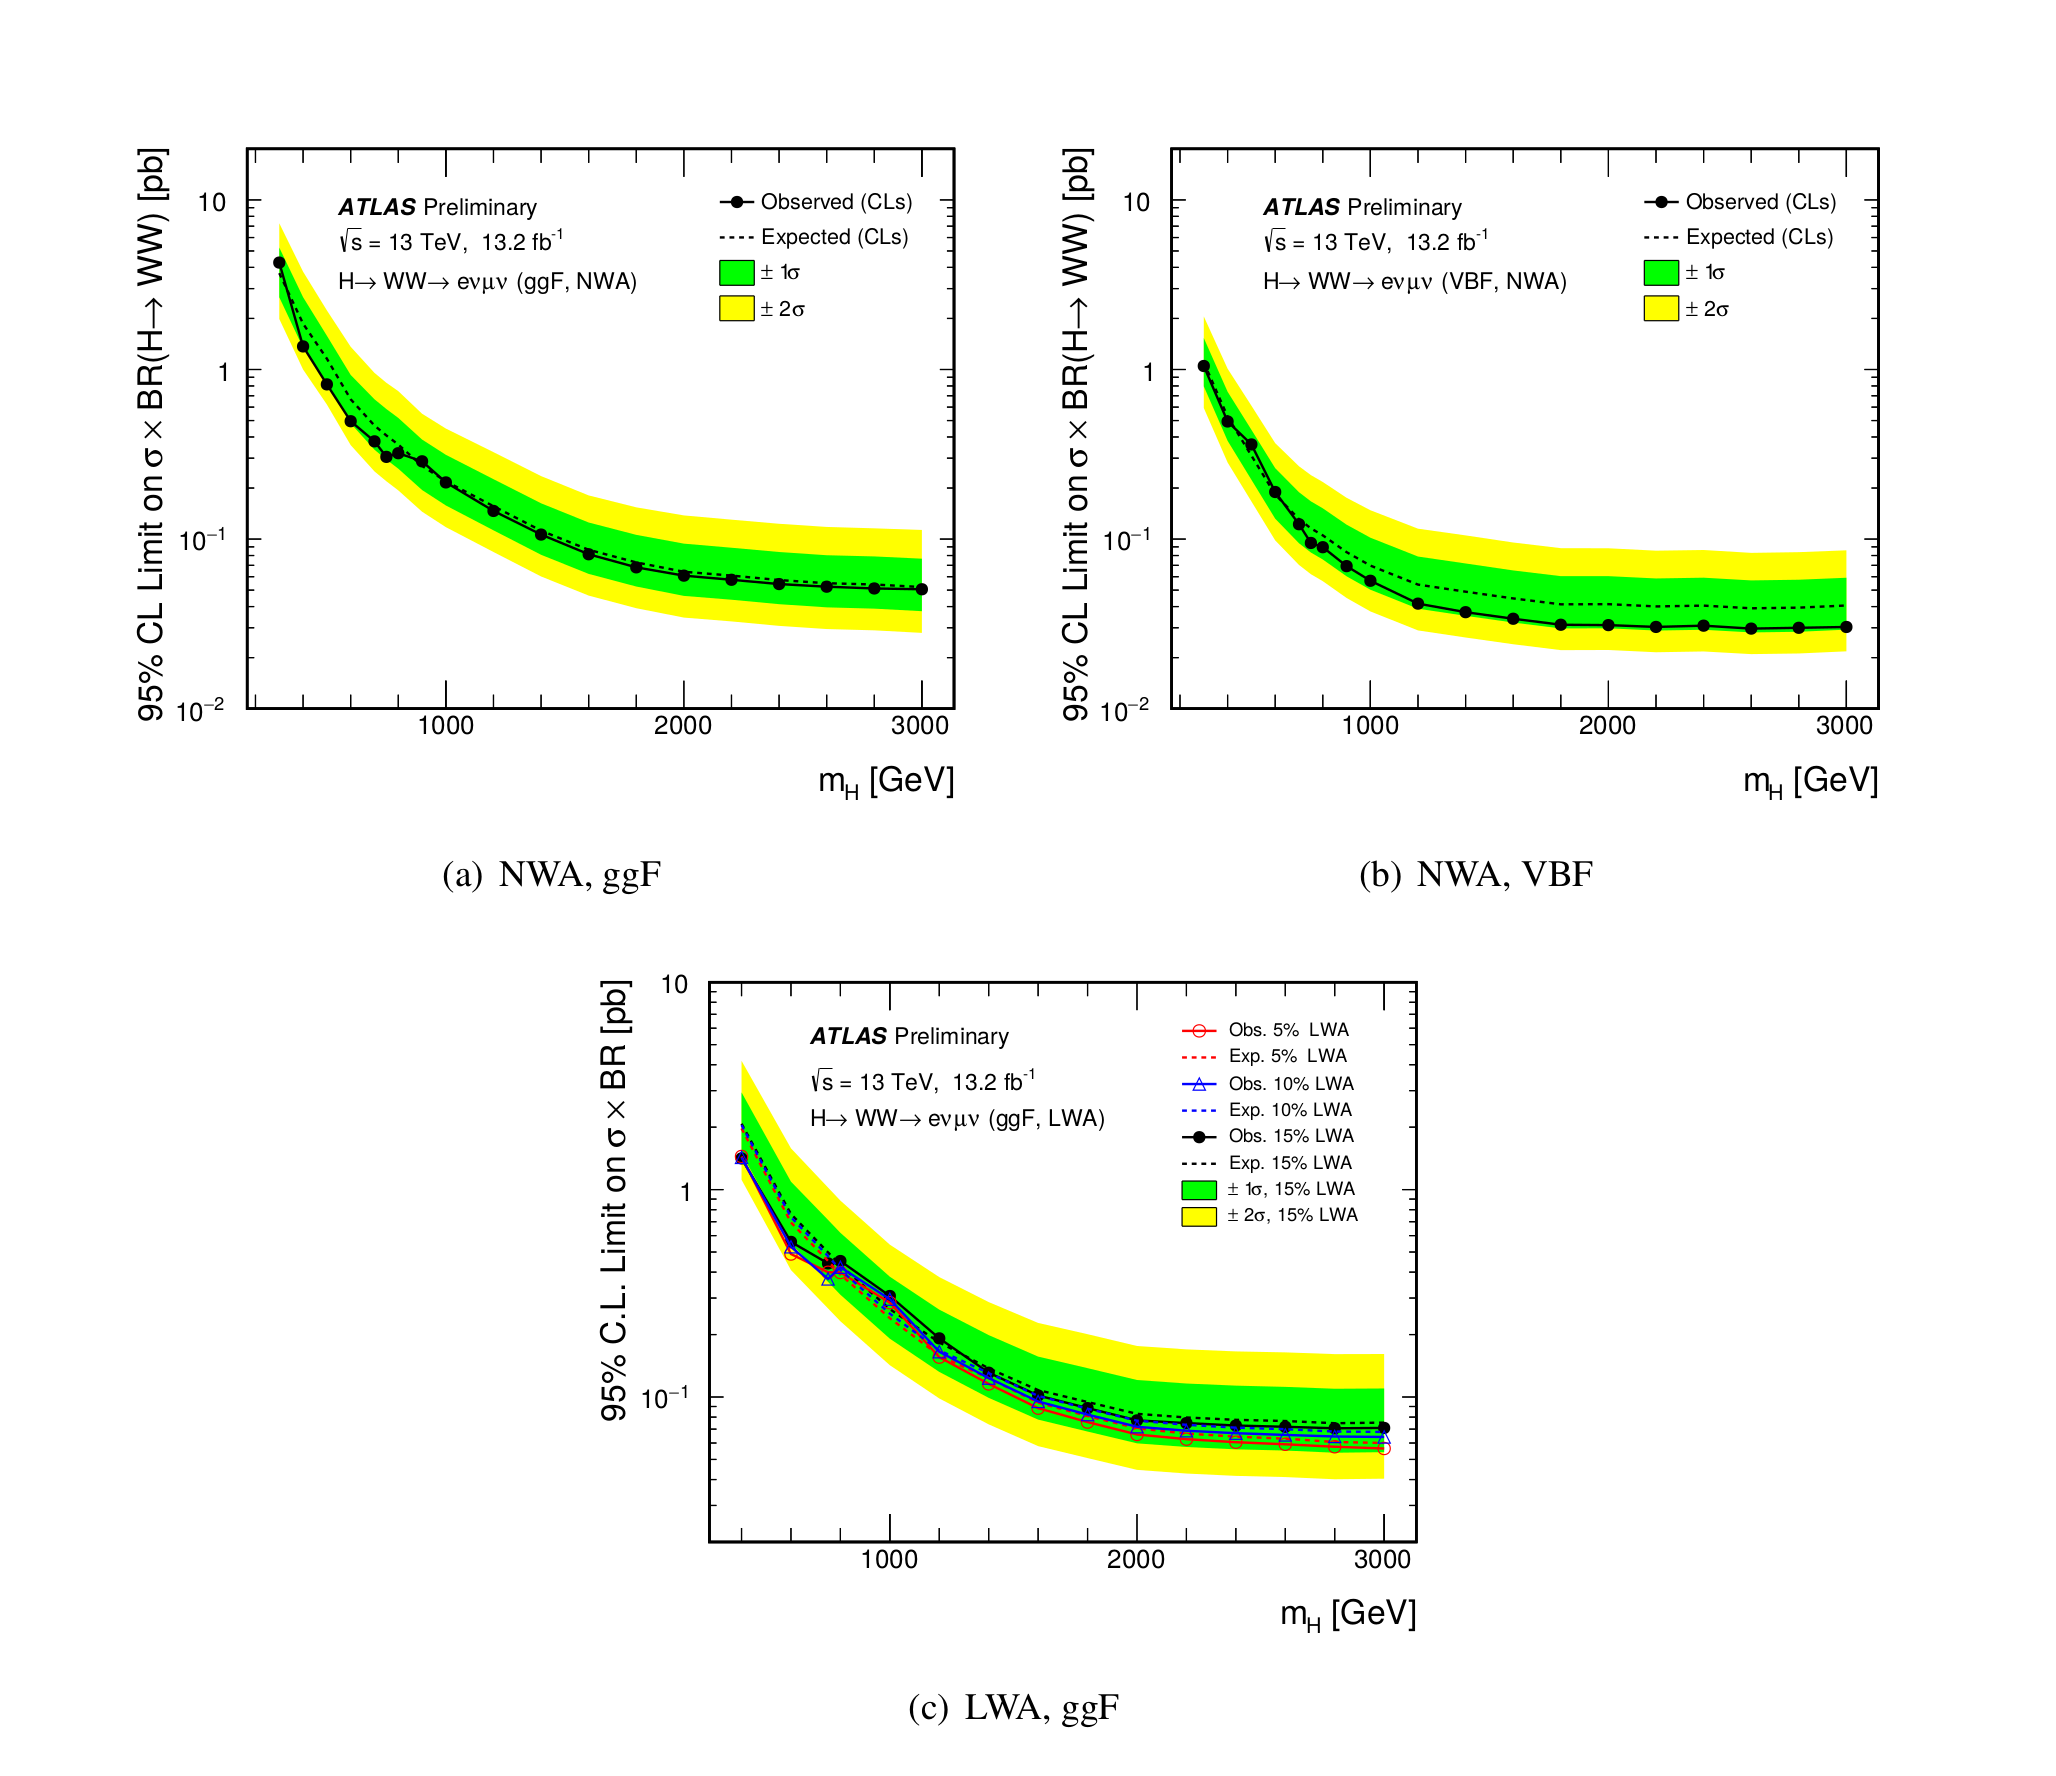
\includegraphics[scale= 0.9]{../Cap1/ATLAS-CONF-2016-074}
\caption{95\% CL upper limits on the Higgs production cross section times branching ratio in the analysis, for signals with narrow-width (gluon-gluon fusion or VBF) in the top row and the 5\%, 10\% and 15\% width lineshapes (gluon-gluon fussion only) in the bottom. The green and yellow bands show the  $\pm 1\sigma$ and  $\pm 2\sigma$ uncertainties on the expected limit. }
\label{ATLAS-CONF-2016-074_fig}
\end{figure}
} 
{\chapter{The CMS experiment at LHC}

\section{The Large Hadorn Collider}
The Large Hadron Collider (LHC)~\ref{Pettersson:291782}  at CERN,  on 2008, is the largest and most powerful hadron collider ever built. Installed in the
underground tunnel which housed the Large Electron Positron Collider (LEP),
the leptonic accelerator in operation until 2nd November 2000, the LHC accelerator has
the shape of a circle with a length of about 27 km and is located at a depht varying
between 50 m to 175 m, straddling the Franco-Swiss border near Geneva. It is designed
to collide two 7 TeV counter-circulating beams of protons resulting in a center-of-mass
energy of 14 TeV, or two beams of heavy ions, in particular lead nuclei at an energy of
2.76 TeV/nucleon in the center-of-mass frame.
The transition from a leptonic collider to a hadronic collider entailed the following
advantages: first, it has been possible to build a machine that having the same size of the
previous one (and therefore accommodated in the same LEP tunnel, substantially reduc-
ing the cost and time of construction), could reach a higher energy in the center-of-mass
frame. This is due to the much lower amount of energy loss through synchrotron radiation
emitted by the accelerated particles, that is proportional to the fourth power of the ratio
E/m between their energy and their mass. Secondly, the composite structure of protons
compared to the elementary structure of electrons allows LHC to be able to access simultaneously a wider energy spectrum, despite the production of many low energies particles in a complex environment. This feature is particularly important for a machine dedicated
to the discovery of “new” physics.
Schematic description of the accelerator complex installed at CERN is shown in Fig.~\ref{lhc}
The acceleration is performed in several stages. The protons source is a Duoplasma-
tron: the protons are obtained by removing electrons from a source of hydrogen gas
and then sent to the LINAC2, a 36 m long linear accelerator which generates a pulsed
beam with an energy of 50 MeV using Radio Frequency Quadrupoles (RFQ) and focusing
quadrupole magnets. The beam is subsequently sent to the Proton Synchrotron Booster
(PSB), a circular accelerator consisting of four superimposed synchrotron rings with a
circumference of about 160 m, which increases the proton energy up to 1.4 GeV. Then,
protons are injected into the Proton Synchrotron (PS), a single synchrotron ring with a
circumference of about 600 m where the energy is increased to 25 GeV. The sequential combination of these two synchrotrons also allows to create a series of protons bunches
interspersed by 25 ns (i.e. at the frequency of 40 MHz) as required for the final correct
operation of LHC. The final proton injection stage is the Super Proton Synchrotron (SPS),
a synchrotron with a circumference of approximately 7 km where protons reach an energy
value of 450 GeV. Subsequently, protons are extracted and injected into the LHC ring
via two transmission lines, to generate two beams running in opposite directions in two
parallel pipes and which are accelerated up to the energy of interest. The beams collide
at four interaction points where the four main experiments: ALICE, ATLAS, CMS and LHCb. Two small experiments, TOTEM and LHCf, which focus on forward particles, have also been built.
The 7 TeV per-beam-energy limit on the LHC
is not determined by the electric field generated by the radiofrequency cavity but by the
magnetic field necessary to maintain the protons in orbit, given the current technology
for the superconducting magnets.
\begin{figure}
\centering
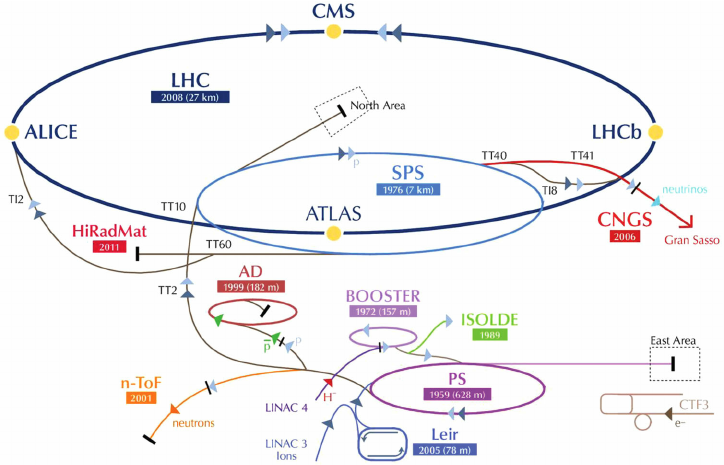
\includegraphics[scale= 0.5]{../Cap2/lhc}
\caption{Schematic description of the accelerator complex installed at CERN.}
\label{lhc}
\end{figure}
One of the most important parameter of an accelerator is the instantaneous luminosity $\mathcal{L}$. For a process having a cross section $\sigma$ and producing N particles per time unit, the
instantaneous luminosity $\mathcal{L}$ is defined by the relation
\begin{equation}
N= \mathcal{L} \sigma \end{equation}
Then the integrated luminosity $L$ can be defined as
\begin{equation}
L=\int \mathcal{L}  dt \end{equation}


\section{The Compact Muon Solenoid experiment}
The Compact Muon Solenoid (CMS)  is a general purpose detector optimized for the
proton-proton interactions analysis with the expected energy and luminosity of the LHC
particle accelerator design, identifying with precision muons, electrons and photons. It
has been designed to investigate a wide range of physics, with the search for the Higgs
boson as one of the main highlights. Search for new physics is also an important goal of the
experiment, as well as top physics and, of course, Standard Model precision measurements.
Although it has the same scientific goals as the ATLAS experiment, it uses different
technical solutions and a different magnet-system design. The CMS experiment is one
of the largest international scientific collaborations in history, involving more than 4000
people (particle physicists, engineers, technicians, students and support staff) from about
180 universities and institutes in more than 40 countries.
The experiment is placed in a cavern 100 m underground in the area called Point 5 (an old LEP access point) near the village of Cessy, in France.
The coordinate system used in CMS is a right-handed Cartesian system, having the origin
in the nominal beam collision point inside the detector. The x-axis points radially towards
the center of the LHC ring, the y-axis is directed upwards along the vertical and the z-
axis is oriented along the direction of the beams, along the counter-clockwise direction of
the ring if seen from above. The cylindrical symmetry of CMS design and the invariant
description of proton-proton physics suggest to define a new coordinate system based on
pseudo-angular coordinates, given by the triplet ($r$, $\phi$, $\eta$) where $r$ is the distance from
the $z$-axis, $\phi$ is the azimuth angle measured on the $x-y$ plane starting from the $x$-axis
and $\eta$ is the pseudorapidity, App.~\ref{psr}.\\
\newline
The CMS detector,  Fig.~\ref{cms}, is 21.6 m long, has a diameter of 15 m and a
weight of about 12, 500 tons. The constructive element that characterizes the experiment
is a solenoidal superconducting magnet which produces an internal constant magnetic
field of 3.8 T along the direction of the beams. The CMS detector is designed as a
dodecagonal base prism. The central part of the prism, named barrel, contains several
layers of detectors with cylindrical symmetry, coaxial with respect to the direction of the
beams. A set of detector disks, called endcaps, close the detector at its ends, to ensure its
tightness. 
\begin{figure}
\centering
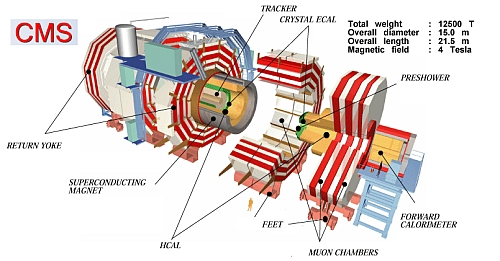
\includegraphics[scale= 1]{../Cap2/cms}
\caption{A view of the CMS detector with its subdetectors labeled.}
\label{cms}
\end{figure}
From the inner region to the outer one, the various components of CMS are:
\begin{itemize}
\item Silicon Tracker: it is placed in the region $r$ < 1.2 m and $|\eta|$ < 2.5. It consists of
a silicon pixel vertex detector and a surrounding silicon microstrip detector, with a
total active area of about 215 m$^2$ . It is used to reconstruct charged particle tracks
and vertices;
\item Electromagnetic Calorimeter (ECAL): it is placed in the region 1.2 m $< r <$
1.8 m and $|\eta|$< 3. It consists of scintillating crystals of lead tungstate  and it is used to measure the trajectory and the energy released by photons and
electrons;
\item Hadron Calorimeter (HCAL): it is placed in the region 1.8 m $< r <$ 2.9 m and
$|\eta|$ < 5. It consists of brass layers alternated with plastic scintillators and it is used
to measure the direction and the energy released by the hadrons produced in the
interactions;
\item Superconducting Solenoidal Magnet: it is placed in the region 2.9 m $< r <$
3.8 m and  $|\eta|$< 1.5. It generates an internal uniform magnetic field of 3.8 T along
the direction of the beams, necessary to deflect the charged particles in order to
allow a measurement of their momentum through the curvature observed in the
tracking system. The magnetic field is closed with an iron yoke 21.6 m long with a
diameter of 14 m, where a residual magnetic field of 1.8 T is present, in the opposite
direction with respect to the 3.8 T field;
\item Muon System: it is placed in the region 4 m $< r < 7.4$ m and $|\eta|$ < 2.4. It consists
of Drift Tubes (DT) in the barrel region and Cathode Strip Chambers (CSC) in the
endcaps. A complementary system of Resistive Plate Chambers (RPC) is used both
in the barrel and in the endcaps. This composite tracking system for muons is used
to reconstruct tracks released by muons that pass through it. The muons chambers
are housed inside the iron structure of the return yoke that encloses the magnetic
field.
\end{itemize}

\subsection*{The Tracker}
The silicon tracker is the detector closest to the beams collision point. Its goal is
the high resolution reconstruction of the trajectories of charged particles originating
from the interaction point and the identification of the position of secondary vertices
produced by particles with a short mean life time (in particular hadrons containing the
b quark, that decay after few hundreds of $\mu$m). The events produced in the proton-
proton collisions can be very complex and track reconstruction is an involved pattern
recognition problem. Indeed, at the nominal instantaneous luminosity of operation,
an average of about 20 pile-up events overlapping to the event of interest are expected,
leading to about 1000 tracks to be reconstructed every 25 ns. In order to make the
pattern recognition easier, two requirements are fundamental:
a low occupancy detector and a large redundancy of the measured points (hits) per track.
The first requirement is achieved building a detector with high granularity 3 . The
redundancy of the hits is instead achieved having several detecting layers, and is
necessary to reduce the ambiguity on the assignment of the hits to a given track.
Nevertheless, the amount of tracker material has to be as low as possible, in order to
avoid compromising the measurement of the particle trajectory. An excessive amount
of material would indeed deteriorate the measurement, mainly because of the increased
probability of particle multiple scattering. The outer detectors such as ECAL would
be influenced by the material as well, for example because of the increased probability
for a photon to convert to an electron-positron pair in the tracker material. For this
reasons, the tracker layers are limited in number and thickness. The tracker comprises
a large silicon strip detector with a small silicon pixel detector inside it. In the central
$\eta$ region, the pixel tracker consists of three co-axial barrel layers at radii between
4.4 cm and 10.2 cm and the strip tracker consists of ten co-axial barrel layers extending
outwards to a radius of 110 cm. Both subdetectors are completed by endcaps on either
side of the barrel, each consisting of two disks in the pixel tracker, and three small
plus nine large disks in the strip tracker. The endcaps extend the acceptance of the
tracker up to $|\eta|$ < 2.5. A three-dimensional schematic view of the tracker is shown in
Fig.~\ref{trk}, while in Fig.~\ref{fig_cmstracker} a pictorial representation of a slice of the tracker is displayed,
showing the various layers of the subdetectors.
The whole tracker has a cylindrical shape with a length of 5.8 m and a diameter
of 2.5 m, with the axis aligned to the beams direction. The average number of hits
per track is 12-14, allowing high reconstruction efficiency and low rate of fake tracks.

\begin{figure}
\centering
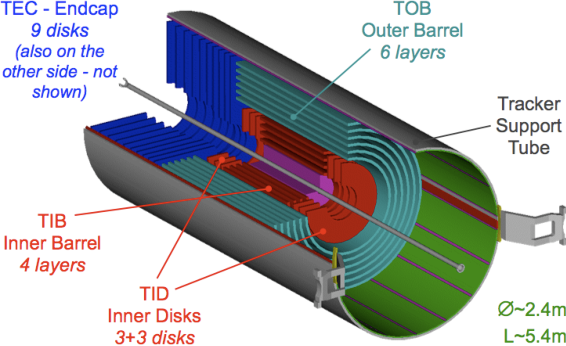
\includegraphics[scale= 0.5]{../Cap2/trk}
\caption{Three-dimensional schematic view of the CMS silicon tracker.}
\label{trk}
\end{figure}

\begin{figure}
\centering
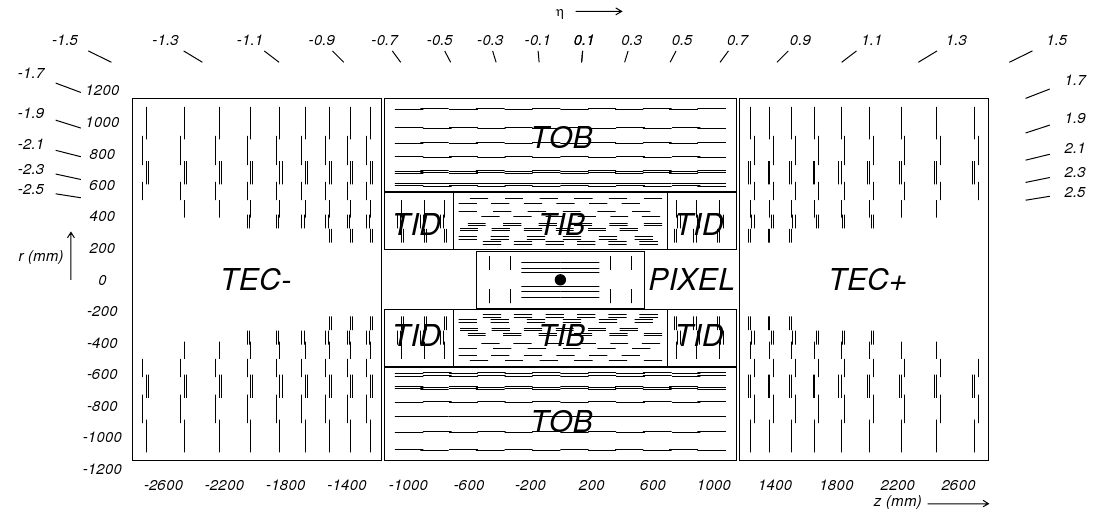
\includegraphics[scale= 0.3]{../Cap2/fig_cmstracker}
\caption{Pictorial view of a tracker slice in the r-z plane. Pixel modules are shown in
red, single-sided strip modules are depicted as black thin lines and strip stereo modules are
shown as blue thick lines.}
\label{fig_cmstracker}
\end{figure}

\paragraph*{The Pixel Vertex Detector} The pixel vertex detector,  is mainly used in CMS as a starting point for
the reconstruction of tracks and is essential for the reconstruction of the primary vertex
(PV) and any possible secondary vertices. It is placed in the region closest to the collision
point, where the particle flow is maximum. It covers the region $|\eta|$ < 2.5 and is composed
of a central part (barrel) and by two forward parts (endcaps). The barrel is composed of
three concentric cylindrical sectors 53 cm long, located at an average distance r of 4.4 cm,
7.3 cm and 10.2 cm. Each half-cylinder is composed of ladders and half ladders that serve
as support and cooling structure for the modules of pixels, with each ladder containing 8
modules. In total, the barrel is composed of 768 modules. Each endcap is composed of
two disks placed at a distance of 34.5 cm and 46.5 cm from the nominal beams impact
point. They cover a radius $r$ in a range between 6 cm and 15 cm in such a way that each
track included in the detector acceptance passes through at least two layers. Each disk is
divided into 24 segments, on each of which 7 modules of different sizes are mounted, for
a total of 672 modules on all the endcaps. Each module is composed of several units that
contain a highly integrated and segmented silicon sensor with a thickness of 250 $\mu$m. In
order to optimize the reconstruction of vertices and the track parameters near the vertex,
a set of rectangular pixels with a size of 150 × 100 $\mu$m 2 are used, with the 100 $\mu$m side
oriented along the $r \phi$ direction in the barrel region and along the $z$ direction in the endcap
region. The resolution in the hit reconstruction is about 10-15 $\mu$m in the barrel and
about 15 $\mu$m in the endcaps.

\paragraph*{The Silicon Microstrip Detector} In the region of the detector that is more than 20 cm far from the beam, the flow of
particles is sufficiently limited to allow the use of a silicon microstrip detector (Silicon
Strip Tracker, SST). Overall, this detector consists of 15400 units (modules), composed
of one or two sensors sticked on a support of carbon fiber, together with the readout
electronics. In case of a “doubled” sensor, the second detector is rotated with respect
to the first one in order to have strips forming an angle of 100 mrad between them.
This “stereo” combination, although of lower resolution, is preferable compared to a pixel segmentation because it has a lower number of readout channels. 
The ambiguities due to
the hit recognition are resolved in the process of reconstruction of the entire track. The
silicon microstrip tracker is 5.4 m long, extending up to a distance of 1.1 m from the axis
of the beams. It consists of a barrel and two endcaps and it is divided into four distinct
parts, TIB and TOB, and TID and TEC.


\subsection*{The Electromagnetic Calorimeter (ECAL)}
The main function of an electromagnetic calorimeter is to identify electrons and photons
and to measure accurately their energy. The electromagnetic calorimeter (Fig.~\ref{ecal_all} ) of
CMS (ECAL, Electromagnetic CALorimeter )  is a homogeneous calorimeter with
cylindrical geometry, whose elements are scintillating crystals of lead tungstate (PbWO$_4$)
with a truncated pyramidal shape. It consists of an ECAL Barrel (EB) with 61200 crystals
and two ECAL Endcaps (EE) containing 7324 crystals each one.
Crystals are grouped into 5 × 5 matrices called towers. The barrel has an inner radius of
129 cm, a length of 630 cm and it extends in the region $|\eta|$ < 1.479. Crystals in the ECAL
barrel have the following dimensions: 22 × 22 mm$^2$ at the front face, 26 × 26 mm$^2$ at the
rear face, and a length of 23 cm, corresponding to 25.8 $X_0$ . Each submodule, consisting
in a 5 × 2 crystals arrays mounted on a glass fiber structure, forms the elementar unit of
EB. The granularity of a single crystal is about 1 grade. To avoid that cracks might align with
particle trajectories, the crystal axes are tilted by 3 grade with respect to the direction from
the interaction point, both in the $\eta$ and $\phi$ direction.
Each endcap covers the region 1.479 < $|\eta|$ < 3 and is formed by two semicircular halves
of aluminum called dees. Crystals in endcaps have a length of 22 cm and frontal area
equal to 28.6 × 28.6 mm$^2$ . They are arranged in supercrystals with 5 × 5 elementary unity.
Unlike the crystals in the barrel, arranged in a $\eta - \phi $ symmetry, the endcap crystals are
arranged according to a $xy$ geometry.
Two preshower detectors are placed in front of the endcaps in order to separate the
showers produced by a primary $\gamma$ from those produced by a primary $\pi_0$ . This detector,
which covers the region 1.653 <  $|\eta|$ < 2.6, is a sampling calorimeter and it consists of two
disks of lead converters  that start the electromagnetic
shower of the incident photon/electron, alternating with two layers of silicon microstrip
detectors in which a measurement of the released energy and the identification of the
shower profile are performed. The strips are arranged orthogonally in the two planes,
according to a $xy$ configuration.
\begin{figure}
\centering
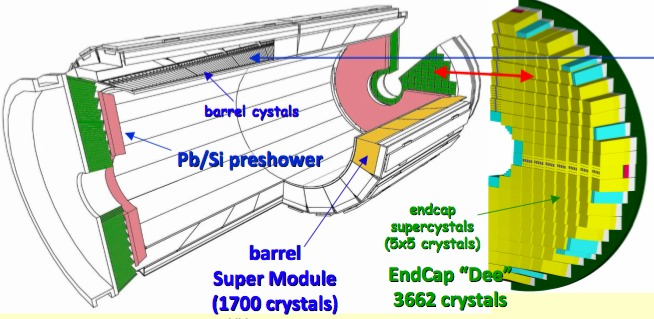
\includegraphics[scale= 0.5]{../Cap2/ecal_all}
\caption{Schematic representation of the electromagnetic calorimeter ECAL.}
\label{ecal_all}
\end{figure}
The choice of the PbWO$_4$ crystals as scintillating material for ECAL is due to several
reasons. First, the high-density the short radiation length  and the reduced Molière radius 5 (R M = 2.2 cm) allow to build a compact and
high granularity calorimeter. Furthermore, the 15 ns decay scintillation time allows to
collect about 80\% of the emitted light during the 25 ns that exist between two consecutive
beam interactions in the LHC design performance. Finally, the PbWO$_4$ crystals have a
good intrinsic radiation hardness and therefore they can operate for years in the hard
LHC environment, with a modest deterioration in performance. The main disadvantage
of these crystals is the low light yield  which makes an internal
amplification for the photodetectors necessary. This is achieved through the use of silicon
avalanche photodiodes  in barrel and single stage photomultipliers  in the endcaps, both resistant to the radiation and to the strong
magnetic field of CMS.
The energy resolution of a homogeneous calorimeter is usually expressed by the sum
in quadrature of three terms, according to the formula,
\begin{equation}
\frac{\sigma_e}{E}=\frac{a}{\sqrt{E}} + \frac{b}{E} + c \; ,
\end{equation}
The stochastic term a is the dominant term at low energies: it includes the contribution
of statistical fluctuations in the number of photoelectrons generated and collected.
The noise term b includes contributions from the electronic noise, both due to the pho-
todetector and to the preamplifier, and from pileup events.
The constant term c, dominant at high energies, takes into account several contributions:
the stability of the operating conditions (in particular of temperature and voltage), the
presence of dead material in front of the crystals and the rear leakage of the electromag-
netic shower, the longitudinal non uniformity of the crystal light yield, the intercalibration
errors and the radiation damage of the crystals.
The ECAL barrel energy resolution for electrons in beam tests has been measured to: $a=2.8\%$ GeV$^{-1/2}$, $b=12\%$ GeV, $c$ 0.3\%, where the energy E is measured in GeV.

\subsection*{The Hadronic Calorimeter (HCAL)}
The hadronic calorimeter HCAL (Hadronic CALorimeter ), together with the electromagnetic calorimeter, 
makes a complete calorimetric system for the jet energy and
direction measurement. Furthermore, thanks to its tightness, it can provide a measurement 
of the features of non-interacting particles, such as neutrinos, by measuring the
missing energy deposited in the transverse plane, $E_T^{Miss}$ or MET. The CMS hadronic calorimeter is
a hermetic sampling calorimeter that covers the region $|\eta|$ < 5. As shown in Fig.~\ref{hcal},
it is divided into four subdetectors: HB (Barrel Hadronic Calorimeter ), located in the
barrel region inside the magnet, extending up to pseudorapidities  $|\eta|$ < 1.4; HE (Endcap
Hadronic Calorimeter ), situated in the endcaps region inside the magnet, extends in the
pseudorapidity region 1.3   $<|\eta|<$  3, partially overlapping the HB coverage; HO (Outer
Hadronic Calorimeter, also called tail-catcher, placed along the inner wall of the magnetic 
field return yoke, just outside of the magnet; HF (Forward Hadronic Calorimeter ),
a sampling calorimeter consisting of quartz fibers sandwiched between iron absorbers,
consisting of two units placed in the very forward region (3  $<|\eta|<$ 5) outside the magnetic coil. 
The quartz fibers emit Cherenkov light with the passage of charged particles
and this light is detected by radiation resistant photomultipliers.
In order to maximize particle containment for a precise missing transverse energy
measurement, the amount of absorber material was maximized, reducing therefore the
amount of the active material. Since HCAL is mostly placed inside the magnetic coil,
a non-magnetic material like brass was chosen as absorber. HB and HE are therefore
made with brass absorber layers interleaved with plastic scintillators (wavelength shifters,
WLS) coupled to transparent optical fibers, which transmit the light to the HPD (Hybrid
Photodiodes) photodetectors.
\begin{figure}
\centering
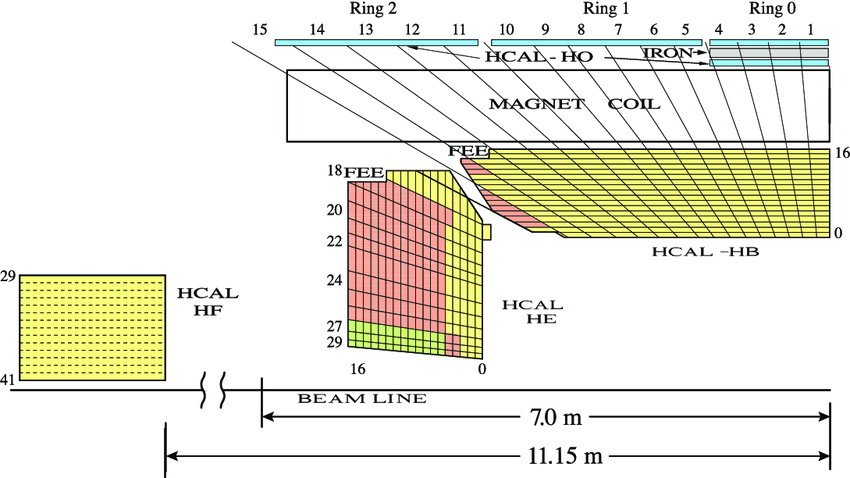
\includegraphics[scale= 0.4]{../Cap2/hcal}
\caption{A schematic $rz$ view of a quadrant of the CMS hadronic calorimeter HCAL.}
\label{hcal}
\end{figure}


\subsection*{The Solenoid Magnet}
The CMS magnet, which houses the tracker, the electromagnetic and the hadronic
calorimeters, is the biggest superconducting solenoid ever built in the world. The solenoid
achieves a magnetic field of 3.8 T in the free bore of 6 m in diameter and 12.5 m in length.
The energy stored in the magnet is about 2.6 GJ at full current. The superconductor is
made of four Niobium-Titanium layers. In case of a quench, when the magnet loses its
superconducting property, the energy is dumped to resistors within 200 ms. The magnet
return yoke of the barrel is composed with three sections along the z-axis; each one is
split into 4 layers (holding the muon chambers in the gaps). Most of the iron volume is
saturated or nearly saturated, and the field in the yoke is about the half (1.8 T) of the
field in the central volume.

\begin{figure}
\centering
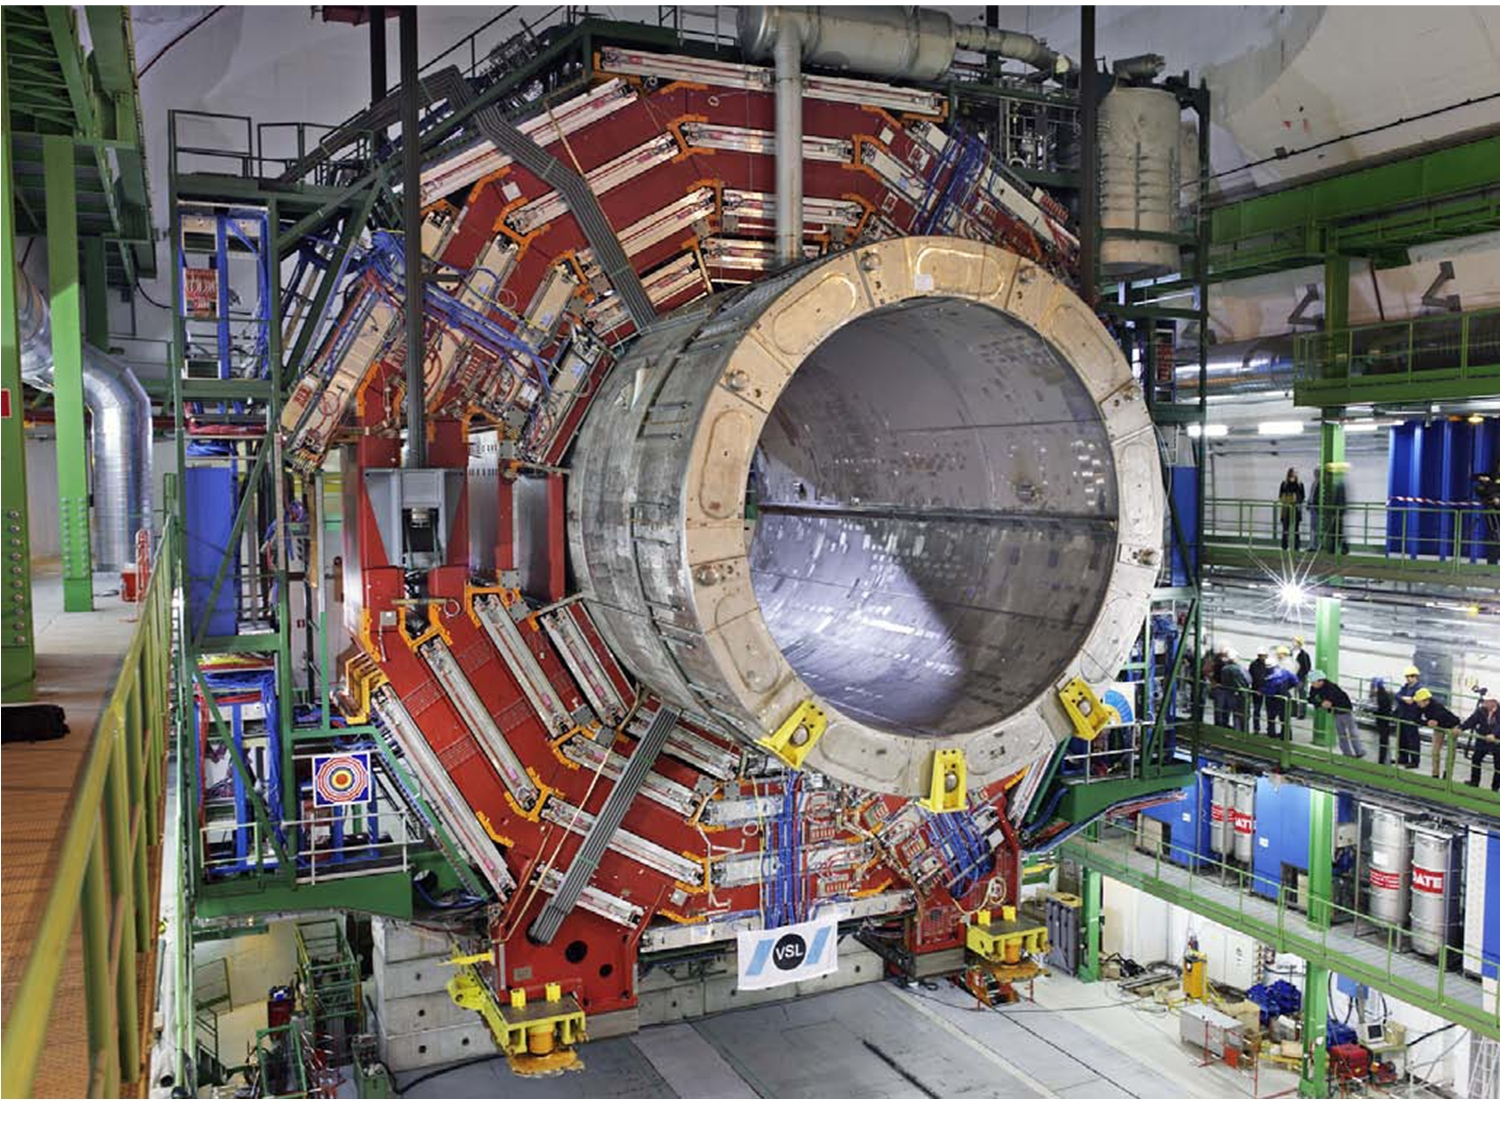
\includegraphics[scale= 0.35]{../Cap2/magnet}
\caption{Arrival of the magnet in the tunnel on February 28, 2007.}
\label{hcal}
\end{figure}

\subsection*{The Muon chamber}
The CMS Muon System  is dedicated to the identification and measurement of high
$p_T$ muons, in combination with the tracker. Furthermore, it provides a time measurement
of the bunch-crossing and also works as trigger for events involving muons. Momentum
measurement, in the muon system, is determined by the muon bending angle at the exit
of the 3.8 T coil, considering the interaction point as the origin of the muon. Up to $p_T$
values of 200 GeV, the resolution of the muon system is dominated by multiple scattering
and the best resolution is rather given by the silicon tracker, , Fig~\ref{muon_res}. The system is placed outside
the magnetic coil, embedded in the return yoke, to fully exploit the 1.8 T return flux. It
consists of three independent subsystems, as shown in Fig.~\ref{muon_c}: drift tubes (DT), cathode strip chambers (CSC) and resistive plate
chambers (RPC). The DT and the CSC provide an excellent spatial resolution for the
measurement of charged particle momentum; the RPC are used for trigger issues because
of the very good timing. The active parts of the muon system are hosted into stations
which are interleaved by the iron layers of the return yoke of the magnet. 

\begin{figure}
\centering
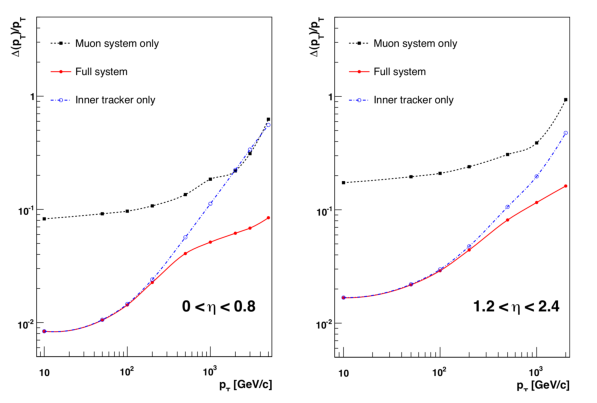
\includegraphics[scale= 1.2]{../Cap2/muon_res}
\caption{Trend resolution for the muon systems. On the left the barrel zone. On the right the endcap.}
\label{muon_res}
\end{figure}
\begin{figure}
\centering
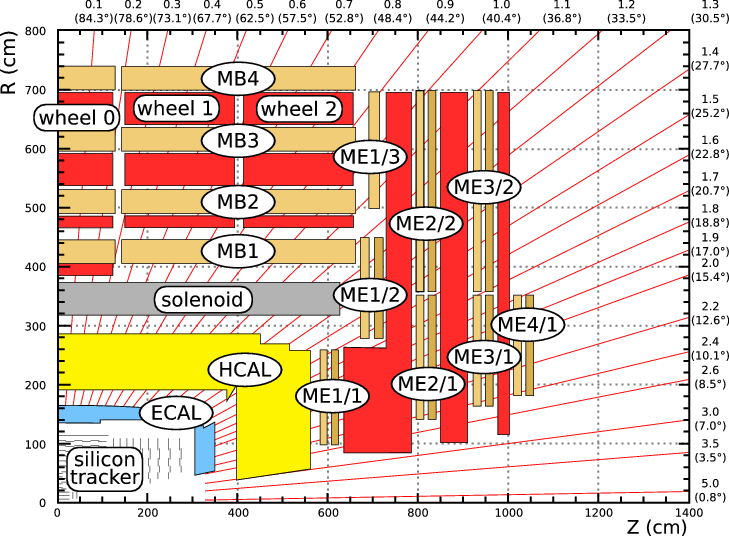
\includegraphics[scale= 0.4]{../Cap2/muon}
\caption{Schematic overview of the muon chambers.}
\label{muon_c}
\end{figure}


\subsection*{Trigger and Data Acquisition}
LHC can produce interactions at 40 MHz frequency, but only a small fraction of these
events can be written on disk. On one hand the speed at which data can be written
to mass storage is limited, on the other hand the vast majority of events produced is
not interesting, because it involves low transverse momentum interactions (minimum bias
events). Thus, a trigger system is needed to save interesting events at the highest possible
rate. The maximum rate of events written on disk is about 800 Hz. CMS has chosen a
two-level trigger system, consisting of a Level-1 Trigger (L1)  and a High Level Trigger
(HLT).
Level-1 trigger runs on dedicated processors, and accesses coarse level granularity information 
from calorimetry and muon system. A L1 Trigger decision has to be taken for
each bunch crossing within 3.2 $\mu$s. Its task is to reduce the data flow from 40 MHz to
about 100 kHz. The High Level Trigger is responsible for reducing the L1 output rate down to a maximum
rate of the order of 1 kHz. The HLT code runs on a farm of commercial processors and can access the full granularity information of all the subdetectors.

\section{Data recoiled and future plans}
The first proton beam circulated in the LHC on September 2008, after more than a decade of construction and installation.
An incident occurred between two magnets, causing the release of helium into the tunnel
and mechanical damage. After that, in March  2010 started the Run-I, a fruitful data taking era that lasted until
2012.  It was decided not to operate the LHC at its design parameters, and proton proton collisions
took place at a centre of mass energy of 7 TeV and 8 TeV. The amount of recoil data in this period is reported in Fig.~\ref{int_lumi_cumulative_pp_1}.

\begin{figure}
\centering
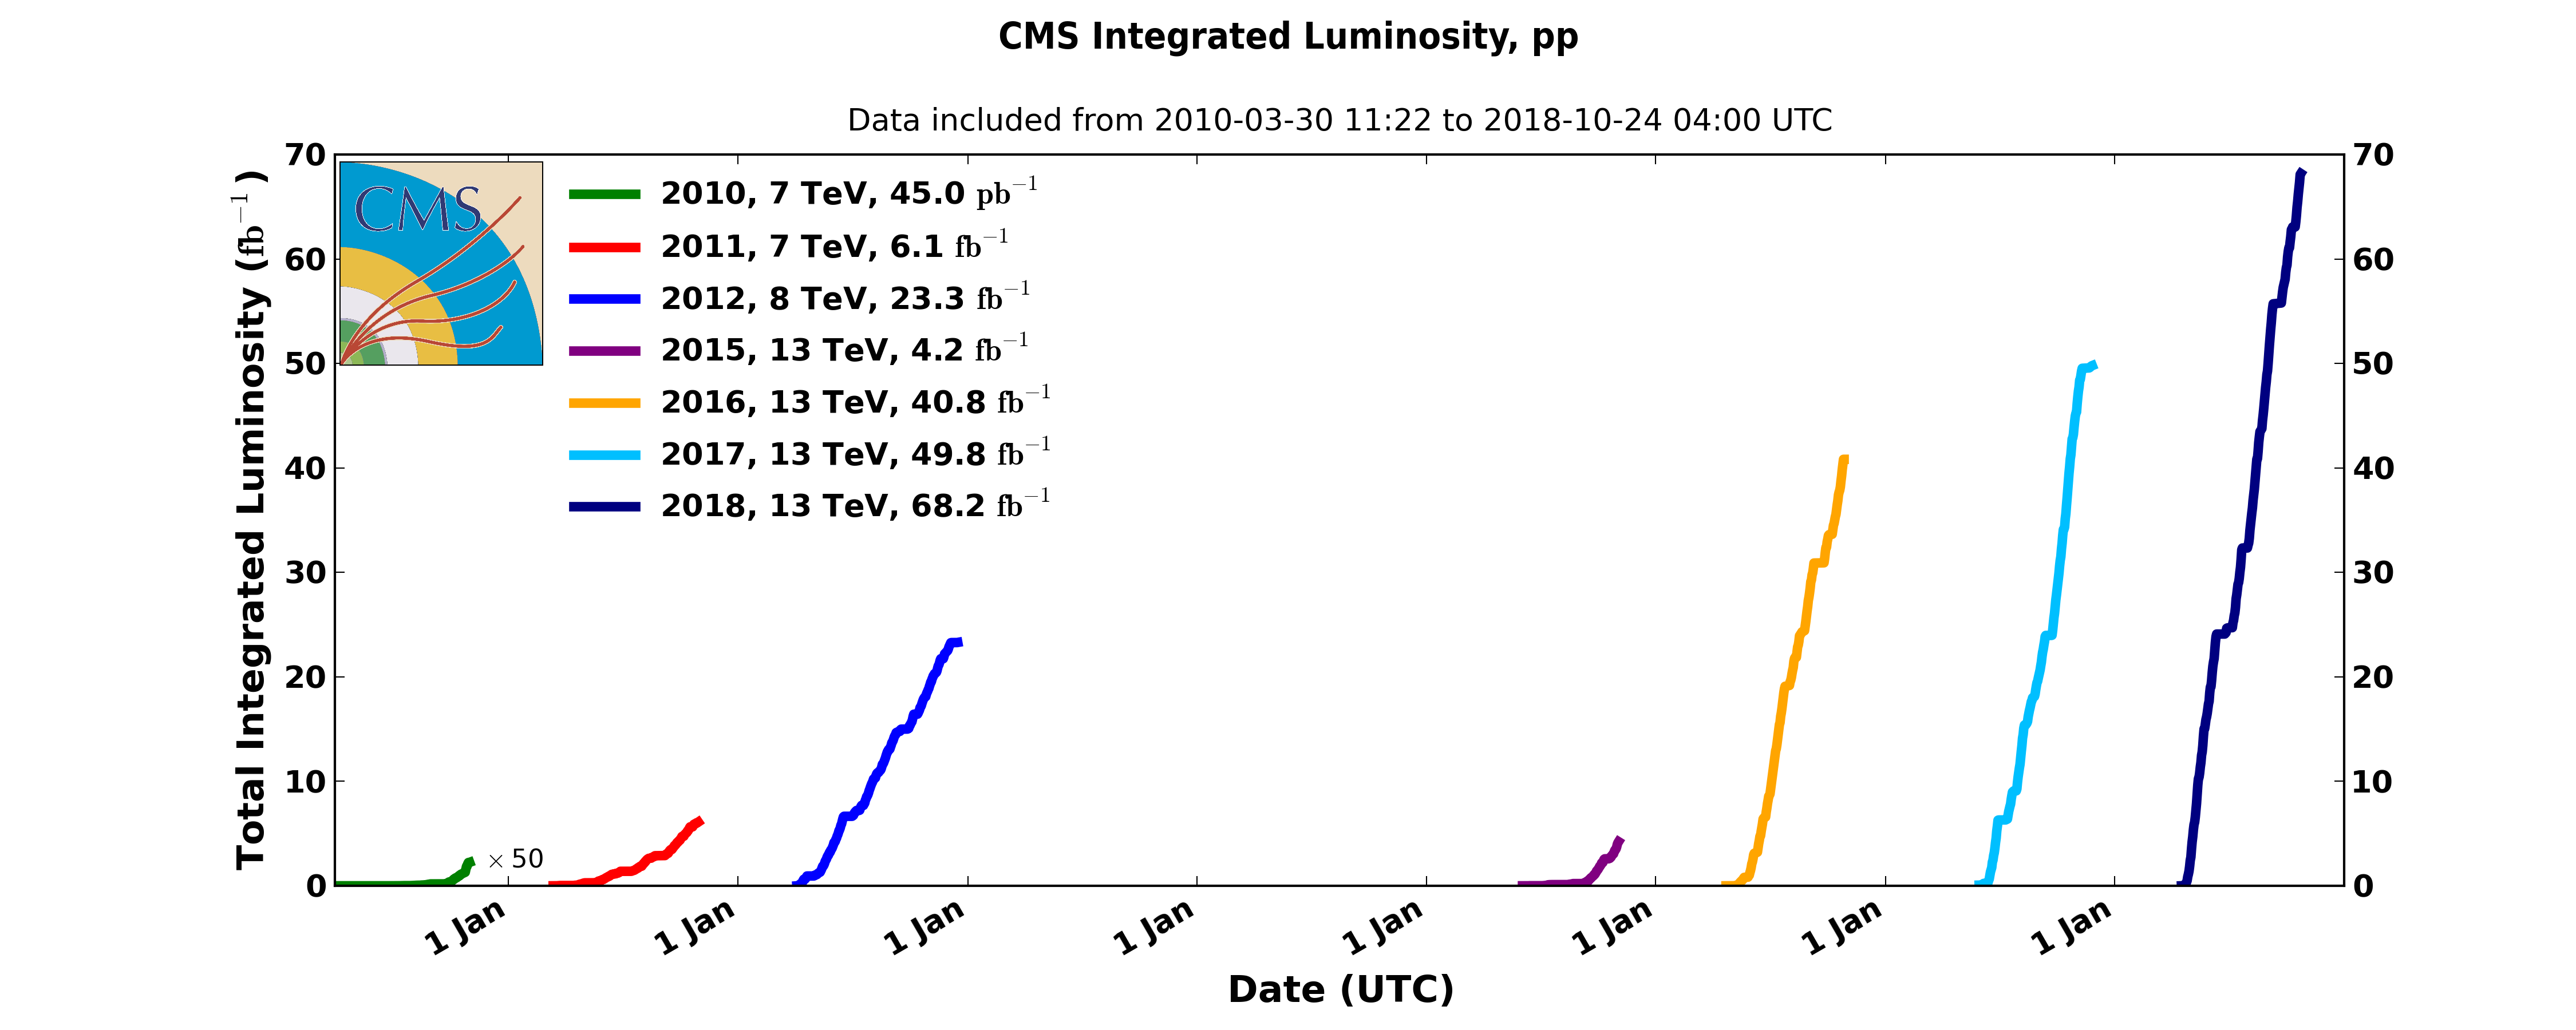
\includegraphics[scale= 0.4]{../Cap2/int_lumi_cumulative_pp_1}
\caption{Run-I ans Run-II integrated luminosity.}
\label{int_lumi_cumulative_pp_1}
\end{figure}

\begin{figure}
\centering
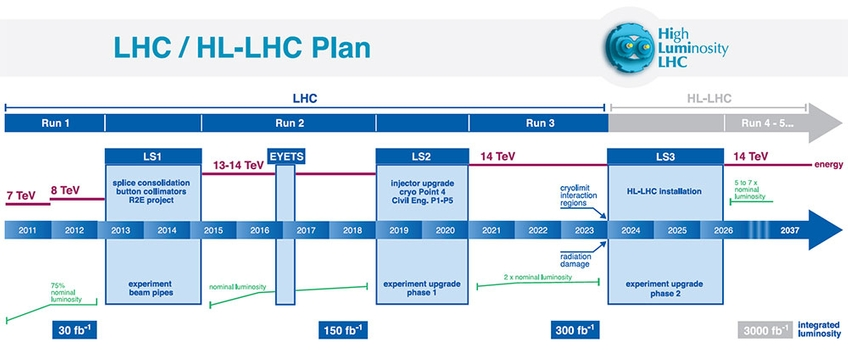
\includegraphics[scale= 0.5]{../Cap2/lhcplan}
\caption{Schedule of LHC and HL-LHC operations.}
\label{lhcplan}
\end{figure}




\begin{figure}
\centering
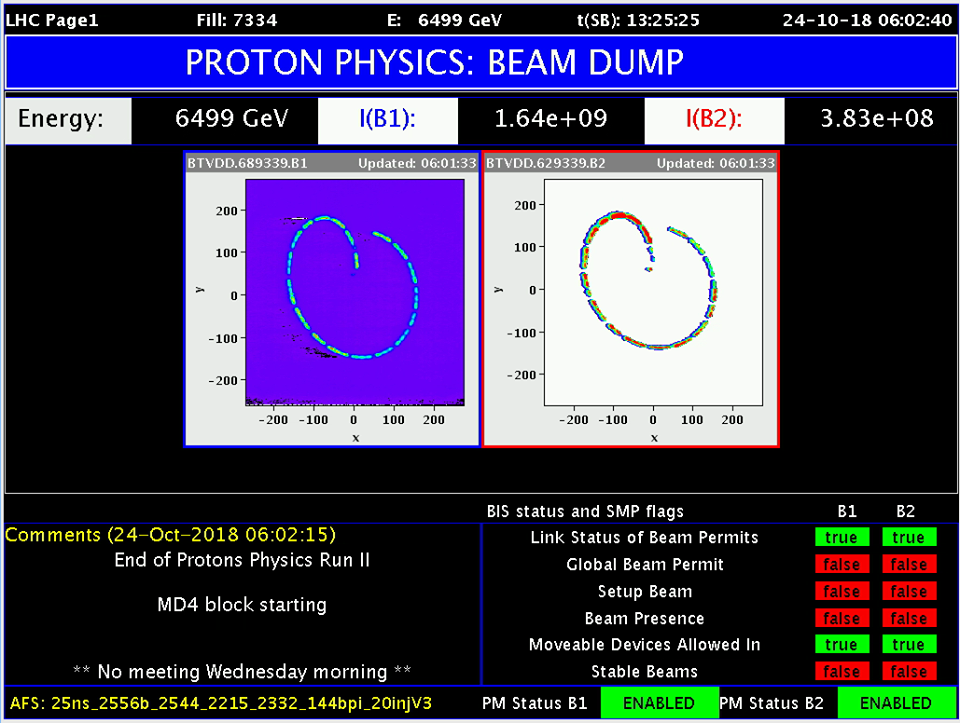
\includegraphics[scale= 0.2]{../Cap2/beam}
\caption{Last proton-proton beam dump at the end of Run-II.}
\label{int_lumi_cumulative_pp_1}
\end{figure}
} 
{\chapter{Monte Carlo Generators}
\label{cap3}


\textit{Hundreds of particles are produced In the collisions between high energy protons.
Given the complexity of the events, it is necessary to use Monte Carlo generators, i.e. programs that allow to simulate realistically the result of the collisions, assuming a certain model for the processes involved. In this chapter the various steps of Monte Carlo events simulation are described. During my work, contributing to the Monte Carlo production and validation of simulated eventshas been one of my main tasks.}

\section{General Overview}
The use of Monte Carlo generators is necessary because it is impossible to predict what happens event-by-event: in fact,  in quantum mechanics we can only calculate the probability of having a certain result.
The simulation of an event is carried out in successive steps \cite{Sjostrand:2006su, Buckley:2011ms}, as schematized in Fig.~\ref{qqqq}, thus subdividing the problem into several parts of lower complexity.


\begin{figure}
\centering
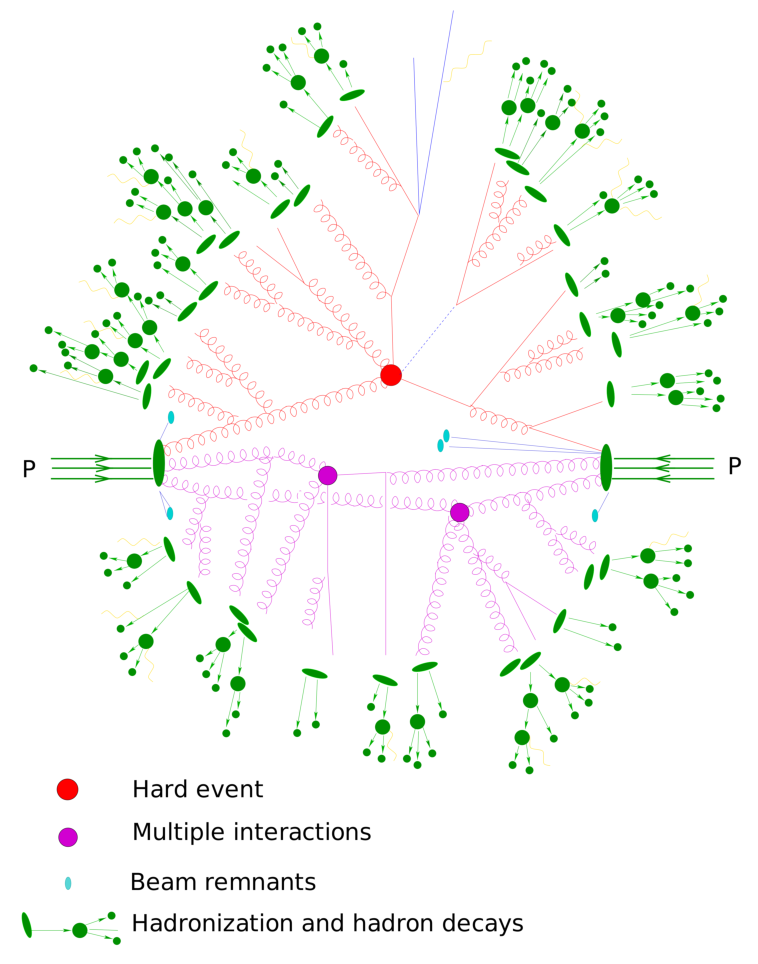
\includegraphics[scale= 1]{../Cap3/Fig_MC/generalMC}
\caption{Schematic representation of an event generated within an event generator. The partons coming from the protons indicative participate in both the hard process and multiple interactions. Subsequently there is the hadronization.}
\label{qqqq}
\end{figure}
The various steps are summarized here:
\begin{itemize}

\item Hard process: the incident protons are composed by  partons (quarks and gluons) and the hard process consists in a collision between two partons, coming from different hadrons. The  matrix element of the process is evaluated perturbatively and often only the lowest perturbative order, called leading order (LO), is calculated.
\item Parton shower: the incoming or outgoing partons participating in the hard process can emit gluons. In fact, in analogy with the electromagnetic interaction, a particle with an accelerated color charge can radiate for the bremsstrahlung.
The gluons in turn, can produce quark-antiquark pairs thus generating the parton showers.
The emission of additional partons takes place mainly in the collinear space respect to the initial parton and  progressively with less energies.
In the final state there will be a set of partons, called jet, located in the collinear with respect to the initial parton.
This probabilistic process can be simulated as a Markov process and is implemented in the parton shower algorithms we will discuss later.

\item Multiple interactions: in a single collision, it may happen to have more pairs of partons interacting. In this case it is said that there are multiple interactions in addition to the hard process.

\item Hadronization: in the evolution of the event the partons are generated with gradually lower relative momenta. 
For momentum values of 1 about GeV the confinement forces prevail. At these energy scales, the perturbation theory fails in the description, so we resort to non perturbative models which describe the formation of real hadrons. This hadronization process  preserves the jet structure which can therefore be observed experimentally.

\item Decaying of unstable particles: many of the particles produced in the primary process are unstable and they  decay unless they interact before with the detector.

\end{itemize}

In the  Monte Carlo simulation  all these steps are considered sequentially: the result of each step is the starting point of the next.
At the end, in a single event, there are hundreds of particles each of which has a dozen degrees of freedom (mass, flavor, impulse, average life, spin, vertex production, etc.), so there is a  high number of parameters that came into play and must be simulated for each event.
The final aim is to provide a realistic description of what happens in high-energy collisions, in order to compare the Monte Carlo model with the experimental data.
Schematically, the cross section of the final state is given by,
\begin{equation}
 \sigma_{final \: state}=\sigma_{hard \: process} \cdot \: \mathcal{P}_{tot, \:hard \: process \rightarrow final \:state} \: \mbox{,}\end{equation}
integrated over the total phase space and summed over all possible final states (e.g. the production of two or more jets). This is the measurable quantity associated with the hard process. \\




\section{Hard process}

In many processes of interest to LHC, high momenta come into play, to produce high mass particles or  energetic jet. The simulation of these events is the main goals of the Monte Carlo generators.
The cross section for a scattering $ ab \rightarrow n $ process is given \cite{Buckley:2011ms} by,
\begin{eqnarray}
 \sigma & = & \sum_{a,b}  \int_{0}^{1} \, dx_{a} dx_b \int f_{a}^{h_1} (x_a , \mu_F) f_{b}^{h_2} (x_b , \mu_F) \: d \hat{\sigma}_{ab \rightarrow n}(\mu_F , \mu_R)  \nonumber \\
& = & \sum_{a,b}  \int_{0}^{1} \, dx_{a} dx_b \int d \Phi_n  f_{a}^{h_1} (x_a , \mu_F) f_{b}^{h_2} (x_b , \mu_F) \nonumber \\
 & \times& \frac{1}{2\hat{s}} 
 | \mathcal{M}_{ab \rightarrow n} 
(\Phi_n , \mu_F , \mu_R)|^2  \: \mbox{,} \end{eqnarray}
where
\begin{itemize}
\item $f_{a}^{h} (x , \mu)$ are the parton density functions (PDF) that depend on the $x$ fraction of the parton $a$'s energy (Bjorken variable) respect to the 
hadron $h_i$ ($i=1,2$), and on the $\mu_F $ factorization scale, App~\ref{pdfa}.
\item $\hat {\sigma}_ {ab\rightarrow n} $ is the partonic cross section of the process $ ab \rightarrow n $.
The total differential cross section is given by the product of the corresponding square matrix element, $ | \mathcal {M}_{ab \rightarrow n} |^2 $, 
with  the incident particle flow $ 1 / (2 \hat{s}) = 1 / (2 x_a x_b s) $, where $ \sqrt{s} $ is the energy of the system's center of mass.
\item The matrix element $| \mathcal{M}_{ab \rightarrow n}  (\Phi_n , \mu_F , \mu_R) |^2 $  can be written as the sum on all Feynman diagrams,
\begin{equation}
\mathcal{M}_{ab \rightarrow n}= \sum_{i} \mathcal{F}_{ab \rightarrow n}^{(i)} \: \mbox{.} \end{equation}
\item $d\Phi_n$ it is the phase space differential for $ n $ particles in the final state.
\end{itemize}
The phase space will not be all physical space  but will contain cuts for two reasons: the first is that  the cuts will reflect the geometry and acceptance of the detector; the second because it is necessary put a cut on the transverse impulse of the particles produced in the process to avoid divergences in the calculation of the cross section \footnote {You can imagine having a singularity similar to that  in classical Coulomb scattering.}.
In general, the calculation of the matrix element would require the calculation of all the Feynamn diagrams which  grow in a factorial way (Fig.~\ref{fatt}) with the number of particles in the final state.
\begin{figure}[h]
\centering
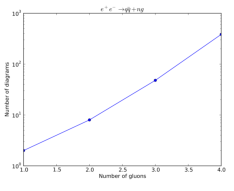
\includegraphics[scale= 2.5]{../Cap3/Fig_MC/fattoriale}
\caption{ Trends in the number of Feynman diagrams as the number $ n $ of gluons increases in the process $e^+ e^- \rightarrow q \bar{q} + ng$.}
\label{fatt}
\end{figure}
Usually the  Monte Carlo events generators can compute the matrix element at the leading order for the Standard Model $2 \rightarrow 1$,  $2 \rightarrow 2$  
and  $2 \rightarrow 3$ \cite{bib:madgraph} processes.  \\
However, if we stop at the first perturbative order, we would have only a rough description of the process: in fact, subsequent orders involve important corrections both to the shape of the distributions and to the total cross section. LO is useful for a first study but  it is important to evaluate next-to-leading-order (NLO) \footnote{For some particularly important processes, for example $ gg \rightarrow H $, the next-next-to-leading-order (NNLO) calculations are even available.}. \\
The cross section calculated at the NLO is composed of three parts: the LO part or Born, by the real and by the virtual part of the emission corrections (Fig. \ref{nlofig}),
\begin{equation}
 \label{xsecNLO}
 d\sigma^{NLO} =  d \tilde{\Phi}_n [\mathcal{B} (  \tilde{\Phi}_n  ) + \alpha_s \mathcal{V}(  \tilde{\Phi}_n  ) ] +  d \tilde{\Phi}_{n+1} \alpha_s \mathcal{R}(\tilde{\Phi}_{n+1}  ) \: \mbox{,}   \end{equation}
 where $\mathcal{B}$, $\mathcal{R}$ and $\mathcal{V}$  denote the Born, the real  and the virtual part respectively. The integral must be made on the $ n $ or $ n + 1 $ final state particles and on the Bjorken variables related to the incident partons.
Consider, in the Born approximation, the process  $ 2 \rightarrow 2 $. If you want to go to the next order, NLO, you have to keep the element with an additional parton in the final state, the $ 2 \rightarrow 3 $ process, and virtual correction with a loop in the $ 2 \rightarrow 2 $ process.
It should be noted that the cross-section for processes of the type $ 2 \rightarrow 3 $ is divergent when the energy of one of the partons tends to zero (soft divergence) or when two partons are collinear (collinear divergence).
\begin{figure}
\centering
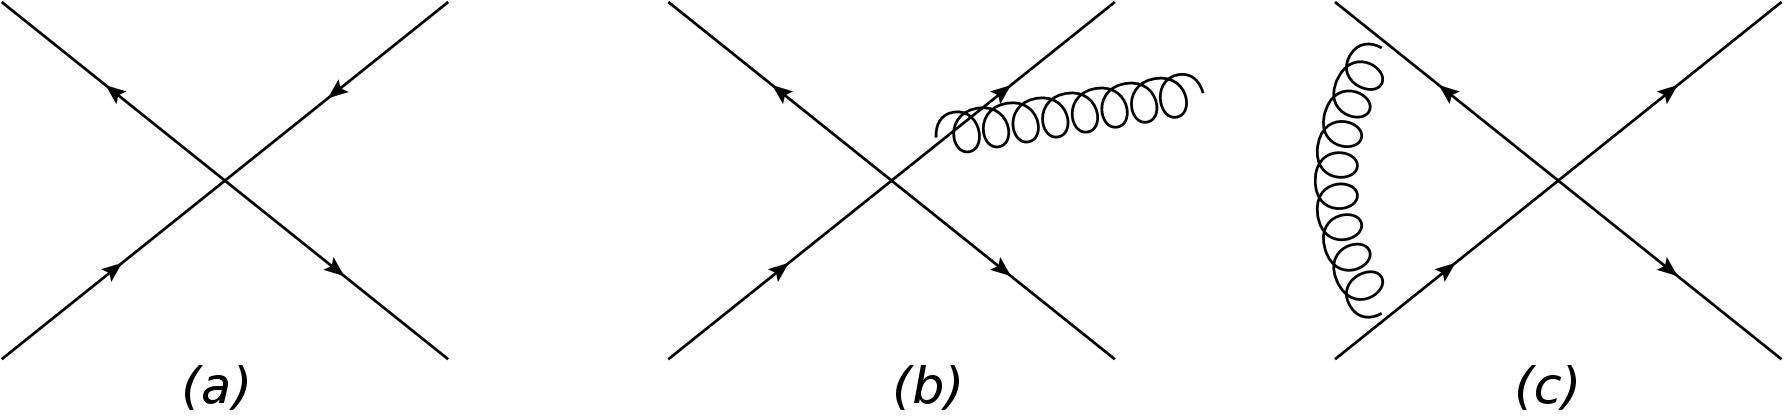
\includegraphics[scale=0.22]{../Cap3/Fig_MC/nlo2}
\caption{ Examples of Feynman diagrams (a)  Born, (b) real, (c) virtual. }
\label{nlofig}
\end{figure}
\section{Parton shower}
\label{ps}
In a collision between partons a charge of color is accelerated, so there will be bremsstrahlung emission. When studying a process of the type $ 2 \rightarrow n $, where $ n $ represents the number of partons in the final state, the LO matrix elements (called tree-level) will have divergences in the collinear  and 
soft case. In particular, the processes that suffer from this type of divergence are $ q \rightarrow qg $, $ \bar{q} \rightarrow \ bar{q} g $, $ g \rightarrow gg $: the first are similar processes to $ e \rightarrow e \gamma $ in QED, while the third is due to the fact that QCD is not an Abelian theory. The process $ g \rightarrow q \bar {q} $ does not have this type of divergence.
The divergences of the tree-level matrix element can be removed by introducing the virtual corrections into the calculation, but they will be in the next order; these calculations are therefore particularly complex and they are only possible for a limited number of processes. The parton shower \cite{Sjostrand: 2006su} algorithms offer an alternative and simple way to eliminate the collinear and soft divergences through:
\begin{itemize}
\item an iterative structure that combines the three states suffering from divergences in a single multi-partonic state,
\item the introduction of the form factor of Sudakov.
\end{itemize}
The incoming or outgoing partons, which are far (temporally) from hard process, are called on-shell. Indeed the module of their four-momenta   is equal to the mass at rest.
However, the closer one gets to the interaction,  the more  partons can be off-shell, i.e. the module of the their four-momenta does not correspond to the mass at rest due to the uncertainty principle ($ \Delta E \Delta t \sim \hbar $),. 
For this reason they are able to emit other partons and  the energy of emitted partons is higher if they are closer to the scattering.
If the emission occurs before the scattering, it is called initial state radiation (ISR), while after the interaction it is called final state radiation (FSR). \\
Each parton  is characterized by a  ``virtuality scale'' $Q^2$ that corresponds roughly to a shower temporal scale.
It is important to stress that different definitions are available for $Q^2$; however regardless of the chosen convention, the $ Q^2 $ scale increases as it approaches the hard process,  in the ISR, and decreases away, in the FSR. If we take the FSR,  the evolution starts at a $ Q^2_ {max} $ scale that is related to the hard process and it ends when a limit scale is reached, $ Q_0 $, which will be on the order of 1 GeV .\\
The most common choice used is to set  $Q^2=p^2=E^2- |\vec{p}\,|^2$. With this convention in a process of type  $a \rightarrow bc$, in FSR case, $Q^2 >0$, 
$Q$ is time-like, decreases until the limit scale $ Q_0 $ is reached.
The ISR case is complicated. In this case, if $c$ is an emitted parton that will not participated in the hard interaction, $a$ and $b$ are off-shell. The are space-like and in order to guaranteed the increase order of $Q^2$,  i.e. $ Q_b^2> Q_a^2 $, it is better to define  $ Q_i^2 = -m_i^2 $. In contrast $c$ is time-like 
Therefore its shower will evolve like that of the FSR.

\subsection*{Final State Radiation}
In the parton shower approach, the final state radiation  is modeled through a series of divisional processes of the type $ a \rightarrow bc $.   
This is evident from the process $q \bar{q}g$, Fig. \ref{nlofig} (b), where the first order matrix element  corrections  correspond to the emission of a gluon. 
The evolution of the shower is described by two parameters: the fraction of energy carried by one of the two outgoing partons, $ z = E_b / E_a $, and the order variable $ t $. As we said, a possible choice for $ t $ is the  virtuality $ Q_a^2 $ of the incoming parton.
In the  collinear limit the probability of division $d \mathcal{P}_{a \rightarrow bc}$, in  $z$ and $t=\ln(Q^2/\Lambda^2)$ is:
\begin{equation}
 d \mathcal{P}_{a \rightarrow bc}=  \frac{\alpha_{abc}}{2 \pi}\: {P}_{a \rightarrow bc} \:dt dz  \: \mbox{,} \label{prob}  \end{equation}
where $dt=\frac{d Q^2}{Q^2}$, $\alpha_{abc}$ it is the coupling constant that regulates the division process and  ${P}_{a \rightarrow bc}$ is the kernel splitting; these are universal functions and are valid in the collinear limit:
\begin{eqnarray}
P_{q \rightarrow qg    }&=& \frac{4}{3} \frac{1+z^2}{1-z} \mbox{,} \nonumber \\ 
 P_{g \rightarrow gg }&=& 3 \frac{(1-z(1-z))^2}{z(1-z)}    \mbox{,} \\ 
P_{g \rightarrow q\bar{q} }&=& \frac{n_f}{2} (z^2+ (1-z)^2)   \mbox{,} \nonumber \end{eqnarray}
where $n_f$ is the quarks flavour number.
However the probability  evaluated is larger than the unity. Indeed it suffers from the same divergences of the matrix element at the LO. 
The expression \ref{prob} is evaluated in the collinear approximation. 
In particular, there are two types of divergences: collinear, due to the dependency of type $ 1 / Q^2 $, and soft which corresponds to the limit $ z = 1 $. \\
To solve this problem, in the parton shower approach, the probability of dividing $ t $ and $ t + dt $ is evaluated; this is obtained with the integration of Eq \ref{prob} over  $z$ in the intervals  $[z_{min}(t), \: z_{max}(t)]$:
\begin{equation}
 d \mathcal{P}_{a}= \left( \sum_{bc} \int_{z_{min}(t^{'})}^{{z_{max}(t^{'})}}  \frac{\alpha_{abc}}{2 \pi}\: {P}_{a \rightarrow bc} \: dz \right) dt  \: \mbox{.}   \end{equation}
As in other physical situations \footnote{For example radioactive decay.} the probability of something happening at $ t $ is given by the probability that this happens between $ t $ and $ t + dt $, multiplied by the probability that this has not already occurred between the initial instant $ t_0 $ and $ t $.
In this case then the  division probability  at $ t $ is:
\begin{equation}
 d \mathcal{P}_{a}^{\mbox{\footnotesize{FSR}}}(t)=   d \mathcal{P}_{a} \cdot \mbox{exp} \left(   -\sum_{bc} \int_{t_0}^t dt^{'}  \int_{z_{min}(t^{'})}^{{z_{max}(t^{'})}} \frac{\alpha_{abc}}{2 \pi} P_{a \rightarrow bc}(z) dz \right) \mbox{,}\end{equation}
where $t_{0}$ is the shower starting scale. 
The exponential term is called Sudakov factor and it represents the probability of non-division. 
If you want to interpret it in terms of Feynman diagrams, this represents the virtual corrections of LO matrix element. \\
This total process can be combined to have more emissions at different steps: this will result in a partons  shower which will be ordered in decreasing $ Q $. 
Finally,  the description given by parton shower is correct if you have collinear jet and it fail in configurations where there are well separated partons.   

\subsection*{Initial State Radiation}
The initial state radiation evolution is much more complicated than the final state. 
Indeed the quark and the gluons are   emitted  and absorbed continuously, inside the incoming proton. The initial stare radiation is already present during the hard scattering.
The ISR simulation could start from the on-shell parton before the interaction and after  could evolve to higher and higher $ Q ^ 2 $ scales until the hard process.
However, this approach is very inefficient because the  interesting  process  is particularly rare and  it has the same probability to happen as in nature. 
In the event generators a different approach is  used: first the hard process is produced and then  we try to rebuild back what may have happened. 
This procedure is called backward evolution, Fig. \ref{isr}.
It is necessary to evaluate the  probability for the process of type $ a \rightarrow bc $,  that a parton $ b $ has  been produced by the parton $ a $.
For this reason the  partonic density function is introduced.  This evolves according to the DGLAP \cite{Altarelli: 1977zs} equation,
\begin{figure}
\centering
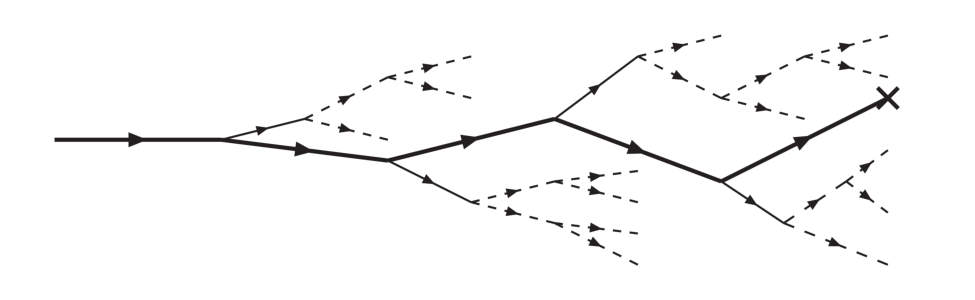
\includegraphics[scale= 0.8]{../Cap3/Fig_MC/isr}
\caption{ Evolution of the initial state. The bold line corresponds to the part that will undergo the hard process (represented by a cross). Thin lines represent the partons that can not recombine, while the dashed lines are fluctuations that may or may not recombine.  }
\label{isr}
\end{figure}

\begin{equation}
  \frac{d f_b(x, \:t)}{dt}= \sum_{ac} \int_x ^1 \frac{d x^{'}}{x^{'}} \: f_a(x^{'},t) \:\frac{\alpha_{abc}}{2\pi} \:P_{a \rightarrow bc} \:(\frac{x}{x^{'}}) \mbox{,}\end{equation}
where $f_{a,b}(x, \:t)$ are the parton PDFs  $a$, $b$, that which have $ x $ fraction of the incident and scale proton momenta $t=\mbox{ln}(Q^2/ \Lambda^2) $, instead $P_{a \rightarrow bc}$ is the kernel splitting function.\\
In the backward evolution the probability that the parton $ b $ has been generated from $ a $ in the interval between $ t $ and $ t-dt $ is given by:
\begin{equation}
d\mathcal{P}_{b}(t)=\frac{d f_b(x, \:t) }{ f_b(x, \:t)}= |dt| \sum_{ac}  \int  \frac{d x^{'}}{x^{'}} \frac{d f_a(x^{'}, \:t) }{ f_b(x, \:t)} \frac{\alpha_{abc}}{2\pi}          \:P_{a \rightarrow bc} \:(\frac{x}{x^{'}})      \mbox{,}\end{equation}
while the probability of non-division between the scale $t_{max}$ and $t<t_{max}$ is:
\begin{equation}
S_b (x,t,t_{max})=   \mbox{exp} \left( - \int_t ^{t_{max}} dt^{'} \sum_{ac}  \int  \frac{d x^{'}}{x^{'}} \frac{d f_a(x^{'}, \:t^{'}) }{ f_b(x, \:t^{'})} \frac{\alpha_{abc}}{2\pi}          \:P_{a \rightarrow bc} \:(\frac{x}{x^{'}}) \right)     \mbox{,}\end{equation} 
Finally the probability of combining $ b $ in $ a $ in the range between $ t $ and $ (t-dt) $ from is:
\begin{eqnarray}
d \mathcal{P}_{b}^{\mbox{\footnotesize{ISR}}}(t) &=& - \frac{d S_b (x,t,t_{max})}{dt} dt \nonumber \\
&=&  \sum_{ac}  \int  \frac{d x^{'}}{x^{'}} \frac{d f_a(x^{'}, \:t) }{ f_b(x, \:t)} \frac{\alpha_{abc}}{2\pi}          \:P_{a \rightarrow bc} \:(\frac{x}{x^{'}})  \cdot S_b (x,t,t_{max}) dt \end{eqnarray}
In this case the Sudakov  form factor is different respect to FSR as it contains the PDFs.
This means that the parton shower results do not depend only on the algorithm but also on the PDFs used.

\subsection*{Resummation} When calculating an observable predicted by QCD in a perturbative way, the expansion in powers of $ \alpha_S $ contains terms of the type $ \alpha_S^n L^k $ ($ k < 2n $), where $ L = \ln (q_{cut} / s) $, being $ q_{cut} $ the cut on resolvable emission. 
When we consider small values of  $q_{cut}$ the logarithm of the perturbative expansion becomes large and the  perturbative series diverges.
The main  perturbative order of the expansion is $n$  only if the successive terms of the series are negligible, however this is not guaranteed if there are high value of L. 
It is therefore necessary to consider the terms that have a high value of the logarithm. The study of these terms is called resummation and is done by putting the terms together in the perturbation series according to their degree of divergence:
$ \alpha_S ^ n L ^ {2n} $ are the leading log (LL) terms, $ \alpha_S ^ n L ^ {2n-1} $ are the next-to-leading log (NLL) terms, and so on. 
At the end  all $ \alpha_S $ orders terms are added. For many processes calculations are available at the NLL.
The parton shower approximate the effects of resuming at the NNLL. 

\subsection*{Merging among ME and PS}
The two different approaches for the  matrix element calculation  and for the parton shower have advantages and disadvantages. Regarding the ME we have:
\begin{itemize}
\item the LO matrix element calculations  can be performed exactly in the cases where there are many jet (of the order of six) in the final state,
\item a good description of separate partons is performed,
\item the perturbative calculations are correct,
\item however, the cross section diverges in the collinear and soft case, so an exhaustive description of the internal structure of jet is not possible.
\end{itemize}
On the other hand the PS:
\begin{itemize}
\item it is a universal approach that produces a realistic configuration of the partons,
\item the divergences, in the collinear limit, are treated with the introduction of the form factor of Sudakov. So we have an appropriate description of the jet evolution
\item however, the method fails when describing separate partons, since the collinear approximation in this case can not be valid.
\end{itemize}
Clearly the two methods are complementary and their merging is desirable. 
There are different approaches that combine ME with PS. The main difficulty is to cover the total phase space without overlaps or holes: we want to describe a process in which there are $ n $ well separated partons in the final state, using the LO matrix element  but  also including the  large logarithms resummation (LL, NLL) which is typical of the PS. A schematic description of the combination for four jet is given in Fig. \ref{merge}.
On the horizontal axis are the $ \alpha_S $ coupling orders, while on the vertical axis  the logarithm.
The PS includes the LL ($ m = 2n $) and the NLL ($ m = 2n-1 $) green circles (e.g. in the case of $ n = 2 $, $ m = $ 4, 3 the two circles  in green  marked as ``4'').
The circles that describe the event with four jet, when combining  the ME and  PS, are  green, the blue  and  three red  circles marked with the `` 4 ''.
The difficulty arises because the ME describes exactly all the circles marked with the `` 4 '': so if we simply sum up the two approaches 
we would  double counts these green circles.
\begin{figure}
\centering
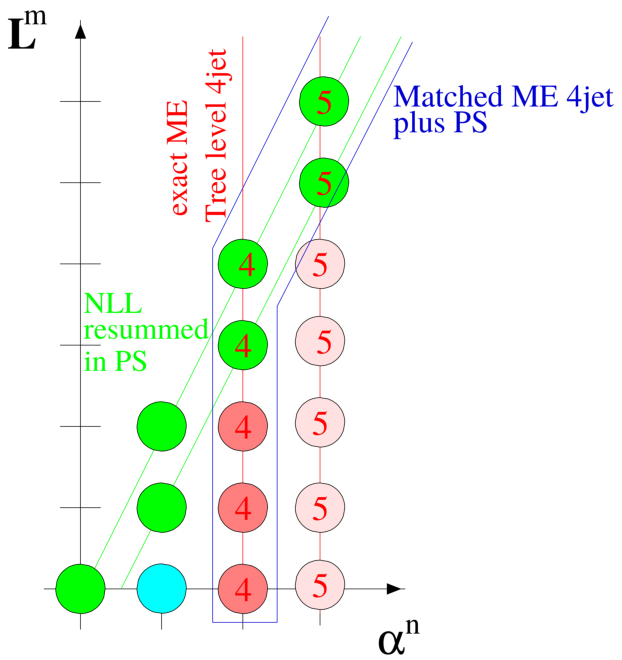
\includegraphics[scale= 0.7]{../Cap3/Fig_MC/merge}
\caption{ Merging among ME and PS.}
\label{merge}
\end{figure}
The most used approaches to merge the  ME and PS are:
\begin{itemize}
\item  parton shower reweight: the basic idea is to start from the process to the lowest order and then re-evaluate the output of the PS as if it had been produced by the ME. This approach does not change the cross section, which remains at the lowest order, but improves the population of the phase space \cite{ripesamento, ripesamento2}.
\item  CKKW prescription: the phase space is divided into two zones using $ k _ {\ perp} $ which is a measure of the cut $ Q_0 ^ 2 $: the region in which the jet is produced is filled with the ME, that of evolution with the PS \cite{ckkw, ckkw2}. 
\item The MLM prescription, which is also very widespread, is based on the same principle, but is implemented in a different way.
\end{itemize}


\section{Multiple Interaction}
Incident protons participating in the interaction are composed by  large number of partons (quark and gluons) that can interact independently with each other in addition to the hard process.
The total cross section for the QCD process $ 2 \rightarrow2 $ is dominated by the $t$-channel, so the cross section diverges as $ d p _ {\ perp} ^ 2 / p _ {\ perp} ^ 4 $ for $ p _ {\perp} \rightarrow 0 $ \cite{Sjostrand: 2006su}.
So when simulating a real event, in addition to the hard event, characterized by having large transverse transverse momentum, we must also take into account the additional collisions at small $ p _{\perp} $. If these occur independently then a Poisson distribution is expected, $ P_n = \langle n \rangle ^ n \mbox {exp} (- \langle n \rangle) / n! $. However, conservation of energy and momenta means that interactions are not effectively independent, thus suppressing the possibility, for $ p_{\ perp} \rightarrow 0 $, of having a high number of interactions.
It should also be noted that in order to eliminate the divergence it is necessary to introduce a cut-off value of the transverse pulse, below which no collisions are generated.



\section{Hadronization }
In this context, the process of hadronization is a particular model, used in event generators, which describes the transition from the final partonic state to the final hadron state, which is an  experimental observable. It is important to underline that this transition is treated in a phenomenological way and not by a rigorous approach. The two most important classes for tuning are the string model and the cluster model. The difference is that the former transforms the partonic systems directly into hadrons, while the second takes an intermediate step where it groups the objects to a scale of $ \sim 1 $ GeV.

\subsection*{String Model}
The Lund model is the most complete string model: we know from QCD that there is a linear confinement force between the partons that increases with distance. Consider, as an example, the final state in which there are two quark, $ q \bar{q} $. As the partons move away the color flow tube is stretched between $ q $ and $ \bar{q} $, Fig.~\ref{tubo} (a). The transverse dimensions of the tube are the typical dimension for the hadrons, therefore  about 1 fm.
If the tube is assumed to be uniform, the potential increases linearly, $ V (r) = \kappa r $, with $ \kappa \approx $ 1 GeV/fm, string constant.
\begin{figure}
\centering
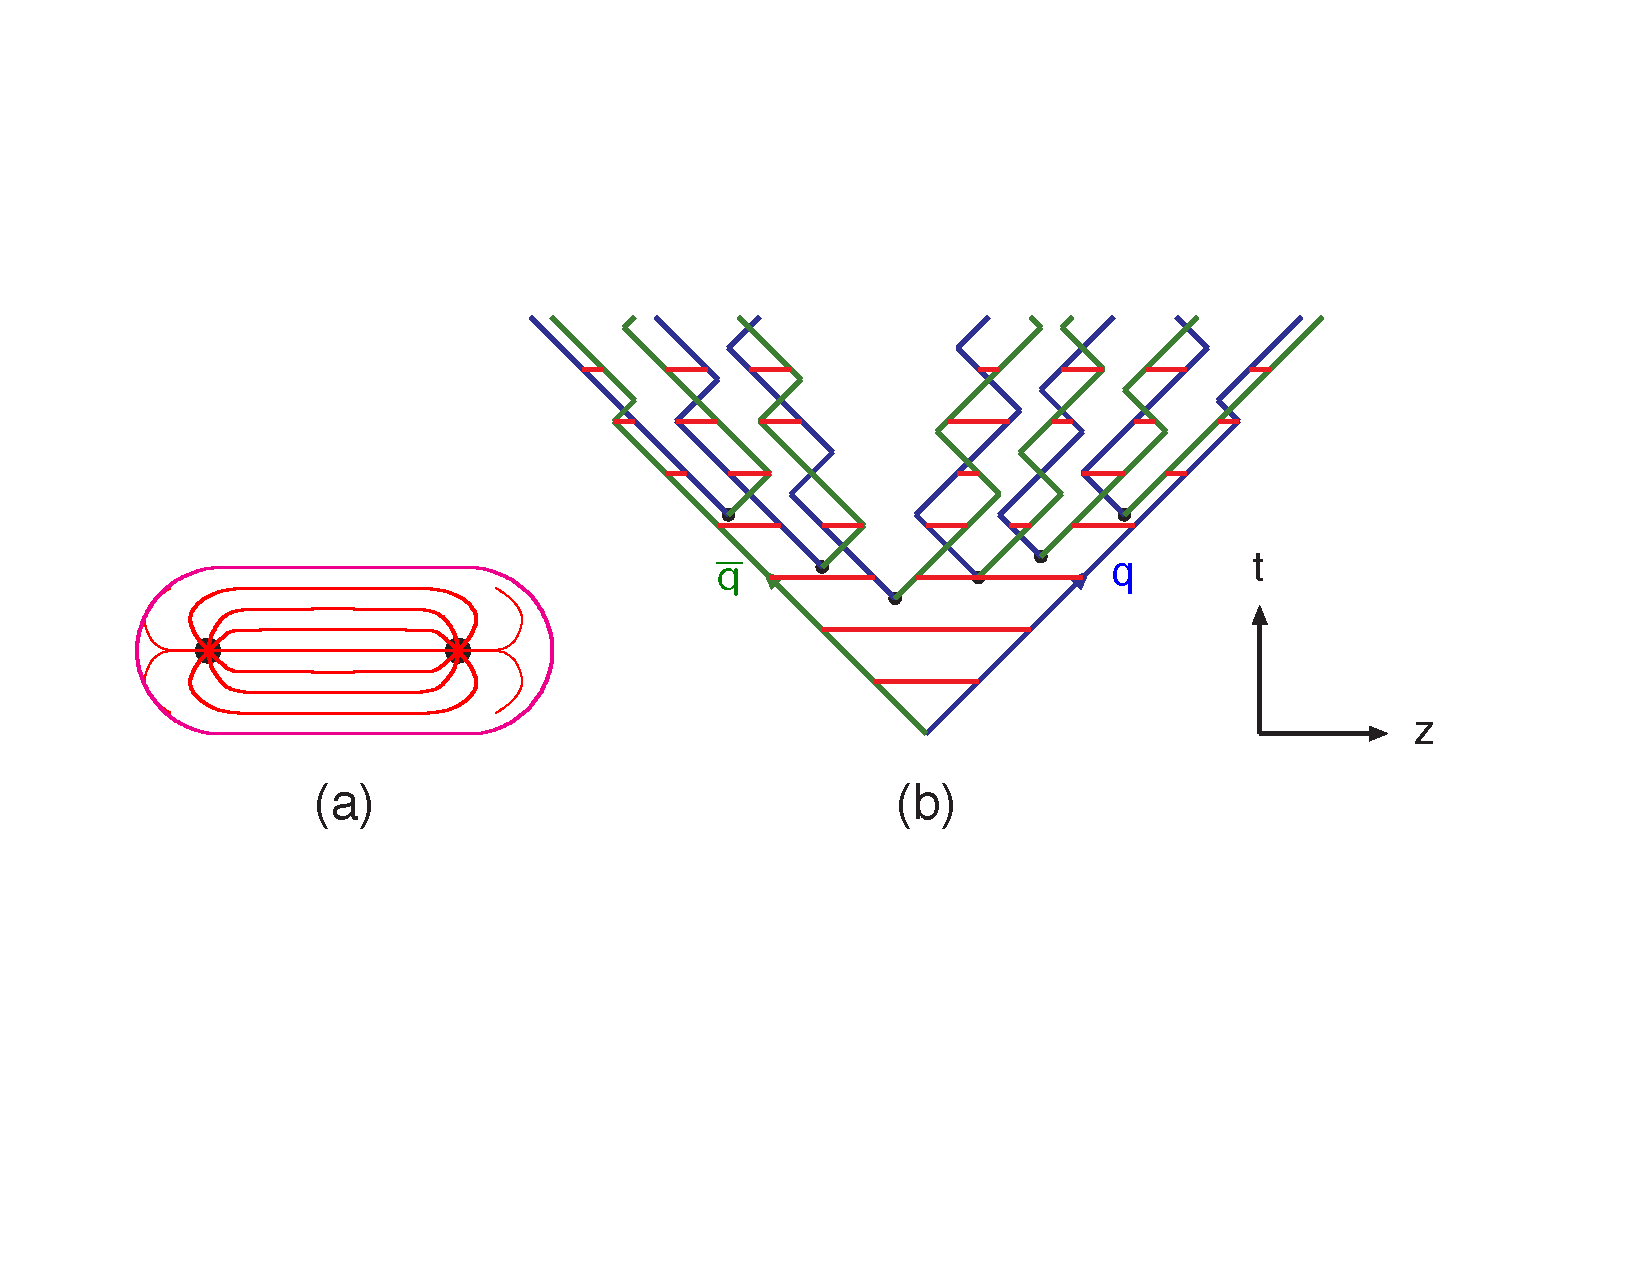
\includegraphics[scale= 0.5]{../Cap3/Fig_MC/stringone}
\caption{(a) The flow tube between a quark and an antiquark moving away. (b) Motion and breaking of a system string.}
\label{tubo}
\end{figure}
At short distances it would be necessary to introduce an additional Coulomb term, $ \sim \frac{\alpha_s}{r} $, however in the Lund model this term is  negligible.
As the quark and antiquark move away from the interaction vertex, the potential energy accumulated in the string increases until it breaks, giving rise to a pair $ q'  \bar{q}' $. So the system is divided into two new color singles $ q \bar{q} '$ and $ q' \bar{q} $. These two systems will move away  repeating the process below. The evolution of the system in space-time is represented in Fig.~\ref{tubo} (b).
At the end of the process  a serious of  $ q_i \bar{q_i} $ pairs are presented, each of which will form a hadron.
For now, only the case $ q \bar{q} $ has been considered. However, if more partons come from the interaction, the string model becomes more complicated. For an event in which there is an additional gluon, $ q \bar{q} g $, the string is stretched between $ q $ and $ g $ and between $ g $ and $ \bar{q} $, Fig. \ref{tubo3}.


\begin{figure}
\centering%
{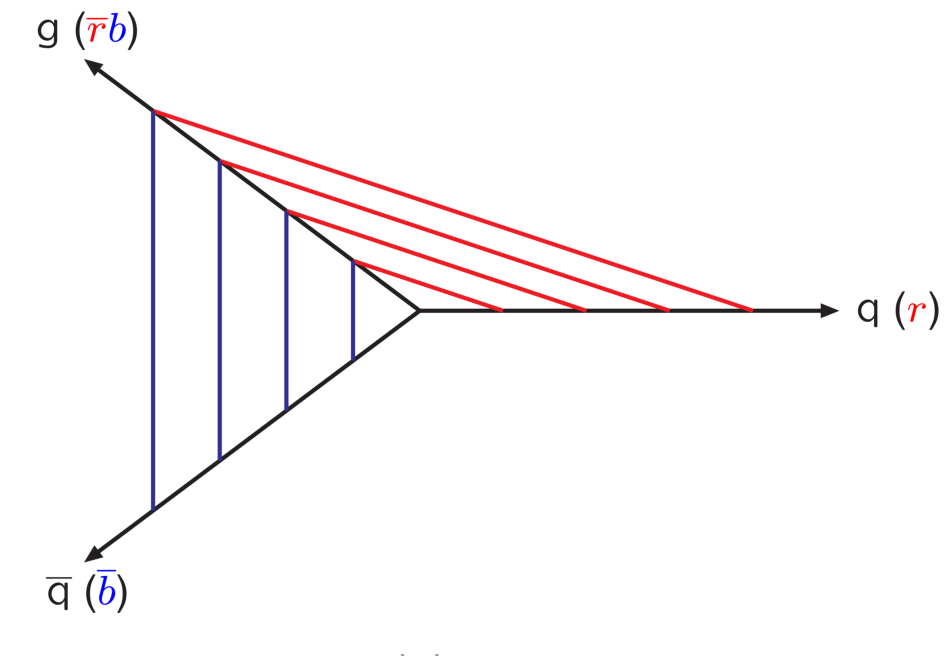
\includegraphics[scale= 0.5]{../Cap3/Fig_MC/stringtwo22}}
\caption{Motion of the string in the case $q \bar{q}g$.}
\label{tubo3}
\end{figure}

\begin{figure}
\centering%
\subfigure[]%
{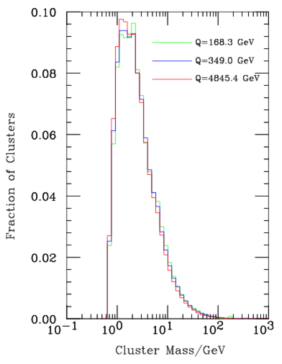
\includegraphics[scale= 1.5]{../Cap3/Fig_MC/split2}}
\subfigure[]%
{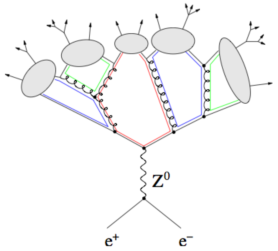
\includegraphics[scale= 1.4]{../Cap3/Fig_MC/split}}
\caption{(a)  Invariant mass distribution for singlets. (b) Parton shower structure in the cluster model.}
\label{tubo2}
\end{figure}


\subsection*{Cluster Model}  This  hadronization model  is based on the pre-confining property of the parton shower: 
the distribution of the invariant mass of a single pair of opposite-colored partons is the same at any $ Q^2 $ scale. 
The distribution increases rapidly at low value , Fig.~\ref{tubo2} (a). \\
In the model, the gluons from parton shower are represented by pairs of color-anticolor lines connected to the vertex. Each color line, near the cutoff, is connected to another colorless line present at the same scale. At this point the contiguous color/anticolor lines are interpreted, in the non-perturbative limit, as quark-antiquark pairs which give rise to mesons, which are observable objects in the final state.
This mechanism is represented in Fig.~\ref{tubo2} (b).

\section{Hadronic Decays and  Electromagnetic   Radiation.}
In the hadronization step, unstable hadrons which decay into other particles can be produced. So the final state  is the result of the convolution between the  hadronization  and the decay. The information necessary for the decay of unstable particles  is generally taken from the  ``Particle Data Book'' (PDG)~\cite{bib:pdg} which provides the properties (e.g. average life) of a large number of particles.
In general, in an event generator, it is necessary to choose which hadrons to include in the simulation and then select the possible decay channels. In addition to hadronic decays, it is also necessary to simulate the emission of electromagnetic radiation. The most common approach adopted is to use algorithms similar to those used to simulate the emission of QCD in parton shower.

\section{Jets} 
\label{rico_jet}
At the end of this process, after the hadronization and the decaying of  unstable particles it is still possible to estimate the four-momenta of the partons generated in the hard process as the direction and energy  of the jets  that are reconstructed  from the final state particles ~\cite{bib:run2jet}.
The jets are reconstructed by an algorithm that calculates the distance, $ d_ {ij} $, between two objects (particles or pseudo-jet ) defined as,
\begin{equation}
d_{ij}=\mbox{min}( k_{ti}^{2p}, k_{tj}^{2p})  \frac{\Delta_{ij}^2}{R^2} \mbox{,}\end{equation}
where $\Delta_{ij}^2=(y_i - y_j)^2+ (\phi_i - \phi_j)^2$ and $k_{ti}$, $y_i$ and $\phi_i$ are  the transverse momentum, the rapidity  e the azimutal angle of $i$ respectively. The constant $R$ is the radial parameter. The distance between  $ i $ and the beam  is also introduced , $d_{iB}=k_{ti}^{2p}$. \\
The algorithms proceed by calculating the minor distance $ d_{ij} $ between all the pairs of particles $ i $, $ j $. 
The four-momenta of the two particles with the smaller distance are added. The $ d_{iB} $ is evaluated for every $ i $ and if it is less than the distance $ d_{ij} $ with all other particles $ j $, $ i $,  than is is considered a jet and it is removed from list of objects present in the event.
Finally the distances are recalculated and this whole procedure is repeated until there are no more objects to be added.
For a value of $ p = -1 $ the algorithm is called anti-$k_t $ \cite{Cacciari:2008gp}. This is what has been used in this work, Sec.~\ref{jetr}.


\section{Main Monte Carlo generators }
For a proton-proton collision at the LHC, different Monte Carlo generators are available. Each of these has different methods for combining the ME with the PS.
A short introduction of  the main generators is given below. 
 
 
\subsection*{Madgraph\_aM{\footnotesize C@NLO}}
The \aMC \cite{bib:madgraph} approach is very ambitious, in fact the purpose of this generator is to calculate the cross section at the NLO including automatically both real and virtual contributions in the calculation. The  hard process is produced by the ME  while the soft emissions are added by the PS.
The first step is to compute the ME NLO corrections for a process involving $n$ partons. 
It results from  $n+1$ partons due to the real corrections and from $n$ partons due to the virtual corrections. 
As next step, it is evaluated  how the parton shower populates the phase space for $ n + 1 $ parton, excluding the Sudakov form factor. 
To get the state with $n+1$ partons, \aMC subtracts the PS  from the ME . 
The PS, without the Sudakov,  and the ME are in agreement in the soft and collinear limits, i.e. the singularities are deleted thus obtaining a finite value for the cross section for $ n $ and $ n + 1 $ partons. 
A technical problem arises in the collinear limit. Here, there is no certainty that the ME overhangs the PS everywhere. 
This problem is solved by introducing a fraction of negative-weight events, Fig.~\ref{weight}. 
Finally, the parton shower is applied, which includes the Sudakov factor and thus allows a finite and correct result to be obtained at the NLL. 
 \begin{figure}
\centering
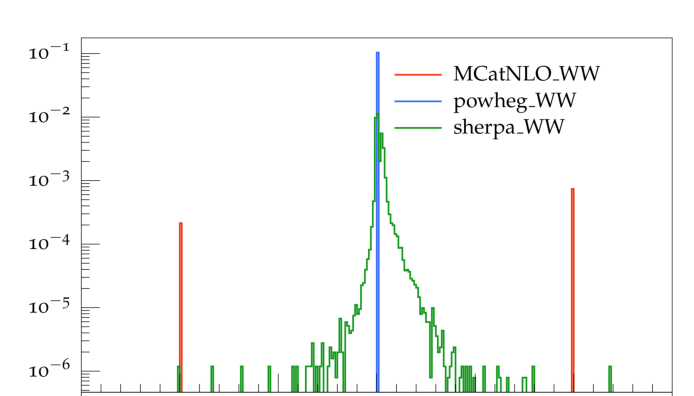
\includegraphics[scale= 0.7]{../Cap3/Fig_MC/weight}
\caption{Weight distribution, for different Monte Carlo generators, with cross section normalization of 1 fb$^{-1}$.}
\label{weight}
\end{figure}
 
\subsection*{P{\footnotesize OWHEG}} The idea behind P{\footnotesize OWHEG} \cite{Oleari:2010nx} is to generate the hardest radiation first, and then pass the event to the parton shower generator. In parton shower generators, the production, ordered in a transverse pulse, of the harshest radiation is always the first; so P{\footnotesize OWHEG} simply replaces this with the NLO emission.
In P{\footnotesize OWHEG} events are produced with a positive and constant weight (Fig.~\ref{weight}).
 
 
\subsection*{P{\footnotesize YTHIA}8 } P{\footnotesize YTHIA 8} \cite{bib:pythia} is a generator that can calculate the ME for processes with two particles or partons in the final state, but above all it generates the parton shower and the subsequent synchronization. The parton shower is ordered in a transverse impulse, $ p_T $, and the first issue is corrected with reweight method. For hadronization is used the Lund model.
 
 
\subsection*{S{\footnotesize HERPA}}  S{\footnotesize HERPA}  \cite{bib:sherpa} is a Monte Carlo generator that like PYTHIA8 provides a complete description of hadronic collisions, from the calculation of the matrix element, up to the stable particles. The parton shower includes both QCD and QED emissions, i.e. photons. It can calculate the ME for the main processes (eg $ gg \rightarrow H $) at the NLO and combine the ME with the PS. The code is written completely in C $ ++ $ language.




\section{Monte Carlo samples in High Mass Analysis}
\label{MSsample}
Several  Monte Carlo  generators were used in the searching of a high mass particle to simulated the signal and the backgrounds. 
All processes are simulated using the NNPDF3.0~\cite{Ball:2013hta,Ball:2011uy} parton distribution functions (PDF) for NLO ME generators,
while the LO version of the same PDF is used for LO ME generators. All the event generators are interfaced 
to \PYTHIA 8.1~\cite{Sjostrand:2007gs} for the showering of
partons and hadronization, as well as for including a simulation of the underlying event (UE) and multiple interactions (MPI)
based on the CUET8PM1 tune~\cite{Khachatryan:2015pea}. 
For all processes, the detector response is simulated using a detailed
description of the CMS detector, based on the \GEANT{}4 package~\cite{Agostinelli:2002hh}. 
The simulated samples are generated with distributions for the number of pileup interactions that are meant to roughly cover,
though not exactly match, the conditions expected for the different data-taking periods. In order to factorize these effects, 
the number of true pileup interactions from the simulation truth (as stored in the Monte Carlo)
is reweighted to match the data.
The re-weighting is propagated automatically to both the in-time pile up and the out-of-time one.
The pileup histogram for reweighting is calculated using the \emph{pileupCalc} tool as described in~\cite{puJSON}. 
Different calculations are used to obtain the cross sections for the all processes at 13\TeV. 
All simulated sample are summarized in Tab.~\ref{tab:wwl}.



%\hspace{-2cm}
\begin{table*}[htb]
\centering
%\hspace{-1cm}
%\begin{center}
\footnotesize{
\begin{tabular}{|l|l|c|}
\hline
Process & MC generator used & $\sigma\times$BR [pb] \\
\hline
Signal gluon-gluon fusion &Powheg V2+JHUGen  &   Various \\
\hline
Signal VBF & Powheg V2+JHUGen &Various \\

\hline
\ttbar$\rightarrow$\WW$b\bar{b}\rightarrow2l2\nu b\bar{b}$ & Powheg V2  & 87.31 \\
\hline
\qqbar$\rightarrow$\WW$\rightarrow2l2\nu$ & Powheg V2 & 12.178 \\
\qqbar$\rightarrow$\WW$ \rightarrow l\nu qq$  & Powheg V2 & 0.59 \\
$gg\rightarrow$\WW$\rightarrow2l2\nu$ &  MCFM 13TeV & 0.5905 \\
\hline
Single top & Powheg+pythia8 &   71.70  \\
	  
\hline
Drell-Yan	& amcatnloFXFX+pythia8& 1867 \\
		& Madgraph+pythia: Inclusive    &  6025.26	\\
		& Madgraph+pythia: HT 100-200  &  147.4  \\
		& Madgraph+pythia: HT 200-400  &  40.99  \\
		& Madgraph+pythia: HT 400-600   &  5.678  \\
		& Madgraph+pythia: HT 600-Inf.   &  2.198  \\
\hline
Multibosons	& $WZ \to 2\ell 2q$: amcatnloFXFX+ pythia8 &  5.5950 \\
		& $ZZ \to 2\ell 2q$: amcatnloFXFX+pythia8 &  3.2210 \\
		& WWZ: amcatnlo+pythia8  &	0.1651 \\
		& WZZ:     amcatnlo+pythia8 &  0.05565 \\
\hline

W+jets          &Inclusive:      amcatnloFXFX+pythia8                  &61526.7\\
               
                &W $p_T$ 0-50: amcatnloFXFX+pythia8&57280.0\\		 
		&W $p_T$ 50-100: amcatnloFXFX+pythia8&3258.0\\	    
		&W $p_T$ 100-200: amcatnloFXFX+pythia8&676.3\\	     
		&W $p_T$ 250-400: amcatnloFXFX+pythia8&23.94\\	     
		&W $p_T$ 400-600: amcatnloFXFX+pythia8&3.031\\	     
		&W $p_T$ 600-Inf: amcatnloFXFX+pythia8&0.4524\\ 

\hline
\end{tabular}
}
\caption{Simulated samples for the signal, \ttbar, \WW, DY, Multiboson and $W$+jet production.}
\label{tab:wwl}
%\end{center}
\end{table*}






\subsection*{Signal}  In order to perform the resonance search in a large part of the mass spectrum, several signal samples for the gluon-gluon fusion and the vector boson fusion mechanisms have been generated corresponding to different Higgs boson masses in the range between 200\GeV to 3\TeV. 
All signal samples have been simulated with \POWHEG v2~\cite{Nason:2004rx,Frixione:2007vw,Alioli:2010xd}, designed to describe the full NLO properties of these processes. In particular, for Higgs produced via gluon fusion~\cite{Alioli:2008tz}, and vector-boson-fusion (VBF)~\cite{Nason:2009ai},
the decay of the Higgs boson into two W boson and subsequently into leptons was done using JHUGen~\cite{jhugen}. 
The signals which correspond to a Higgs boson mass of 125\GeV have been simulated accordingly and are treated as backgrounds in the following analysis, including the associated production with a vector boson ($\mathrm{W^{+}H}$, $\mathrm{W^{-}H}$, ZH)~\cite{Luisoni:2013kna}, and gluon fusion produced ZH (ggZH). For associated production processes the Higgs boson decay was done via \PYTHIA 8.1~\cite{Sjostrand:2007gs}.
For Higgs signals, the cross sections used are the ones reported but the LHC Higgs Cross Section Working Group~\cite{temphiggsxsecs},
computed at NNLO and NNLL QCD and NLO EW for gluon fusion, and at NNLO QCD and NLO EW for the rest of the production modes.
The branching fractions are the ones reported in \cite{Heinemeyer:2013tqa}. 




\subsection*{The WW sample} The \WW production, irreducible background for the analysis, was simulated in different ways. 
\POWHEG v2~\cite{Melia:2011tj} was used for $q\bar{q}$  induced \WW in different decays. 
The cross section used for \WW processes produced via $q\bar{q}$ was computed at NNLO. 
The \WW, produced via gluon-gluon fusion, was generated, with and without Higgs diagrams, using \MCFM v7.0~\cite{Campbell:2013wga}. 
The cross section for normalizing \WW,  produced via \qqbar, was computed at next-to-next-to-leading order
(NNLO). The leading-order (LO) cross section for ggWW is obtained directly from \MCFM.
For gluon fusion, the difference between LO and NLO cross sections is significantly big.
A scale factor of 1.4 is theoretically calculated~\cite{Aaboud:2018jqu} and applied to the gg$\to$WW background. \\
In the analysis two different WW Monte Carlo samples are merged: the ``$WW \rightarrow 2l 2\nu$'' at NLO and the ``WW plus 2 quark'' at LO.  
The second sample,  ``WW plus 2 quark'' at LO, contains  final state with two quarks or a gluon-quark system: only the final state with two quarks interferes with the signal.
To avoid double count between the two sample a cut on di-jet mass at generator level, $mjj_{GenLev}$, is applied. 
In particular the sample ``$WW \rightarrow 2l 2\nu$'' at NLO is used for $mjj_{GenLev} <100$ GeV and the ``WW plus 2 quark'' at LO is adopted for $mjj_{GenLev} >100$ GeV.
The  distribution for the reco di-jet mass is shown in Fig.\ref{fig:WW}. In particular the red distribution correspond the ``$WW \rightarrow 2l 2\nu$ NLO'' sample with a cut of  $mjj_{GenLev} <100$, the blue distribution to  ``WW plus 2 quark'' with $mjj_{GenLev} >100$ GeV. The sum of the red and blue distributions is shown in black. There is a good agreement between  the black distribution and the ``$WW \rightarrow 2l 2\nu$ NLO'' without any  $mjj_{GenLev}$ distribution  in green.
\begin{figure}[htbp]
\centering
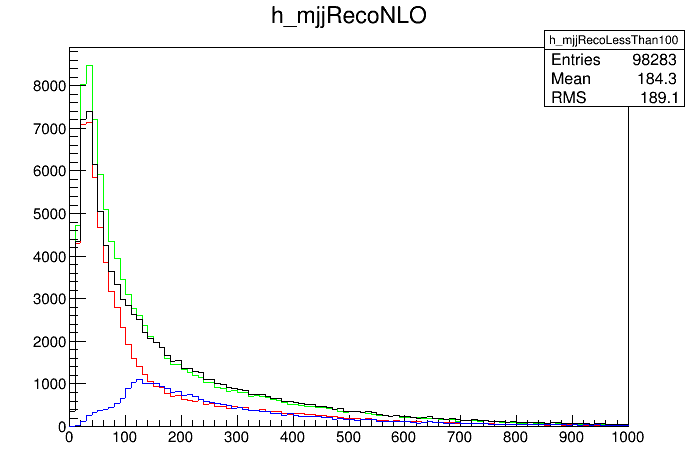
\includegraphics[width=0.6\textwidth]{../AN/Figs/WW_distribution}
\caption{ Distribution for $m_{jj}$ at RECO level for the merged WW sample.}
    \label{fig:WW}
\end{figure}




\subsection*{The Top sample}
In order to control the top quark background processes, the analysis is
performed in jet bins as described in Cap.~\ref{cap5}. The jet binning enhances the importance of logarithms of the jet \pt, spoiling the convergence of 
fixed-order calculations of the qq$\rightarrow$WW process and requiring the use of dedicated resummation techniques for an
accurate prediction of differential distributions~\cite{Meade:2014fca,Jaiswal:2014yba}.  
Since the \pt of the jets produced in association with the WW system is strongly correlated with its transverse momentum, 
\pt$^{WW}$,  the simulated qq$\rightarrow$WW events are reweighted  
to reproduce the \pt$^{WW}$ distribution from the \pt-resummed calculation.
A \ttbar  dilepton sample was also generated using \POWHEG v2. 
The cross sections of the different single top processes are estimated by the LHC Top Working group~\cite{singletop} at NLO.
The \ttbar cross section is also provided by the LHC Top Working group~\cite{topxsec}, and it is computed at NNLO, with NNLL soft gluon resummation. 


\subsection*{The DY sample}\label{sec:DY}
For the Drell-Yan backgrounds we use two different sets of samples. 
For the opposite flavore analysis (Sec~\ref{sec:OF}), selecting events with an
electron and a muon, a dedicated sample in which only the
$Z/\gamma^{*}\rightarrow{}\tau\tau\rightarrow{e\mu\nu\nu}$ decay is simulated.
For the same flavor analysis (Sec.~\ref{sec:SF}), in which pairs of electrons
or muons are selected, a soup of different $H_T$ binned DY samples is used. A
detailed study about this soup is given below.
Drell-Yan production of Z/$\gamma^{*}$ is generated using \MADGRAPH~\cite{Alwall:2014hca} and the cross section is scaled using a LO to NNLO k-factor equal to 1.23. 
Given the lack of MC statistics in the LO inclusive DY sample the
$H_\mathrm{T}$-binned samples are used. This helps increasing the MC
statistics especially in the VBF category of the same flavor analysis, which is characterized by large values of $H_\mathrm{T}$.
The LO inclusive sample is used for events with $H_\mathrm{T} < 100$\GeV and it has been merged to the other samples selecting events with $H_\mathrm{T}$ below 100\GeV using the parton level information. The cross sections of those samples have been scaled applying the LO to NNLO k-factor. In Fig.~\ref{fig:DY_HT} the $H_\mathrm{T}$ distribution of the sample after the merging is reported, showing a smooth transition between different $H_\mathrm{T}$ samples.
\begin{figure}[htbp]
\centering
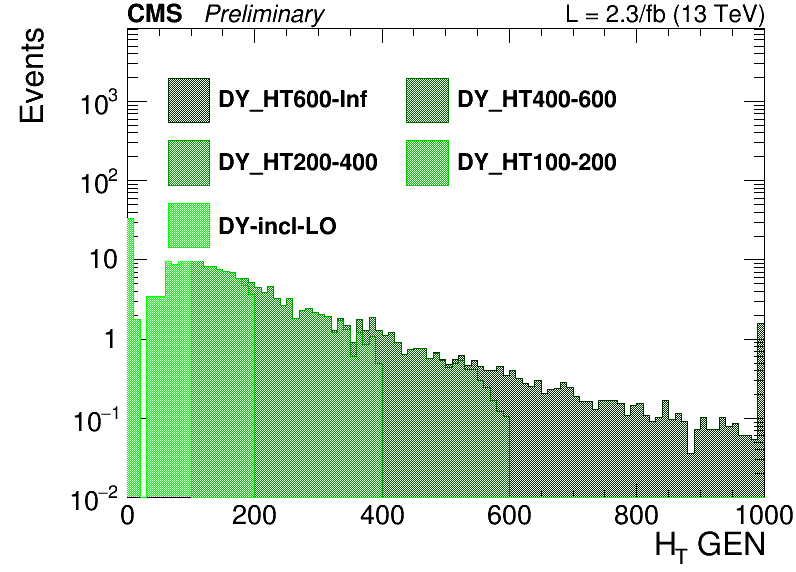
\includegraphics[width=0.6\textwidth]{../AN/Figs/log_c_incl_HTGen.png}
\caption{
    $H_\mathrm{T}$ distribution for the merged DY sample.}
    \label{fig:DY_HT}
\end{figure}
To further check the correct behaviour of the $H_\mathrm{T}$ binned samples we compared them to the inclusive LO sample, selecting only the events with a generator level $H_\mathrm{T}$ above 100\GeV. The comparison is done in a control region with two same flavor leptons with $\pt > 20$\GeV and $\mll > 50$\GeV, showing very good agreement between the two samples. The distributions of some variables are shown in Fig.~\ref{fig:inclDYvsHT}
\begin{figure}[htbp]
\centering
\subfigure[\mll]{
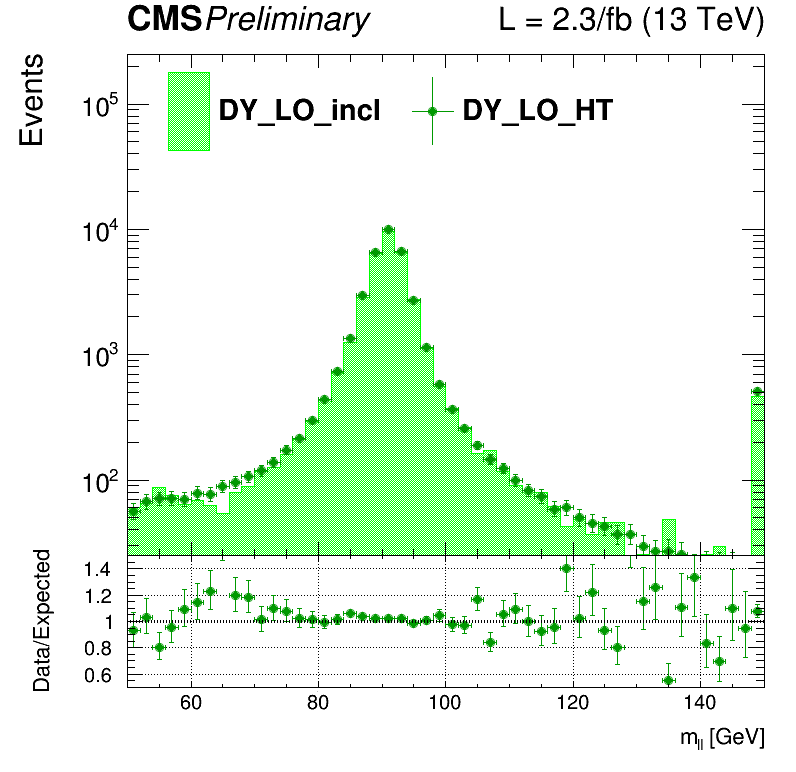
\includegraphics[width=0.45\textwidth]{../AN/Figs/DY/inclLOvsHT/log_cratio_dyee_13TeV_mll.png}
}
\subfigure[\ptll]{
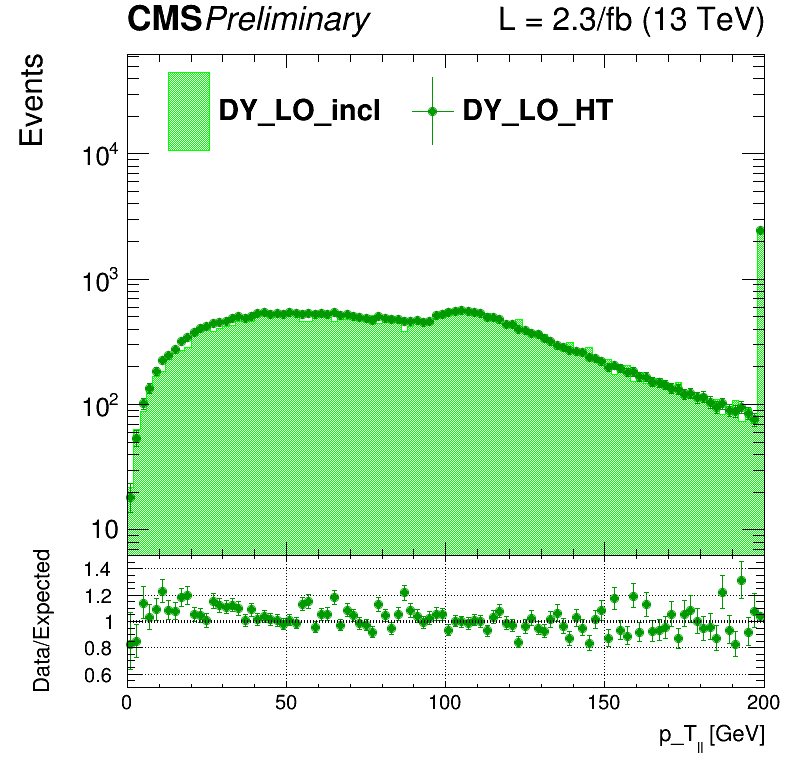
\includegraphics[width=0.45\textwidth]{../AN/Figs/DY/inclLOvsHT/log_cratio_dyee_13TeV_ptll.png}
}
\\
\subfigure[$\eta$ of leading lepton]{
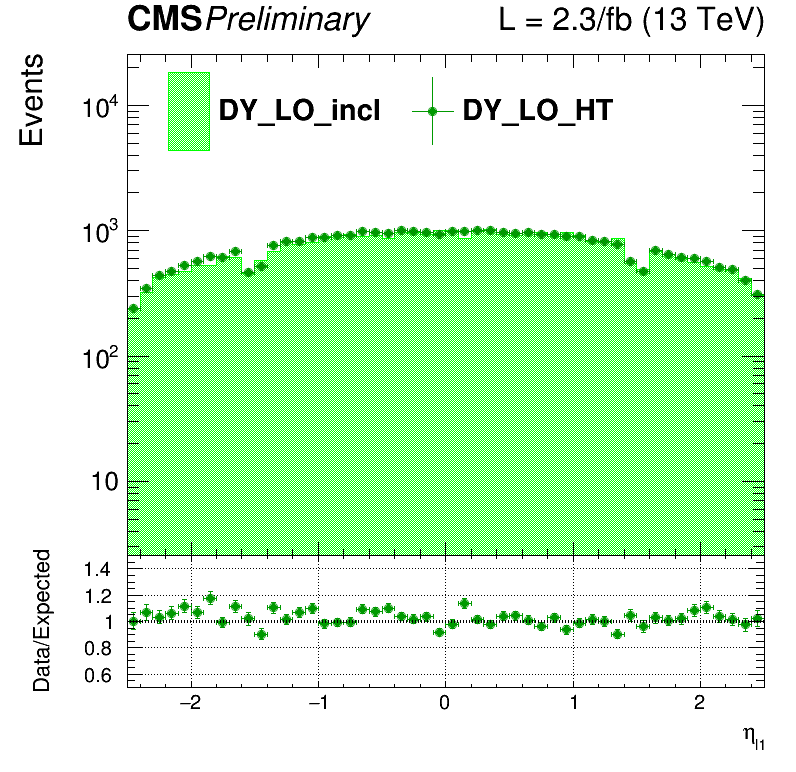
\includegraphics[width=0.45\textwidth]{../AN/Figs/DY/inclLOvsHT/log_cratio_dyee_13TeV_eta1.png}
}
\subfigure[$\eta$ of trailing lepton]{
\includegraphics[width=0.45\textwidth]{../AN/Figs/DY/inclLOvsHT/log_cratio_dyee_13TeV_eta2.png}
}
\caption{
    Comparison between the inclusive LO DY sample and the $H_\mathrm{T}$ binned samples.}
    \label{fig:inclDYvsHT}
\end{figure}
To check the differences between the LO inclusive sample and the NLO sample simulated with \MCATNLO, the two samples have been compared in a same flavor control region and some variables of interest are shown in Fig.~\ref{fig:LOvsNLO}. The control region is defined requiring two same flavor leptons with $\pt > 20$\GeV and with $\mll > 50$\GeV.
\begin{figure}[htbp]
\centering
\subfigure[\mll]{
\includegraphics[width=0.45\textwidth]{../AN/Figs/DY/LOvsNLO/log_cratio_dyee_13TeV_mll.png}
}
\subfigure[\ptll]{
\includegraphics[width=0.45\textwidth]{../AN/Figs/DY/LOvsNLO/log_cratio_dyee_13TeV_ptll.png}
}
\\
\subfigure[$\eta$ of first lepton]{
\includegraphics[width=0.45\textwidth]{../AN/Figs/DY/LOvsNLO/log_cratio_dyee_13TeV_eta1.png}
}
\subfigure[number of jets]{
\includegraphics[width=0.45\textwidth]{../AN/Figs/DY/LOvsNLO/log_cratio_dyee_13TeV_njet.png}
}
\caption{
    Comparison between the LO and NLO DY samples.}
    \label{fig:LOvsNLO}
\end{figure}
The simulated samples are generated with distributions for the number of pileup interactions
that are meant to roughly cover, though not exactly match, the conditions expected for the
different data-taking periods. 
In order to factorize these effects, the number of true pileup interactions from the simulation truth is reweighted to match the data. 
The re-weighting is propagated automatically to both the in-
time pile up and the out-of-time one.
In Fig.~\ref{Fig:pu}, the effect of this reweighting on a sample enriched in Drell-Yan events is shown.
In order to select this sample, 
events with two electrons with \pt$> 25$~\GeV for the leading one and  \pt$>
13$~\GeV for the trailing one, are selected only if  $|\mll - m_Z| < 10$~\GeV. 

\subsection*{Other processes} Other multiboson processes, such as WZ,ZZ, and VVV (V=W/Z), are generated with a\MCATNLO and normalized
to the cross section obtained at NLO in generation.
The cross sections for the remaining processes were directly obtained from the generator itself.


\section{Study of the Interference effects}
\label{sec:interference}
When a resonance $X$, with a non negligible width is considered, it is important to take into account also the interference effects both with the \WW background, in case of same initial and final state, and with the Higgs boson off-shell tail. 
The interference is taken into account both when the new signal X is produced via gluon-gluon fusion and when it is produced via vector-boson-fusion:
the effects are shown in ~\ref{fig:X300} and  \ref{fig:Int_VBF_GEN} for the two different production mechanisms.  The contribution of the interference of the high mass resonance $X$ with the \WW background and with the Higgs boson have opposite sign and partially cancel out. This cancellation effect is different for different values of the resonance mass.
The interference contribution is in general non negligible and it is included in the fit, Sec~\ref{StatIn}. \\
\begin{figure}[htbp]
\centering
\subfigure[Mass 300 \GeV.]{
\includegraphics[width=0.55\textwidth]{../AN/Figs/Interference_higgsLHEmass300_cuts_nocuts.png}
}
%\subfigure[Mass 400 \GeV.]{
%\includegraphics[width=0.48\textwidth]{../AN/Figs/Interference_higgsLHEmass400_cuts_nocuts.png}
%}
%\\
\subfigure[Mass 700 \GeV.]{
\includegraphics[width=0.55\textwidth]{../AN/Figs/Interference_higgsLHEmass700_cuts_nocuts.png}
}
\subfigure[Mass 1500 \GeV.]{
\includegraphics[width=0.55\textwidth]{../AN/Figs/Interference_higgsLHEmass1500_cuts_nocuts.png}
}
\caption{Distribution of for the $X$ mass resonance, produced via gluon-gluon fusion for different masses. In black the high mass signal. In red the interference between the high mass signal and the Higgs boson. In blue the interference between the high mass signal and the background. In green the total interference i.e. high 
mass signal, Higgs bison and background. }
    \label{fig:X300}
\end{figure}


\begin{figure}[htbp]
\centering
\subfigure[Mass 300 \GeV]{
\includegraphics[width=0.55\textwidth]{../AN/Figs/Inter_VFB/Interference_higgsLHEmass300_cuts_nocuts.png}
}
\subfigure[Mass 1500 \GeV]{
\includegraphics[width=0.55\textwidth]{../AN/Figs/Inter_VFB/Interference_higgsLHEmass1500_cuts_nocuts.png}
}
\caption{Distribution of for the $X$ mass resonance, produced via vector-boson-fusion fusion for different masses. In black the high mass signal. In red the interference between the high mass signal and the Higgs boson. In blue the interference between the high mass signal and the background. In green the total interference i.e. high 
mass signal, Higgs bison and background.}
    \label{fig:Int_VBF_GEN}
\end{figure}
} 
{\chapter{Event Reconstruction}
In the search of high mass in $W^+W^-$ channel, leptons (specifically, electrons or muons and neutrinos) and jets are searched for to select signal events.
The reconstruction of such objects follow standard algorithms and procedure which have been
developed by the experiment. In this chapter the reconstruction of the interested objects are described.

\section{The Particle Flow}
\label{PFt}
The algorithm for the event reconstruction is called Particle Flow (PF)~\cite{CMS-PAS-PFT-09-001}. Its goala is to reconstruct all stable particle that emerge from a hadron-hadron collision, such as muons, electrons, photons, charged hadrons, and neutral hadrons. The PF technique uses all the informations coming from the 
CMS sub-detectors and combines them to obtain: type of particle, direction, momentum, and energy.
The reconstruction of charged particles is done from the hits in the silicon tracker that is immersed in a uniform magnetic field of 3.8 T. 
Therefore, a transverse momentum precise measurement can be done down to about 150 MeV.
The photon and electron reconstruction is performed using the high resolution and granularity of the ECAL together with the excellent tracking system. This combination provides a very good energy resolution for such particles. Muons are reconstructed in the muon chambers together with the tracking system.
The reconstruction of charged-particles in the tracker, energy clusters in the calorimeters and muons in the muon chambers are the first steps of the PF. The informations are then connected to each others, making blocks of elements which are topologically compatible.
Starting by blocks, the candidates particle (PF Candidates) are fully reconstructed and identified as:
\begin{itemize}
\item Muons: the combination of a track in the tracker and a track in the muon system gives rise to a PF muon. The corresponding track is removed from the block after the identification.
\item Electrons: a charged-particle track is linked and one or more ECAL clusters (if presents)
\item Charged hadrons: PF charged hadrons are obtained from the remaining tracks. Tracks 
are linked to ECAL and HCAL clusters, and the deposited energy is determined taking into
account the momentum of the track.
\item Photons and Neutral hadrons: PF photons are given by ECAL clusters not compatible with charged-tracks; PF
neutral hadrons instead are given by unaccounted HCAL deposits.
\end{itemize}
After that, once the list of PF Candidates is defined, the PF jets are clustered. At the end the PF MET is evaluated as  the opposite of the transverse momentum-vector sum over all reconstructed PF Candidates.

\section{Tracking}
\subsection*{Hit reconstruction in the pixel and strip detector}
The first step of the reconstruction process is referred to as local reconstruction~\cite{Chatrchyan:2014fea}.  It consists of the clustering of zero-suppressed
signals above specified thresholds in pixel and strip channels into hits,  and then estimating the cluster positions and their uncertainties defined in a local
orthogonal  coordinate  system ($u$, $v$) in  the  plane  of  each  sensor (pixel and strip). 
The  hit reconstruction in the pixel detector and in the the strip detector is described below:
\begin{itemize} 
\item In the pixel detector: in the data acquisition system of the pixel detector, zero-suppression is performed in the
readout chips of the sensors, with adjustable thresholds for each pixel.  This pixel readout threshold 
is set to a single-pixel threshold corresponding to an equivalent charge of 3200
electrons.  Offline, pixel clusters are formed from adjacent pixels, including both side-by-side
and corner-by-corner adjacent cells.  Each cluster must have a minimum charge equivalent to
4000 electrons
\item In the strip detector:  the clusters are seeded by any channel passing zero-suppression that has a charge at least a
factor of three greater than the corresponding channel noise. Neighbouring strips are added
to each seed, if their strip charge is more than twice the strip noise. 
A cluster is kept if its total charge is a factor five larger than the cluster noise.
The position of the hit corresponding to each cluster is determined from the charge-weighted
average of its strip positions, corrected for the  Lorentz drift.
\end{itemize}

\subsection*{Track reconstruction}
Different algorithms are used in CMS for track reconstruction,~\cite{Chatrchyan:2014fea, Adam:2005cg}.
All   methods   use   the   reconstructed positions (hits) of the passage of charged
particles inside the CMS silicon detectors to determine the
trajectories of the charged tracks and therefore measure their directions and momenta.  
The Combinatorial Track Finder (CTF) is the main standard algorithm and proceeds in three steps:
\begin{itemize} 
\item Seeding:  pairs of hits, that are compatible with the interaction region above a lower
$p_T$ limit, are considered as possible candidates of
charged tracks.  Pixel hits provide the best track
seeding, given their three-dimensional position in formation and lower occupancy.  
\item Finding: is based on a standard Kalman  Filter  pattern  recognition  approach.
The  track trajectory  is  extrapolated  to  the  neighboring tracker  layers, starting form the seeded parameters.
Compatible  hits  are  assigned to the track. 
The Kalman Filter, a  succession of  alternating  prediction  and  filtering  steps, 
updates the track parameters at each steps with new hits.
 The updated tracks are assigned a quality and only the best ones are kept for further propagation. 
\item Fitting: the  final  estimate  of  the   parameters  of
each  track  helix  is  completed  in  the  last  steps
applying again the Kalman Filter for the trajectory fitting.  Each trajectory is refitted using a
least-squares fit. In the central region, $|\eta|<1$, the $p_T$ resolution is better than 1\%  for tracks with $p_T<10\%$. At higher $p_T$ resolution worsens approximately as $\Delta (1/p_T) \sim 0.2$ TeV$^{-1}$.
\end{itemize}
The  reconstruction  of  single  muons  with  the
CTF  algorithm  is  almost  fully  efficient  over  the whole acceptance range.
Electrons, being charged particles, can be reconstructed through the standard track reconstruction.  However,  as electrons lose energy primarily through bremsstrahlung,  rather than ionization,  large energy losses are common.  
 The energy loss distribution is highly non-Gaussian, and therefore the standard Kalman filter is not appropriate.
Electron candidates are reconstructed using the  information from the tracker but also from
the ECAL, Sec~\ref{ler}. 
For charged hadrons the reconstruction is more problematic due to their nuclear
interactions  in  the  tracker  material. 


\subsection*{Primary-vertex reconstruction}
The goal of primary-vertex reconstruction~\cite{Speer:927395}  is to measure the location, and the associated
uncertainty, of all proton-proton interaction vertices in each event, including the ``signal'' vertex
and any vertices from pileup collisions, using the available reconstructed tracks.  
It consists of three steps: 
\begin{itemize} 
\item  selection of the tracks;
\item clustering of the tracks that appear to originate from the same interaction vertex;
\item fitting for the position of each vertex using its associated tracks.
\end{itemize}
Track selection involves choosing tracks consistent with being produced promptly in the primary interaction region, 
by imposing requirements some requirements~\cite{Chatrchyan:2014fea} on the significance and on the $\chi^2$.
The selected tracks are then clustered on the basis of their z-coordinates at their point of closest approach to the centre of the beam spot  using a
\textit{deterministic annealing} (DA) algorithm~\cite{726788}. 
The algorithm proceeds in a way that is analogous to that of a physical system approaching a state of minimal energy through a series of
gradual  temperature  reductions. 
The z-coordinates  of  the  points  of  closest  approach  of  the tracks to the centre of the beam spot are $z_i^T \pm \sigma_i^Z$.
 The tracks must be assigned to some unknown number of vertices at positions $z_k^V$.
The tracks can be associated with more than one vertex, with probability $p_{i,k}$ that is  the probability of the
assignment of track $i$ to vertex $k$ in a large ensemble of possible assignments.
 The most probable vertex positions at ``temperature'' T (like in the calculations in statistical mechanics) is,
\begin{equation}
F=-T \sum_{i}^{\# \; tracks} p_i \, \log \sum_{k}^{\# \, vertices} \rho_k  \exp [-\frac{1}{T} \frac{(z_i^T-z_k^V)^2}{(\sigma_i^z)^2}  ]
\end{equation}
 relative to the positions of the vertices $z_k^V$ with vertex weights $\rho_k$ (the weights are variable, but the sum is always constrained
to unity).
The DA algorithm is initiated at a very high temperature with a single vertex and $T$ is gradually decreased.
This procedure traces the global minimum of $F$ from high to low temperature.
The number of vertices increases as the temperature falls, and rises each time the minimum of $F$ turns into a saddle point at lower temperatures. 
The DA process thereby finds not only positions and assignments of tracks to vertices but also the number of vertices.
In Fig.~\label{Fig:pu} is shown the distributions of the number of vertices in a Drell-Yan sample.
\begin{figure*}[htbp]
\centering
\includegraphics[width=0.6\textwidth]{../AN/Figs/nvertices.png}
\caption{
    Distributions of the number of vertices in a Drell-Yan enriched sample
    (Z$\rightarrow{}ee$) in
    data}
    \label{Fig:pu}
\end{figure*}




\section{Calorimeter clusters}
The purpose of the clustering algorithm in the calorimeters are~\cite{Sirunyan:2017ulk}:
\begin{itemize} 
\item detect and measure the energy and direction of stable neutral particles such as photons and neutral hadrons;
\item separate these neutral particles from charged hadron energy deposits;
\item reconstruct and identify electrons and all accompanying bremsstrahlung photons;
\item help the energy measurement of charged hadrons for which the track parameters were not determined accurately,
which is the case for low-quality and high $p_T$ tracks.
\end{itemize}
For the PF event reconstruction, a  specific clustering algorithm was developed. 
The clustering is performed separately in each subdetector: ECAL (barrel and endcaps) and HCAL (barrel and endcaps)
In the algorithm, first, \textit{cluster seeds} are identified   as cells with an energy larger than a given seed threshold, and
larger than the energy of the neighbouring cells. Second, \textit{topological clusters} are grown from the seeds by aggregating cells with at least a corner in common with a cell already in the cluster.
After an expectation-maximization algorithm based on a Gaussian-mixture mode to
reconstruct the clusters within a topological cluster is used.
The Gaussian-mixture model postulates
that the energy deposits in the M individual cells of the topological cluster arise from N Gaussian energy deposits where N is the number of seeds. 
The expectation-maximization algorithm is an iterative algorithm with two steps at each iteration.
During the first step, the parameters of the model are kept constant and the parameters of the model are determined during the second step in an analytical maximum-
likelihood. 
The energy and position of the seeds are used as initial values for the parameters of the corresponding 
Gaussian functions and the expectation maximization cycle is repeated until convergence.

\section{Link algorithm}
A given particle is, in general, expected to give rise to several PF elements in the various CMS
subdetectors. The reconstruction of a particle therefore first proceeds with a
link algorithm that connects the PF elements from different subdetectors.
The link between a track in the central tracker and a calorimeter cluster is established:
the track is first extrapolated from its last measured hit in the tracker to
 the ECAL at a depth corresponding to the expected maximum of a typical longitudinal electron shower
profile, and to the HCAL at a depth corresponding to one interaction length.  
The track is linked to a cluster if its extrapolated position is within the cluster area, defined by the union of the
areas in the HCAL and the ECAL in $(\phi, \eta)$ plane. 
After, Calorimeter cluster-to-cluster links are sought between HCAL clusters and ECAL clusters.
Charged-particle tracks may also be linked together through a common secondary vertex, for
nuclear-interaction reconstruction.
Finally, a link between a track in the central tracker and information in the muon detector is
established to form global and tracker muons, Sec~\ref{ler}.\\

In each PF block, the identification and reconstruction sequence proceeds as,
\begin{itemize} 
\item first, muon candidates are identified and reconstructed and the
corresponding PF elements (tracks and clusters) are removed from the PF block.  
\item The electron identification and reconstruction follows. Energetic and isolated photons, converted or un-
converted, are identified in the same step.  The corresponding tracks and ECAL or preshower
clusters are excluded from further consideration
\item The remaining elements in the block are then subject to a cross-identification of charged hadrons,
neutral hadrons, and photons, arising from parton fragmentation, hadronization, and decays
in jets. 
\end{itemize}

\section{Jet Energy Calibration}
The purpose of the jet energy calibration is to relate, on average, the energy measured for the
detector jet to the energy of the corresponding true particle jet.  A true particle jet results from
the clustering (with the same clustering algorithm applied to detector jets, Sec.~\ref{jetr}) of all stable particles
originating from the fragmenting parton, as well as of the particles from the underlying event
(UE) activity. 

The jet energy calibration is related,  on average, on the energy measured in
the detector to the true energy of the corresponding final state particle jet or parton jet.
From the clustering  of all stable particle, a true particle jet results. The correction is applied as
a multiplicative factor C to each component of the raw jet four-momentum vector, $p_{\mu}^{raw}$, as:
\newline
\begin{equation}
p_{\mu}^{corr}=C \cdot p_{\mu}^{raw} \; ,
\end{equation}
where correction factor $C$ is composed of the offset correction $C_{offset}$ , the MC calibration
factor $C_{MC}$, and the residual calibrations $C_{rel}$ and $C_{abs}$ for the relative and absolute
energy scales, respectively. The various components are applied in sequence:
\newline
\begin{equation}
C=   C_{offset} ( p_{\mu}^{raw}) \cdot  C_{MC} (p_T',\eta) \cdot C_{rel}(\eta) \cdot  C_{abs} (p_T'') \; ,
\end{equation}
\newline
where $p_T'$ is the transverse momentum of the jet after applying the offset correction and $p_T''$ is the transverse momentum 
of the jet after all previous corrections. The details of each component are:
\begin{itemize}
\item $C_{offset}$: a energy offset is produced by the pileup of multiple proton-proton collisions and by electronic noise.
The goal of the offset correction is to subtract, on average, the unwanted
energy from the jet. For the offset correction estimation, the Jet Area Method has been used. 
An average $p_T$-density $\rho$ per unit area is estimated, for each event. 
The key element for this approach is the jet area $A_j$.
A very large number of infinitely soft four-momentum vectors are artificially added in the event and clustered
by the jet algorithm together with the true jet components. The other important quantity for the pileup subtraction is the $p_T$ density $\rho$, which
is calculated with the $k_T$ jet clustering algorithm with a distance parameter R$=$0.6.
The quantity $\rho$ is defined on an event-by-event basis as the median of the distribution of
the variable $p_{Tj}  /A_j$ , where j runs over all jets in the event, and is not sensitive to the
presence of hard jets. Therefore, the event-by-event and jet-by-jet offset correction can be defined as,
\begin{equation}
  C_{offset}= (p_T^{raw}, A_j ,\rho )=1- \frac{(\rho -\langle \rho_{UE}  \rangle )\cdot A_j }{p_T^{raw}} \; ,
\end{equation}
where $\langle \rho_{UE}  \rangle$ is the $p_T$-density component due to the UE and electronics
noise, and is measured in events with exactly one reconstructed primary vertex (no pileup).
\item $C_{MC}$: is based on the simulation and corrects the energy of the reconstructed
jets such that it is equal on average to the energy of the generated jets (GenJets). The
GenJets reconstruction algorithm is identical to the one applied to the data.
The response variable, $R=p_T^{reco}/p_T^{gen}$, in each bin of the GenJet transverse momentum $/p_T^{gen}$, is recorded as jet $p_T^{reco}$.
The average correction in each bin is defined as,
\begin{equation}
  C_{MC}(p_T^{reco})= \frac{1}{\langle R \rangle } \; ,
\end{equation}
\item $C_{rel}$: the goal of the relative jet energy scale correction is to make the jet response flat versus $\eta$. 
This is achieved by employing a Tag and Probe technique, selecting dijet
events in data. The size of this residual correction is of the order of 2-3\% in the
central $\eta$ region, while it goes up to about 10\% in the forward region.
\item $C_{abs}$: the goal of the absolute jet energy scale correction is to make the jet response flat versus $p_T$.
Once a jet has been corrected for $\eta$ dependence, it is corrected back to particle
level.
\end{itemize}
Each type of correction has uncertainties arising from many different sources.
These sources are categorized as: physics modeling in MC, MC modeling of true detector response and potential biases in the methodologies used to estimate the corrections. In CMS more than 16 such sources of uncertainties have been identified. Several are
related and can be combined into groups that are relative to the absolute scale, relative
scale, extrapolation in $p_T$ , pileup, jet flavor and time stability.

\section{Pileup subtraction}
At the LHC,  at each bunch crossing there are of the order of 20 minimum bias proton-proton interactions, which pollute any interesting hard events with many soft particle. The kinematic measurements for jets will be adversely affected by pileup (PU), with resolution and absolute energy measurements
suffering significantly: in fact for the  neutral particles is not possible distinct primary vertex that corresponds to a single
proton-proton interaction,  and most jet measurements are carried out with calorimeters, which do not have the angular
resolution needed to reconstruct the original primary vertex.\\
An event-by-event, and jet-by-jet, pileup subtraction approach, which performs the corrections after the jet finding,  has been out~\cite{Cacciari:2007fd}
carried out.  It is based on:
\begin{itemize}
\item the jet’s susceptibility to contamination: it is embodied in the jet area A measured on $\eta$ and $\phi$. The jet area is different for each jet and depends on the details of its substructure, and practical measurement of the jet areas is carried out using the FastJet package. 
Given a suitable definition of jet area, the modification of a jet’s $p_T$ by diffuse noise can be shown to be,
\begin{equation} 
\Delta p_T=A\rho \pm \sigma \sqrt{A} -L \:, \qquad \langle L \rangle=\mathcal{O}(\alpha_S \times A \rho \ln \frac{p_T}{ A \rho}) \:,  
\end{equation} 
where $\rho$ is the level of diffuse noise that  corresponds to the amount of transverse momentum added to the event per unit area (at LHC is around 
10-20 GeV~\cite{Sjostrand:2003wg}): the first term is therefore the geometrical contamination of the je
t and is associated with an uncertainty (second term) because of fluctuations in the noise from point to point in the event.
$L$  accounts for the occasional loss (or the even more occasional gain) of part of the jet’s contents,
due to the fact that jets can be modified when clustered in the presence of diffuse noise, as some
of the particles originally clustered into one jet can instead end up in a different one. \\
If the fluctuations are small, $\sigma << \sqrt{A} \, \rho$, the measured $p_T$ for each jet $j$ using the subtraction is given by,
\begin{equation} 
p_{T,j}^{sub}=p_{T,j} -A_J \rho \: ,
\end{equation} 
where $A_j $ is the jet area. This equation provides a correction to the jet’s scalar transverse
momentum.
\item The second ingredient in carrying out the subtraction is the estimate of $\rho$ for each event.
The principal difficulty in estimating the amount of noise is that of distinguishing the noise component from the large amounts of $p_T$ deposited by the hard event.
The $\rho$ value  for each even can be estimated~\cite{Cacciari:2007fd}  taking the median value of this distribution in the event: 
\begin{equation} 
\rho= median \; [\{\frac{p_{T,j}}{A_j}\}]  \: ,
\end{equation} 
\end{itemize}
The above pileup subtraction procedure is valid if: 
\begin{itemize}
\item The pileup noise should be independent of $\eta$ and $\phi$.
\item The radius $R$ of the jet algorithm should be no smaller than the typical distance between minimum bias particles, otherwise the extraction of
 $\rho$ from the median will be biased by the large amount of empty area not associated with jets
\item The number of pileup jets should be much larger than the number of jets from the hard interaction. 
\end{itemize}



\section{Lepton reconstruction and identification}
\label{ler}
\subsection*{Electron reconstruction and identification}
The combination of tracker and ECAL information is used for electrons reconstruction.
The electrons, emerging from a collision, when interact with the silicon tracker, radiate bremsstrahlung photons that reaches the ECAL with a significant spread in the azimuthal direction $\phi$. These energy deposites measured in ECAL are the starting point of the electrons reconstruction algorithm. They are associated in clusters and in superclusters (clusters of clusters) that take into account the spread in the $\phi$ direction of the bremsstrahlung energy, Fig.~\ref{clustering}.
When   superclusters are identified, the reconstruction algorithm tries to match them to track seeds. The  track seeds are identified as pairs or triplets of hits in the inner tracker layers. The electrons trajectories are reconstructed using a dedicated modeling that take in account  energy
loss in the tracker layers via  bremsstrahlung radiation: non-Gaussian contributions to the event-by-event fluctuations 
of the calorimetry and tracking measurements are introduced due to the bremsstrahlung radiation.   
\begin{figure}
\centering
\includegraphics[scale= 0.2]{../Cap4/clustering}
\caption{EM cluster spread in $\eta$ and $\phi$.}
\label{clustering}
\end{figure}
A preselection is applied to solve ambiguous cases where several tracks are reconstructed. It is based on matching
between the GSF track and the supercluster in $\eta$ and $\phi$. To achieve a good resolution the electron supercluster must
be inside the ECAL acceptance volume, that meaning  $\eta<$ 2.5, and outside the ECAL barrel-endcap
overlap region, 1.4442 $<\eta<$ 1.566.
Several identification variables are used to achieve a good discrimination. These variables are:
\begin{itemize}
\item $\Delta \eta_{trk,SC}$ and $\Delta \phi_{trk,SC}$, that measure the spacial matching between the track
and the supercluster.
\item $\sigma_{in,in}$ that measures the width of the ECAL supercluster in the $\eta$ direction. It is the calorimeter shower shape.
\item H/E: is the ratio among the energy deposit in the HCAL tower and the energy of the seed supercluster.
\item $|$1/E - 1/p$|$ the difference of 1/E measured in ECAL and 1/p measured in the tracker.
\item Number of missing hits
\item $d_{xy}$ and $d_z$, impact parameters with respect to the reconstructed primary vertex (PV).
\item $\gamma \to e^+ e^-$ veto based on missing hits in the inner layers of the tracker.
\end{itemize}
Different selections on the above variables define different working points (WP). The cuts are also different for electrons in
the ECAL barrel or in the endcap. The WPs are:
\begin{itemize}
\item Tight WP: this corresponds to an average 70\% selection efficiency for electrons with
$p_T >$ 20 GeV. This working point is used where backgrounds are very large. The
$X \to WW$ high mass analysis has large backgrounds like W+jets, where the second lepton is a ``fake'', i.e. a jet identified as an isolated lepton. 
So, in this analysis we use Tight WP for electrons. On the top of that, we apply more cuts to make the electron id selection Trigger safe.
\item Medium WP: the average efficiency is about 80\% for electrons with $p_T>$ 20
GeV. This is also a good starting point for measurements of W and Z cross-sections.
\item Loose WP: this working point is used only for very clean final states. The average efficiency is about 90\%.
\item Veto WP: generally, this is not used for signal selection. However, it is found to
be useful for extra lepton veto counting of electrons. The average efficiency is about 95\%.
\end{itemize}
Selected electrons are also required to pass the isolation criteria that include a pile-up mitigation correction based on the electron effective 
catchment area. The isolation variable is computed for each electron as,
\begin{equation}
ISO^{Rel}_{EA\; corrected}=[\sum_{ChH}(p_T) + max(0, \sum_{Ph}(p_T)) +\sum_{NH}(p_T)  -\rho EA ]/p_T^{electron} \, ,
\end{equation}
where $ChH$ is an index which runs on the charged hadrons, $Ph$ on the photons, $NH$ on the neutral hadrons, $\rho$ is the pile up energy
density and $A$ is an effective area. The sum is done in a isolated cone of $\Delta R<$ 0.4 around the electron direction.
The identification and isolation criteria used for the $X \to WW$ analysis are summarised in Tab.~\ref{IDe}.

\begin{table}
\centering
\begin{tabular}{|lll|}
\hline
Observable & Barrel (EB) cut &Endcap (EE) cut\\
\hline
$|\Delta \eta_{trk,SC}|$  &0.00308  & 0.00605 \\
$|\Delta \phi_{trk,SC}|$ & 0.0816   &0.0394\\
$\sigma_{in,in}$ &0.011& 0.031\\
H/E & 0.060& 0.065\\
$|$1/E - 1/p$|$ & 0.013 &0.013\\
Number of missing &1&1\\
$|d_{xy}|$ &0.05&1\\
$|d_z|$ &1&1\\
conversion veto& true&true\\ 
\hline
$ISO^{Rel}_{EA\; corrected}$&0.0588 & 0.0571\\
\hline

\end{tabular}
\caption{Electron identification criteria for the Tight working point and isolation requirements.}
\label{IDe}
\end{table}

\subsection*{Muon reconstruction and identification}
Muons produced in the interaction point can pass through all the detector, with a negligible energy loss, and give a signal in the muon chamber.
Their loss of energy is very negligible. 
Muons are thus reconstructed both in the silicon tracker and in the external muon chambers. 
The reconstruction starts from the measurements of DT, CSC and RPC sub-detectors. The reconstructed track in the muon spectrometer is called
Stand-alone Muon.
Muon tracks are also reconstructed In the inner silicon tracker. Seeds are
built using two or three consecutive hits in the pixel and or in the strip detector. 
The pattern recognition is performed starting from these seeds and proceeding layer by layer,
with an iterative technique based on the Kalman Filter.
At the end of this algorithm, a track fit is performed and the track parameters are updated. The identified
tracker track is then combined with a given Stand-alone Muon track in order to construct
a global track, which defines a Global Muon. A global fit is performed for each pair of
tracks reconstructed in the inner tracker and in the muon system. If more than one track
matching the stand-alone track is found, then the one giving the best $\chi^2$ in the global fit
is chosen. Exist a second approach that consists in considering all tracker tracks with $p_T>$ 0.5 GeV as
potential muon candidates. These tracks are extrapolated to the muon system taking
into account the magnetic field. If at least one muon segment (a short track stub made of
DT or CSC hits) matches the extrapolated tracks, the corresponding tracker track is
identified as a Tracker Muon.
Quality requirements are applied to ensure a good quality of the reconstruction:
the tracker track has to be reconstructed from at least 5 tracker layers with hits;
\begin{itemize}
 \item at least one hit must be present in the pixel detector;
 \item least one hit must be present in the muon detector;
 \item least one muon chamber hit should be included in the Global Muon track fit;
 \item normalized $\chi^2$ of the Global Muon track fit should be less than 10;
 \item muon track reconstructed in the tracker must have a distance to the primary
vertex (PV) smaller than 2 mm in the transverse plane and smaller than 5 mm in
the longitudinal direction.
\end{itemize}
The requirements are summarized in Tab.\ref{IDm}

\begin{table}
\centering
\begin{tabular}{|ll|}
\hline
Observable& Value Cut\\
\hline
Is global muon                        & true              \\ 
Is PF muon                            & true              \\ 
Tracker layers with measurements      & $>5$              \\ 
Number of valid pixel hits            & $>0$              \\ 
Number of valid muon hits             & $>0$              \\ 
Number of matched muon stations       & $>1$              \\ 
$\chi^2$ /ndof                        & $<10$             \\ 
$d_{xy}$ (PV)                         & < 0.2 cm          \\ 
$d_z$ (PV)                            & < 0.5 cm          \\ 
\hline
\end{tabular}
\caption{Muon identification and isolation requirements..}
\label{IDm}
\end{table}
For the analysis goals, the muon are expected to be isolated, as the  produced by W boson decay. Indeed, prompt muons are expected to be isolated in the event, contrary to non-prompt muons that are generally produced within jets and characterized by many
nearby particles. Muon coming from $W$, and so from $X$, must be isolated and they are requested to pass an isolation
criterion which also icludes a PU mitigation correction called ``$\Delta \beta$ correction''.
The isolation variable is therefore sensitive to the
pileup and a correction is needed in order to ensure its independence and robustness on
the number of simultaneous interactions. The isolation variable used is,
\begin{equation} 
ISO^{Rel}_{\Delta \beta}=[\sum_{ChH}(p_T) + max(0, \sum_{Ph}(p_T) -0.5 \times \sum_{ChHUP}(p_T)) ]/p_T^{electron} \, ,
\end{equation}
where $ChH$ is the charged hadrons, $Ph$ is photons and $ChHPU$ is charged
hadrons not coming from the primary vertex.  The sum is performed in a cone of 0.4 units in $\Delta R$ around the muon.
A bias in the muon $p_T$ is introduced by the imperfect knowledge
of the magnetic field and the effect of the material distribution. In addition the $p_T$ measurement is sensitive to the alignment of the tracker and
muon chambers. To estimate the muon $p_T$ scale and resolution are used different method. For $p_T<100$ GeV, the  events with two muon arising from the $J/\Psi$ and Z
resonance decays are used to correct the $p_T$ scale. Above, so in the high $p_T$ regime, are used cosmic ray muons.

\section{Jet reconstruction and identification}
\label{jetr}
Jets are the experimental signature of quarks and gluons produced in the hadron collision. They result from the parton  hadronization and they play a major in a hadronic collider where final state with jets have very large cross-section. The technique used for jet reconstruction is the Particle Flow.
Using the particle-flow algorithm described in Sec.~\ref{PFt}, the  jets are reconstructed by clustering of the  four-momentum vectors of candidates: the information from relevant CMS sub-detectors are used to identify and to reconstruct all visible particles in the event, as
 muons, electrons, photons, charged hadrons, and neutral hadrons. 
The momentum and spatial resolutions of jet identified with PF technique, are greatly improved respect to jet identified with only the calorimeter information. Indeed the use of the tracking detectors allows a better resolution of $p_T$ for the charged particles.
The sequential and iterative jet clustering algorithm, that combine four-vectors of input particles, are used to form the jets.
A ideal jet clustering algorithm should have the following features:
\begin{itemize}
\item infrared safety: infrared singularity should not appear in the perturbative calculation;
\item collinear safety: collinear singularities must not appear in the perturbative calculations;
\item invariance under boosts: the algorithm should find the same solutions independently
by boosts in the longitudinal direction.
\item order independence: the algorithm should find the same jets at parton, particle, and detector level;
\item straightforward implementation: the algorithm should be straightforward to imple-
ment in perturbative calculations.
\end{itemize}
The jet algorithm should also follow these  experimental criteria
\begin{itemize}
\item detector independence: the performance of the algorithm should be as independent from the detector;
\item minimization of resolution smearing and angle biases: the algorithm should not
amplify the inevitable effects of resolution smearing and angle biases;
\item stability with luminosity: jet finding should not be strongly affected by pileup;
\item efficient use of computing resources: minimum of computer time consumption;
\item maximal reconstruction efficiency: the algorithm should efficiently identify all jets;
\item ease of calibration and use: algorithm should not obstruct to the reliable calibration and and to be straightforward to implement.
\end{itemize}
Jet definition is not unique, being the parton not a well-defined object, so several
approaches for jet clustering are available. Two main algorithms for clustering have been developed. The ``conical recombination''
where jets are defined as dominant directions of energy flow.  The second class is called sequential recombination and it works by defining a distance
between pairs of particles, performing subsequent recombinations of the pair of closest
particles and stopping when all resulting objects are too far apart. The standard algorithms adopted by
CMS are the SISCone in the conical recombination class, and the $k_t$, Cambridge-Aachen (CA) and anti-$k_T$ algorithms, Sec~\ref{rico_jet}.\\
\newline

\subsection*{Jets in $X \to WW$}
The jets collection is made by clustering the reconstructed particles known as the Particle Flow
Candidates in the CMS software. The reclustering algorithm used is the anti-kt algorithm with
a distance parameter equal to 0.4. Pileup mitigation is done with the Charge Hadron Subtraction  algorithm 
which removes charged particles coming from pileup vertices before
clustering.
The Jet Energy Corrections  that are applied to correct the reconstructed jet energy back
to the true energy of the final state particles.  To reject jets originating
from calorimeter or readout electronics noise the loose working point of the PF Jet Identification is applied. 
This analysis selects a jet by the selection cut as,
\begin{equation}
 p_T^{Jet} > 30 GeV \: , |\eta| < 5.0 \: .
\end{equation}
The various distributions of jet after correction are shown at Fig.~\ref{jetFig}
\begin{figure}
\centering
\includegraphics[scale= 0.5]{../Cap4/jetFig}
\caption{The jet kinematic distributions:.}
\label{jetFig}
\end{figure}

\section{b-jet identification}
To identify the b jets  the properties that characterize hadrons are used
containing the quark b.
In fact these hadrons have a relatively large mass, around 5 GeV, and a long average life, about 1.5 ps. Given that they can
have an impulse of several tens of GeV, the distance that they travel in the detector
it is of the order of:
\begin{eqnarray}
\delta &\approx& t_{medio} \: v \approx \gamma \: \tau \: \beta  \: c  \nonumber \\
 &\approx& 10 \cdot 1.5 \cdot 10^{-12} \mbox{s} \cdot 1 \cdot 3 \cdot 10^8 \: \mbox{m/s}   \nonumber \\
 &\approx& 5  \mbox{mm.} \end{eqnarray}
A distance that can be measured since the accuracy of the position of the
secondary vertices is $\sim$100 $\mu$m.
The CMS collaboration has developed different algorithms to identify the jets coming from
  quarks b (b-tag algorithms). Each of these algorithms is characterized
from a certain efficiency of signal identification (jets from b quark) and from the probability of
reject the background (jet not from b quark), which in general depend on the transverse impulse,
$p_T$, and from the pseudorapidity  of the jet. To build an observable (or discriminator) which distinguishes 
the jets originated by b from those originating from light quark 
is used to reconstructed objects such as, traces, vertices and leptons. 
Some algorithms simple but reliable use a single observable in input, while others
more complexes combine different ones to generate the discriminator. Each algorithm
produces, in output, a single value of the discriminator for each jet of the event.
The first step in identifying of b-jets is the reconstruction of all the jets present in the
the event. As mentioned, the CMS collaboration uses for jet reconstruction
the anti-$k_T$ algorithm, applied to Particle Flow objects. However the algorithms of
identification require a sample with well reconstructed and high purity traces.
Therefore further cuts to the traces of the jet are applied. First of all, to reduce
the number of traces reconstructed incorrectly, a transverse pulse is required
greater than 1 GeV and at least two signals in the silicon pixel detector. Then, at 
least eight signals per track must be present with a fit that has a
 $\chi^2$/d.o.f. $<$5, where d.o.f. it is the number of degrees of freedom of the fit. It also applies
also a selection on the impact parameters: this is used to increase
the fraction of well reconstructed traces and to reduce the contamination due to long life particles like neutral kaons.
The transverse distance $d_{xy}$ and longitudinal $d_z$ between the trace and the primary vertex
are required to be smaller than 0.2 cm and 17 cm respectively.
In Fig.~\ref{bj}  it is
was a schematic representation of the parameters used in the identification
of the b jets.
\begin{figure}
\centering
\includegraphics[scale= 0.5]{../Cap4/btag}
\caption{Cluster spread in $\eta$ and $\phi$.}
\label{bj}
\end{figure}
\subsection*{Impact Parameter algorithm}
The impact parameter (IP) of a track respect to the primary vertex, can be used to distinguish 
the hadrons b decay  respect to background tracks (prompt). The IP is calculated in three dimensions 
thanks to the excellent resolution of the pixel detector.
The impact parameter has the same sign of the product scalar between the direction of the
jet and the distance of the primary vertex from the nearest point of the trace. The traces
produced by particles due to the decay of a hadron with a long average life
they have a positive value of IP, while for the traces originated from the primary vertex
(prompt) the IP will be both negative and positive.
The variable used as observable is the significance of the parameter of
pact, S$_{IP}$, defined as the relationship between IP and its estimated uncertainty. There
significance of the impact parameter can therefore be used as a discriminant  between b and non-b jets.
The Track Counting (TC) algorithm orders in significance
IP traces of jets, from the highest to lowest. There are two different versions of this algorithm that
they are distinguished on the basis of which significance value is taken into consideration:
Track Counting High Efficiency (TCHE) uses the S$_{IP}$ of the second track , while the Track Counting High Purity (TCHP) use the third.
A natural extension of the TC algorithms is the combination of the several tracks impact points. 
This is implemented in the Jet Probability (JP) and Jet algorithms
B Probability (JBP). The former uses an estimator for the likelihood he evaluates
which may be the probability that all traces associated with a jet come from
from the vertex of primary interaction. The estimator of likelihood, P$_{jet}$, is defined
such as,
\begin{equation}
P_{jet}=\Pi \cdot \sum_{i=0} ^{N-1} \frac{(-\ln \Pi)^i}{i!} \qquad \mbox{con} \qquad \Pi= \prod_{i=0} ^{N}\mbox{max}(P_i, 0.005)  \mbox{,}\end{equation} 
where N is the number of traces considered and P  the probability that the track is
originated in the primary vertex.
Instead the JBP algorithm gives more weight to the tracks (up to a maximum of four) than
they are connected to a jet from b; these are identified as they have a high level
value of the significance of IP.

\subsection*{Secondary Vertex identification}
The presence of a
secondary vertex in the event and related variables  can be used
to discriminate jets coming from a quark b respect to the others. The main variables associated with the secondary vertex are the distance, the flight direction
with respect to the primary vertex, the mass and the energy of the particles associated to the traces
secondary. To identify a secondary vertex it is required that:
\begin{itemize}
\item shares less than 65\% of its traces associated with the primary vertex and
the significance of the radial distance between the two vertices is beyond 3$\sigma$;
\item the flight distance of each candidate is in a cone with $\Delta R <$0.5 around
to the direction of the jet;
\item the secondary candidates who have a distance over
per 2.5 cm above the primary vertex, both a mass compatible with
that of K$_0$ or that in any case exceeds 6.5 GeV.
\end{itemize}
The Simple Secondary Vertex (SSV) algorithm uses as a discriminating variable 
the significance of the flight distance, given by the distance ratio of
flight with its uncertainty. Similar to the TC algorithm, there are two versions
of SSV: High Efficiency (SSVHE) which uses vertices to which they are associated at least
two tracks, and High Purity (SSVHP) that requires at least three tracks.
There are more complicated algorithms that consider the secondary vertices together with the
information on the average life. This makes it possible to construct a discriminant
even when there is no secondary summit, increasing efficiency in terms of
to SSV; two of these algorithms are the Combined Secondary Vertex (CSV) and the
Combined Secondary Vertex Version 2 + Inclusive Vertex Finder (CSVV2IVF).
The difference between the two is that the CSV algorithm uses to reconstruct the vertices share information from jets while the CSVV2IVF algorithm uses
all the tracks present in the event.
Moreover, in general, there are some variables that are not very related to each other and that
they can be used as good discriminators that are:
\begin{itemize}
\item the category of vertices;
\item the significance of the flight distance in the transverse plane;
\item the mass of the vertex;
\item the number of vertex tracks;
\item the ratio between the energy carried by a track and the other jet tracks;
\item the pseudorapidity of the track;
\item the number of traces in the jet.
\end{itemize}

\subsection*{b-tag performance in $X \to WW$ analysis}
In order to assess which tagger and working point are performing better, we have calculated
the signal significance for different taggers and working points in the 0 and 1 jet categories,
which are the most sensitive to the dominant gluon fusion production mode. The significance
has been computed running the full analysis but including only the systematic uncertainties
associated to the b tagging scale factors. The results are shown in Tab.~\ref{btt}.
The results show that the usage of CMVA (loose WP) or Deep CSV (medium WP) leads to a
comparable signal significance in the combined 0+1 jet category. The CMVA tagger with loose
WP has been found to be the best option for the analysis, given the good performance and the
nice agreement that has been observed between data and MC, Fig.~\ref{cmvaT} and  Fig.~\ref{cmvaD}.
\begin{figure}
\centering
\includegraphics[scale= 0.3]{../Cap4/btt}
\caption{Signal significance for different taggers and working points in the 0 and 1 jet categories. The significance for the combination of the 0 and 1 jet categories is shown as well. Only
the systematic uncertainties associated to the b tagging scale factors are taken into account for
the significance evaluation.}
\label{btt}
\end{figure}

\begin{figure}
\centering
\includegraphics[scale= 0.4]{../Cap4/cmvaT}
\caption{CMVA discriminator for jets above 30 GeV (a) and between 20 and 30 GeV (b) in a
top enriched control region, after applying the scale factors. The top background normalization
is scaled to match data. The systematics band comprises only the uncertainties related to the b
tagging scale factors.}
\label{cmvaT}
\end{figure}

\begin{figure}
\centering
\includegraphics[scale= 0.4]{../Cap4/cmvaD}
\caption{CMVA discriminator for jets between 20 and 30 GeV (a) and above 30 GeV (b) in the
Z enriched control region. The normalization of the DY background is scaled to match data.
The systematics band comprises only the uncertainties related to the b tagging scale factors..}
\label{cmvaD}
\end{figure}

\section{The Missing Transverse Energy}
The longitudinal momentum (along the beam axis) in the collision is not known, so the measurement of the total missing
energy is impossible.
However the initial transverse momentum, carried by the incoming partons, is zero, so in the final state of the collision, for the conservation of the momentum
components, the sum of momenta of all the particles must be zero.
If a missing transverse momentum, $\vec{p_T^{miss}}$, in the transverse plane is present, it is the evidence of invisible particles, such as neutrinos particles predicted by some BSM models.
The $\vec{p_T^{miss}}$ is defined as,
\begin{equation}
\vec{p}_T^{\: miss}= -\sum_{PF\: Objs} \vec{p}_T^{\:PF \: Obj} \: ,
\end{equation}
where the sum extends over all the PF objects. The $\vec{p_T^{miss}}$ is the  negative
vectorial sum of transverse momenta of all reconstructed PF objects, and its module is called missing transverse energy, $E_T^{miss}=|\vec{p_T^{miss}}|$.
As inefficiencies of the tracking algorithm, minimal thresholds in the calorimeter energy
estimation, and nonlinearities of the energy response of the calorimeters for hadronic parti-
cles can introduce a bias in the $\vec{p_T^{miss}}$ determination, a correction is applied by propagating
to the $\vec{p_T^{miss}}$ sum the jet energy corrections,  in according as,
\begin{equation}
\vec{p}_T^{\:miss \: correction}= \vec{p}_T^{\:miss} -\sum_{Jets}( \vec{p}_T^{\:Corr} -\vec{p}_T) \: ,
\end{equation}
where the superscript JEC refers to corrected jets.
To estimate the $E_T^{miss}$  systematic uncertainty we have considered the following sources:
\begin{itemize}
\item jet $p_T$;
\item jet resolution;
\item muon  $p_T$;
\item electron $p_T$;
\item unclustered energy.
\end{itemize}
The $E_T^{miss}$ has been computated varying each of these uncertainties and added in quadrature the
differences with respect to the nominal value. For the $\phi$ uncertainty has been taken as the largest
$\phi$ variation.
The distributions of various  $E_T^{miss}$ variables, in the electron-muon channel, are shown in Fig.~\ref{met}
\begin{figure}
\centering
\includegraphics[scale= 0.8]{../Cap4/met}
\caption{The  $E_T^{miss}$ filters efficiencies for 35.9 fb$^{-1}$ of 2016 data. The common requirements for
the distributions before filters (solid histogram) and after filters (black points) are the trigger
and two tight leptons.}
\label{met}
\end{figure}

\section{Fake Lepton Background Estimation}
Lepton fake rates are measured as a
function of the lepton $p_T$ and $\eta$, in a single lepton triggered sample. The test of the method and
systematic errors are described below.
In the analysis
the primary source of background from misidentification is W+Jets. QCD multi-jet and hadronic top backgrounds
are also present at much smaller level. Events in which W bosons are produced in association
with jets give rise to background to WW events when a jet is misidentified as a lepton. These
events contain a real lepton and real missing energy from the W decay. With the jet misidentified 
as a lepton, the W+Jets events have two identified leptons, missing energy, and no other
significant event characteristics. As a result, the W+Jets events cannot be readily suppressed
by event selection. This background is particularly important at low $p_T$.
The estimation of the fake lepton contribution is based on the ``fakeable objet'' data-driven
method and provides a measurement of the yield and the kinematic distributions of fake background. 
It is a general technique, applicable to any physics analysis in which particle level
selection criteria are used to suppress background. The method can be used with any number
of final state particles and is independent of the event selection.
The fundamental idea of the fakeable objet method is simple: select a control sample of events
enriched in the background being estimated, and then use an extrapolation factor to relate these
events to the background in the signal region. The method is data-driven provided the control
sample is selected in data, and the extrapolation factor is measured with data. For background
arising from particle misidentification, the extrapolation is done in particle identification space
($p_T$ and $\eta$ ) of the lepton. The control sample is defined using a looser particle selection criteria
that are chosen such that the rate of misidentification is increased. The extrapolation factor
relates background misidentified with this criteria, to background misidentified as passing the
full particle selection of the signal region.
} 
{\chapter{Analysis strategy}


%{
\textit{%As described in Sec.~\ref{NSP}, the research of  new resonance $X$ is one of the mail goals of LHC. With a energy achieved of 13 TeV in the center of mass and the data collected in 2016, it is possible to lead searches in a vast range of mass. One of the main final state channel in in a couple of $W^+W^-$ bosons.
In this chapter the $X \to \mathrm{W^+W^-}\to2\ell2\nu$ analysis using 2016 data is reported. To increase the sensitivity of this search, the signal must be selected in the most efficient way by reducing the
presence of the backgrounds with a similar signature: the selection criteria are described in detail. I have participated at all stages of the analysis selection (signal simulation, categorization, background estimation, etc.)  and I have been responsible for the whole analysis.} 
%The ATLAS experiment has been done this kind of searches using the early 2016 statistic, 13.2 fb$^{-1}$ and the results are shown in Fig.~\ref{ATLAS-CONF-2016-074_fig}.
%With the full 2016 statistic, approximately $\sim 36$ fb$^{-1}$ is possible to investigate a wide range of masses and, if will be no evidence of high mass signal, is possible to set  tight upper limits on the possible cross section.

\section{Overview of the fully leptonic analysis }\label{sec:AnalysisStrategy_Intro}
The analysis strategy for the high mass search in the $X \to \mathrm{W^+W^-}\to2\ell2\nu$ final state must take into account the production modes of the new scalar, the main backgrounds, and the interference among the different processes. 

The main production mode for a Higgs-like particle over the all mass spectrum is the gluon-gluon fusion process. 
However the ratio of the VBF cross-section to the gluon-gluon fusion cross-section increases with $m_\mathrm{X}$ (see Fig.~\ref{prod}), making the VBF production mechanism more and more important.\\

Among the SM processes that have the same final state of the signal or a similar one the most important are non-resonant WW production, top production, Drell-Yan. The WW production is an irreducible background and needs to be determined together with the signal in the fit. To estimate the other background processes, control regions are defined on data and compared to simulation. \\
The events are first divided according the flavour in the final state: 
\begin{itemize}
\item opposite-flavour final state, $e^{\pm} \mu^{\mp}$,
\item same-flavour final state, $e^+ e^-$ and  $\mu^+ \mu^-$. 
\end{itemize}
In the opposite-flavour final state four different jets categories are defined: the 0-jet, the 1-jet, the 2-jet and the VBF, Sec.~\ref{sec:OF}. 
In the same-flavour final state only the VBF category is considered. Indeed, only the VBF selection cuts are sufficiently tight to reduce the  overwhelming Z plus jets background to a manageable level, Sec.~\ref{sec:SF}. The jets categories improve the sensitivity of the analysis, because each category has different contributions from signal production modes and backgrounds.

The signal is interpreted in terms of the EWK singlet and MSSM models as described in Sec~\ref{NSP}. The Higgs boson width and lineshape is reweighted at generator level according to the parameters defined in the model. The interference effects between the signal produced via gluon-gluon fusion, the WW background also from gluon-gluon fusion, and SM Higgs boson, are expected to change the shape of the signal distribution and have been fully taken into account. 
A similar treatment is also applied for the interference between high mass signal produced via VBF, the WW plus two quarks background (emerging from the same initial state) and the SM Higgs generated with VBF production mechanism. In general, the interference becomes more and more important as the mass of $X$ increase and it is studied in detail in Sec~\ref{sec:signalModel}.
Finally, the interference between the $\mathrm{W^+W^-}\to2\ell2\nu$ and $\mathrm{ZZ}\to2\ell2\nu$ is negligible due to the different phase space characteristic of these processes.




\section{Main Background processes}
\label{anbkg}
Inside the SM that are several processes that have the same or a similar final state of the signal. The most important background processes contributing to this final state are non resonant $q\bar{q} \to W^+ W^-$, the top production ($t\bar{t}$ and single-top) and the Drell-Yan process. 
Other backgrounds are due to $W$+jets events, where a jet is misidentified as a lepton, and multibosons events. 
All these processes have been simulated with Monte Carlo generators and the simulation details have been discussed in Sec~\ref{MSsample}.
A detailed description of these background processes is given below:
\begin{itemize}
\item \textit{Non-resonant WW} ($q\bar{q} \to W^+ W^-$): this background is characterized by a final state identical to the signal, however the lepton kinematics for signal and $q\bar{q} \to W^+ W^-$ processes is rather different.
For the signal process, the W bosons originate from a spin-0 particle decay
and their spins must therefore be antiparallel, implying that the charged leptons produced 
in their decays appear preferentially in the same hemisphere~\cite{Ellis:2012wg}. In contrast,
there is no preferential spin direction in the background case. For this reason the
azimuthal angle difference between the two leptons is on average smaller for signal
than for background, resulting in a smaller dilepton invariant mass in the former case. The most relevant Feynman diagram of the process is shown below.
\begin{figure}[h]
\centering
\vspace{0.5cm}
\includegraphics[scale= 0.9]{../Cap5/nnr_WW}
\end{figure}
\item \textit{Top} ($t\bar{t}$ and single-top): the $t\bar{t}$ events give a signal-like signature if both decays $t \to Wb$ are followed by $W \to \ell \nu$.  In such a case, in fact, there are two leptons and missing transverse energy,  plus two jets (from the hadronization of the $b$ quark) in the final state. This process is especially important when the signal is produced via VBS or when the signal is associated with jets coming from initial or final state radiation. The single-top production is characterized by the presence of a $W$ boson and a top quark, so after the top decay, again by two W's, but only one b-jet. Following, some examples of Feynman diagrams for the top background: the $t\bar{t}$ in (a) and (b) diagrams, the single-top in (c).
\begin{figure}[h]
\centering%
\subfigure[]%
{\includegraphics[scale= 0.3]{../Cap5/ggtt_t}} \qquad 
\subfigure[]%
{\includegraphics[scale= 0.3]{../Cap5/qqtt_s}} \qquad 
\subfigure[]%
{\includegraphics[scale= 0.5]{../Cap5/st_bg}}
\end{figure}
%\newpage
\item \textit{Drell-Yan}: the Drell-Yan process is defined as the annihilation of a quark-antiquark pair into a lepton-antilepton pair. This process is described at leading order by
the two  shown Feynman diagrams. %These amplitudes are proportional to the fine structure constant $\alpha \sim 1/137$.
This kind of background is particularly important for the same flavour final state of the signal
\begin{figure}[h]
\centering
\vspace{0.5cm}
\includegraphics[scale= 0.7]{../Cap5/dy}
\end{figure}

\item \textit{W+jet}: this background is charaterized by a $W$ boson, decaying in $\ell \nu$, produced in association with a jet. If a fake lepton arise from the misidentified jet, these events have  the same final state of the signal (two leptons and missing-transverse-energy), Sec~\ref{fk}. 

\item \textit{Other}: other background processes involve multibosons production, such as $WZ/W\gamma^*$, $ZZ^*$ and $Z\gamma$ with $\gamma$ conversion.

\end{itemize}
The main background processes, the \WW production and the top production, are estimated using data. 
Instrumental backgrounds arising from non-prompt leptons in $W+$jets production and mis-measurement of $E_T^{miss}$ in Drell-Yan events are also estimated from
data. The contribution from W$\gamma^*$  is estimated partly from data. The
contribution of other sub-dominant backgrounds is obtained directly from simulated samples. The different data-driven background estimations are explained in the following sections. 
%More precisely top and  Drell-Yan backgrounds normalizations have been extracted
%directly from data-simulation comparison in specific control regions enriched in either one
%or the other background separately for the different events categories, using the rateParam feature of the combine package~\cite{combine}.


\section{Fake Lepton Background Estimation}
\label{fk}
Lepton fake rates are measured as a
function of the lepton $p_T$ and $\eta$, in a single lepton triggered sample. The test of the method and
systematic errors are described below.
In the analysis
the primary source of background from misidentification is W+Jets. QCD multi-jet and hadronic top backgrounds
are also present at much smaller level. Events in which W bosons are produced in association
with jets give rise to background to WW events when a jet is misidentified as a lepton. These
events contain a real lepton and real missing energy from the W decay. With the jet misidentified 
as a lepton, the W+Jets events have two identified leptons, missing energy, and no other
significant event characteristics. As a result, the W+Jets events cannot be easily suppressed
by event selection. This background is particularly important at low $p_T$.
The estimation of the fake lepton contribution is based on the ``fakeable object'' data-driven
method and provides a measurement of the yield and the kinematic distributions of fake background. 
It is a general technique, applicable to any physics analysis in which particle level
selection criteria are used to suppress background. The method can be used with any number
of final state particles and is independent of the event selection.
The fundamental idea of the fakeable objet method is simple: select a control sample of events
enriched in the background being estimated, and then use an extrapolation factor to relate these
events to the background in the signal region. The method is data-driven provided the control
sample is selected in data, and the extrapolation factor is measured with data. For background
arising from particle misidentification, the extrapolation is done in particle identification space
($p_T$ and $\eta$ ) of the lepton. The control sample is defined using a looser particle selection criteria
that are chosen such that the rate of misidentification is increased. The extrapolation factor
relates background misidentified with this criteria, to background misidentified as passing the
full particle selection of the signal region.



\section{Lepton Efficiencies from Tag and Probe Method}
\label{TP}
One of the well established data-driven approach for measuring the particle efficiencies is the
so called Tag and Probe method. The Tag and Probe method uses a known mass resonance (e.g. $J/\Psi$, $Z$) to select particles of the desired type, and probe the efficiency of a particular
selection criterion on these particles. In general the “tag” is an object that passes a set of very
tight selection criteria designed to isolate the required particle type. Tags are often referred
to as a “golden” electrons or muons and the fake rate for passing tag selection criteria should
be very small. A generic set of the desired particle type (i.e. with potentially very loose selection 
criteria) known as “probes” is selected by pairing these objects with tags such that the
invariant mass of the combination is consistent with the mass of the resonance. Combinatoric
backgrounds may be eliminated through any of a variety of background subtraction methods
such as fitting, or sideband subtraction. The definition of the probe objects depend on the specifics of the selection criterion being examined. The simple expression to get the efficiency %as a function of $p_T$ and $\eta$ 
is given below:
\begin{equation}
\epsilon=\frac{N_{Pass}^{Probes}}{N_{Pass}^{Probes}+N_{Fail}^{Probes}}
\end{equation}

\subsection*{Electrons} 
The   Tag and Probe is used here to get the identification and isolation efficiency of electrons. In this case, the Tag is a
well identified and isolated electron which also passes an electron trigger. 
Once the Tag electron is selected then another object that pass the kinematic electron selection, Tab.~\ref{IDe}, is searched for. 
The invariant  mass of the Tag and the Probe electron pair is reconstructed and must be in window around the Z boson mass. 
After that, to compute the efficiency, the Probe electron is required  to pass the identification tight working point. 
This procedure is performed for the data and the MC samples. 
Once data and MC efficiencies have been calculated, the electron scale factors are estimated as the ratio among the data and MC efficiencies.  
These scale factors are calculated as a function of $p_T$ and $\eta$ and used to correct the difference in efficiencies between data and MC in the analysis. 
%The Pile-Up reweighting is also applied on MC during the computation of efficiencies. 
%A MC truth matching has also been applied in case of the computation using simulation. 
%In principle, there are two methods to estimate the efficiencies.
%The first one is the \textit{counting method} and the other one is the \textit{fitting method}. 
%The counting method is used when there  are small backgrounds, instead  the fitting method instead when the backgrounds are 
%In order to take into account the effect of DY background in the efficiency estimation,  a fitting method has been used. 
%Tag and Probe pairs are  selected in Z mass window of 60 to 120 GeV.
%If there exist more than one pair then the one whose invariant mass closer to Z pole mass has been selected.
%The efficiencies have been computed as a function of $p_T$ and $\eta$ of electron.
%For signal fitting, MC templates are derived from the simulated sample in the Z mass range 60 to 120 GeV in  $p_T$ and $\eta$ bins.
%The MC Templates are then smeared using Gaussian function. For the background fitting a function, that is combination of
%an exponential function and an error function, has been used.
%The exponential decay distribution becomes
%active at high mass beyond the Z peak and the error function takes over at low masses due to
%threshold effect.
%A fit examples for all $p_T$ bins is shown in Fig.~\ref{ac}
%\begin{figure}
%\centering
%\includegraphics[scale= 0.5]{tpe}
%\caption{Fits for $p_T$ bin (35-50) GeV and $\eta$ in (-2.5,-2.0) bin.}
%\label{ac}
%\end{figure}

The electron efficiency is about 95\%, on the trigger plateau. 


\subsection*{Muons} 
The muon identification and isolation efficiency is also studied and compared to the prediction of MC in order
to understand if a correction is needed. The muon efficiency is obtained as
\begin{equation}
\epsilon_{\mu} = \epsilon_{TRK} \times \epsilon_{Tight} \times \epsilon_{ISO \; Tight} \; ,
\end{equation}
\newline
where $ \epsilon_{TRK}$ is the tracker  muon efficiency.  
The $ \epsilon_{Tight} $ is muon efficiency
under the assumption that the muon passes the kinematic selections summarized in  Tab.~\ref{IDm}.
The $\epsilon_{ISO \; Tight}$ is the efficiency of the isolation criteria under the assumption that the muon passes the same selection.
The $\epsilon_{Tight}$ and $ \epsilon_{ISO \; Tight}$ are determined  using the Tag and Probe method. 
The Tag muon is obtained by applying  the kinematic selections  and   the isolated muon trigger  with $p_T^{\mu}>20$ GeV.
The Probe muon  is requested to pass the kinematic selection and the isolation criteria.
%After that it is checked if the Probe muon is matched to the muon trigger. 
%In general the efficiencies are relatively high due to the lower cut on $p_T$ and the looser cut on
%isolation %in the double lepton trigger compared to single muon trigger. 
The efficiency value on the plateau is around 93\%-99\%.



\section{Data sample and Trigger used}

%\subsection*{Data sample}
%\subsection*{Data in CMS}
Data recorded in proton proton collisions at 13 TeV during all 2016 was used in the analysis, with a total integrated luminosity of  35.9 \fbinv.
%The data has been reprocessed in the reprocessing campaign characterized by the submission date \textit{03Feb2017} in CMS.
%In Table~\ref{tab:data} the different data streams used are presented. 
All runs are taken with a 25~ns LHC filling scheme and recorded in seven different periods, namely Run2016C, Run2016D, Run2016E, Run2016F, Run2016G, and Run2016H.
% \begin{table}
% \begin{center}
% \begin{tabular}{|l|l|}
% \hline
% Data Taking Era & Stream\\
% \hline
% \multirow{5}{*}{Run2016C} 	& SingleMuon  \\
%                                 & DoubleMuon \\
% 				& SingleElectron \\
%                                 & DoubleEG \\
% 				& MuonEG \\ \hline
% \multirow{5}{*}{Run2016D}       & SingleMuon  \\
%                                 & DoubleMuon \\
%                                 & SingleElectron \\
%                                 & DoubleEG \\
%                                 & MuonEG \\ \hline
% \multirow{5}{*}{Run2016E}       & SingleMuon  \\
%                                 & DoubleMuon \\
%                                 & SingleElectron \\
%                                 & DoubleEG \\
%                                 & MuonEG \\ \hline
% \multirow{5}{*}{Run2016F}       & SingleMuon  \\
%                                 & DoubleMuon \\
%                                 & SingleElectron \\
%                                 & DoubleEG \\
%                                 & MuonEG \\ \hline
% \multirow{5}{*}{Run2016G}       & SingleMuon  \\
%                                 & DoubleMuon \\
%                                 & SingleElectron \\
%                                 & DoubleEG \\
%                                 & MuonEG \\ \hline
% \multirow{5}{*}{Run2016H}       & SingleMuon  \\
%                                 & DoubleMuon \\
%                                 & SingleElectron \\
%                                 & DoubleEG \\
%                                 & MuonEG \\ \hline
% \hline 
% \end{tabular}
% %\vspace{0.5cm}
% \caption{Data samples used in the analysis. The total integrated luminosity corresponds to 35.9\fbinv.
% \label{tab:data}}
% \end{center}
% \end{table}


%\subsection*{Triggers path and  efficiency}
Events are required to fire one of the unprescaled single-electron, single-muon or
muon-electron triggers. Due to the rather high LHC instantaneous luminosity the
single-lepton triggers must have high HLT $p_T$ thresholds, otherwise the rate of these
triggers would be too large to be sustained. The double-lepton triggers allow the $p_T$
thresholds to be lowered while keeping a sustainable trigger rate.
%, thus maintaining a
%good sensitivity to the Higgs boson signal, for which the lepton  $p_T$ can be rather small.
The triggers used in this analysis are summarized in Table~\ref{tab:triggers}. 
%Since a final state with two leptons is searched for, both single and double lepton triggers are used. 
%For the electrons a combination of triggers is necessary to increase the statistics and to adjust the $p_T$ threshold requirement. 
\begin{table}
\begin{center}
\begin{tabular}{|l|l|}
   \hline
   Trigger name & HLT Threshold \\
   \hline
   
   SingleElectron & $p_T>$ 27 GeV  \\

   \hline
        
   SingleMuon   &  $p_T>$ 22 GeV  \\

   \hline
   
   MuonElectron       &  $p_T>$ 17 GeV  and 8 GeV  \\
   
   \hline
   
   DoubleMuon   & $p_T>$ 17 GeV  and 8 GeV  \\
      
   \hline
   
   DoubleElectron   &  $p_T>$ 23 GeV  and 12 GeV    \\
   
   \hline
\end{tabular}
\caption{Transverse momentum thresholds applied in the lepton triggers at the HLT
level. Double set of thresholds indicates the thresholds for each leg of the double lepton
triggers.}
\label{tab:triggers}  
\end{center}
\end{table}\\
\newline
The trigger efficiencies are calculated for leptons that pass the identification and isolation criteria.
In Fig.~\ref{Fig:trigger} the trigger efficiency for a gluon-gluon fusion signal with mass 300~\GeV is shown for electrons (left) and muons (right).
An average trigger efficiency greater than 99\% is found, as shown in Figure~\ref{Fig:triggerIntegral}. The triggers used in the analysis are summarized in Table~\ref{tab:triggers}. 
\begin{figure*}[htbp]
\centering
\begin{tabular}{cc}
%  \includegraphics[width=0.45\textwidth]{Figs/Trigger/ele.png} &
%  \includegraphics[width=0.45\textwidth]{Figs/Trigger/mu.png} \\
%  (a) electron & (b) muon \\
 \includegraphics[width=0.45\textwidth]{../AN/Figs/Trigger/ele1.png} &
 \includegraphics[width=0.45\textwidth]{../AN/Figs/Trigger/mu1.png} \\
 (a) electron 1st & (b) muon 1st \\
 \includegraphics[width=0.45\textwidth]{../AN/Figs/Trigger/ele2.png} &
 \includegraphics[width=0.45\textwidth]{../AN/Figs/Trigger/mu2.png} \\
 (c) electron 2nd & (d) muon 2nd \\
\end{tabular}
\caption{
      Trigger efficiency per event
      as a function of the lepton \pt
      for electrons (a) where leading lepton is an electron, 
      and (c) where trailing lepton is an electron, 
      and muons (b) where leading lepton is a muon, 
      and (d) where trailing lepton is an muon, 
      for a gluon fusion 300~\GeV MC sample.
      In this plots the other lepton not shown is
      integrated.
      An average trigger efficiency greater than 99\% is found.      
     }
    \label{Fig:trigger}
\end{figure*}
\begin{figure*}[htbp]
\centering
 \includegraphics[width=0.6\textwidth]{../AN/Figs/Trigger/triggW.png}
\caption{
      Trigger efficiency distribution for 
      four MC samples corresponding to masses of 300, 500, 1000 and 3000~\GeV.
      An average trigger efficiency greater than 99\% is found.
     }
    \label{Fig:triggerIntegral}
\end{figure*}



\section{Discriminating variable}
This analysis is a shape analysis, meaning that after applying selection cuts, the events are not simply counted, but rather an histogram of a discriminating variable is filled from the data and fitted with the sum of signal and background templates, and finally the signal yield is extracted.
In principle, the variable with the best discriminating power would be the invariant mass of
the four lepton system, however, due to the presence of the neutrinos, it can not be measured.
Usually, in the the Higgs boson to $WW \to 2\ell 2\nu $, the variables used in the analysis are:
\begin{itemize}
\item the transverse mass, $m_T^H$, defined as,  
\begin{equation}
 m_T^H = \sqrt{2p_{\rm T}^{\ell\ell}\MET(1-\mathrm{cos}\Delta\phi(\ell\ell, \ptvecmiss))}
\end{equation}
where $\Delta\phi(\ell\ell, \ptvecmiss)$ is the azimuthal angle between the dilepton momentum and \ptvecmiss;
\item the di-lepton mass, $m_{\ell \ell}$.
\end{itemize}
However, both $m_T^H$ and $m_{\ell \ell}$, are not sensitive to different
signal mass hypothesis. For this reason a new variable, the visible transverse mass,  $m_T^I$, has been used.
This variable, studied for this specific analysis, is defined as the invariant mass of the four momentum resulting from the sum of the
two leptons four-momenta and the missing four-momentum: 
\begin{equation}
 m_T^I = \sqrt{ (p_\mathrm{\ell\ell} + \MET)^2 - (\vec{p}_\mathrm{\ell\ell} + \ptvecmiss)^2 \; .}
\end{equation}
The distribution of all the variables defined above can be compared in 
Fig.~\ref{fig:mt_nocuts}, where it is visible the better power of $m_T^I$ in discriminating different mass hypotheses wth respect to  $m_T^H$ and $m_{\ell \ell}$. The usage of  $m_T^I$ also provides a good discriminating power between signal and background.
The effects of the interference (Sec~\ref{sec:interference}) for the discriminating variable  $m_T^I$  used in the analysis is shown in Fig~\ref{nocut_mti_700_sign}
The interference is not negligible and it will take in account as part of the signal during the fit.
\begin{figure}[htbp]
\centering
\subfigure[True generated mass]{
\includegraphics[width=0.45\textwidth]{../AN/Figs/Distribution_higgsLHEmass_cuts_nocuts.png}
}
\subfigure[$m_T^H$]{
\includegraphics[width=0.45\textwidth]{../AN/Figs/Distribution_mth_cuts_nocuts.png}
}
\\
\subfigure[$m_{\ell \ell}$]{
\includegraphics[width=0.45\textwidth]{../AN/Figs/Distribution_mll_cuts_nocuts.png}
}
\subfigure[$m_T^I$]{
\includegraphics[width=0.45\textwidth]{../AN/Figs/Distribution_mTi_cuts_nocuts.png}
}
\caption{
    Distributions of the generated mass (no possible reconstruction), $m_T^H$, $m_{\ell \ell}$ and  $m_T^I$
    variables for different $X$ mass hypothesis. It is clear that the most discriminating variable is $m_T^I$. }
    \label{fig:mt_nocuts}
\end{figure}

\begin{figure*}[htbp]
\centering
 \includegraphics[width=0.6\textwidth]{../Cap5/nocut_mti_700_sign}
\caption{ The $m_T^I$ distribution at generator level for a $X$ resonances at 700 GeV produced via gluon-gluon fusion. In red the interference between the high
mass signal and the Higgs boson. In blue the interference between the high mass signal
and the background. In green the total interference i.e. high mass signal, Higgs bison and
background.       }
    \label{nocut_mti_700_sign}
\end{figure*}
}
% 
%{\newpage
\section{Opposite Flavor final state}\label{sec:OF}
\subsection*{General overview}

The events are subdivided in signal and control regions. The signal events are expected to fill  mainly to first one. Instead the second one are expected to be fill 
up by backgrounds events and they are used to normalized the backgrounds shape.\\
\newline
To avoid a possible bias of the experimenter in the process of developing the analysis
strategy and optimizing the selection requirements, firstly a blind analysis has been performed
by defining a background-only sideband control region and only looking at data events
falling in such a region. Precisely, the control region is defined according to  selection
criteria that exclude the signal events. 
Data in the signal region, i.e.  were not examined until the event selection
criteria were settled, only relying on Monte Carlo simulations for what concerns signal. 
In this way, the analysis strategy has been decided looking at the simulated events. 
Only when data distributions in signal-depleted regions confirmed the robustness of the analysis, data in
signal region were inspected. For these reasons, the agreement between data and Monte Carlo was
checked on a sideband region.




\subsection*{Signal region}
The events are requested to pass single or double lepton triggers, and exactly one electron and
one muon are requested to be reconstructed in the event. 
One of the two leptons is requested to have a $p_T$ greater than 25 GeV , the other is
requested to have  $p_T$ greater than 20 GeV and both leptons are requested to be well identified
and isolated, to reject non-prompt leptons and leptons coming from QCD sources. To suppress
background processes with three or more leptons in the final state, such as ZZ, WZ, Z$\gamma$, W$\gamma$
or triboson production, no additional identified and isolated lepton with $p_T >$  10 GeV should
be reconstructed. The low dilepton invariant mass region dominated by QCD production of
leptons is not considered in the analysis and $m_{\ell \ell}$  is requested to
be higher than 50 GeV to reduce the SM Higgs boson ($m_H$=125 GeV)
contamination. A moderate cut on the missing-transverse-energy is applied (MET $>$ 20 GeV) due to the
presence of neutrinos in the final state. Since a high mass
signal is searched a cut on $m_T^I >$ 100 GeV is applied.
A cut on the transverse momentum ($p_T^{\ell \ell} >$30 GeV) and on the $m_T^H
>$ 60 GeV are applied against $DY\rightarrow{}\tau\tau$ background. 
Finally, against the top background, all jets above 20 GeV are requested not
to be identified as b-jets according to the cMVAv2 tagger, loose WP.
The full selection, defined as the ``WW opposite-flavour selection'', is summarized:

\begin{itemize}
\item Two isolated leptons with different charge and flavor ( $\mu^{\pm}
e^{\mp}$);
\item $p_T$ of the leading lepton $>$ 25 GeV;
\item $p_T$ of the trailing lepton $>$ 20 GeV;
\item Third lepton veto: veto events if a third lepton with $p_T  >$ 10 GeV;
\item  $m_{\ell \ell} >$ 50 GeV, to reduce H(125) contamination;
\item MET $>$ 20 GeV;
\item $m_T^I >$ 100 GeV;
\item $p_T^{\ell \ell} >$30 GeV;
\item  $m_T^H >$ 60 GeV;
\item  no b-tagged (cMVAv2 loose WP) jets with $p_T >$  20 GeV;
\end{itemize}
Events passing the ``WW opposite-flavour selection'' are categorized according to the jet
multiplicity, counting jets above 30 GeV, to enhance the sensitivity,
especially against the top background. 

\begin{itemize}
\item {\bf 0 jet}, no jets are required in the event;
\item {\bf 1 jet}, exacly 1 jet is required in the event;
\item {\bf 2 jet}, exacly 2 jets are required in the event and in addition the condition $\Delta \eta_{jj} < 3.5$ {\bf or} $m_{jj} <$ 500 GeV;
\item {\bf VBF}, exacly 2 jets are required in the event and in addition the condition $\Delta \eta_{jj} > 3.5$ {\bf and} $m_{jj} >$ 500 GeV;
\end{itemize}
where the 2 jet and VBF regions are mutually exclusive by construction.
To extract high mass boson signals in these four categories, the  strategy  is followed: the $m_T^I$ distribution is fitted as the sum of
signal and background templates. Different binnings have been chosen for the  $m_T^I$ distributions in the
different categories. The binning was chosen to have  at least 10
top Monte Carlo events in each bin of the template. The chosen bins are: 
\begin{itemize}
\item  {\bf 0/1/2 jet}, [100,150,200,250,300,350,400,450,500,550,600,650,700,750,800,900,1000,2000]
\item {\bf VBF}, [100,150,200,250,300,350,400,500,700,1000,2000]
\end{itemize}
where the first number represents the lower edge of the first bin while the other numbers represent the upper edges. The last bin is an overflow bin.
The  $m_T^I$ distributions for the signal regions are presented in the four categories in Figs.~\ref{fig:mti_sigOF_Un_log}.

\begin{figure}[htbp]
\centering
\subfigure[0 jet]{
\includegraphics[width=0.45\textwidth]{../Cap5/log_cratio_hwwhm_13TeV_of0j_mTi.png}
}
\subfigure[1 jet]{
\includegraphics[width=0.45\textwidth]{../Cap5/log_cratio_hwwhm_13TeV_of1j_mTi.png}
}
\\
\subfigure[2 jet]{
\includegraphics[width=0.45\textwidth]{../Cap5/log_cratio_hwwhm_13TeV_of2j_mTi.png}
}
\subfigure[VBF]{
\includegraphics[width=0.45\textwidth]{../Cap5/log_cratio_hwwhm_13TeV_ofVBF_mTi_VBF}
}
\caption{Unblinding distributions  $m_T^I$ in the signal region for 0, 1, 2 and VBF categories. The signal hypothesis corresponding to $m_X $ of 2 and 3 TeV.}
    \label{fig:mti_sigOF_Un_log}
\end{figure}

\newpage
\subsection*{Drell-Yan $\tau\tau$ control region}
To normalize the Drell-Yan $\tau\tau$ background to the data, control regions
have been defined, as close as possible to the signal region, but enriched in
Z $\rightarrow \tau^+ \tau^-$. In particular, the ``WW OF selection'' is used with
inverted $m_T^H$ cut, i.e. $m_T^H<60$. In addition a cut on the invariant mass
of the two leptons 50 GeV $< m_{\ell \ell} <$ 80 GeV is requested to exclude
possible contribution from non-prompt leptons (low limit) and from  $t \bar{t}$ (high
limit).
For each signal category, a corresponding Drell-Yan $\tau\tau$ control
regions is defined. We thus have 4 total  Drell-Yan $\tau\tau$ control
regions, for 0 jets, 1 jets, 2 jets and VBF.
The control plots for several variables in a Drell-Yan enriched phase space
for the four jets categories are shown in Figs.~\ref{fig:CR_DY_OF_0},
~\ref{fig:CR_DY_OF_1}, ~\ref{fig:CR_DY_OF_2}, ~\ref{fig:CR_DY_OF_VBF}.
In general there is a good agreement between data and MC.\\
\begin{figure}[htbp]
\centering
\subfigure[$m_T^I$]{
\includegraphics[width=0.45\textwidth]{../AN/Figs/OF_CR_Blind/cratio_hww2l2v_13TeV_dytt_of0j_mTi.png}
}
\subfigure[$m_T^H$]{
\includegraphics[width=0.45\textwidth]{../AN/Figs/OF_CR_Blind/cratio_hww2l2v_13TeV_dytt_of0j_mth_DY.png}
}                                              
\\                                             
\subfigure[$m_{jj}$]{                             
\includegraphics[width=0.45\textwidth]{../AN/Figs/OF_CR_Blind/cratio_hww2l2v_13TeV_dytt_of0j_mjj.png}
}                                              
\subfigure[$m_{\ell \ell}$]{                               
\includegraphics[width=0.45\textwidth]{../AN/Figs/OF_CR_Blind/cratio_hww2l2v_13TeV_dytt_of0j_mll_DY.png}
}\\

\subfigure[$p_T$ leading lepton]{                             
\includegraphics[width=0.45\textwidth]{../AN/Figs/OF_CR_Blind/cratio_hww2l2v_13TeV_dytt_of0j_std_vector_lepton_pt[0].png}
}                                              
\subfigure[$p_T^{\ell \ell}$]{                               
\includegraphics[width=0.45\textwidth]{../AN/Figs/OF_CR_Blind/cratio_hww2l2v_13TeV_dytt_of0j_ptll.png}
}\\

\caption{Control plots for several variables in a Drell-Yan enriched phase space for events with 0 jet.}
    \label{fig:CR_DY_OF_0}
\end{figure}


\begin{figure}[htbp]
\centering
\subfigure[$m_T^I$]{
\includegraphics[width=0.45\textwidth]{../AN/Figs/OF_CR_Blind/cratio_hww2l2v_13TeV_dytt_of1j_mTi.png}
}
\subfigure[$m_T^H$]{
\includegraphics[width=0.45\textwidth]{../AN/Figs/OF_CR_Blind/cratio_hww2l2v_13TeV_dytt_of1j_mth_DY.png}
}                                              
\\                                             
\subfigure[$m_{jj}$]{                             
\includegraphics[width=0.45\textwidth]{../AN/Figs/OF_CR_Blind/cratio_hww2l2v_13TeV_dytt_of1j_mjj.png}
}                                              
\subfigure[$m_{\ell \ell}$]{                               
\includegraphics[width=0.45\textwidth]{../AN/Figs/OF_CR_Blind/cratio_hww2l2v_13TeV_dytt_of1j_mll_DY.png}
}\\

\subfigure[$p_T$ leading lepton]{                             
\includegraphics[width=0.45\textwidth]{../AN/Figs/OF_CR_Blind/cratio_hww2l2v_13TeV_dytt_of1j_std_vector_lepton_pt[0].png}
}                                              
\subfigure[$p_T^{\ell \ell}$]{                               
\includegraphics[width=0.45\textwidth]{../AN/Figs/OF_CR_Blind/cratio_hww2l2v_13TeV_dytt_of1j_ptll.png}
}\\

\caption{Control plots for several variables in a Drell-Yan enriched phase space for events with 1 jet.}
    \label{fig:CR_DY_OF_1}
\end{figure}

\begin{figure}[htbp]
\centering
\subfigure[$m_T^I$]{
\includegraphics[width=0.45\textwidth]{../AN/Figs/OF_CR_Blind/cratio_hww2l2v_13TeV_dytt_of2j_mTi.png}
}
\subfigure[$m_T^H$]{
\includegraphics[width=0.45\textwidth]{../AN/Figs/OF_CR_Blind/cratio_hww2l2v_13TeV_dytt_of2j_mth_DY.png}
}                                              
\\                                             
\subfigure[$m_{jj}$]{                             
\includegraphics[width=0.45\textwidth]{../AN/Figs/OF_CR_Blind/cratio_hww2l2v_13TeV_dytt_of2j_mjj.png}
}                                              
\subfigure[$m_{\ell \ell}$]{                               
\includegraphics[width=0.45\textwidth]{../AN/Figs/OF_CR_Blind/cratio_hww2l2v_13TeV_dytt_of2j_mll_DY.png}
}\\

\subfigure[$p_T$ leading lepton]{                             
\includegraphics[width=0.45\textwidth]{../AN/Figs/OF_CR_Blind/cratio_hww2l2v_13TeV_dytt_of2j_std_vector_lepton_pt[0].png}
}                                              
\subfigure[$p_T^{\ell \ell}$]{                               
\includegraphics[width=0.45\textwidth]{../AN/Figs/OF_CR_Blind/cratio_hww2l2v_13TeV_dytt_of2j_ptll.png}
}\\

\caption{Control plots for several variables in a Drell-Yan enriched phase space for events with 2 jet.}
    \label{fig:CR_DY_OF_2}
\end{figure}




\begin{figure}[htbp]
\centering
\subfigure[$m_T^I$]{
\includegraphics[width=0.45\textwidth]{../AN/Figs/OF_CR_Blind/cratio_hww2l2v_13TeV_dytt_of2j_vbf_mTi.png}
}
\subfigure[$m_T^H$]{
\includegraphics[width=0.45\textwidth]{../AN/Figs/OF_CR_Blind/cratio_hww2l2v_13TeV_dytt_of2j_vbf_mth_DY.png}
}                                              
\\                                             
\subfigure[$m_{jj}$]{                             
\includegraphics[width=0.45\textwidth]{../AN/Figs/OF_CR_Blind/cratio_hww2l2v_13TeV_dytt_of2j_vbf_mjj_DY_VBF.png}
}                                              
\subfigure[$m_{\ell \ell}$]{                               
\includegraphics[width=0.45\textwidth]{../AN/Figs/OF_CR_Blind/cratio_hww2l2v_13TeV_dytt_of2j_vbf_mll_DY.png}
}\\

\subfigure[$p_T$ leading lepton]{                             
\includegraphics[width=0.45\textwidth]{../AN/Figs/OF_CR_Blind/cratio_hww2l2v_13TeV_dytt_of2j_vbf_std_vector_lepton_pt[0].png}
}                                              
\subfigure[$p_T^{\ell \ell}$]{                               
\includegraphics[width=0.45\textwidth]{../AN/Figs/OF_CR_Blind/cratio_hww2l2v_13TeV_dytt_of2j_vbf_ptll.png}
}\\

\caption{Control plots for several variables in a Drell-Yan enriched phase space for events for VBF.}
    \label{fig:CR_DY_OF_VBF}
\end{figure}



\newpage
\subsection*{Top control region}
Similarly to the Drell-Yan $\tau\tau$ case, control regions are defined for the Top
background, and they are used to normalize the top background to data.
The ``WW OF selection'' is used with inversion of the veto on b-jets. In
particular the following conditions are imposed to select a top enriched
control region for each of the 4 signal regions:
\begin{itemize}
\item {\bf 0 jet}, at least one b-tagged jet with 20 $< p_T <$ 30 GeV is required;
\item {\bf 1 jet}, exactly one b-tagged jet with $p_T$ above 30 GeV is required;
\item {\bf 2 jet}, exacly 2 jets with at least one of them b-tagged and in addition the condition $\Delta \eta_{jj} < 3.5$ {\bf or} $m_{jj} <$ 500 GeV;
\item {\bf VBF}, exacly 2 jets with at least one of them b-tagged and in addition the condition $\Delta \eta_{jj} > 3.5$ {\bf and} $m_{jj} >$ 500 GeV.
\end{itemize}
A jet is considered b-tagged if its cMVAv2 score is above the threshold
defining the loose working point.
The control plots for several variables in a top enriched phase space for events are shown in the Fig.~ Figs.~\ref{fig:Top_0j},~\ref{fig:Top_1j},~\ref{fig:Top_2j},~\ref{fig:Top_VBF}. The last bin in the distribution is the overflow.
\begin{figure}[htbp]
\centering
\subfigure[$m_T^I$]{
\includegraphics[width=0.45\textwidth]{../AN/Figs/OF_CR_Blind/cratio_hww2l2v_13TeV_top_of0j_mTi.png}
}
\subfigure[$m_T^H$]{
\includegraphics[width=0.45\textwidth]{../AN/Figs/OF_CR_Blind/cratio_hww2l2v_13TeV_top_of0j_mth.png}
}                                              
\\                                             
\subfigure[$m_{jj}$]{                             
\includegraphics[width=0.45\textwidth]{../AN/Figs/OF_CR_Blind/cratio_hww2l2v_13TeV_top_of0j_mjj.png}
}                                              
\subfigure[$m_{\ell \ell}$]{                               
\includegraphics[width=0.45\textwidth]{../AN/Figs/OF_CR_Blind/cratio_hww2l2v_13TeV_top_of0j_mll.png}
}\\

\subfigure[$p_T$ leading lepton]{                             
\includegraphics[width=0.45\textwidth]{../AN/Figs/OF_CR_Blind/cratio_hww2l2v_13TeV_top_of0j_std_vector_lepton_pt[0].png}
}                                              
\subfigure[$p_T^{\ell \ell}$]{                               
\includegraphics[width=0.45\textwidth]{../AN/Figs/OF_CR_Blind/cratio_hww2l2v_13TeV_top_of0j_ptll.png}
}\\

\caption{Control plots for several variables in the Top enriched phase space for events with 0 jet.}
    \label{fig:Top_0j}
\end{figure}




\begin{figure}[htbp]
\centering
\subfigure[$m_T^I$]{
\includegraphics[width=0.45\textwidth]{../AN/Figs/OF_CR_Blind/cratio_hww2l2v_13TeV_top_of1j_mTi.png}
}
\subfigure[$m_T^H$]{
\includegraphics[width=0.45\textwidth]{../AN/Figs/OF_CR_Blind/cratio_hww2l2v_13TeV_top_of1j_mth.png}
}                                              
\\                                             
\subfigure[$m_{jj}$]{                             
\includegraphics[width=0.45\textwidth]{../AN/Figs/OF_CR_Blind/cratio_hww2l2v_13TeV_top_of1j_mjj.png}
}                                              
\subfigure[$m_{\ell \ell}$]{                               
\includegraphics[width=0.45\textwidth]{../AN/Figs/OF_CR_Blind/cratio_hww2l2v_13TeV_top_of1j_mll.png}
}\\

\subfigure[$p_T$ leading lepton]{                             
\includegraphics[width=0.45\textwidth]{../AN/Figs/OF_CR_Blind/cratio_hww2l2v_13TeV_top_of1j_std_vector_lepton_pt[0].png}
}                                              
\subfigure[$p_T^{\ell \ell}$]{                               
\includegraphics[width=0.45\textwidth]{../AN/Figs/OF_CR_Blind/cratio_hww2l2v_13TeV_top_of1j_ptll.png}
}\\

\caption{Control plots for several variables in the Top enriched phase space for events with 1 jet.}
    \label{fig:Top_1j}
\end{figure}



\begin{figure}[htbp]
\centering
\subfigure[$m_T^I$]{
\includegraphics[width=0.45\textwidth]{../AN/Figs/OF_CR_Blind/cratio_hww2l2v_13TeV_top_of2j_mTi.png}
}
\subfigure[$m_T^H$]{
\includegraphics[width=0.45\textwidth]{../AN/Figs/OF_CR_Blind/cratio_hww2l2v_13TeV_top_of2j_mth.png}
}                                              
\\                                             
\subfigure[$m_{jj}$]{                             
\includegraphics[width=0.45\textwidth]{../AN/Figs/OF_CR_Blind/cratio_hww2l2v_13TeV_top_of2j_mjj.png}
}                                              
\subfigure[$m_{\ell \ell}$]{                               
\includegraphics[width=0.45\textwidth]{../AN/Figs/OF_CR_Blind/cratio_hww2l2v_13TeV_top_of2j_mll.png}
}\\

\subfigure[$p_T$ leading lepton]{                             
\includegraphics[width=0.45\textwidth]{../AN/Figs/OF_CR_Blind/cratio_hww2l2v_13TeV_top_of2j_std_vector_lepton_pt[0].png}
}                                              
\subfigure[$p_T^{\ell \ell}$]{                               
\includegraphics[width=0.45\textwidth]{../AN/Figs/OF_CR_Blind/cratio_hww2l2v_13TeV_top_of2j_ptll.png}
}\\

\caption{Control plots for several variables in the Top enriched phase space for events with 2 jet.}
    \label{fig:Top_2j}
\end{figure}



\begin{figure}[htbp]
\centering
\subfigure[$m_T^I$]{
\includegraphics[width=0.45\textwidth]{../AN/Figs/OF_CR_Blind/cratio_hww2l2v_13TeV_top_VBF_mTi.png}
}
\subfigure[$m_T^H$]{
\includegraphics[width=0.45\textwidth]{../AN/Figs/OF_CR_Blind/cratio_hww2l2v_13TeV_top_VBF_mth.png}
}                                              
\\                                             
\subfigure[$m_{jj}$]{                             
\includegraphics[width=0.45\textwidth]{../AN/Figs/OF_CR_Blind/cratio_hww2l2v_13TeV_top_VBF_mjj_DY_VBF.png}
}                                              
\subfigure[$m_{\ell \ell}$]{                               
\includegraphics[width=0.45\textwidth]{../AN/Figs/OF_CR_Blind/cratio_hww2l2v_13TeV_top_VBF_mll.png}
}\\

\subfigure[$p_T$ leading lepton]{                             
\includegraphics[width=0.45\textwidth]{../AN/Figs/OF_CR_Blind/cratio_hww2l2v_13TeV_top_VBF_std_vector_lepton_pt[0].png}
}                                              
\subfigure[$p_T^{\ell \ell}$]{                               
\includegraphics[width=0.45\textwidth]{../AN/Figs/OF_CR_Blind/cratio_hww2l2v_13TeV_top_VBF_ptll.png}
}\\

\caption{Control plots for several variables in the Top enriched phase space for events in VBF region.}
    \label{fig:Top_VBF}
\end{figure}


}
% 
%{\newpage
\section{Same Flavor final state}\label{sec:SF}
The analysis if the same-flavour final state $\mathrm{W^+W^-}\to \mu^{\pm}
\mu^{\mp}  2\nu$ and  $\mathrm{W^+W^-}\to e^{\pm} e^{\mp}  2\nu$ is described.
\subsection*{Signal region}
Events are requested to pass single or double lepton triggers and all the
physics objects definitions are the same as in the OF analysis.
The final state consists of two well identified electrons or two muons with
$p_T >$ 20 GeV, opposite charge, and large missing transverse energy from the undetected neutrinos.\\
In addition to the backgrounds described for the OF final state, the
background from $\mathrm{DY}\to \mu^{+} \mu^{-}$ and
$\mathrm{DY}\to e^{+} e^{-}$ is very large in this final state.
Indeed, due to this very large background, the SF analysis only targets the
VBF topology, where the DY background is suppressed by the tight 
jet requirements. In addition, an invariant mass of the two leptons larger
than 120~\GeV is requested.
The full selection, defined as the ``WW same flavour selection'', is :
\begin{itemize}
\item Two isolated leptons with same flavor and opposite charge ($\mu ^{\pm} \mu^{\mp}$ and $e^{\pm} e^{\mp}$);
\item $p_T$ of the leading and trailing lepton $>$ 20 GeV;
\item Third lepton veto: veto events if a third lepton with $p_T  >$ 10 GeV;
\item  $m_{\ell \ell} >$ 120 GeV 
\item $p_T^{\ell \ell} >$30 GeV;
\item MET $>$ 50 GeV;
\item $m_T^I >$ 100 GeV;
\item At lest 2 jets non b-tagged (according to cMVAv2 loose WP) with $p_T >$ 30 GeV.
\item $\Delta \eta_{jj} > 3.5$;
\item $m_{jj} >$ 500 GeV;;
\end{itemize}
Similarly to the opposite-flavour analysis, the signal is extracted from a template fit of
the $m_T^I$ distribution.
The $m_T^I$ distributions has the following binning:
\begin{itemize}
\item {\bf VBF}, [100,150,200,250,300,350,400,450,500,600,700,1000];
\end{itemize}
where the first number represents the lower edge of the first bin while the other numbers represent the upper edges. The last bin is an overflow bin. 
The binning has been chosen in order to have at least 10 expected Top-backgrounds event and at least 10  expected  Drell-Yan events in each bin of the template.\\
The distributions for the signal region of $m_T^I$ variable is shown in  Fig.~\ref{fig:mti_sigOF_Un_log} 
\begin{figure}[htbp]
\centering
\subfigure[ee]{
\includegraphics[width=0.45\textwidth]{../AN/Figs/unblinding/plot_SR/plotHWWhighMass_SF_ee_postfit_300/cratio_hwwhm_13TeV_sfVBF_ee_mTi.png}
}
\subfigure[mm]{
\includegraphics[width=0.45\textwidth]{../AN/Figs/unblinding/plot_SR/plotHWWhighMass_SF_mm_postfit_300/cratio_hwwhm_13TeV_sfVBF_mm_mTi.png}
}
\\
\subfigure[ee]{
\includegraphics[width=0.45\textwidth]{../AN/Figs/unblinding/plot_SR/plotHWWhighMass_SF_ee_postfit_300/log_cratio_hwwhm_13TeV_sfVBF_ee_mTi.png}
}
\subfigure[mm]{
\includegraphics[width=0.45\textwidth]{../AN/Figs/unblinding/plot_SR/plotHWWhighMass_SF_mm_postfit_300/log_cratio_hwwhm_13TeV_sfVBF_mm_mTi.png}
}
\caption{Unblinding distributions  $m_T^I$ in the signal region for $ee$ and $\mu \mu$ categories in linear and log scale. The signal hypothesis corresponding to $m_X $ of 300 GeV.}
    \label{fig:mti_sigOF_Un}
\end{figure}




\newpage

\subsection*{Drell-Yan control region}
The main background for the SF analysis is the DY. 
A control region has been defined, as close as possible to the signal one to
be used for the normalization of the DY background, separately for electrons
an muons.
The control region is defined by the ``WW same flavour selection'', except for the
$m_{\ell \ell}$ requirement which is changed to 70 GeV $ <m_{\ell \ell} <$ 120
GeV to include the Z boson.
The missing transverse energy distribution in the data shows discrepancies respect to Monte Carlo simulation  in ee and $\mu \mu$ Drell-Yan control regions. A correction is applied re-weighting all the simulated samples with a weight per event which depends on the MET value. 
The weight is evaluated as the ratio between data, one subtracted all backgrounds except the DY, and the Drell-Yan itself, in each bins of the distribution, separately for ee and $\mu \mu$ categories. The weight is assumed to be linear as function of the MET value.\\
This kind of re-weighting allows to correct for shape differences between data and MC, , Fig. \ref{fig:dy_met}.
The control plots for several variables in a Drell-Yan enriched phase space
for the ee and $\mu \mu$ are shown in Figs.~\ref{fig:mll_sigSF_CR_DY_ee} for
the dielectron case and Figs.~\ref{fig:mll_sigSF_CR_DY_mm} for the dimuon
case. In general there is a good agreement between data and MC.

\newpage

\begin{figure}[htbp]
\centering
\subfigure[ee before the re-weight]{
\includegraphics[width=0.45\textwidth]{../AN/Figs/METrw/cratio_hww2l2v_13TeV_dy_e_e_2j_VBF_metPfType1.png}
}
\subfigure[$\mu \mu$  before the re-weight]{
\includegraphics[width=0.45\textwidth]{../AN/Figs/METrw/cratio_hww2l2v_13TeV_dy_mu_mu_2j_VBF_metPfType1.png}
}                                              

\subfigure[ee  after the re-weight]{
\includegraphics[width=0.45\textwidth]{../AN/Figs/SF_CR_Blind/cratio_hww2l2v_13TeV_dy_e_e_2j_VBF_metPfType1.png}
}
\subfigure[$\mu \mu$  after the re-weight]{
\includegraphics[width=0.45\textwidth]{../AN/Figs/SF_CR_Blind/cratio_hww2l2v_13TeV_dy_mu_mu_2j_VBF_metPfType1.png}
}                   

\caption{MET control plots for Drell-Yan for ee categories in \textit{a} and for $\mu \mu$ in \textit{b} before the re-weight. In \textit{c} and  \textit{d} the same 
distribution after the correction.}
    \label{fig:dy_met}                                             

\end{figure}




\newpage

\begin{figure}[htbp]
\centering
\subfigure[$m_T^I$]{
\includegraphics[width=0.45\textwidth]{../AN/Figs/SF_CR_Blind/cratio_hww2l2v_13TeV_dy_e_e_2j_VBF_mTi.png}
}
\subfigure[$m_T^H$]{
\includegraphics[width=0.45\textwidth]{../AN/Figs/SF_CR_Blind/cratio_hww2l2v_13TeV_dy_e_e_2j_VBF_mth.png}
}                                              
\\                                             
\subfigure[$m_{jj}$]{                             
\includegraphics[width=0.45\textwidth]{../AN/Figs/SF_CR_Blind/cratio_hww2l2v_13TeV_dy_e_e_2j_VBF_mjj_DY.png}
}                                              
\subfigure[$m_{\ell \ell}$]{                               
\includegraphics[width=0.45\textwidth]{../AN/Figs/SF_CR_Blind/cratio_hww2l2v_13TeV_dy_e_e_2j_VBF_mll.png}
}\\

\subfigure[$p_T$ leading lepton]{                             
\includegraphics[width=0.45\textwidth]{../AN/Figs/SF_CR_Blind/cratio_hww2l2v_13TeV_dy_e_e_2j_VBF_std_vector_lepton_pt[0].png}
}                                              
\subfigure[$p_T^{\ell \ell}$]{                               
\includegraphics[width=0.45\textwidth]{../AN/Figs/SF_CR_Blind/cratio_hww2l2v_13TeV_dy_e_e_2j_VBF_ptll.png}
}\\

\caption{Control plots for several variables in a Drell-Yan enriched phase space for ee.}
    \label{fig:mll_sig}
\end{figure}

\newpage

\begin{figure}[htbp]
\centering
\subfigure[$m_T^I$]{
\includegraphics[width=0.45\textwidth]{../AN/Figs/SF_CR_Blind/cratio_hww2l2v_13TeV_dy_e_e_2j_VBF_mTi.png}
}
\subfigure[$m_T^H$]{
\includegraphics[width=0.45\textwidth]{../AN/Figs/SF_CR_Blind/cratio_hww2l2v_13TeV_dy_e_e_2j_VBF_mth.png}
}                                              
\\                                             
\subfigure[$m_{jj}$]{                             
\includegraphics[width=0.45\textwidth]{../AN/Figs/SF_CR_Blind/cratio_hww2l2v_13TeV_dy_e_e_2j_VBF_mjj_DY.png}
}                                              
\subfigure[$m_{\ell \ell}$]{                               
\includegraphics[width=0.45\textwidth]{../AN/Figs/SF_CR_Blind/cratio_hww2l2v_13TeV_dy_e_e_2j_VBF_mll.png}
}\\

\subfigure[$p_T$ leading lepton]{                             
\includegraphics[width=0.45\textwidth]{../AN/Figs/SF_CR_Blind/cratio_hww2l2v_13TeV_dy_e_e_2j_VBF_std_vector_lepton_pt[0].png}
}                                              
\subfigure[$p_T^{\ell \ell}$]{                               
\includegraphics[width=0.45\textwidth]{../AN/Figs/SF_CR_Blind/cratio_hww2l2v_13TeV_dy_e_e_2j_VBF_ptll.png}
}\\

\caption{Control plots for several variables in a Drell-Yan enriched phase space for ee.}
    \label{fig:mll_sigSF_CR_DY_ee}
\end{figure}


\newpage

\begin{figure}[h]
\centering
\subfigure[$m_T^I$]{
\includegraphics[width=0.45\textwidth]{../AN/Figs/SF_CR_Blind/cratio_hww2l2v_13TeV_dy_mu_mu_2j_VBF_mTi.png}
}
\subfigure[$m_T^H$]{
\includegraphics[width=0.45\textwidth]{../AN/Figs/SF_CR_Blind/cratio_hww2l2v_13TeV_dy_mu_mu_2j_VBF_mth.png}
}                                              
\\                                             
\subfigure[$m_{jj}$]{                             
\includegraphics[width=0.45\textwidth]{../AN/Figs/SF_CR_Blind/cratio_hww2l2v_13TeV_dy_mu_mu_2j_VBF_mjj_DY.png}
}                                              
\subfigure[$m_{\ell \ell}$]{                               
\includegraphics[width=0.45\textwidth]{../AN/Figs/SF_CR_Blind/cratio_hww2l2v_13TeV_dy_mu_mu_2j_VBF_mll.png}
}\\

\subfigure[$p_T$ leading lepton]{                             
\includegraphics[width=0.45\textwidth]{../AN/Figs/SF_CR_Blind/cratio_hww2l2v_13TeV_dy_mu_mu_2j_VBF_std_vector_lepton_pt[0].png}
}                                              
\subfigure[$p_T^{\ell \ell}$]{                               
\includegraphics[width=0.45\textwidth]{../AN/Figs/SF_CR_Blind/cratio_hww2l2v_13TeV_dy_mu_mu_2j_VBF_ptll.png}
}\\

\caption{Control plots for several variables in a Drell-Yan enriched phase space for $\mu \mu$.}
    \label{fig:mll_sigSF_CR_DY_mm}
\end{figure}

\newpage
\clearpage
\subsection*{Top control region}
A top-enriched control region is defined to normalize the top backgrounds,
separately for electrons and muons.
The ``WW SF selection'' is required with the inversion of the b-tagging
requirement, i.e. the two jets are both requested to be b-tagged according to
cMVAv2 loose WP.
The control plots for several variables in a top enriched phase space for events are shown in
the Figs.~\ref{fig:mll_sigSF_CR_top_ee} for the dielectron case and
\ref{fig:mll_sigSF_CR_top_mm} for the dimuon case. Good agreement is observed
between data and MC.


\begin{figure}[htbp]
\centering
\subfigure[$m_T^I$]{
\includegraphics[width=0.45\textwidth]{../AN/Figs/SF_CR_Blind/cratio_hww2l2v_13TeV_top_e_e_2j_VBF_mTi.png}
}
\subfigure[$m_T^H$]{
\includegraphics[width=0.45\textwidth]{../AN/Figs/SF_CR_Blind/cratio_hww2l2v_13TeV_top_e_e_2j_VBF_mth.png}
}                                              
\\                                             
\subfigure[$m_{jj}$]{                             
\includegraphics[width=0.45\textwidth]{../AN/Figs/SF_CR_Blind/cratio_hww2l2v_13TeV_top_e_e_2j_VBF_mjj_DY.png}
}                                              
\subfigure[$m_{\ell \ell}$]{                               
\includegraphics[width=0.45\textwidth]{../AN/Figs/SF_CR_Blind/cratio_hww2l2v_13TeV_top_e_e_2j_VBF_mll_DY.png}
}\\

\subfigure[$p_T$ leading lepton]{                             
\includegraphics[width=0.45\textwidth]{../AN/Figs/SF_CR_Blind/cratio_hww2l2v_13TeV_top_e_e_2j_VBF_std_vector_lepton_pt[0].png}
}                                              
\subfigure[$p_T^{\ell \ell}$]{                               
\includegraphics[width=0.45\textwidth]{../AN/Figs/SF_CR_Blind/cratio_hww2l2v_13TeV_top_e_e_2j_VBF_njet.png}
}\\

\caption{Control plots for several variables in a Top enriched phase space for ee.}
    \label{fig:mll_sigSF_CR_top_ee}
\end{figure}




\begin{figure}[htbp]
\centering
\subfigure[$m_T^I$]{
\includegraphics[width=0.45\textwidth]{../AN/Figs/SF_CR_Blind/cratio_hww2l2v_13TeV_top_mu_mu_2j_VBF_mTi.png}
}
\subfigure[$m_T^H$]{
\includegraphics[width=0.45\textwidth]{../AN/Figs/SF_CR_Blind/cratio_hww2l2v_13TeV_top_mu_mu_2j_VBF_mth.png}
}                                              
\\                                             
\subfigure[$m_{jj}$]{                             
\includegraphics[width=0.45\textwidth]{../AN/Figs/SF_CR_Blind/cratio_hww2l2v_13TeV_top_mu_mu_2j_VBF_mjj_DY.png}
}                                              
\subfigure[$m_{\ell \ell}$]{                               
\includegraphics[width=0.45\textwidth]{../AN/Figs/SF_CR_Blind/cratio_hww2l2v_13TeV_top_mu_mu_2j_VBF_mll_DY.png}
}\\

\subfigure[$p_T$ leading lepton]{                             
\includegraphics[width=0.45\textwidth]{../AN/Figs/SF_CR_Blind/cratio_hww2l2v_13TeV_top_mu_mu_2j_VBF_std_vector_lepton_pt[0].png}
}                                              
\subfigure[$p_T^{\ell \ell}$]{                               
\includegraphics[width=0.45\textwidth]{../AN/Figs/SF_CR_Blind/cratio_hww2l2v_13TeV_top_mu_mu_2j_VBF_njet.png}
}\\

\caption{Control plots for several variables in a Top enriched phase space for $\mu \mu$.}
    \label{fig:mll_sigSF_CR_top_mm}
\end{figure}



}
} 
{
\textit{%As described in Sec.~\ref{NSP}, the research of  new resonance $X$ is one of the mail goals of LHC. With a energy achieved of 13 TeV in the center of mass and the data collected in 2016, it is possible to lead searches in a vast range of mass. One of the main final state channel in in a couple of $W^+W^-$ bosons.
In this chapter the $X \to \mathrm{W^+W^-}\to2\ell2\nu$ analysis using 2016 data is reported. To increase the sensitivity of this search, the signal must be selected in the most efficient way by reducing the
presence of the backgrounds with a similar signature: the selection criteria are described in detail. I have participated at all stages of the analysis selection (signal simulation, categorization, background estimation, etc.)  and I have been responsible for the whole analysis.} 
%The ATLAS experiment has been done this kind of searches using the early 2016 statistic, 13.2 fb$^{-1}$ and the results are shown in Fig.~\ref{ATLAS-CONF-2016-074_fig}.
%With the full 2016 statistic, approximately $\sim 36$ fb$^{-1}$ is possible to investigate a wide range of masses and, if will be no evidence of high mass signal, is possible to set  tight upper limits on the possible cross section.

\section{Overview of the fully leptonic analysis }\label{sec:AnalysisStrategy_Intro}
The analysis strategy for the high mass search in the $X \to \mathrm{W^+W^-}\to2\ell2\nu$ final state must take into account the production modes of the new scalar, the main backgrounds, and the interference among the different processes. 

The main production mode for a Higgs-like particle over the all mass spectrum is the gluon-gluon fusion process. 
However the ratio of the VBF cross-section to the gluon-gluon fusion cross-section increases with $m_\mathrm{X}$ (see Fig.~\ref{prod}), making the VBF production mechanism more and more important.\\

Among the SM processes that have the same final state of the signal or a similar one the most important are non-resonant WW production, top production, Drell-Yan. The WW production is an irreducible background and needs to be determined together with the signal in the fit. To estimate the other background processes, control regions are defined on data and compared to simulation. \\
The events are first divided according the flavour in the final state: 
\begin{itemize}
\item opposite-flavour final state, $e^{\pm} \mu^{\mp}$,
\item same-flavour final state, $e^+ e^-$ and  $\mu^+ \mu^-$. 
\end{itemize}
In the opposite-flavour final state four different jets categories are defined: the 0-jet, the 1-jet, the 2-jet and the VBF, Sec.~\ref{sec:OF}. 
In the same-flavour final state only the VBF category is considered. Indeed, only the VBF selection cuts are sufficiently tight to reduce the  overwhelming Z plus jets background to a manageable level, Sec.~\ref{sec:SF}. The jets categories improve the sensitivity of the analysis, because each category has different contributions from signal production modes and backgrounds.

The signal is interpreted in terms of the EWK singlet and MSSM models as described in Sec~\ref{NSP}. The Higgs boson width and lineshape is reweighted at generator level according to the parameters defined in the model. The interference effects between the signal produced via gluon-gluon fusion, the WW background also from gluon-gluon fusion, and SM Higgs boson, are expected to change the shape of the signal distribution and have been fully taken into account. 
A similar treatment is also applied for the interference between high mass signal produced via VBF, the WW plus two quarks background (emerging from the same initial state) and the SM Higgs generated with VBF production mechanism. In general, the interference becomes more and more important as the mass of $X$ increase and it is studied in detail in Sec~\ref{sec:signalModel}.
Finally, the interference between the $\mathrm{W^+W^-}\to2\ell2\nu$ and $\mathrm{ZZ}\to2\ell2\nu$ is negligible due to the different phase space characteristic of these processes.




\section{Main Background processes}
\label{anbkg}
Inside the SM that are several processes that have the same or a similar final state of the signal. The most important background processes contributing to this final state are non resonant $q\bar{q} \to W^+ W^-$, the top production ($t\bar{t}$ and single-top) and the Drell-Yan process. 
Other backgrounds are due to $W$+jets events, where a jet is misidentified as a lepton, and multibosons events. 
All these processes have been simulated with Monte Carlo generators and the simulation details have been discussed in Sec~\ref{MSsample}.
A detailed description of these background processes is given below:
\begin{itemize}
\item \textit{Non-resonant WW} ($q\bar{q} \to W^+ W^-$): this background is characterized by a final state identical to the signal, however the lepton kinematics for signal and $q\bar{q} \to W^+ W^-$ processes is rather different.
For the signal process, the W bosons originate from a spin-0 particle decay
and their spins must therefore be antiparallel, implying that the charged leptons produced 
in their decays appear preferentially in the same hemisphere~\cite{Ellis:2012wg}. In contrast,
there is no preferential spin direction in the background case. For this reason the
azimuthal angle difference between the two leptons is on average smaller for signal
than for background, resulting in a smaller dilepton invariant mass in the former case. The most relevant Feynman diagram of the process is shown below.
\begin{figure}[h]
\centering
\vspace{0.5cm}
\includegraphics[scale= 0.9]{../Cap5/nnr_WW}
\end{figure}
\item \textit{Top} ($t\bar{t}$ and single-top): the $t\bar{t}$ events give a signal-like signature if both decays $t \to Wb$ are followed by $W \to \ell \nu$.  In such a case, in fact, there are two leptons and missing transverse energy,  plus two jets (from the hadronization of the $b$ quark) in the final state. This process is especially important when the signal is produced via VBS or when the signal is associated with jets coming from initial or final state radiation. The single-top production is characterized by the presence of a $W$ boson and a top quark, so after the top decay, again by two W's, but only one b-jet. Following, some examples of Feynman diagrams for the top background: the $t\bar{t}$ in (a) and (b) diagrams, the single-top in (c).
\begin{figure}[h]
\centering%
\subfigure[]%
{\includegraphics[scale= 0.3]{../Cap5/ggtt_t}} \qquad 
\subfigure[]%
{\includegraphics[scale= 0.3]{../Cap5/qqtt_s}} \qquad 
\subfigure[]%
{\includegraphics[scale= 0.5]{../Cap5/st_bg}}
\end{figure}
%\newpage
\item \textit{Drell-Yan}: the Drell-Yan process is defined as the annihilation of a quark-antiquark pair into a lepton-antilepton pair. This process is described at leading order by
the two  shown Feynman diagrams. %These amplitudes are proportional to the fine structure constant $\alpha \sim 1/137$.
This kind of background is particularly important for the same flavour final state of the signal
\begin{figure}[h]
\centering
\vspace{0.5cm}
\includegraphics[scale= 0.7]{../Cap5/dy}
\end{figure}

\item \textit{W+jet}: this background is charaterized by a $W$ boson, decaying in $\ell \nu$, produced in association with a jet. If a fake lepton arise from the misidentified jet, these events have  the same final state of the signal (two leptons and missing-transverse-energy), Sec~\ref{fk}. 

\item \textit{Other}: other background processes involve multibosons production, such as $WZ/W\gamma^*$, $ZZ^*$ and $Z\gamma$ with $\gamma$ conversion.

\end{itemize}
The main background processes, the \WW production and the top production, are estimated using data. 
Instrumental backgrounds arising from non-prompt leptons in $W+$jets production and mis-measurement of $E_T^{miss}$ in Drell-Yan events are also estimated from
data. The contribution from W$\gamma^*$  is estimated partly from data. The
contribution of other sub-dominant backgrounds is obtained directly from simulated samples. The different data-driven background estimations are explained in the following sections. 
%More precisely top and  Drell-Yan backgrounds normalizations have been extracted
%directly from data-simulation comparison in specific control regions enriched in either one
%or the other background separately for the different events categories, using the rateParam feature of the combine package~\cite{combine}.


\section{Fake Lepton Background Estimation}
\label{fk}
Lepton fake rates are measured as a
function of the lepton $p_T$ and $\eta$, in a single lepton triggered sample. The test of the method and
systematic errors are described below.
In the analysis
the primary source of background from misidentification is W+Jets. QCD multi-jet and hadronic top backgrounds
are also present at much smaller level. Events in which W bosons are produced in association
with jets give rise to background to WW events when a jet is misidentified as a lepton. These
events contain a real lepton and real missing energy from the W decay. With the jet misidentified 
as a lepton, the W+Jets events have two identified leptons, missing energy, and no other
significant event characteristics. As a result, the W+Jets events cannot be easily suppressed
by event selection. This background is particularly important at low $p_T$.
The estimation of the fake lepton contribution is based on the ``fakeable object'' data-driven
method and provides a measurement of the yield and the kinematic distributions of fake background. 
It is a general technique, applicable to any physics analysis in which particle level
selection criteria are used to suppress background. The method can be used with any number
of final state particles and is independent of the event selection.
The fundamental idea of the fakeable objet method is simple: select a control sample of events
enriched in the background being estimated, and then use an extrapolation factor to relate these
events to the background in the signal region. The method is data-driven provided the control
sample is selected in data, and the extrapolation factor is measured with data. For background
arising from particle misidentification, the extrapolation is done in particle identification space
($p_T$ and $\eta$ ) of the lepton. The control sample is defined using a looser particle selection criteria
that are chosen such that the rate of misidentification is increased. The extrapolation factor
relates background misidentified with this criteria, to background misidentified as passing the
full particle selection of the signal region.



\section{Lepton Efficiencies from Tag and Probe Method}
\label{TP}
One of the well established data-driven approach for measuring the particle efficiencies is the
so called Tag and Probe method. The Tag and Probe method uses a known mass resonance (e.g. $J/\Psi$, $Z$) to select particles of the desired type, and probe the efficiency of a particular
selection criterion on these particles. In general the “tag” is an object that passes a set of very
tight selection criteria designed to isolate the required particle type. Tags are often referred
to as a “golden” electrons or muons and the fake rate for passing tag selection criteria should
be very small. A generic set of the desired particle type (i.e. with potentially very loose selection 
criteria) known as “probes” is selected by pairing these objects with tags such that the
invariant mass of the combination is consistent with the mass of the resonance. Combinatoric
backgrounds may be eliminated through any of a variety of background subtraction methods
such as fitting, or sideband subtraction. The definition of the probe objects depend on the specifics of the selection criterion being examined. The simple expression to get the efficiency %as a function of $p_T$ and $\eta$ 
is given below:
\begin{equation}
\epsilon=\frac{N_{Pass}^{Probes}}{N_{Pass}^{Probes}+N_{Fail}^{Probes}}
\end{equation}

\subsection*{Electrons} 
The   Tag and Probe is used here to get the identification and isolation efficiency of electrons. In this case, the Tag is a
well identified and isolated electron which also passes an electron trigger. 
Once the Tag electron is selected then another object that pass the kinematic electron selection, Tab.~\ref{IDe}, is searched for. 
The invariant  mass of the Tag and the Probe electron pair is reconstructed and must be in window around the Z boson mass. 
After that, to compute the efficiency, the Probe electron is required  to pass the identification tight working point. 
This procedure is performed for the data and the MC samples. 
Once data and MC efficiencies have been calculated, the electron scale factors are estimated as the ratio among the data and MC efficiencies.  
These scale factors are calculated as a function of $p_T$ and $\eta$ and used to correct the difference in efficiencies between data and MC in the analysis. 
%The Pile-Up reweighting is also applied on MC during the computation of efficiencies. 
%A MC truth matching has also been applied in case of the computation using simulation. 
%In principle, there are two methods to estimate the efficiencies.
%The first one is the \textit{counting method} and the other one is the \textit{fitting method}. 
%The counting method is used when there  are small backgrounds, instead  the fitting method instead when the backgrounds are 
%In order to take into account the effect of DY background in the efficiency estimation,  a fitting method has been used. 
%Tag and Probe pairs are  selected in Z mass window of 60 to 120 GeV.
%If there exist more than one pair then the one whose invariant mass closer to Z pole mass has been selected.
%The efficiencies have been computed as a function of $p_T$ and $\eta$ of electron.
%For signal fitting, MC templates are derived from the simulated sample in the Z mass range 60 to 120 GeV in  $p_T$ and $\eta$ bins.
%The MC Templates are then smeared using Gaussian function. For the background fitting a function, that is combination of
%an exponential function and an error function, has been used.
%The exponential decay distribution becomes
%active at high mass beyond the Z peak and the error function takes over at low masses due to
%threshold effect.
%A fit examples for all $p_T$ bins is shown in Fig.~\ref{ac}
%\begin{figure}
%\centering
%\includegraphics[scale= 0.5]{tpe}
%\caption{Fits for $p_T$ bin (35-50) GeV and $\eta$ in (-2.5,-2.0) bin.}
%\label{ac}
%\end{figure}

The electron efficiency is about 95\%, on the trigger plateau. 


\subsection*{Muons} 
The muon identification and isolation efficiency is also studied and compared to the prediction of MC in order
to understand if a correction is needed. The muon efficiency is obtained as
\begin{equation}
\epsilon_{\mu} = \epsilon_{TRK} \times \epsilon_{Tight} \times \epsilon_{ISO \; Tight} \; ,
\end{equation}
\newline
where $ \epsilon_{TRK}$ is the tracker  muon efficiency.  
The $ \epsilon_{Tight} $ is muon efficiency
under the assumption that the muon passes the kinematic selections summarized in  Tab.~\ref{IDm}.
The $\epsilon_{ISO \; Tight}$ is the efficiency of the isolation criteria under the assumption that the muon passes the same selection.
The $\epsilon_{Tight}$ and $ \epsilon_{ISO \; Tight}$ are determined  using the Tag and Probe method. 
The Tag muon is obtained by applying  the kinematic selections  and   the isolated muon trigger  with $p_T^{\mu}>20$ GeV.
The Probe muon  is requested to pass the kinematic selection and the isolation criteria.
%After that it is checked if the Probe muon is matched to the muon trigger. 
%In general the efficiencies are relatively high due to the lower cut on $p_T$ and the looser cut on
%isolation %in the double lepton trigger compared to single muon trigger. 
The efficiency value on the plateau is around 93\%-99\%.



\section{Data sample and Trigger used}

%\subsection*{Data sample}
%\subsection*{Data in CMS}
Data recorded in proton proton collisions at 13 TeV during all 2016 was used in the analysis, with a total integrated luminosity of  35.9 \fbinv.
%The data has been reprocessed in the reprocessing campaign characterized by the submission date \textit{03Feb2017} in CMS.
%In Table~\ref{tab:data} the different data streams used are presented. 
All runs are taken with a 25~ns LHC filling scheme and recorded in seven different periods, namely Run2016C, Run2016D, Run2016E, Run2016F, Run2016G, and Run2016H.
% \begin{table}
% \begin{center}
% \begin{tabular}{|l|l|}
% \hline
% Data Taking Era & Stream\\
% \hline
% \multirow{5}{*}{Run2016C} 	& SingleMuon  \\
%                                 & DoubleMuon \\
% 				& SingleElectron \\
%                                 & DoubleEG \\
% 				& MuonEG \\ \hline
% \multirow{5}{*}{Run2016D}       & SingleMuon  \\
%                                 & DoubleMuon \\
%                                 & SingleElectron \\
%                                 & DoubleEG \\
%                                 & MuonEG \\ \hline
% \multirow{5}{*}{Run2016E}       & SingleMuon  \\
%                                 & DoubleMuon \\
%                                 & SingleElectron \\
%                                 & DoubleEG \\
%                                 & MuonEG \\ \hline
% \multirow{5}{*}{Run2016F}       & SingleMuon  \\
%                                 & DoubleMuon \\
%                                 & SingleElectron \\
%                                 & DoubleEG \\
%                                 & MuonEG \\ \hline
% \multirow{5}{*}{Run2016G}       & SingleMuon  \\
%                                 & DoubleMuon \\
%                                 & SingleElectron \\
%                                 & DoubleEG \\
%                                 & MuonEG \\ \hline
% \multirow{5}{*}{Run2016H}       & SingleMuon  \\
%                                 & DoubleMuon \\
%                                 & SingleElectron \\
%                                 & DoubleEG \\
%                                 & MuonEG \\ \hline
% \hline 
% \end{tabular}
% %\vspace{0.5cm}
% \caption{Data samples used in the analysis. The total integrated luminosity corresponds to 35.9\fbinv.
% \label{tab:data}}
% \end{center}
% \end{table}


%\subsection*{Triggers path and  efficiency}
Events are required to fire one of the unprescaled single-electron, single-muon or
muon-electron triggers. Due to the rather high LHC instantaneous luminosity the
single-lepton triggers must have high HLT $p_T$ thresholds, otherwise the rate of these
triggers would be too large to be sustained. The double-lepton triggers allow the $p_T$
thresholds to be lowered while keeping a sustainable trigger rate.
%, thus maintaining a
%good sensitivity to the Higgs boson signal, for which the lepton  $p_T$ can be rather small.
The triggers used in this analysis are summarized in Table~\ref{tab:triggers}. 
%Since a final state with two leptons is searched for, both single and double lepton triggers are used. 
%For the electrons a combination of triggers is necessary to increase the statistics and to adjust the $p_T$ threshold requirement. 
\begin{table}
\begin{center}
\begin{tabular}{|l|l|}
   \hline
   Trigger name & HLT Threshold \\
   \hline
   
   SingleElectron & $p_T>$ 27 GeV  \\

   \hline
        
   SingleMuon   &  $p_T>$ 22 GeV  \\

   \hline
   
   MuonElectron       &  $p_T>$ 17 GeV  and 8 GeV  \\
   
   \hline
   
   DoubleMuon   & $p_T>$ 17 GeV  and 8 GeV  \\
      
   \hline
   
   DoubleElectron   &  $p_T>$ 23 GeV  and 12 GeV    \\
   
   \hline
\end{tabular}
\caption{Transverse momentum thresholds applied in the lepton triggers at the HLT
level. Double set of thresholds indicates the thresholds for each leg of the double lepton
triggers.}
\label{tab:triggers}  
\end{center}
\end{table}\\
\newline
The trigger efficiencies are calculated for leptons that pass the identification and isolation criteria.
In Fig.~\ref{Fig:trigger} the trigger efficiency for a gluon-gluon fusion signal with mass 300~\GeV is shown for electrons (left) and muons (right).
An average trigger efficiency greater than 99\% is found, as shown in Figure~\ref{Fig:triggerIntegral}. The triggers used in the analysis are summarized in Table~\ref{tab:triggers}. 
\begin{figure*}[htbp]
\centering
\begin{tabular}{cc}
%  \includegraphics[width=0.45\textwidth]{Figs/Trigger/ele.png} &
%  \includegraphics[width=0.45\textwidth]{Figs/Trigger/mu.png} \\
%  (a) electron & (b) muon \\
 \includegraphics[width=0.45\textwidth]{../AN/Figs/Trigger/ele1.png} &
 \includegraphics[width=0.45\textwidth]{../AN/Figs/Trigger/mu1.png} \\
 (a) electron 1st & (b) muon 1st \\
 \includegraphics[width=0.45\textwidth]{../AN/Figs/Trigger/ele2.png} &
 \includegraphics[width=0.45\textwidth]{../AN/Figs/Trigger/mu2.png} \\
 (c) electron 2nd & (d) muon 2nd \\
\end{tabular}
\caption{
      Trigger efficiency per event
      as a function of the lepton \pt
      for electrons (a) where leading lepton is an electron, 
      and (c) where trailing lepton is an electron, 
      and muons (b) where leading lepton is a muon, 
      and (d) where trailing lepton is an muon, 
      for a gluon fusion 300~\GeV MC sample.
      In this plots the other lepton not shown is
      integrated.
      An average trigger efficiency greater than 99\% is found.      
     }
    \label{Fig:trigger}
\end{figure*}
\begin{figure*}[htbp]
\centering
 \includegraphics[width=0.6\textwidth]{../AN/Figs/Trigger/triggW.png}
\caption{
      Trigger efficiency distribution for 
      four MC samples corresponding to masses of 300, 500, 1000 and 3000~\GeV.
      An average trigger efficiency greater than 99\% is found.
     }
    \label{Fig:triggerIntegral}
\end{figure*}



\section{Discriminating variable}
This analysis is a shape analysis, meaning that after applying selection cuts, the events are not simply counted, but rather an histogram of a discriminating variable is filled from the data and fitted with the sum of signal and background templates, and finally the signal yield is extracted.
In principle, the variable with the best discriminating power would be the invariant mass of
the four lepton system, however, due to the presence of the neutrinos, it can not be measured.
Usually, in the the Higgs boson to $WW \to 2\ell 2\nu $, the variables used in the analysis are:
\begin{itemize}
\item the transverse mass, $m_T^H$, defined as,  
\begin{equation}
 m_T^H = \sqrt{2p_{\rm T}^{\ell\ell}\MET(1-\mathrm{cos}\Delta\phi(\ell\ell, \ptvecmiss))}
\end{equation}
where $\Delta\phi(\ell\ell, \ptvecmiss)$ is the azimuthal angle between the dilepton momentum and \ptvecmiss;
\item the di-lepton mass, $m_{\ell \ell}$.
\end{itemize}
However, both $m_T^H$ and $m_{\ell \ell}$, are not sensitive to different
signal mass hypothesis. For this reason a new variable, the visible transverse mass,  $m_T^I$, has been used.
This variable, studied for this specific analysis, is defined as the invariant mass of the four momentum resulting from the sum of the
two leptons four-momenta and the missing four-momentum: 
\begin{equation}
 m_T^I = \sqrt{ (p_\mathrm{\ell\ell} + \MET)^2 - (\vec{p}_\mathrm{\ell\ell} + \ptvecmiss)^2 \; .}
\end{equation}
The distribution of all the variables defined above can be compared in 
Fig.~\ref{fig:mt_nocuts}, where it is visible the better power of $m_T^I$ in discriminating different mass hypotheses wth respect to  $m_T^H$ and $m_{\ell \ell}$. The usage of  $m_T^I$ also provides a good discriminating power between signal and background.
The effects of the interference (Sec~\ref{sec:interference}) for the discriminating variable  $m_T^I$  used in the analysis is shown in Fig~\ref{nocut_mti_700_sign}
The interference is not negligible and it will take in account as part of the signal during the fit.
\begin{figure}[htbp]
\centering
\subfigure[True generated mass]{
\includegraphics[width=0.45\textwidth]{../AN/Figs/Distribution_higgsLHEmass_cuts_nocuts.png}
}
\subfigure[$m_T^H$]{
\includegraphics[width=0.45\textwidth]{../AN/Figs/Distribution_mth_cuts_nocuts.png}
}
\\
\subfigure[$m_{\ell \ell}$]{
\includegraphics[width=0.45\textwidth]{../AN/Figs/Distribution_mll_cuts_nocuts.png}
}
\subfigure[$m_T^I$]{
\includegraphics[width=0.45\textwidth]{../AN/Figs/Distribution_mTi_cuts_nocuts.png}
}
\caption{
    Distributions of the generated mass (no possible reconstruction), $m_T^H$, $m_{\ell \ell}$ and  $m_T^I$
    variables for different $X$ mass hypothesis. It is clear that the most discriminating variable is $m_T^I$. }
    \label{fig:mt_nocuts}
\end{figure}

\begin{figure*}[htbp]
\centering
 \includegraphics[width=0.6\textwidth]{../Cap5/nocut_mti_700_sign}
\caption{ The $m_T^I$ distribution at generator level for a $X$ resonances at 700 GeV produced via gluon-gluon fusion. In red the interference between the high
mass signal and the Higgs boson. In blue the interference between the high mass signal
and the background. In green the total interference i.e. high mass signal, Higgs bison and
background.       }
    \label{nocut_mti_700_sign}
\end{figure*}
}
{\newpage
\section{Opposite Flavor final state}\label{sec:OF}
\subsection*{General overview}

The events are subdivided in signal and control regions. The signal events are expected to fill  mainly to first one. Instead the second one are expected to be fill 
up by backgrounds events and they are used to normalized the backgrounds shape.\\
\newline
To avoid a possible bias of the experimenter in the process of developing the analysis
strategy and optimizing the selection requirements, firstly a blind analysis has been performed
by defining a background-only sideband control region and only looking at data events
falling in such a region. Precisely, the control region is defined according to  selection
criteria that exclude the signal events. 
Data in the signal region, i.e.  were not examined until the event selection
criteria were settled, only relying on Monte Carlo simulations for what concerns signal. 
In this way, the analysis strategy has been decided looking at the simulated events. 
Only when data distributions in signal-depleted regions confirmed the robustness of the analysis, data in
signal region were inspected. For these reasons, the agreement between data and Monte Carlo was
checked on a sideband region.




\subsection*{Signal region}
The events are requested to pass single or double lepton triggers, and exactly one electron and
one muon are requested to be reconstructed in the event. 
One of the two leptons is requested to have a $p_T$ greater than 25 GeV , the other is
requested to have  $p_T$ greater than 20 GeV and both leptons are requested to be well identified
and isolated, to reject non-prompt leptons and leptons coming from QCD sources. To suppress
background processes with three or more leptons in the final state, such as ZZ, WZ, Z$\gamma$, W$\gamma$
or triboson production, no additional identified and isolated lepton with $p_T >$  10 GeV should
be reconstructed. The low dilepton invariant mass region dominated by QCD production of
leptons is not considered in the analysis and $m_{\ell \ell}$  is requested to
be higher than 50 GeV to reduce the SM Higgs boson ($m_H$=125 GeV)
contamination. A moderate cut on the missing-transverse-energy is applied (MET $>$ 20 GeV) due to the
presence of neutrinos in the final state. Since a high mass
signal is searched a cut on $m_T^I >$ 100 GeV is applied.
A cut on the transverse momentum ($p_T^{\ell \ell} >$30 GeV) and on the $m_T^H
>$ 60 GeV are applied against $DY\rightarrow{}\tau\tau$ background. 
Finally, against the top background, all jets above 20 GeV are requested not
to be identified as b-jets according to the cMVAv2 tagger, loose WP.
The full selection, defined as the ``WW opposite-flavour selection'', is summarized:

\begin{itemize}
\item Two isolated leptons with different charge and flavor ( $\mu^{\pm}
e^{\mp}$);
\item $p_T$ of the leading lepton $>$ 25 GeV;
\item $p_T$ of the trailing lepton $>$ 20 GeV;
\item Third lepton veto: veto events if a third lepton with $p_T  >$ 10 GeV;
\item  $m_{\ell \ell} >$ 50 GeV, to reduce H(125) contamination;
\item MET $>$ 20 GeV;
\item $m_T^I >$ 100 GeV;
\item $p_T^{\ell \ell} >$30 GeV;
\item  $m_T^H >$ 60 GeV;
\item  no b-tagged (cMVAv2 loose WP) jets with $p_T >$  20 GeV;
\end{itemize}
Events passing the ``WW opposite-flavour selection'' are categorized according to the jet
multiplicity, counting jets above 30 GeV, to enhance the sensitivity,
especially against the top background. 

\begin{itemize}
\item {\bf 0 jet}, no jets are required in the event;
\item {\bf 1 jet}, exacly 1 jet is required in the event;
\item {\bf 2 jet}, exacly 2 jets are required in the event and in addition the condition $\Delta \eta_{jj} < 3.5$ {\bf or} $m_{jj} <$ 500 GeV;
\item {\bf VBF}, exacly 2 jets are required in the event and in addition the condition $\Delta \eta_{jj} > 3.5$ {\bf and} $m_{jj} >$ 500 GeV;
\end{itemize}
where the 2 jet and VBF regions are mutually exclusive by construction.
To extract high mass boson signals in these four categories, the  strategy  is followed: the $m_T^I$ distribution is fitted as the sum of
signal and background templates. Different binnings have been chosen for the  $m_T^I$ distributions in the
different categories. The binning was chosen to have  at least 10
top Monte Carlo events in each bin of the template. The chosen bins are: 
\begin{itemize}
\item  {\bf 0/1/2 jet}, [100,150,200,250,300,350,400,450,500,550,600,650,700,750,800,900,1000,2000]
\item {\bf VBF}, [100,150,200,250,300,350,400,500,700,1000,2000]
\end{itemize}
where the first number represents the lower edge of the first bin while the other numbers represent the upper edges. The last bin is an overflow bin.
The  $m_T^I$ distributions for the signal regions are presented in the four categories in Figs.~\ref{fig:mti_sigOF_Un_log}.

\begin{figure}[htbp]
\centering
\subfigure[0 jet]{
\includegraphics[width=0.45\textwidth]{../Cap5/log_cratio_hwwhm_13TeV_of0j_mTi.png}
}
\subfigure[1 jet]{
\includegraphics[width=0.45\textwidth]{../Cap5/log_cratio_hwwhm_13TeV_of1j_mTi.png}
}
\\
\subfigure[2 jet]{
\includegraphics[width=0.45\textwidth]{../Cap5/log_cratio_hwwhm_13TeV_of2j_mTi.png}
}
\subfigure[VBF]{
\includegraphics[width=0.45\textwidth]{../Cap5/log_cratio_hwwhm_13TeV_ofVBF_mTi_VBF}
}
\caption{Unblinding distributions  $m_T^I$ in the signal region for 0, 1, 2 and VBF categories. The signal hypothesis corresponding to $m_X $ of 2 and 3 TeV.}
    \label{fig:mti_sigOF_Un_log}
\end{figure}

\newpage
\subsection*{Drell-Yan $\tau\tau$ control region}
To normalize the Drell-Yan $\tau\tau$ background to the data, control regions
have been defined, as close as possible to the signal region, but enriched in
Z $\rightarrow \tau^+ \tau^-$. In particular, the ``WW OF selection'' is used with
inverted $m_T^H$ cut, i.e. $m_T^H<60$. In addition a cut on the invariant mass
of the two leptons 50 GeV $< m_{\ell \ell} <$ 80 GeV is requested to exclude
possible contribution from non-prompt leptons (low limit) and from  $t \bar{t}$ (high
limit).
For each signal category, a corresponding Drell-Yan $\tau\tau$ control
regions is defined. We thus have 4 total  Drell-Yan $\tau\tau$ control
regions, for 0 jets, 1 jets, 2 jets and VBF.
The control plots for several variables in a Drell-Yan enriched phase space
for the four jets categories are shown in Figs.~\ref{fig:CR_DY_OF_0},
~\ref{fig:CR_DY_OF_1}, ~\ref{fig:CR_DY_OF_2}, ~\ref{fig:CR_DY_OF_VBF}.
In general there is a good agreement between data and MC.\\
\begin{figure}[htbp]
\centering
\subfigure[$m_T^I$]{
\includegraphics[width=0.45\textwidth]{../AN/Figs/OF_CR_Blind/cratio_hww2l2v_13TeV_dytt_of0j_mTi.png}
}
\subfigure[$m_T^H$]{
\includegraphics[width=0.45\textwidth]{../AN/Figs/OF_CR_Blind/cratio_hww2l2v_13TeV_dytt_of0j_mth_DY.png}
}                                              
\\                                             
\subfigure[$m_{jj}$]{                             
\includegraphics[width=0.45\textwidth]{../AN/Figs/OF_CR_Blind/cratio_hww2l2v_13TeV_dytt_of0j_mjj.png}
}                                              
\subfigure[$m_{\ell \ell}$]{                               
\includegraphics[width=0.45\textwidth]{../AN/Figs/OF_CR_Blind/cratio_hww2l2v_13TeV_dytt_of0j_mll_DY.png}
}\\

\subfigure[$p_T$ leading lepton]{                             
\includegraphics[width=0.45\textwidth]{../AN/Figs/OF_CR_Blind/cratio_hww2l2v_13TeV_dytt_of0j_std_vector_lepton_pt[0].png}
}                                              
\subfigure[$p_T^{\ell \ell}$]{                               
\includegraphics[width=0.45\textwidth]{../AN/Figs/OF_CR_Blind/cratio_hww2l2v_13TeV_dytt_of0j_ptll.png}
}\\

\caption{Control plots for several variables in a Drell-Yan enriched phase space for events with 0 jet.}
    \label{fig:CR_DY_OF_0}
\end{figure}


\begin{figure}[htbp]
\centering
\subfigure[$m_T^I$]{
\includegraphics[width=0.45\textwidth]{../AN/Figs/OF_CR_Blind/cratio_hww2l2v_13TeV_dytt_of1j_mTi.png}
}
\subfigure[$m_T^H$]{
\includegraphics[width=0.45\textwidth]{../AN/Figs/OF_CR_Blind/cratio_hww2l2v_13TeV_dytt_of1j_mth_DY.png}
}                                              
\\                                             
\subfigure[$m_{jj}$]{                             
\includegraphics[width=0.45\textwidth]{../AN/Figs/OF_CR_Blind/cratio_hww2l2v_13TeV_dytt_of1j_mjj.png}
}                                              
\subfigure[$m_{\ell \ell}$]{                               
\includegraphics[width=0.45\textwidth]{../AN/Figs/OF_CR_Blind/cratio_hww2l2v_13TeV_dytt_of1j_mll_DY.png}
}\\

\subfigure[$p_T$ leading lepton]{                             
\includegraphics[width=0.45\textwidth]{../AN/Figs/OF_CR_Blind/cratio_hww2l2v_13TeV_dytt_of1j_std_vector_lepton_pt[0].png}
}                                              
\subfigure[$p_T^{\ell \ell}$]{                               
\includegraphics[width=0.45\textwidth]{../AN/Figs/OF_CR_Blind/cratio_hww2l2v_13TeV_dytt_of1j_ptll.png}
}\\

\caption{Control plots for several variables in a Drell-Yan enriched phase space for events with 1 jet.}
    \label{fig:CR_DY_OF_1}
\end{figure}

\begin{figure}[htbp]
\centering
\subfigure[$m_T^I$]{
\includegraphics[width=0.45\textwidth]{../AN/Figs/OF_CR_Blind/cratio_hww2l2v_13TeV_dytt_of2j_mTi.png}
}
\subfigure[$m_T^H$]{
\includegraphics[width=0.45\textwidth]{../AN/Figs/OF_CR_Blind/cratio_hww2l2v_13TeV_dytt_of2j_mth_DY.png}
}                                              
\\                                             
\subfigure[$m_{jj}$]{                             
\includegraphics[width=0.45\textwidth]{../AN/Figs/OF_CR_Blind/cratio_hww2l2v_13TeV_dytt_of2j_mjj.png}
}                                              
\subfigure[$m_{\ell \ell}$]{                               
\includegraphics[width=0.45\textwidth]{../AN/Figs/OF_CR_Blind/cratio_hww2l2v_13TeV_dytt_of2j_mll_DY.png}
}\\

\subfigure[$p_T$ leading lepton]{                             
\includegraphics[width=0.45\textwidth]{../AN/Figs/OF_CR_Blind/cratio_hww2l2v_13TeV_dytt_of2j_std_vector_lepton_pt[0].png}
}                                              
\subfigure[$p_T^{\ell \ell}$]{                               
\includegraphics[width=0.45\textwidth]{../AN/Figs/OF_CR_Blind/cratio_hww2l2v_13TeV_dytt_of2j_ptll.png}
}\\

\caption{Control plots for several variables in a Drell-Yan enriched phase space for events with 2 jet.}
    \label{fig:CR_DY_OF_2}
\end{figure}




\begin{figure}[htbp]
\centering
\subfigure[$m_T^I$]{
\includegraphics[width=0.45\textwidth]{../AN/Figs/OF_CR_Blind/cratio_hww2l2v_13TeV_dytt_of2j_vbf_mTi.png}
}
\subfigure[$m_T^H$]{
\includegraphics[width=0.45\textwidth]{../AN/Figs/OF_CR_Blind/cratio_hww2l2v_13TeV_dytt_of2j_vbf_mth_DY.png}
}                                              
\\                                             
\subfigure[$m_{jj}$]{                             
\includegraphics[width=0.45\textwidth]{../AN/Figs/OF_CR_Blind/cratio_hww2l2v_13TeV_dytt_of2j_vbf_mjj_DY_VBF.png}
}                                              
\subfigure[$m_{\ell \ell}$]{                               
\includegraphics[width=0.45\textwidth]{../AN/Figs/OF_CR_Blind/cratio_hww2l2v_13TeV_dytt_of2j_vbf_mll_DY.png}
}\\

\subfigure[$p_T$ leading lepton]{                             
\includegraphics[width=0.45\textwidth]{../AN/Figs/OF_CR_Blind/cratio_hww2l2v_13TeV_dytt_of2j_vbf_std_vector_lepton_pt[0].png}
}                                              
\subfigure[$p_T^{\ell \ell}$]{                               
\includegraphics[width=0.45\textwidth]{../AN/Figs/OF_CR_Blind/cratio_hww2l2v_13TeV_dytt_of2j_vbf_ptll.png}
}\\

\caption{Control plots for several variables in a Drell-Yan enriched phase space for events for VBF.}
    \label{fig:CR_DY_OF_VBF}
\end{figure}



\newpage
\subsection*{Top control region}
Similarly to the Drell-Yan $\tau\tau$ case, control regions are defined for the Top
background, and they are used to normalize the top background to data.
The ``WW OF selection'' is used with inversion of the veto on b-jets. In
particular the following conditions are imposed to select a top enriched
control region for each of the 4 signal regions:
\begin{itemize}
\item {\bf 0 jet}, at least one b-tagged jet with 20 $< p_T <$ 30 GeV is required;
\item {\bf 1 jet}, exactly one b-tagged jet with $p_T$ above 30 GeV is required;
\item {\bf 2 jet}, exacly 2 jets with at least one of them b-tagged and in addition the condition $\Delta \eta_{jj} < 3.5$ {\bf or} $m_{jj} <$ 500 GeV;
\item {\bf VBF}, exacly 2 jets with at least one of them b-tagged and in addition the condition $\Delta \eta_{jj} > 3.5$ {\bf and} $m_{jj} >$ 500 GeV.
\end{itemize}
A jet is considered b-tagged if its cMVAv2 score is above the threshold
defining the loose working point.
The control plots for several variables in a top enriched phase space for events are shown in the Fig.~ Figs.~\ref{fig:Top_0j},~\ref{fig:Top_1j},~\ref{fig:Top_2j},~\ref{fig:Top_VBF}. The last bin in the distribution is the overflow.
\begin{figure}[htbp]
\centering
\subfigure[$m_T^I$]{
\includegraphics[width=0.45\textwidth]{../AN/Figs/OF_CR_Blind/cratio_hww2l2v_13TeV_top_of0j_mTi.png}
}
\subfigure[$m_T^H$]{
\includegraphics[width=0.45\textwidth]{../AN/Figs/OF_CR_Blind/cratio_hww2l2v_13TeV_top_of0j_mth.png}
}                                              
\\                                             
\subfigure[$m_{jj}$]{                             
\includegraphics[width=0.45\textwidth]{../AN/Figs/OF_CR_Blind/cratio_hww2l2v_13TeV_top_of0j_mjj.png}
}                                              
\subfigure[$m_{\ell \ell}$]{                               
\includegraphics[width=0.45\textwidth]{../AN/Figs/OF_CR_Blind/cratio_hww2l2v_13TeV_top_of0j_mll.png}
}\\

\subfigure[$p_T$ leading lepton]{                             
\includegraphics[width=0.45\textwidth]{../AN/Figs/OF_CR_Blind/cratio_hww2l2v_13TeV_top_of0j_std_vector_lepton_pt[0].png}
}                                              
\subfigure[$p_T^{\ell \ell}$]{                               
\includegraphics[width=0.45\textwidth]{../AN/Figs/OF_CR_Blind/cratio_hww2l2v_13TeV_top_of0j_ptll.png}
}\\

\caption{Control plots for several variables in the Top enriched phase space for events with 0 jet.}
    \label{fig:Top_0j}
\end{figure}




\begin{figure}[htbp]
\centering
\subfigure[$m_T^I$]{
\includegraphics[width=0.45\textwidth]{../AN/Figs/OF_CR_Blind/cratio_hww2l2v_13TeV_top_of1j_mTi.png}
}
\subfigure[$m_T^H$]{
\includegraphics[width=0.45\textwidth]{../AN/Figs/OF_CR_Blind/cratio_hww2l2v_13TeV_top_of1j_mth.png}
}                                              
\\                                             
\subfigure[$m_{jj}$]{                             
\includegraphics[width=0.45\textwidth]{../AN/Figs/OF_CR_Blind/cratio_hww2l2v_13TeV_top_of1j_mjj.png}
}                                              
\subfigure[$m_{\ell \ell}$]{                               
\includegraphics[width=0.45\textwidth]{../AN/Figs/OF_CR_Blind/cratio_hww2l2v_13TeV_top_of1j_mll.png}
}\\

\subfigure[$p_T$ leading lepton]{                             
\includegraphics[width=0.45\textwidth]{../AN/Figs/OF_CR_Blind/cratio_hww2l2v_13TeV_top_of1j_std_vector_lepton_pt[0].png}
}                                              
\subfigure[$p_T^{\ell \ell}$]{                               
\includegraphics[width=0.45\textwidth]{../AN/Figs/OF_CR_Blind/cratio_hww2l2v_13TeV_top_of1j_ptll.png}
}\\

\caption{Control plots for several variables in the Top enriched phase space for events with 1 jet.}
    \label{fig:Top_1j}
\end{figure}



\begin{figure}[htbp]
\centering
\subfigure[$m_T^I$]{
\includegraphics[width=0.45\textwidth]{../AN/Figs/OF_CR_Blind/cratio_hww2l2v_13TeV_top_of2j_mTi.png}
}
\subfigure[$m_T^H$]{
\includegraphics[width=0.45\textwidth]{../AN/Figs/OF_CR_Blind/cratio_hww2l2v_13TeV_top_of2j_mth.png}
}                                              
\\                                             
\subfigure[$m_{jj}$]{                             
\includegraphics[width=0.45\textwidth]{../AN/Figs/OF_CR_Blind/cratio_hww2l2v_13TeV_top_of2j_mjj.png}
}                                              
\subfigure[$m_{\ell \ell}$]{                               
\includegraphics[width=0.45\textwidth]{../AN/Figs/OF_CR_Blind/cratio_hww2l2v_13TeV_top_of2j_mll.png}
}\\

\subfigure[$p_T$ leading lepton]{                             
\includegraphics[width=0.45\textwidth]{../AN/Figs/OF_CR_Blind/cratio_hww2l2v_13TeV_top_of2j_std_vector_lepton_pt[0].png}
}                                              
\subfigure[$p_T^{\ell \ell}$]{                               
\includegraphics[width=0.45\textwidth]{../AN/Figs/OF_CR_Blind/cratio_hww2l2v_13TeV_top_of2j_ptll.png}
}\\

\caption{Control plots for several variables in the Top enriched phase space for events with 2 jet.}
    \label{fig:Top_2j}
\end{figure}



\begin{figure}[htbp]
\centering
\subfigure[$m_T^I$]{
\includegraphics[width=0.45\textwidth]{../AN/Figs/OF_CR_Blind/cratio_hww2l2v_13TeV_top_VBF_mTi.png}
}
\subfigure[$m_T^H$]{
\includegraphics[width=0.45\textwidth]{../AN/Figs/OF_CR_Blind/cratio_hww2l2v_13TeV_top_VBF_mth.png}
}                                              
\\                                             
\subfigure[$m_{jj}$]{                             
\includegraphics[width=0.45\textwidth]{../AN/Figs/OF_CR_Blind/cratio_hww2l2v_13TeV_top_VBF_mjj_DY_VBF.png}
}                                              
\subfigure[$m_{\ell \ell}$]{                               
\includegraphics[width=0.45\textwidth]{../AN/Figs/OF_CR_Blind/cratio_hww2l2v_13TeV_top_VBF_mll.png}
}\\

\subfigure[$p_T$ leading lepton]{                             
\includegraphics[width=0.45\textwidth]{../AN/Figs/OF_CR_Blind/cratio_hww2l2v_13TeV_top_VBF_std_vector_lepton_pt[0].png}
}                                              
\subfigure[$p_T^{\ell \ell}$]{                               
\includegraphics[width=0.45\textwidth]{../AN/Figs/OF_CR_Blind/cratio_hww2l2v_13TeV_top_VBF_ptll.png}
}\\

\caption{Control plots for several variables in the Top enriched phase space for events in VBF region.}
    \label{fig:Top_VBF}
\end{figure}


}
{\newpage
\section{Same Flavor final state}\label{sec:SF}
The analysis if the same-flavour final state $\mathrm{W^+W^-}\to \mu^{\pm}
\mu^{\mp}  2\nu$ and  $\mathrm{W^+W^-}\to e^{\pm} e^{\mp}  2\nu$ is described.
\subsection*{Signal region}
Events are requested to pass single or double lepton triggers and all the
physics objects definitions are the same as in the OF analysis.
The final state consists of two well identified electrons or two muons with
$p_T >$ 20 GeV, opposite charge, and large missing transverse energy from the undetected neutrinos.\\
In addition to the backgrounds described for the OF final state, the
background from $\mathrm{DY}\to \mu^{+} \mu^{-}$ and
$\mathrm{DY}\to e^{+} e^{-}$ is very large in this final state.
Indeed, due to this very large background, the SF analysis only targets the
VBF topology, where the DY background is suppressed by the tight 
jet requirements. In addition, an invariant mass of the two leptons larger
than 120~\GeV is requested.
The full selection, defined as the ``WW same flavour selection'', is :
\begin{itemize}
\item Two isolated leptons with same flavor and opposite charge ($\mu ^{\pm} \mu^{\mp}$ and $e^{\pm} e^{\mp}$);
\item $p_T$ of the leading and trailing lepton $>$ 20 GeV;
\item Third lepton veto: veto events if a third lepton with $p_T  >$ 10 GeV;
\item  $m_{\ell \ell} >$ 120 GeV 
\item $p_T^{\ell \ell} >$30 GeV;
\item MET $>$ 50 GeV;
\item $m_T^I >$ 100 GeV;
\item At lest 2 jets non b-tagged (according to cMVAv2 loose WP) with $p_T >$ 30 GeV.
\item $\Delta \eta_{jj} > 3.5$;
\item $m_{jj} >$ 500 GeV;;
\end{itemize}
Similarly to the opposite-flavour analysis, the signal is extracted from a template fit of
the $m_T^I$ distribution.
The $m_T^I$ distributions has the following binning:
\begin{itemize}
\item {\bf VBF}, [100,150,200,250,300,350,400,450,500,600,700,1000];
\end{itemize}
where the first number represents the lower edge of the first bin while the other numbers represent the upper edges. The last bin is an overflow bin. 
The binning has been chosen in order to have at least 10 expected Top-backgrounds event and at least 10  expected  Drell-Yan events in each bin of the template.\\
The distributions for the signal region of $m_T^I$ variable is shown in  Fig.~\ref{fig:mti_sigOF_Un_log} 
\begin{figure}[htbp]
\centering
\subfigure[ee]{
\includegraphics[width=0.45\textwidth]{../AN/Figs/unblinding/plot_SR/plotHWWhighMass_SF_ee_postfit_300/cratio_hwwhm_13TeV_sfVBF_ee_mTi.png}
}
\subfigure[mm]{
\includegraphics[width=0.45\textwidth]{../AN/Figs/unblinding/plot_SR/plotHWWhighMass_SF_mm_postfit_300/cratio_hwwhm_13TeV_sfVBF_mm_mTi.png}
}
\\
\subfigure[ee]{
\includegraphics[width=0.45\textwidth]{../AN/Figs/unblinding/plot_SR/plotHWWhighMass_SF_ee_postfit_300/log_cratio_hwwhm_13TeV_sfVBF_ee_mTi.png}
}
\subfigure[mm]{
\includegraphics[width=0.45\textwidth]{../AN/Figs/unblinding/plot_SR/plotHWWhighMass_SF_mm_postfit_300/log_cratio_hwwhm_13TeV_sfVBF_mm_mTi.png}
}
\caption{Unblinding distributions  $m_T^I$ in the signal region for $ee$ and $\mu \mu$ categories in linear and log scale. The signal hypothesis corresponding to $m_X $ of 300 GeV.}
    \label{fig:mti_sigOF_Un}
\end{figure}




\newpage

\subsection*{Drell-Yan control region}
The main background for the SF analysis is the DY. 
A control region has been defined, as close as possible to the signal one to
be used for the normalization of the DY background, separately for electrons
an muons.
The control region is defined by the ``WW same flavour selection'', except for the
$m_{\ell \ell}$ requirement which is changed to 70 GeV $ <m_{\ell \ell} <$ 120
GeV to include the Z boson.
The missing transverse energy distribution in the data shows discrepancies respect to Monte Carlo simulation  in ee and $\mu \mu$ Drell-Yan control regions. A correction is applied re-weighting all the simulated samples with a weight per event which depends on the MET value. 
The weight is evaluated as the ratio between data, one subtracted all backgrounds except the DY, and the Drell-Yan itself, in each bins of the distribution, separately for ee and $\mu \mu$ categories. The weight is assumed to be linear as function of the MET value.\\
This kind of re-weighting allows to correct for shape differences between data and MC, , Fig. \ref{fig:dy_met}.
The control plots for several variables in a Drell-Yan enriched phase space
for the ee and $\mu \mu$ are shown in Figs.~\ref{fig:mll_sigSF_CR_DY_ee} for
the dielectron case and Figs.~\ref{fig:mll_sigSF_CR_DY_mm} for the dimuon
case. In general there is a good agreement between data and MC.

\newpage

\begin{figure}[htbp]
\centering
\subfigure[ee before the re-weight]{
\includegraphics[width=0.45\textwidth]{../AN/Figs/METrw/cratio_hww2l2v_13TeV_dy_e_e_2j_VBF_metPfType1.png}
}
\subfigure[$\mu \mu$  before the re-weight]{
\includegraphics[width=0.45\textwidth]{../AN/Figs/METrw/cratio_hww2l2v_13TeV_dy_mu_mu_2j_VBF_metPfType1.png}
}                                              

\subfigure[ee  after the re-weight]{
\includegraphics[width=0.45\textwidth]{../AN/Figs/SF_CR_Blind/cratio_hww2l2v_13TeV_dy_e_e_2j_VBF_metPfType1.png}
}
\subfigure[$\mu \mu$  after the re-weight]{
\includegraphics[width=0.45\textwidth]{../AN/Figs/SF_CR_Blind/cratio_hww2l2v_13TeV_dy_mu_mu_2j_VBF_metPfType1.png}
}                   

\caption{MET control plots for Drell-Yan for ee categories in \textit{a} and for $\mu \mu$ in \textit{b} before the re-weight. In \textit{c} and  \textit{d} the same 
distribution after the correction.}
    \label{fig:dy_met}                                             

\end{figure}




\newpage

\begin{figure}[htbp]
\centering
\subfigure[$m_T^I$]{
\includegraphics[width=0.45\textwidth]{../AN/Figs/SF_CR_Blind/cratio_hww2l2v_13TeV_dy_e_e_2j_VBF_mTi.png}
}
\subfigure[$m_T^H$]{
\includegraphics[width=0.45\textwidth]{../AN/Figs/SF_CR_Blind/cratio_hww2l2v_13TeV_dy_e_e_2j_VBF_mth.png}
}                                              
\\                                             
\subfigure[$m_{jj}$]{                             
\includegraphics[width=0.45\textwidth]{../AN/Figs/SF_CR_Blind/cratio_hww2l2v_13TeV_dy_e_e_2j_VBF_mjj_DY.png}
}                                              
\subfigure[$m_{\ell \ell}$]{                               
\includegraphics[width=0.45\textwidth]{../AN/Figs/SF_CR_Blind/cratio_hww2l2v_13TeV_dy_e_e_2j_VBF_mll.png}
}\\

\subfigure[$p_T$ leading lepton]{                             
\includegraphics[width=0.45\textwidth]{../AN/Figs/SF_CR_Blind/cratio_hww2l2v_13TeV_dy_e_e_2j_VBF_std_vector_lepton_pt[0].png}
}                                              
\subfigure[$p_T^{\ell \ell}$]{                               
\includegraphics[width=0.45\textwidth]{../AN/Figs/SF_CR_Blind/cratio_hww2l2v_13TeV_dy_e_e_2j_VBF_ptll.png}
}\\

\caption{Control plots for several variables in a Drell-Yan enriched phase space for ee.}
    \label{fig:mll_sig}
\end{figure}

\newpage

\begin{figure}[htbp]
\centering
\subfigure[$m_T^I$]{
\includegraphics[width=0.45\textwidth]{../AN/Figs/SF_CR_Blind/cratio_hww2l2v_13TeV_dy_e_e_2j_VBF_mTi.png}
}
\subfigure[$m_T^H$]{
\includegraphics[width=0.45\textwidth]{../AN/Figs/SF_CR_Blind/cratio_hww2l2v_13TeV_dy_e_e_2j_VBF_mth.png}
}                                              
\\                                             
\subfigure[$m_{jj}$]{                             
\includegraphics[width=0.45\textwidth]{../AN/Figs/SF_CR_Blind/cratio_hww2l2v_13TeV_dy_e_e_2j_VBF_mjj_DY.png}
}                                              
\subfigure[$m_{\ell \ell}$]{                               
\includegraphics[width=0.45\textwidth]{../AN/Figs/SF_CR_Blind/cratio_hww2l2v_13TeV_dy_e_e_2j_VBF_mll.png}
}\\

\subfigure[$p_T$ leading lepton]{                             
\includegraphics[width=0.45\textwidth]{../AN/Figs/SF_CR_Blind/cratio_hww2l2v_13TeV_dy_e_e_2j_VBF_std_vector_lepton_pt[0].png}
}                                              
\subfigure[$p_T^{\ell \ell}$]{                               
\includegraphics[width=0.45\textwidth]{../AN/Figs/SF_CR_Blind/cratio_hww2l2v_13TeV_dy_e_e_2j_VBF_ptll.png}
}\\

\caption{Control plots for several variables in a Drell-Yan enriched phase space for ee.}
    \label{fig:mll_sigSF_CR_DY_ee}
\end{figure}


\newpage

\begin{figure}[h]
\centering
\subfigure[$m_T^I$]{
\includegraphics[width=0.45\textwidth]{../AN/Figs/SF_CR_Blind/cratio_hww2l2v_13TeV_dy_mu_mu_2j_VBF_mTi.png}
}
\subfigure[$m_T^H$]{
\includegraphics[width=0.45\textwidth]{../AN/Figs/SF_CR_Blind/cratio_hww2l2v_13TeV_dy_mu_mu_2j_VBF_mth.png}
}                                              
\\                                             
\subfigure[$m_{jj}$]{                             
\includegraphics[width=0.45\textwidth]{../AN/Figs/SF_CR_Blind/cratio_hww2l2v_13TeV_dy_mu_mu_2j_VBF_mjj_DY.png}
}                                              
\subfigure[$m_{\ell \ell}$]{                               
\includegraphics[width=0.45\textwidth]{../AN/Figs/SF_CR_Blind/cratio_hww2l2v_13TeV_dy_mu_mu_2j_VBF_mll.png}
}\\

\subfigure[$p_T$ leading lepton]{                             
\includegraphics[width=0.45\textwidth]{../AN/Figs/SF_CR_Blind/cratio_hww2l2v_13TeV_dy_mu_mu_2j_VBF_std_vector_lepton_pt[0].png}
}                                              
\subfigure[$p_T^{\ell \ell}$]{                               
\includegraphics[width=0.45\textwidth]{../AN/Figs/SF_CR_Blind/cratio_hww2l2v_13TeV_dy_mu_mu_2j_VBF_ptll.png}
}\\

\caption{Control plots for several variables in a Drell-Yan enriched phase space for $\mu \mu$.}
    \label{fig:mll_sigSF_CR_DY_mm}
\end{figure}

\newpage
\clearpage
\subsection*{Top control region}
A top-enriched control region is defined to normalize the top backgrounds,
separately for electrons and muons.
The ``WW SF selection'' is required with the inversion of the b-tagging
requirement, i.e. the two jets are both requested to be b-tagged according to
cMVAv2 loose WP.
The control plots for several variables in a top enriched phase space for events are shown in
the Figs.~\ref{fig:mll_sigSF_CR_top_ee} for the dielectron case and
\ref{fig:mll_sigSF_CR_top_mm} for the dimuon case. Good agreement is observed
between data and MC.


\begin{figure}[htbp]
\centering
\subfigure[$m_T^I$]{
\includegraphics[width=0.45\textwidth]{../AN/Figs/SF_CR_Blind/cratio_hww2l2v_13TeV_top_e_e_2j_VBF_mTi.png}
}
\subfigure[$m_T^H$]{
\includegraphics[width=0.45\textwidth]{../AN/Figs/SF_CR_Blind/cratio_hww2l2v_13TeV_top_e_e_2j_VBF_mth.png}
}                                              
\\                                             
\subfigure[$m_{jj}$]{                             
\includegraphics[width=0.45\textwidth]{../AN/Figs/SF_CR_Blind/cratio_hww2l2v_13TeV_top_e_e_2j_VBF_mjj_DY.png}
}                                              
\subfigure[$m_{\ell \ell}$]{                               
\includegraphics[width=0.45\textwidth]{../AN/Figs/SF_CR_Blind/cratio_hww2l2v_13TeV_top_e_e_2j_VBF_mll_DY.png}
}\\

\subfigure[$p_T$ leading lepton]{                             
\includegraphics[width=0.45\textwidth]{../AN/Figs/SF_CR_Blind/cratio_hww2l2v_13TeV_top_e_e_2j_VBF_std_vector_lepton_pt[0].png}
}                                              
\subfigure[$p_T^{\ell \ell}$]{                               
\includegraphics[width=0.45\textwidth]{../AN/Figs/SF_CR_Blind/cratio_hww2l2v_13TeV_top_e_e_2j_VBF_njet.png}
}\\

\caption{Control plots for several variables in a Top enriched phase space for ee.}
    \label{fig:mll_sigSF_CR_top_ee}
\end{figure}




\begin{figure}[htbp]
\centering
\subfigure[$m_T^I$]{
\includegraphics[width=0.45\textwidth]{../AN/Figs/SF_CR_Blind/cratio_hww2l2v_13TeV_top_mu_mu_2j_VBF_mTi.png}
}
\subfigure[$m_T^H$]{
\includegraphics[width=0.45\textwidth]{../AN/Figs/SF_CR_Blind/cratio_hww2l2v_13TeV_top_mu_mu_2j_VBF_mth.png}
}                                              
\\                                             
\subfigure[$m_{jj}$]{                             
\includegraphics[width=0.45\textwidth]{../AN/Figs/SF_CR_Blind/cratio_hww2l2v_13TeV_top_mu_mu_2j_VBF_mjj_DY.png}
}                                              
\subfigure[$m_{\ell \ell}$]{                               
\includegraphics[width=0.45\textwidth]{../AN/Figs/SF_CR_Blind/cratio_hww2l2v_13TeV_top_mu_mu_2j_VBF_mll_DY.png}
}\\

\subfigure[$p_T$ leading lepton]{                             
\includegraphics[width=0.45\textwidth]{../AN/Figs/SF_CR_Blind/cratio_hww2l2v_13TeV_top_mu_mu_2j_VBF_std_vector_lepton_pt[0].png}
}                                              
\subfigure[$p_T^{\ell \ell}$]{                               
\includegraphics[width=0.45\textwidth]{../AN/Figs/SF_CR_Blind/cratio_hww2l2v_13TeV_top_mu_mu_2j_VBF_njet.png}
}\\

\caption{Control plots for several variables in a Top enriched phase space for $\mu \mu$.}
    \label{fig:mll_sigSF_CR_top_mm}
\end{figure}



}
{\newpage

\section{Systematic uncertainties}\label{sec:systematics}
Systematic uncertainties are introduced as nuisance parameters in the fit and can affect the
normalization and the shape of the different contributions.

Statistical uncertainties from MC simulated events are taken into account.
Systematic uncertainties are represented by individual nuisance parameters with log-normal or
shape-based distributions. The uncertainties affect the overall normalization of the signal and
backgrounds as well as the shape of the predictions across the distribution of the observables.
Correlations between systematic uncertainties in different categories and final states are taken
into account. Systematic uncertainties play an especially important role in this analysis where
no strong mass peak is expected due to the presence of undetected neutrinos in the final state.
Below we describe in detail sources and quantities of systematics in this analysis and their
effects on the signal and background processes.
A list of the most important background uncertainties is given below.


\subsection*{Background normalization uncertainties}
One of the most important sources of systematic uncertainty is the normalization of the backgrounds that are estimated on data control samples whenever is possible. The signal extraction is performed subtracting the estimated backgrounds to the event counts in data. The amount of uncertainty depends on the considered background:
\begin{itemize}
\item  jet-induced background: normalization and kinematic shapes are derived from a
data control region and both normalization and shape systematic uncertainties are
considered. A conservative 30$\%$ uncertainty on the fake rate is assumed correlated across the different analysis regions. The contribution to the uncertainty in the signal region due to the limited electron statistics in the background enriched control regions is about 10\%, while the contribution due
to the limited muon statistics 3\%. 
\item WW background: The normalization of the WW background is performed independently in each jet multiplicity via the rateParam feature of combine. 
A WW electroweak (VBS) sample is used in addition to the standard WW sample in
the phase spaces with at least two jets, where its contribution becomes non neglgible.
The uncertainty in the cross section for this process is evaluated using the variations
of the renormalization and factorization QCD scales, as well as the PDF variations,
and amounts to 11\%.
\item $\bar{t}t$ and tW backgrounds: Top events are estimated with b-tagging in data control regions. The two top background enriched control regions are defined as additional categories in the fit while the kinematic shapes are taken from the simulation corrected for the b-tagging discriminant scale factors. The top normalization is correlated between the top control region and the Higgs signal categories separately in
the different jet multiplicities, and these normalizations are left unconstrained using the rateParam feature of combine. 
\item Drell-Yan background: The Drell-Yan background enters the different flavor analysis via the leptonic decays of the $\tau$ leptons from $Z \gamma^* \to \tau \tau$. In the different flavor
analyses the normalization of these background is controlled via the rateParam
feature of combine and with a dedicated control region in each jet bin category. 

\item $W \gamma^*$ background: The kinematic shape of this background is predicted by simulation, normalized to its data-driven estimate, and constrained within the respective
uncertainty, which is 25\%.
\item WZ : The kinematic shapes of this backgrounds are predicted by simulation and
normalized to their theoretical predictions in the different and same flavour analysis.

\item $ Z \gamma^*$  : The kinematic shapes of this backgrounds are predicted by simulation and
normalized to their theoretical predictions in the different and same flavor analysis.

\item ZZ: The kinematic shapes of this backgrounds are predicted by simulation and nor-
malized to their theoretical predictions in the different and same flavor analysis.

\end{itemize}




\subsection*{Experimental uncertainties}
Effects from experimental uncertainties are studied by applying a scaling and/or smearing of
certain variables of the physics objects, followed by a subsequent recalculation of all the correlated variables. This is done for MC simulation, to account for possible systematic mismeasurements of the data. All experimental sources except luminosity are treated both as normalization and shape uncertainties. For background with a data-driven normalization estimation,
the shape uncertainty is considered only. The following experimental systematic sources have
been taken into account.

\begin{itemize}
\item Luminosity: The uncertainty determined by the CMS luminosity monitoring is 2.3\% for 13 TeV data.
\item Lepton trigger systematics: Lepton trigger systematics are of the order of less than 1\%. 
These uncertainties are computed by varying the tag selection
as well as the Z window in the tag and probe method used to compute the corresponding scale factors.
\item Lepton reconstruction and identification efficiency:
The lepton reconstruction and identification efficiencies are measured with the tag
and probe method in data. To correct for the difference in the lepton identification
efficiencies between data and MC, data/MC scale factors dependent on \pt and $\eta$ are
applied to the MC. The resulting uncertainty in the signal region is  1\% for electrons
and 2\% for muon.
\item Muon momentum and electron energy scale:  Uncertainties on both the scale and resolution individually amount to  0.6-1\% for electrons 
and  0.2\% for muons. 

\item MET miss modelling: The MET miss measurement is affected by the possible mismeasurement of individual particles addressed above, 
as well as the additional contributions from the pile-up interactions. The effect of the missing transverse momentum resolution on the event selection is studied by propagating each component of the MET uncertainty to the absolute value and direction of MET.

\item Jet energy scale (JES) uncertainties: We estimate this uncertainty
applying the official jet uncertainties on the JES  and compute the variation of the selection efficiency. JES uncertainty affects the
rates in the signal region at the level of  10\%.

\item b-jet misidentification modelling: The uncertainties on the selection of non-b jets is taken into account by looking at
the b-jet misidentification efficiency. The uncertainties on these scale factors need to be taken into account, and are of the
order of a few percent.
\end{itemize}





\subsection*{ Theoretical uncertainties}
\begin{itemize}
\item PDF and higher-order corrections (renormalization and factorization scale): PDF
uncertainties and the missing knowledge on higher-order corrections, evaluated by
means of scale variation, directly affect the cross section, as well as the acceptance
of a simulated process. The uncertainties that arise from using different PDF sets
were obtained by reweighting events with different PDF sets.

\item Underlying event and parton shower modelling: The underlying event (UE) and
parton shower (PS) modelling uncertainties are estimated by comparing samples
interfaced with different parton showers (Pythia vs Herwig) and UE tunes

\item Single top tW and tt ratio: The ratio between the single top and top pair cross section
is varied by the uncertainty on the ratio between their cross sections, calculated con-
sidering scale variations,

\item A QCD and PDF scales for the signal samples at different masses. The uncertainties are taken from the Yellow Report 3 and the same values are used both for the large width hypothesis and for different values of $C'$. The effect of QCD and PDF scale uncertainties on the analysis selection has aslo been taken into account.

\item The categorization of events based on jet multiplicity introduces additional uncertainties related to higher order corrections. These uncertainties are associated to the ggH production mode and are evaluated independently following the recipe described in~\cite{Boughezal:2013oha} and are 5.6\% for the 0-jet and  13\% for the 1-jet and 20\% for the 2-jet and VBF categories.




\end{itemize}



The top background shape is estimated from simulation and corrected using a data driven b-tagging scale factor. The normalization is measured in a top quark enriched control region obtained inverting the b-veto requirement of the signal region. Three control regions are defined, one for each jet bin category. 
A nuisance parameter is added to take into account the effect of the parton shower uncertainty on th top backgorund. \\
The DY background shape is also estimated from simulation and analogously to the Top background, the DY normalization is measured with a data driven technique in three control regions enriched in DY events.\\
A dedicated nuisances for MET reweighting in DY control region is introduced in SF analysis. It is evaluate separately for ee and $\mu \mu$ categories. 
The uncertainty is quote as maximum and minimum best-fit lines of the linear fit.

}
{\chapter{Semileptonic final state}

\section{General overview}
The $X \to WW \to \ell \nu q \bar{q}$ final state is one of the dominant decay channel of a SM-like Higgs boson for masses above 200 GeV,  Fig.~\ref{BRTotalUncertBands4f2} in green.
\begin{figure}
\centering
\includegraphics[scale= 0.65]{../Cap5/BRTotalUncertBands4f2}
\caption{Higgs branching ratios for different final states and their uncertainties for the full mass range.}
\label{BRTotalUncertBands4f2}
\end{figure}
In the mass regime of interest the hadronically decaying boson may be sufficiently boosted that
its decay products are contained in a single merged jet. Jet substructure techniques are used
to identify merged jets with two well defined subjets and to determine the merged jet mass,
helping to discriminate vector boson decays from QCD jets coming from quarks and gluons. If
the hadronic decay products are resolved then the boson decay may be reconstructed as two
quark-jets (a dijet). In this analysis it is first attempted to reconstruct boson candidates using
merged jets, if no boosted candidates are found then dijet reconstruction is attempted.
The leptonically decaying boson is reconstructed as a single isolated lepton and missing transverse energy
orresponding to the neutrino. An estimate of the neutrino longitudinal
momentum is derived by imposing the constraint of the W mass on the invariant mass of the $\ell \nu$ system.
The dominant background processes
are from $W$+jets and top production, with a smaller contribution from diboson, $Z$+Jets and
QCD multijet events. Unlike for the signal the mass distribution of the background events is
not resonant, providing a useful handle to isolate signal events. Data from signal-free control
regions are used to normalize and tune the W+jets and top MC background prediction reducing
the dependence on the simulation.
The kinematic information of the final state particles is fully exploited with the use of a matrix
element based kinematic discriminant to enhance the sensitivity to signal. Identifying addi-
tional jets in the event also leads to increased sensitivity to signal produced through vector-
boson fusion. Effects due to the interference between the signal, the SM Higgs boson and
the WW continuum background are also considered.

\section{Jets for Boosted and Resolved selection}
Hadronic jets are reconstructed with the anti-$k_T$ clustering algorithm  using two different
radius parameters, $R = 0.8$ (AK8) and $R = 0.4$ (AK4). The AK8 algorithm is adopted for
reconstructing the hadronic W decay in a single merged jet when the decay products are highly
collimated, while the AK4 algorithm is used to reconstruct the hadronic W decay when the
decay products are resolved.
Charged Particle Flow
constituents not associated to the primary vertex are not used in the jet clustering procedure.
To avoid double counting of the same object
reconstructed in different collections, jets are required to be separated from the selected isolated
leptons by $\Delta R(lj)> 0.8 $ for AK8 jets by  $\Delta R(lj)> 0.4$ for AK4 jets.
For the selection of $W$ candidates is require two AK4 jets both with $p_T>30$ GeV or an AK8 jet with  $p_T>200$.
The final hadronic $W$ candidate requirements for the merged and resolved analyses
will be discussed in detail in the following.
This analysis also makes use of the n-subjettiness variable~\cite{Thaler:2011gf}  to quantify the compatibility
of AK8 jets with a substructure hypothesis of n-subjets. It is based on the distribution of the
jet constituents with respect to the subjet axes. The ratio of 2-subjettiness and 1-subjettiness,
 $\tau_2 /\tau_1$, allows the dipole structure of hadronic W decays to be distinguished from the monopole
structure of QCD jets.
In order to mitigate the effect of pileup on the jet substructure observables used in this analysis
(softdrop mass and n-subjettiness) the pileup per particle identification (PUPPI)~\cite{Bertolini2014} method is
implemented.

\subsection*{Boosted selection}
For the boosted merged jet analysis an AK8 jet with corrected PUPPI softdrop mass $m_J >$ 40 GeV is required.
To suppress the background from QCD multijet events it is require $MET>40$ GeV.
The $W \to \ell \nu$ and $W \to q \bar{q}$ decay candidates satisfying the boosted analysis requirements are combined into $\ell \nu J$ resonance candidates.
To suppress the dominant $W+$jets background, candidates are selected in the PUPPI softdrop mass region  $65<m_J < 105$, that is the signal region (SR).
Outside of this signal region,i.e. in a mass range  $65<m_J < 105$,the candidates are used for background determination (or sideband region) (SB).
A top-enriched control region (Top CR) is also defined by reversing the b-veto and requiring at least one AK4
b-tagged jet in the event.
For the final selection a cut on the PUPPI n-subjettiness ratio $\tau_2 /\tau_1<0.4$ is used to identify boosted
hadronic boson candidates. The entire selection procedure described above is referred to as the ``boosted selection''.
The $m_J$ distribution in SR, SB and Top CR is shown in Fig.~\ref{mJ}.
\begin{figure}
\centering
\includegraphics[scale= 0.8]{../Cap5/mJ}
\caption{Hadronic W candidate PUPPI softdrop mass for events passing
the boosted selection in the SR and SB (left), and the Top CR (right).}
\label{mJ}
\end{figure}

\subsection*{Resolved selection}
For events which do not pass the boosted jet selection, it is attempted to reconstruct a resolved
hadronic W decay using two AK4 jets.
A kinematic fit is performed to the dijet system using
the $W$ mass constraint, in events with greater than two jets the dijet pair with the smallest $\chi^2$ is
chosen.
To suppress the background from QCD multijet events we require $MET>$30 GeV and
 $W_{m_T} >$ 50 GeV, where $W_{m_T}$ is the transverse mass of the leptonic W candidate. 
The $W \to \ell \nu$ and $W \to q \bar{q}$  decay candidates satisfying these requirements are combined into $\ell \nu jj$ resonance
candidates. To suppress background $\ell \nu jj$ candidates are selected in the dijet mass signal region (SR)
65 $< m_{jj} <$ 105 GeV. Sideband (SR) and top-enriched control regions (Top CR) used for background estimation are
defined as for the ``boosted selection''.
The entire selection procedure described above is referred to as the ``resolved selection''.
The $m_{jj}$ distribution for events passing the resolved selection in SR,  SB and  Top CR is reported in Fig.~\ref{mjj}.
\begin{figure}
\centering
\includegraphics[scale= 0.8]{../Cap5/mjj}
\caption{Hadronic W dijet mass in data and simulation for events passing the resolved selection in the SR and SB (left), and the Top CR (right).}
\label{mjj}
\end{figure}



\section{Event categorisation}
In this analysis the events are categorised by the flavour of the lepton (electron and muon)
and type of hadronic W candidate (boosted and resolved). To increase the signal sensitivity
further we also divide events into categories based on the tagging of VBF  production and
gluon-gluon fusion for the high mass $X$ production:
\begin{itemize}
\item {\bf The VBF category}: for the identification of a VBF high mass candidate event, it is required two additional AK4 jets
with $p_T>$ 30 GeV and $\eta <$ 4.7. If there are more then two additional jets then the pair with
the highest invariant mass is chosen. An event enters the VBF category if the dijet pair has a
separation in $\eta$ ,  $\Delta \eta_{jj}$ , greater than 3.5 and an invariant mass, $m_{jj}$ , greater than 500 GeV.
\item {\bf The gluon-gluon fusion category}: those events which are not tagged as VBF selection are considered for the gluon-gluon fusion category. 
The tagging of gluon-gluon fusion  is achieved
using a kinematic discriminant based on the angular distributions of the X candidate decays
products. A kinematic discriminant is constructed as :
\begin{equation}
KD=(1+\frac{c \cdot P_{Bkgr}}{P_{Sig}})^{-1} \: , \end{equation}
where $c$ is a that  may be tuned to adjust the relative normalisations of probabilities. 
$ P_{Bkgr}$ and $P_{Sig}$  are the probability for an event to come from either background or signal respectively calculated using JHUG EN and MCFM.
The discriminant is continuously distributed between 0 and 1, with signal being closer to 1 and background closer to 0. 
In this analysis a cut at 0.5 is used to tag gluon-gluon fusion.
\item {\bf The untagged category}: events failing the   kinematic discriminant requirement  gluon-gluon fusion category and the  VBF category 
enter the untagged category.
\end{itemize}
Since the decay products of the spin-0 resonance can be fully reconstructed, it is possible to use
the reconstructed resonance mass distribution to discriminate signal events from background
events. The reconstructed mass will peak around the true resonance mass, $m_X$, for the signal,
while for background processes it will have a broader distribution.\\ 
\newline
The $m_{\ell \nu J}$ and $m_{\ell \nu jj}$ mass distributions in the singnal region, for the three categories (untagged,gluon-gluon fusion and VBF ) 
are depicted in Fig.~\ref{SR}. 
The mass distributions are compared to the background
predictions after fitting to the data in the SR with the SB and Top CR used to constrain the
background normalisations. 
\begin{figure}[htbp]
\centering
\subfigure[$m_{\ell \nu J}$]{
\includegraphics[width=0.45\textwidth]{../Cap5/fit_b_BoostedGG0SR_All_Log}
}
\subfigure[ $m_{\ell \nu jj}$]{
\includegraphics[width=0.45\textwidth]{../Cap5/fit_b_ResolvedGG0SR_All_Log}
}                                              
\\                                             
\subfigure[$m_{\ell \nu J}$]{                             
\includegraphics[width=0.45\textwidth]{../Cap5/fit_b_BoostedGG1SR_All_Log}
}                                              
\subfigure[ $m_{\ell \nu jj}$]{                               
\includegraphics[width=0.45\textwidth]{../Cap5/fit_b_ResolvedGG1SR_All_Log}
}\\

\subfigure[$m_{\ell \nu J}$]{                             
\includegraphics[width=0.45\textwidth]{../Cap5/Fit_b_BoostedVBFSR_All_Log}
}                                              
\subfigure[ $m_{\ell \nu jj}$]{                               
\includegraphics[width=0.45\textwidth]{../Cap5/fit_b_ResolvedVBFSR_All_Log}
}\\

\caption{The $m_{\ell \nu J}$ distribution in boosted  selection on the left, and $m_{\ell \nu jj}$ distribution in resolved selection on the right for  data and for simulation for events passing the SR selections in the untagged (top), gluon-glion fusion (middle) and VBF categories (bottom). 
The W+jets and top background normalisations  are taken from a fit to the data in the SR, SB and Top CR.}
    \label{SR}
\end{figure}

\section{Backgrounds}
The main backgrounds in this analysis are from $W$+jets and top production. Sub-dominant
backgrounds considered are SM diboson production, $Z$+Jets and QCD multijet production.
Background samples are modeled by MC simulation that has been properly reweighted to
account for known discrepancies between data and simulated events.
The boosted V tagging efficiency data-to-MC scale factor of 1.0 $\pm$ 0.06 
and is applied to diboson events satisfying the final selection cuts. 
The QCD multijet background is greatly suppressed in this analysis and is estimated with \PYTHIA.
Most events in the selected sample come from $W$+jets and top production. 
The \MADGRAPH is used to describe the contribution from W+jets, $t \bar{t}$ and single top s-channel production
while \POWHEG is used for single top t-channel and tW-channel production. 
A good level of agreement between data and simulation is demonstrated by the SR, SB and Top CR distributions.
For the final analysis, the W+jets and top X candidate mass distributions  are extracted from the simulation. 
However in each category an alternative normalization to that predicted by the MC is allowed. 
The normalization of each background is parametrized by a
multiplicative factor that is allowed to float free in the fits to the data and is constrained by the
observed yields in the SR, SB and Top CR.

\section{Systematic uncertainties}
In this section the systematic uncertainties affecting the boosted and resolved categories are
presented:
\begin{itemize}
\item  Luminosity uncertainty:  the uncertainty on LHC luminosity is 2.5\%.
\item Subdominant background normalization: a 101\% uncertainty on the normalization of the diboson, Z+jets and QCD multijets
backgrounds is aassigned.
\item Lepton trigger, identification and isolation: Lepton trigger, reconstruction, identification and isolation scale factors have been computed
using tag-and-probe technique for both muons  and electrons. 
The scale factors are apllied in this analysis and the related uncertainties estimated by shifting up and down
the scale factors by their uncertainty. Additionally for muons flat systematic uncertainties are
assigned for the trigger (0.5\%), identification (1\%) and isolation (0.5\%). 
For electrons with $p_T>$ 80 GeV a flat systematic uncertainty of 1\% is also assigned to the reconstruction. The total
uncertainty for muons is 1.5\%, while for electrons it is 2.9\%.
\item Lepton energy scale: Uncertainties related to the lepton energy scale are small. The effect on normalisation
is found to be around 0.5\%.
\item Jet energy scale and resolution: uncertainties related to the jet energy scale are calculated by changing the jet energies by $\pm$ 1
sigma error of the corresponding jet energy corrections for AK8 and AK4 jets.
Uncertainties related to the jet energy resolution are accessed by applying the recommended
resolution scale factors, which typically have a value of 1.1, and comparing the result with
the central analysis. The variations in jet energy scale and resolution are also propagated to the
MET measurement.
\item Heavy quark flavor tagging uncertaint: the uncertainties related to the b-tagging efficiency of b-jets and to the mistag probability of
light jets has been estimated by independently varying the corresponding data-to-Monte Carlo
scale factors  by one sigma, as a function of $p_T$ and $\eta$ of the jets.
\item Boosted V tagging efficiency uncertainty: the uncertainty related to the boosted V tagging efficiency for signal, top and diboson background 
events has been estimated  as data-to-Monte Carlo scale factor uncertainty of 6\% for the selection cuts. 
\item Boosted V mass scale and resolution uncertainties: the PUPPI softdrop mass scale (JMS)  and resolution (JMR) have been measured using boosted
W bosons from top decays. For signal and backgrounds containing hadronic W decays, uncertainties 
related to the JMS and JMR have been estimated by varying the mass and resolution
calibrations within their measured uncertainties.
As there are no corresponding calibration
measurements for QCD jets we treat the JMS and JMR measurements for boosted W events as
a standard candle. For those backgounds containing QCD jets we apply JMS and JMR uncer-
tainties based on varying the mass and resolution by the measured uncertainties for boosted
W events. These uncertainties are found to have a negligible effect on the $m_{\ell \nu J}$ and $m_{\ell \nu jj}$ shapes
and so are treated as normalisation systematics only.
\end{itemize}
}
{\chapter{Results and Interpretation}
\label{cap7}

\textit{In the research of high mass Higgs boson, processes that have been predicted but not yet seen are searched . Given that no excesses over the SM expectation are seen in the mass spectra, the  upper limits on the cross sections are computed. In this chapter  the 95\% CL exclusion limits
on the production cross-section are evaluated. These exclusion limits are also interpreted in term  of 2HDM. I have performed the limits evaluation for the 
fully-leptonic analysis and I have participated in the limit combination among fully- and same-leptonic analysis. }

\section{Statistical interpretation}
\label{StatIn}
The Bayesian and the classical frequentist~\cite{cowan1998statistical}, with a number of modifications, are two statistical approaches commonly used in high energy physics for characterising the absence
of a signal.
Both methods allow one to quantify the level of incompatibility of data with a signal
hypothesis,  which  is  expressed  as  a  confidence  level  (C.L.)~\cite{CMS-NOTE-2011-005}. For excluding a signal the C.L. 95\% is a common choice.
The C.L. probabilistic interpretation is used when stating the non-existence
of a signal is not straightforward and the subject of a vast body of literature as in the high mass analysis.
The procedure used the establish the upper limits calculation is based on frequentist test using  a likelohood ratio as a test statistic. In addition to the parameter of interest such as the cross section of the signal, the signal and the background models contain a nuisances parameters whose values are not take in account as know \textit{a priori} but rather must be fitted from the data ~\cite{Cowan:2010js}.
In the following the frequentist approach is described.  The expected high mass signal  event yields will be generically denoted as $s$ and the backgrounds as $b$.
\newline
The  frequentist approach is built  to discriminate signal from background events. The most powerful statistic test, in according to the Neyman-Pearson lemma~\cite{cowan1998statistical}, is the likelihoods ratio $\lambda (\mu)$, 
\begin{equation}
  \lambda (\mu)=\frac{\mathcal{L}(data | \mu s +b)  }{ \mathcal{L}(data | b) }  \end{equation}
where, $\mathcal{L}$ is the likelihood function from the product of Poisson probabilities and  $\mu$ is the strength of the signal process (the case $\mu =0$ correspond to background only hypothesis, $\mu=1$ the the nominal signal hypothesis).
One can see that $0 \leq  \lambda (\mu) \leq 1 $, $\mu$ near 1 is a evidence of good agreement among data and the hypothesized $\mu$ value.\\
It is convenient, for numerical reason, to use the test statistic $q_{\mu}$ defined as,  
\begin{equation}
 q_{\mu}= -2 \ln \lambda (\mu)  \end{equation}
where high value of $q_{\mu}$ correspond to  more likely incompatibility between data and $\mu$, i.e. background only hypothesis. \\
Using the statistic test  $q_{\mu}$, is possible to quantify the level of disagreement between the data and the hypothesis, $p$-value, defined as,
\begin{equation}
  p_{\mu}=  \int_{ q_{\mu},obs }^{\infty } f(q_{\mu}| \mu  ) dq_{\mu}   \end{equation}
where $ q_{\mu,obs} $ is the value of statistic test $q_{\mu}$ observed from the data and $f(q_{\mu}| \mu  )$ is the pdf of $q_{\mu}$ under the assumption of the signal strength $\mu$.
\newline
The systematic uncertainties on signal $s(\theta)$ and background $b(\theta)$ rates are introduced in test statistic.
The test statistic then would take the following form:
\begin{equation}
 q_{\mu} =\frac{\mathcal{L}(data | \mu, \hat{\theta}_{\mu} )  }{ \mathcal{L}(data |0, \hat{\theta}_0 )},  \end{equation}
where $\hat{\theta}_{\mu}$ and $\hat{\theta}_0$ are maximum likelihood estimators for the signal+background
hypothesis (with the signal strength factor $\mu$) and for the
background-only hypothesis ($\mu =0$). 
The profile likelihood test statistic is introduced to prevent negative signal as,
\begin{equation}
 \tilde{q}_{\mu} =\frac{\mathcal{L}(data | \mu, \hat{\theta}_{\mu} )  }{ \mathcal{L}(data |\hat{\mu}, \hat{\theta} )}, \; \; 0 \leq \hat{\mu} \leq \mu \; ,  \end{equation}
where $\hat{\mu}$ and $\hat{\theta}$ gives the global maximum of the likelihood. 
The constrain  $0 \leq \hat{\mu}$ is due to a positive signal rate, while the   $\hat{\mu} \leq \mu$ is imposed by hand in order to guarantee a one-sided  confidence interval.\\
At this point is useful to evaluate the observed statistic test $\tilde{q}_{\mu}^{obs}$ and the nuisance parameters $\hat{\theta}_0^{obs}$, $\hat{\theta}_{\mu}^{obs}$ that escribing  the  experimentally observed data for the background-only and signal+background hypotheses, respectively.
With this in mind, the pdf of the test statistic in constructed by generating toy MC pseudo-data for both the background-only and signal+background hypotheses, 
$f(\tilde{q}_{\mu}| \mu, \hat{\theta}_{\mu}^{obs}  )$ and $f(\tilde{q}_{\mu}| \mu, \hat{\theta}_{0}^{obs}  )$. The corresponding $p$-value for the
signal+background and background-only hypotheses, $p_{\mu}$ and $p_b$ are given by:


\begin{equation}
  p_{\mu}= P( \tilde{q}_{\mu} \geq \tilde{q}_{\mu}^{obs} | signal+background)=  \int_{ q_{\mu},obs }^{\infty } f(\tilde{q}_{\mu}| \mu, \hat{\theta}_{\mu}^{obs}   ) d \tilde{q}_{\mu}   \end{equation}


\begin{equation}
 1- p_{b}= P( \tilde{q}_{\mu} \geq \tilde{q}_{\mu}^{obs} | background-only)=  \int_{ q_{0},obs }^{\infty } f(\tilde{q}_{\mu}| 0, \hat{\theta}_{0}^{obs}   ) d \tilde{q}_{\mu}.   \end{equation}
The CL$_{s}(\mu)$ is given by the ratio,
\begin{equation}
  CL_s(\mu)=\frac{p_{\mu}}{1-p_b}   \end{equation}
To quote the 95\% of confidence level upper limits on $\mu$, $\mu$ is adjust until reaches CL$_S$=0.05.
For the background-only hypothesis, the expected median upper-limit and $\pm 1 \sigma$ and $\pm 2 \sigma$ bands are generated with a large set   of background-only pseudo-data. The CL$_S$ is evaluated for each of them.
Then,  one can build a cumulative probability distribution of results by starting integration from the side corresponding to low event yield.
The point at which the cumulative probability distribution crosses the quantile of 50\% is the median expected value. 
The  $\pm 1 \sigma$ (68\%) band is defined by the crossings of the 16\% and 84\% quantiles.  Crossings at 2.5\% and 97.5\% define the  $\pm 2 \sigma$ (95\%) band.
\newline
In the high mass analysis,  the interference contribution is not negligible, as described in \ref{sec:interference}, and it is included as part of the signal. 
In particular during the fit the interference term is scaled by $\sqrt{\mu}$.
However, to prevent possible negative probability distribution function of the interference,  during the fit the signal yield is computated as,
\begin{equation}
Yield=\sqrt{\mu} \times (S+B+I)+ (\mu -\sqrt{\mu}) \times (S) + (1-\sqrt{\mu}) \times (B)
\end{equation}
where  $S$ is the signal, $B$ the background and $I$ the interference.


\section{Signal interpretation: EW singlet and  2HDM}
\label{sec:signalModel}
The signal is interpreted in terms of the electroweak singlet model and  in 2HDM model. 
The model theorist details are described in Sec.~\ref{NSP}. 

\subsection*{Electroweak singlet model}
The EW singlet represents a scalar mixing among the high mass particle and the Higgs boson. This model relies on two parameters: the scale factor of the couplings of the high mass resonance with respect to the SM, $C'$, and the branching fraction of the electroweak singlet to non-SM decays modes, $BR_\mathrm{new}$. The electroweak singlet signal strength, $\mu'$ and the modified width, $\Gamma'$, are related with the parameters in the model by the following equations:
\newline
\begin{equation}
\mu' = C'^2 \cdot (1 - BR_\mathrm{new})
\end{equation}
\begin{equation}
\Gamma' = \Gamma_\mathrm{SM} \cdot \frac{C'^2}{1 - BR_\mathrm{new}}
\end{equation}
\newline
The high mass signal samples for different mass hypothesis have been reweighted according to this model.
To evaluate the sensitivity with respect the $C'$ parameter, different templates ($m_T^I$, \mll and \mt) are
are studied  for  high mass boson  of 700\GeV, Fig.~\ref{fig:cprime}.  The value of $BR_\mathrm{new} = 0$ is considered in all cases. 
The signal shape is not very sensitive to different $C'$ values, as evident from the distribution, so in the following only the $C'=1$ 
hypothesis has been investigated.
\begin{figure}[htbp]
\centering
\subfigure[$m_X$]{
\includegraphics[width=0.45\textwidth]{../AN/Figs/higgsLHEmass700_cuts_nocuts.png}
}
\subfigure[$m_T^I$]{
\includegraphics[width=0.45\textwidth]{../AN/Figs/mTi700_cuts_nocuts.png}
}
\caption{ Signal distributions at the MC generator level  for $m_X$ and $m_T^I$ variables using  with different   $C'$ values (1,0.5,0.1).}
    \label{fig:cprime}
\end{figure}

\subsection*{2HDM and MSSM models}
The 2HDM is a well motivated extension of the SM. It contains two Higgs doublets, from which a total of five Higgs bosons are predicted: 
two CP-even bosons $h$ and $H$, a CP-odd boson $A$ and two charged bosons $H^\pm$. In most theories, $h$ exhibits the features of the SM Higgs boson, while $H$ is a CP-even Higgs boson at a higher mass. The 2HDM comprises many free parameters. Two of these are of particluar interest:
\begin{itemize}
\item $\tan\beta$: The ratio $\frac{v_u}{v_d}$ of the vacuum expectation values of the two Higgs doublets.
\item $\alpha$: The mixing angle of the two scalar Higgs bosons $h$ and $H$.
\end{itemize}
The quantity $\cos(\beta-\alpha)$ is also of interest, as the coupling of the heavy scalar Higgs boson $H$ to two vector bosons is proportional to this factor. In the decoupling limit, which occurs at $\cos(\beta-\alpha)=0$, all couplings become SM-like.
A 2HDM of type-2 is considered in this study. Here up-type quarks couple to one doublet, while down-type quarks and leptons couple to the other doublet.\\ 
\newline
%The MSSM is a type-2 2HDM. On tree level only two parameters are left free. By convention, these parameters are chosen to be $\tan\beta$ and $m_{A}$, the mass of the pseudoscalar Higgs boson. The exclusion limits can be set in a two-dimensional plane as a function of these two parameters. Due to higher order diagrams additional free parameters occur. Benchmark scenarios are then used in order to constrain these parameters. Here two MSSM scenarios are used: the $m_{h}^{mod+}$ scenario and the hMSSM scenario \cite{Gori:2130983}.
The necessary model predictions for these scenarios are provided by the LHC Higgs Cross Section Working Group \cite{bsmhiggsxsecs}. For both MSSM scenarios the glion-glup cross sections have been computed with SusHi (v.1.4.1)\cite{Harlander:2012pb}. These cross sections include NLO supersymmetric QCD corrections and NNLO QCD corrections for the top quark contribution in the effective theory of a heavy top quark, as well as electroweak effects by light quarks. The masses of the Higgs bosons, their mixing, the branching fractions and the effective Yukawa couplings in the $m_{h}^{mod+}$ scenario are all calculated with FeynHiggs (v.2.10.2)\cite{Heinemeyer:1998yj, Heinemeyer:1998np, Degrassi:2002fi, Frank:2006yh, Hahn:2013ria}. For the hMSSM scenario the branching fractions are obtained from HDECAY (v.6.40)\cite{Djouadi:1997yw, Djouadi:2006bz}. The results for general 2HDM are obtained using the ggF cross sections computed with SusHi (v.1.5.0) and the branching fractions from 2HDMC (v.1.7.0)\cite{Rathsman:2011yv}. The VBF cross sections are calculated using an approximation. The BSM Higgs production cross sections for VBF, which are provided for different masses by the LHC Higgs Cross Section Working Group \cite{bsmhiggsxsecs2}, are taken and multiplied by $\cos^{2}(\beta-\alpha)$, resulting in VBF cross sections for a heavy CP-even Higgs boson.\newline
The exclusion limits obtained for the MSSM scenarios are displayed in the $m_{A}$ vs $\tan\beta$ plane. A fine grid is chosen in this plane, and for each point of this grid a maximum likelihood fit is performed after the $m_{A}$ and/or $\tan\beta$ dependent values of the model, such as cross sections and masses of the Higgs bosons are calculated. These fits are done using the asymptotic method. Performing a maximum likelihood fit in this manner is equivalent to a hypothesis test, where the signal hypothesis is tested against the SM and background hypothesis. The signal hypothesis for a combination of $m_{A}$ and $\tan\beta$ is excluded at $95\%$ confidence level. In the two-dimensional plane this limit is determined from interpolation between the points of the grid. The limits in the more general 2HDM are obtained in the same way, although a different parameter is chosen in place of $m_{A}$.



\section{Fully leptonic results}
\subsection*{Electroweak singlet sector}
No evidence for an excess of events with respect to the SM predictions  is observed and thus, exclusion
limits in the product of the cross section production times the BR of the decay to two W bosons is evaluated for the EW singlet model.
The final binned fit is performed using the $m_T^I$ histogram for all signals and the number of events for the backgrounds for every mass point from
200\GeV up to 3\TeV and the 95\% CL upper exclusion limits are calculated. The SM fraction among gluon gluon fusion and VBF mechanism production is considered.\\
\newline
In the fully leptonic analysis, a combination among the opposite flavour and same flavour analysis is performed. 
The expected and observed limit is shown in Fig.~\ref{fig:lim_OFSF_comb}. 
This analysis excludes the existence of a resonance in the mass range between 200 GeV and $\sim$2.5 TeV: 
the predicted high mass cross section (the red line in Fig.~\ref{fig:lim_OFSF_comb} is above the observed data in this masses range.
This limit evaluated represent a considerable improvement respect to the high mass search done with 2015 data, Fig.~\ref{lim_2015} 
and the expected and observed limits are also better with respect to the ATLAS results for the similar analysis, Fig.~\ref{ATLAS-CONF-2016-074_fig}.\\
\begin{figure}[htb]
\centering
\includegraphics[width=0.75\textwidth]{../AN/Figs/unblinding/Limits/c2_FullComb_unbl.png}
\caption{Fully leptonic  exclusion limits at 95$\%$ CL on the cross section (gluon gluon fusion and VBF) times branching ration in $WW \to 2\ell 2\nu$ 
as a function of the mass. The red line represent the predicted cross-section for EW high mass bosons.}
\label{fig:lim_OFSF_comb}
\end{figure}



\subsection*{MSSM sector}
The exclusion limits are also extended to the MSSM model interpretation in terms of $m_A$.
The exclusion limits  for the $m_h^{mod+}$ scenario and for the hMSSM scenario are reported for the fully leptonic final state in Fig.~\ref{fig:MSSM}. 
The dashed line marks the expected limit, while the azure area shows  excluded limit obtained with the data. 
The bands in gray and dark gray surrounding the limit indicate the $\pm 1,2\sigma$ contours, 	respectively. 
For both scenarios the region at low values of $m_{A}$  (approximately $<150$ GeV) and low $\tan \beta$ value (approximately $<$20) are excluded. 
These results complement well with the exclusion limit given by the MSSM $H\rightarrow\tau\tau$ analysis, where the sensitivity is lower for low $m_{A}$ masses 
and low $\tan\beta$ values~\cite{CMS:2017epy}.\\
\newline
The exclusion limits for a 2HDM model are also evaluated.
In particular, the 2HDM limits for both the type-1 and the type-2 models are displayed in a $\cos(\beta-\alpha)$-$\tan\beta$ plane,  Fig.~\ref{fig:2HDMa}, 
in which the masses of neutral heavy Higgs  are $m_{H}=m_{A}=200$, $300$, $500$ GeV and the convention $\sin(\beta-\alpha) > 0$ is used. 
Instead  the limit in the  $m_{H}$-$\tan\beta$ plane are shown in Fig. ~\ref{fig:2HDMb}. 
Here it is again assumed that $m_{H}=m_{A}$ and $\sin(\beta-\alpha) > 0$, but here the relationship between $\beta$ and $\alpha$ is $\cos(\beta-\alpha)=0.1$. 
\begin{figure}[H]
\centering
\subfigure[$m_h^{mod+}$]{
\includegraphics[width=0.45\textwidth]{../AN/Figs/unblinding/2HDM/mhmodp.png}
}
\subfigure[hMSSM]{
\includegraphics[width=0.45\textwidth]{../AN/Figs/unblinding/2HDM/hmssm.png}
}
\caption{(a) 95$\%$ CL exclusion limits for the MSSM $m_h^{mod+}$ scenario (b) for the hMSSM scenario.}
    \label{fig:MSSM}
\end{figure}



\begin{figure}[H]
\centering
\subfigure[Type-1, $m_{H}=200\,$GeV]{
\includegraphics[width=0.45\textwidth]{../AN/Figs/unblinding/2HDM/thdm_cosba_t1_200.png}
}
\subfigure[Type-2, $m_{H}=200\,$GeV]{
\includegraphics[width=0.45\textwidth]{../AN/Figs/unblinding/2HDM/thdm_cosba_t2_200.png}
}
\\
\subfigure[Type-1, $m_{H}=300\,$GeV]{
\includegraphics[width=0.45\textwidth]{../AN/Figs/unblinding/2HDM/thdm_cosba_t1_300.png}
}
\subfigure[Type-2, $m_{H}=300\,$GeV]{
\includegraphics[width=0.45\textwidth]{../AN/Figs/unblinding/2HDM/thdm_cosba_t2_300.png}
}
\\
\subfigure[Type-1, $m_{H}=500\,$GeV]{
\includegraphics[width=0.45\textwidth]{../AN/Figs/unblinding/2HDM/thdm_cosba_t1_500.png}
}
\subfigure[Type-2, $m_{H}=500\,$GeV]{
\includegraphics[width=0.45\textwidth]{../AN/Figs/unblinding/2HDM/thdm_cosba_t2_500.png}
}

\caption{95$\%$ CL exclusion limits on a 2HDM with $\cos(\beta-\alpha)$ on the x-axis. Limits are shown for a type-1 and type-2 2HDM for different masses $m_{H}=200$, $300$, $500\,$GeV.}
    \label{fig:2HDMa}
\end{figure}

\begin{figure}[H]
\centering
\subfigure[Type-1, $\cos(\beta-\alpha)=0.1$]{
\includegraphics[width=0.45\textwidth]{../AN/Figs/unblinding/2HDM/thdm_mh_t1.png}
}
\subfigure[Type-2, $\cos(\beta-\alpha)=0.1$]{
\includegraphics[width=0.45\textwidth]{../AN/Figs/unblinding/2HDM/thdm_mh_t2.png}
}

\caption{95$\%$ CL exclusion limits on a 2HDM with $m_{H}$ on the x-axis. Limits are shown for a type-1 and type-2 2HDM for $\cos(\beta-\alpha)=0.1$.}
    \label{fig:2HDMb}
\end{figure}


\section{Combination among the fully and the semi leptonic analysis}
The same procedure described for the fully leptonic analysis is also adopted to evaluated cross section limits  for the same leptonic final state
for the EW model interpretation, Fig~\ref{limit_observed_lnuqq_VBF0_log-1}.
\begin{figure}[htb]
\centering
\includegraphics[width=0.65\textwidth]{../Cap6/lnuqq}
\caption{Semi leptonic exclusion limits at 95$\%$ CL  on the production cross section (gluon gluon fusion and VBF) times branching ration in $WW$ as a function of the mass.  The red line represent the predicted cross-section for EW high mass bosons.}
\label{limit_observed_lnuqq_VBF0_log-1}
\end{figure}
It is evident that the fully and same leptonic analysis are complementary: 
the former sets a powerful limit at low mass ($<$ 1 TeV), the other at  high mass. For this reason a combination among the two analysis is desirable.
However, to perform the right comparison among the two limits,  Fig.~\ref{fig:lim_OFSF_comb} and  Fig~\ref{limit_observed_lnuqq_VBF0_log-1}, the 
fully leptonic limits should be multiplied by a factor of $\sim$10 to take in account the BR in $ 2\ell 2\nu$.\\
\newline
The  combination of the fully leptonic and semi leptonic analysis has been performed and the limits are shown in Fig.~\ref{lim_superC}. 
The value of upper limit are comparable with the results obtained in CMS for $X \to ZZ$ with final state ($4\ell$, $2\ell 2\nu$ and $2\ell 2q$) \cite{Sirunyan:2018qlb} and it represents a very tight measurement  for the existence of  high mass particle: 
it is one of the most stringent exclusion limits performed by any LHC experiments.\\
\newline
The production of the $X$ resonance has been considered to be either in gluon gluon fusion and in VBF with the assumption of the SM fraction. 
However a scan of the fraction of VBF mechanism production ($f_{VBF}$) is possible to evaluate various upper limits in different scenarios. 
The $\sigma_X \times f_{VBF}$ represents the VBF  cross section  fraction respect to the total cross section. 
The gluon gluon fusion cross section is so  given by $\sigma_X \times ( 1-  f_{VBF} )$. 
Three different values of  $f_{VBF}$ are studied:   $f_{VBF}$ free to floating, $f_{VBF}=$ 0 and $f_{VBF}=$ 1. 
The upper limits for three cases are shown in Fig.~\ref{wwe}  for the combination of the fully and same leptonic analysis.
\begin{figure}[H]
\centering
\includegraphics[width=0.65\textwidth]{../Cap6/all}
\caption{Expected and observed exclusion limits at 95\% CL on the sum of ggH and VBF cross
sections times branching fraction for the combination of all the analysis categories as a function
of the resonance mass. The black dotted line corresponds to the central expected value while
the yellow and green bands represent the $\pm 1 \sigma$ and $\pm 2 \sigma$ uncertainties respectively.}
\label{lim_superC}
\end{figure}
\begin{figure}[htb]
\centering
\subfigure[ $f_{VBF}=$ free to float ]{
\includegraphics[width=0.45\textwidth]{../Cap6/vbfX}
}
\subfigure[ $f_{VBF}=$0 ]{
\includegraphics[width=0.45\textwidth]{../Cap6/vbf0}
}
\subfigure[ $f_{VBF}=$ 1]{
\includegraphics[width=0.45\textwidth]{../Cap6/vbf1}
}
\caption{95\ CL exclusion limits, on the production gluon-gluon fusion and VBF cross section times branching 
for differents $f_{VBF}$ fraction. The red line represent the predicted cross-section for EW high
mass bosons in the free floating case (a), only the predicted vector boson cross-section in
 $f_{VBF}$ case (b) and only the predicted gluon-gluon fusion cross-section in $f_{VBF}$ case (c).}
    \label{wwe}
\end{figure}
The MSSM limits  in function of $m_A$ are computed for the combination among the two analysis, Fig.~\ref{fig:MSSM2}.
Finally the limits interpretation in terms of 2HDM type-I and type-II are evaluated and the results is show in Fig.\ref{fig:2HDM1} and Fig.\ref{fig:2HDM2}
Comparing the fully leptonic and combination it is clear that the main part of the exclusion limits is given by the fully leptonic analysis 	
although with the contribution of same leptonic the limits are better.
\begin{figure}[htb]
\centering
\subfigure[$m_h^{mod+}$]{
\includegraphics[width=0.45\textwidth]{../Cap6/mhmodp}
}
\subfigure[hMSSM]{
\includegraphics[width=0.45\textwidth]{../Cap6/hmssm}
}
\caption{(a) 95$\%$ CL exclusion limits for the MSSM $m_h^{mod+}$ scenario (b) for the hMSSM scenario.}
    \label{fig:MSSM2}
\end{figure}


\begin{figure}[htb]
\centering
\subfigure[Type-1, $m_{H}=200\,$GeV]{
\includegraphics[width=0.45\textwidth]{../Cap6/thdm_cosba_t1_200.png}
}
\subfigure[Type-2, $m_{H}=200\,$GeV]{
\includegraphics[width=0.45\textwidth]{../Cap6/thdm_cosba_t2_200.png}
}
\\
\subfigure[Type-1, $m_{H}=300\,$GeV]{
\includegraphics[width=0.45\textwidth]{../Cap6/thdm_cosba_t1_300.png}
}
\subfigure[Type-2, $m_{H}=300\,$GeV]{
\includegraphics[width=0.45\textwidth]{../Cap6/thdm_cosba_t2_300.png}
}
\\
\subfigure[Type-1, $m_{H}=500\,$GeV]{
\includegraphics[width=0.45\textwidth]{../Cap6/thdm_cosba_t1_500.png}
}
\subfigure[Type-2, $m_{H}=500\,$GeV]{
\includegraphics[width=0.45\textwidth]{../Cap6/thdm_cosba_t2_500.png}
}
\caption{95$\%$ CL exclusion limits on a 2HDM with $\cos(\beta-\alpha)$ on the x-axis. Limits are shown for a type-1 and type-2 2HDM for different masses $m_{H}=200$, $300$, $500\,$GeV.}
    \label{fig:2HDM1}
\end{figure}

\begin{figure}[htb]
\centering
\subfigure[Type-1, $\cos(\beta-\alpha)=0.1$]{
\includegraphics[width=0.45\textwidth]{../Cap6/thdm_mhtanb_t1}
}
\subfigure[Type-2, $\cos(\beta-\alpha)=0.1$]{
\includegraphics[width=0.45\textwidth]{../Cap6/thdm_mhtanb_t2}
}

\caption{95$\%$ CL exclusion limits on a 2HDM with $m_{H}$ on the x-axis. Limits are shown for a type-1 and type-2 2HDM for $\cos(\beta-\alpha)=0.1$.}
    \label{fig:2HDM2}
\end{figure}



\chapter*{Conclusion}
A search for a Standard Model-like Higgs boson in $X \to \ W^+W^-$ with fully leptonic and same leptonic final state, produced via gluon-gluon fusion and VBF 
mechanism, has been performed in the mass range between 200 and 3000 GeV.
Data samples collected by the CMS experiment during 2016 at $\sqrt{s}=13$ TeV for a total luminosity of $35.9$ fb$^{-1}$, have been used.
This channel has a high branching ratio but the reconstruction of the final state is not possible due to the presence of neutrino(s). 
The main sources of background in this channel are represented by WW, Drell-Yan, Top, W+jet and multiboson.
The interference between the high mass signal, the WW background and the SM Higgs boson has been studied for the gluon-gluon fusion and the VBF mechanism production.
This contribution is not negligible, especially for high mass resonances, so   it is included as part of the signal.
Different kinematic cuts are applied, in order to tag the fully or semi leptonic final states and to roughly reduce background. 
To increase to sensitivity to the possible scalar resonance, events are categorized in according to the final states, the number of jets 
and the jet kinematics. 
The final statistical analysis is a shape analysis performed on the ``improved transverse mass'', a dedicate variable
introduced for this specific analysis.\\
Two models are investigated: the Electroweak singlet and the Two Higgs Doublet Model.
Since no signal excess was observed in the distribution of the reconstructed invariant 
mass of the $X$ candidate,  exclusion limits have been set at 95\% CL on the production cross section of a scalar neutral boson
as function of its mass, in the range 200-3000 GeV for the Electroweak singlet model.
The results were also interpreted in the context of the MSSM
and 2HDM type-I and type-II scenarios.  The results obtained represent a considerable enhancement with respect the past analysis 
targeting in the same fine state.\\
\newline
With the full Run-II data













} 
%{
\section{Fully leptonic results}

\subsection*{Electroweak singlet}
The final binned fit is performed using the $m_T^I$ histogram for all signals and the number of events for the backgrounds.
For the oppiste-flavour and same-flavour analysis, for every categories and for every mass point from
200\GeV up to 3\TeV the significance  and the 95\% CL
upper exclusion limit are calculated.
The expected final limit from the combination of the OF and SF analysis are shown in Fig.~\ref{fig:lim_OFSF_comb}. 
This limit represent a 	considerable improvement respect to the high mass search done with 2015 data and the expected limits is compatible with the ATLAS results for a similar analysis, Sec~\ref{NSP} .\\
\begin{figure}[htb]
\centering
\includegraphics[width=0.65\textwidth]{../AN/Figs/unblinding/Limits/c2_FullComb_unbl.png}
\caption{95$\%$ CL exclusion limits,  on the production ggH and VBF cross section times branching fraction as a function of the mass for the  combination of the two analysis OF and SF, in the full mass range.   The red  line represent the predicted cross-section for EW high mass bosons.}
\label{fig:lim_OFSF_comb}
\end{figure}


\subsection*{2HDM results}
In Fig. ~\ref{fig:MSSM} the exclusion limits are shown for the $m_h^{mod+}$ scenario on the left and the hMSSM scenario on the right. The dashed line marks the limit, while the green area shows the side of the limit that is excluded. The bands surrounding the limit indicate the $\pm 1,2\sigma$ contours. For both scenarios the region at low values of $m_{A}$ and $\tan\beta$ is excluded. These results complement well with the exclusion limit given by the MSSM $H\rightarrow\tau\tau$ analysis, where the sensitivity is lower for low $m_{A}$ and $\tan\beta$.

\begin{figure}[htb]
\centering
\subfigure[$m_h^{mod+}$]{
\includegraphics[width=0.45\textwidth]{../AN/Figs/unblinding/2HDM/mhmodp.png}
}
\subfigure[hMSSM]{
\includegraphics[width=0.45\textwidth]{../AN/Figs/unblinding/2HDM/hmssm.png}
}

\caption{95$\%$ CL exclusion limits on the MSSM $m_h^{mod+}$ scenario (left) and the hMSSM scenario (right).}
    \label{fig:MSSM}
\end{figure}

In Fig. ~\ref{fig:2HDM1} and ~\ref{fig:2HDM2} the exclusion limits are shown for a 2HDM. The limits in ~\ref{fig:2HDM1} for both a type-1 and type-2 2HDM is displayed in a $\cos(\beta-\alpha)$-$\tan\beta$ plane, in which the neutral heavy Higgs boson masses are $m_{H}=m_{A}=200$, $300$, $500\,$GeV and the convention $\sin(\beta-\alpha) > 0$ is used. The plots in Fig. ~\ref{fig:2HDM2} show the limit in the $m_{H}$-$\tan\beta$ plane. Here it is again assumed that $m_{H}=m_{A}$ and $\sin(\beta-\alpha) > 0$, but here the relationship between $\beta$ and $\alpha$ is $\cos(\beta-\alpha)=0.1$. The exclusion limits seen here are larger compared to those produced in the similar analysis by ATLAS. A possible reason may be the choice of the discriminating variable $m_{T}^{I}$ or the different categorization.

\begin{figure}[htb]
\centering
\subfigure[Type-1, $m_{H}=200\,$GeV]{
\includegraphics[width=0.45\textwidth]{../AN/Figs/unblinding/2HDM/thdm_cosba_t1_200.png}
}
\subfigure[Type-2, $m_{H}=200\,$GeV]{
\includegraphics[width=0.45\textwidth]{../AN/Figs/unblinding/2HDM/thdm_cosba_t2_200.png}
}
\\
\subfigure[Type-1, $m_{H}=300\,$GeV]{
\includegraphics[width=0.45\textwidth]{../AN/Figs/unblinding/2HDM/thdm_cosba_t1_300.png}
}
\subfigure[Type-2, $m_{H}=300\,$GeV]{
\includegraphics[width=0.45\textwidth]{../AN/Figs/unblinding/2HDM/thdm_cosba_t2_300.png}
}
\\
\subfigure[Type-1, $m_{H}=500\,$GeV]{
\includegraphics[width=0.45\textwidth]{../AN/Figs/unblinding/2HDM/thdm_cosba_t1_500.png}
}
\subfigure[Type-2, $m_{H}=500\,$GeV]{
\includegraphics[width=0.45\textwidth]{../AN/Figs/unblinding/2HDM/thdm_cosba_t2_500.png}
}
\caption{95$\%$ CL exclusion limits on a 2HDM with $\cos(\beta-\alpha)$ on the x-axis. Limits are shown for a type-1 and type-2 2HDM for different masses $m_{H}=200$, $300$, $500\,$GeV.}
    \label{fig:2HDM1}
\end{figure}

\begin{figure}[htb]
\centering
\subfigure[Type-1, $\cos(\beta-\alpha)=0.1$]{
\includegraphics[width=0.45\textwidth]{../AN/Figs/unblinding/2HDM/thdm_mh_t1.png}
}
\subfigure[Type-2, $\cos(\beta-\alpha)=0.1$]{
\includegraphics[width=0.45\textwidth]{../AN/Figs/unblinding/2HDM/thdm_mh_t2.png}
}

\caption{95$\%$ CL exclusion limits on a 2HDM with $m_{H}$ on the x-axis. Limits are shown for a type-1 and type-2 2HDM for $\cos(\beta-\alpha)=0.1$.}
    \label{fig:2HDM2}
\end{figure}

\section{Results for the combination of fully- and semi-leptonic analysis}
No evidence for an excess of events with respect to the SM predictions is observed and thus, exclusion
limits in the product of the cross section production of an hypothetical signal times the BR of the decay
to two W bosons is evaluated.
For every mass point from 200 GeV up to 3 TeV the 95\% CL upper exclusion limit are calculated in the
hypothesis that the searched signal has the same width of a SM Higgs boson of corresponding mass.
The expected and observed exclusion limits on the sum of gluon-gluon fusion and VBF cross sections times branching
fraction, assuming that the ratio of cross sections between the two production processes is the same as in
the SM, is shown in Fig.~\ref{lim_superC}, corresponding to the combination of the fully-leptonic and semi-leptonicanalysis.
This result represents a very big improvements in for the high mass searches. 
In addition it enhances the upper limits of a factor of $\sim$10 at low mass and $\sim$100 at high mass the ATLAS limits evaluated at $\sqrt{s}=13$ TeV using partially 2016 data, Fig.~\ref{ATLAS-CONF-2016-074_fig}.
The value of upper limit are comparable with the results obtained in CMS for $X \to ZZ$ with final state ($4\ell$, $2\ell 2\nu$ and $2\ell 2q$) \cite{Sirunyan:2018qlb}.\\
\newline
The production of the $X$ resonance has been considered to be either in gluon gluon fusion and in Vector
Boson Fusion with the assumption of the SM fraction. 
However a scan of the fraction of VBF mechanism
production ( $f_{VBF}$ ) is performed to evaluate the upper limits. 
So that parameter, is the fraction of the EW production cross section with respect to the total cross section and the gluon-gluon fusion cross
section is $\sigma_X \times ( 1-  f_{VBF} )$ . Three different values of  $f_{VBF}$ are studied:   $f_{VBF}$ free to floating, $f_{VBF}=$ 0 and $f_{VBF}=$ 1. 
The upper limits for three cases are shown in Fig.~\ref{wwe}  for the combination of the two different analysis.
\begin{figure}[htb]
\centering
\includegraphics[width=0.65\textwidth]{../Cap6/all}
\caption{Expected and observed exclusion limits at 95\% CL on the sum of ggH and VBF cross
sections times branching fraction for the combination of all the analysis categories as a function
of the resonance mass. The black dotted line corresponds to the central expected value while
the yellow and green bands represent the $\pm 1 \sigma$ and $\pm 2 \sigma$ uncertainties respectively.}
\label{lim_superC}
\end{figure}
\begin{figure}[htb]
\centering
\subfigure[ $f_{VBF}=$ free to float ]{
\includegraphics[width=0.45\textwidth]{../Cap6/vbfX}
}
\subfigure[ $f_{VBF}=$0 ]{
\includegraphics[width=0.45\textwidth]{../Cap6/vbf0}
}
\subfigure[ $f_{VBF}=$ 1]{
\includegraphics[width=0.45\textwidth]{../Cap6/vbf1}
}
\caption{95\ CL exclusion limits, on the production gluon-gluon fusion and VBF cross section times branching 
for differents $f_{VBF}$ fraction. The red line represent the predicted cross-section for EW high
mass bosons in the free floating case (a), only the predicted vector boson cross-section in
 $f_{VBF}$ case (b) and only the predicted gluon-gluon fusion cross-section in $f_{VBF}$ case (c).}
    \label{wwe}
\end{figure}
} 

\appendix

\chapter{Boost-invariant variables}
\label{psr}
Since the center-of-mass of the parton-parton scattering is normally boosted in the beam
direction with respect to that of the two incoming hadrons, it is therefore useful to classify
the final state in terms of variables that are invariant under Lorentz transformations in
that direction. For this purpose, the variables rapidity $y$, transverse momentum $p_T$ , and
azimuth angle $\phi$ are introduced. In term of these variables, the four-momentum of a
particle of mass m may be written as,
\begin{equation}
p^{\mu}=(E,p_x,p_y,p_z)
\end{equation}
where where $p_x$ , $p_y$ and $p_z$ are the Cartesian coordinates of the momentum $\vec{p}$. 
The rapidity y is defined by the relation,
\begin{equation}
y=\frac{1}{2} ln (\frac{E+p_z}{E-p_z})
\end{equation}
and is not invariant for relativistic transformations but since it transforms according to
the law $y = y + \beta$, (where $\beta$ is the relative velocity between two frames), the rapidity
differences $\Delta y$ are boost invariant. In the approximation of ultra-relativistic particles rapidity can be approximated by the pseudorapidity $\eta$, defined as:
\begin{equation}
\eta=- ln (tan \frac{\theta}{2}) \sim y
\end{equation}
where $\theta$ is the angle between the particle and the beam direction, and
is therefore directly measurable in the detector.

\chapter{Parton Distribution Function}
\label{pdfa}
In  the hadron colliders, the cross-section of $pp \to F+X $, where $F$ is the final state, is given by,
\begin{equation}
d \sigma_{pp \rightarrow F} = \int_0 ^1 dx_1 \int_0 ^1 d x_2 \: f_1(x_1, \mu_F^2) f_2(x_2, \mu_F^2) d \hat{\sigma}_{pp \rightarrow F}(\mu_F ^2)  \mbox{,}\end{equation}
where  $\hat{\sigma}$ is the partonic cross section, $x_1$ and  $x_2$ are the transverse momentum fraction respect to the incoming parton,  $f_{1,2}(x)$ are the 
parton distribution function (PDF) giving the probability that a parton has a $x$ momentum fraction of the incoming proton,  $\mu_F$ is the factorization scale.
The PDF are evaluated via experiments, and their evolution is evaluated with perturbative method, following the Altarelli-Parisi equations (DGLAP)~\cite{Altarelli:1977zs}.


%%################################
\bibliographystyle{unsrt} % BibTeX style
\bibliography{AN-17-243} % BibTeX database without .bib extension
\end{document}
